% Präambel
\documentclass[%
fontsize=12pt,					% Schriftgröße
paper=a4,						% Papierformat
twoside=false, 					% einseitiges (oneside) oder zweiseitiges (twoside) Dokument
listof=totoc, 					% Tabellen- und Abbildungsverzeichnis ins Inhaltsverzeichnis
bibliography=totoc,				% Literaturverzeichnis ins Inhaltsverzeichnis aufnehmen
titlepage, 						% Titlepage-Umgebung statt \maketitle
headsepline, 					% horizontale Linie unter Kolumnentitel
%abstracton,					% Überschrift beim Abstract einschalten, Abstract muss dazu in {abstract}-Umgebung stehen
DIV=12,							% Satzspiegeleinstellung, 12 ist Standar bei KOMA
%BCOR=6mm,						% Bindekorrektur, die den Seitenspiegel um 6mm nach rechts verschiebt,
cleardoublepage=empty,			% Stil einer leeren eingefügten Seite bei Kapitelwechsel
parskip,							% Absatzabstand bei Absatzwechsel einfügen
ngerman
]{scrbook}			
\usepackage[setspace=false]{scrhack}
\usepackage[utf8]{inputenc} 	% ermöglicht die direkte Eingabe von Umlauten
\usepackage[T1]{fontenc} 		% Ausgabe aller zeichen in einer T1-Codierung (wichtig für die Ausgabe von Umlauten!)
\usepackage{babel} 	% deutsche Trennungsregeln und Übersetzung der festcodierten Überschriften
\setlength{\parindent}{0ex} 	% bei neuem Abschnitt nicht einrücken
%------
% Folgende Einstellungen entsprechen den Vorgaben der Leitlinien
\usepackage[onehalfspacing]{setspace}
% Ende Leitlinien
%------
%------
% Folgende Einstellungen sind bei größeren Arbeiten mit viel Text zu empfehlen.
% Hierbei oben DIV=16 einstellen und Zeile \usepackage[onehalfspacing]{setspace} auskommentieren.
%\linespread{1.2}\selectfont     % Zeilenabstand erhöhen - größere Werte als 1.2 nicht verwenden!!
% Ende Einstellung große Arbeiten mit viel Text.
%------

\usepackage{siunitx}			% Vereinfachte Eingabe von Einheiten in Formeln
\sisetup{
	number-unit-product = \;,
	inter-unit-product = \:,
	exponent-product = \cdot,
	output-decimal-marker = {,}
}

\usepackage{graphicx}  			% Einbinden von Grafiken erlauben
\usepackage[format=hang,		% Formatierungen von Unter- / Überschriften
font=normal,
labelfont=bf,
justification=RaggedRight,
singlelinecheck=true,
aboveskip=1mm
]{caption}

\usepackage[backend=bibtex, %% Hilfsprogramm "biber" beim Compilieren nutzen (statt "biblatex" oder "bibtex")
style=alphabetic, %% Zitierstil (siehe Dokumentation)
natbib=true, %% Bereitstellen von natbib-kompatiblen Zitierkommandos
hyperref=true, %% hyperref-Paket verwenden, um Links zu erstellen
]{biblatex}
\setcounter{biburllcpenalty}{7000}
\setcounter{biburlucpenalty}{8000}
\addbibresource{C:/Users/denni/Documents/Bachelorarbeit/BachelorThesis/literature/literatur1.bib} %% Einbinden der bib-Datei. Endung .bib unbedingt ergänzen

\usepackage{csquotes}

% Folgende Zeilen sind auszukommentieren, falls runde Klammern und ein vgl. bei Zitaten erscheinen sollen.
%\makeatletter
%\renewcommand{\@cite}[2]{(vgl. {#1\if@tempswa , #2\fi})} 
%\renewcommand{\@biblabel}[1]{(#1)}
%\makeatother

\usepackage{pdfpages}

\usepackage{enumitem}			% Erlaubt Änderung der Nummerierung in der Umgebung enumerate

\usepackage{amsmath}			% Ergänzungen für Formeln
\usepackage{textcomp} 			% zum Einsatz von Eurozeichen u. a. Symbolen
\usepackage{eurosym}			% bessere Darstellung Euro-Symbol mit \euro

\usepackage[					% Einstellunge Paket hyperref
hyperfootnotes=false,			% im pfd-Output Fußnoten nicht verlinken
hidelinks						% Entfernen von farbigen Umrandungen der Links
]{hyperref}

\usepackage{makeidx}			% Paket zur Erstellung eines Index
\usepackage[intoc]{nomencl} 	% zur Erstellung des Abkürzungsberzeichnisses

\usepackage[					% Einstellungen für Fußnoten
bottom,							% Ausrichtung unten
multiple,						% Trennung durch Seperator bei mehreren Fußnoten
hang,
marginal
]{footmisc}

\newcommand{\D}[2]{\frac{\partial #2}{\partial #1}}
\newcommand{\DD}[2]{\frac{\partial^2 #2}{\partial #1^2}}
\renewcommand{\vec}[1]{\text{\boldmath$#1$}}

\usepackage{calc}				% Paket zum Berechnen von Längen z.B. 0.8\linewidth

\usepackage{xcolor} 			% einfache Verwendung von Farben in nahezu allen Farbmodellen

\usepackage{listings}			% Darstellung von Quellcode mit den Umgebungen {lstlisting}, \lstinline und \lstinputlisting
\lstset{literate=				% Damit können Umlaute innerhalb Listings geschrieben werden
	{Ö}{{\"O}}1
	{Ä}{{\"A}}1
	{Ü}{{\"U}}1
	{ß}{{\ss}}1
	{ü}{{\"u}}1
	{ä}{{\"a}}1
	{ö}{{\"o}}1
}
\definecolor{mygreen}{rgb}{0,0.6,0}
\definecolor{mygray}{rgb}{0.5,0.5,0.5}
\definecolor{mymauve}{rgb}{0.58,0,0.82}
\lstset{ %
	backgroundcolor=\color{white},   % choose the background color; you must add \usepackage{color} or \usepackage{xcolor}; should come as last argument
	basicstyle=\footnotesize,        % the size of the fonts that are used for the code
	breakatwhitespace=false,         % sets if automatic breaks should only happen at whitespace
	breaklines=true,                 % sets automatic line breaking
	captionpos=t,                    % sets the caption-position to (b) bottom or (t) top
	commentstyle=\color{mygreen},    % comment style
	deletekeywords={...},            % if you want to delete keywords from the given language
	escapeinside={\%*}{*)},          % if you want to add LaTeX within your code
	escapeinside={(*@}{@*)},
	extendedchars=true,              % lets you use non-ASCII characters; for 8-bits encodings only, does not work with UTF-8
	frame=none,	                   	% "single" adds a frame around the code; "none"
	keepspaces=true,                 % keeps spaces in text, useful for keeping indentation of code (possibly needs columns=flexible)
	keywordstyle=\color{blue},       % keyword style
	language=[LaTeX]TeX,             % the language of the code
	morekeywords={*,nomenclature},   % if you want to add more keywords to the set
	numbers=left,                    % where to put the line-numbers; possible values are (none, left, right)
	numbersep=5pt,                   % how far the line-numbers are from the code
	numberstyle=\tiny\color{mygray}, % the style that is used for the line-numbers
	rulecolor=\color{black},         % if not set, the frame-color may be changed on line-breaks within not-black text (e.g. comments (green here))
	showspaces=false,                % show spaces everywhere adding particular underscores; it overrides 'showstringspaces'
	showstringspaces=false,          % underline spaces within strings only
	showtabs=false,                  % show tabs within strings adding particular underscores
	stepnumber=1,                    % the step between two line-numbers. If it's 1, each line will be numbered
	stringstyle=\color{mymauve},     % string literal style
	tabsize=2,	                   % sets default tabsize to 2 spaces
	title=\lstname                   % show the filename of files included with \lstinputlisting; also try caption instead of title
}

\makeindex						% Indexverzeichnis erstellen
\makenomenclature				% Abkürzungsverzeichnis erstellen

% -----------------------------------------------------------------------------------------------------------------
% Zum Aktualisieren des Abkürzungsverzeichnisses (Nomenklatur) bitte auf der Kommandozeile folgenden Befehl aufrufen :
% makeindex <Dateiname>.nlo -s nomencl.ist -o <Dateiname>.nls
% Oder besser: Kann in TexStudio unter Tools-Benutzer als Shortlink angelegt werden
% Konfiguration unter: Optionen-Erzeugen-Benutzerbefehle: makeindex -s nomencl.ist -t %.nlg -o %.nls %.nlo
% -----------------------------------------------------------------------------------------------------------------

% Hier die persönlichen Daten eingeben:

\newcommand{\titel}{Energieeffiziente Bahnoptimierung eines Industrieroboters}
\newcommand{\untertitel}{Identifikation von energetisch optimierten Via-Punkten zur Anpassung der Bahnplanung eines KUKA KR210 R2700-2}
\newcommand{\arbeit}{Bachelorarbeit}
\newcommand{\studiengang}{Elektrotechnik}
\newcommand{\studienrichtung}{Automation}
\newcommand{\studienschwerpunkt}{}
\newcommand{\autor}{Dennis Gardy}
\newcommand{\matrikelnr}{1376352}
\newcommand{\kurs}{TEA20}
\newcommand{\firma}{Mercedes-Benz AG}
\newcommand{\abgabe}{25.09.2023}
\newcommand{\betreuerdhbw}{Prof. Dr. Jochen Rieber}
\newcommand{\betreuerfirma}{Mathias Ostermann M.Sc.}
\newcommand{\jahr}{2023}			% für Angabe im Copyright-Vermerk der Titelseite

% Folgende Zeilen definieren Abkürzungen, um Befehle schneller eingeben zu können
\newcommand{\ua}{\mbox{u.\,a.\ }}
\newcommand{\zB}{\mbox{z.\,B.\ }}
\newcommand{\bs}{$\backslash$}
\newcommand*\diff{\mathop{}\!\mathrm{d}}	% Differentialzeichen
\newcommand*\Diff[1]{\mathop{}\!\mathrm{d^#1}} % Differentialzeichen höherer Ableitung
\newcommand*\jj{\mathop{}\!\mathrm{j}}	% Komplexe Zahl j
\usepackage{xfrac}
% Folgende Zeilen weden benötigt, um Tikz und PGF-Plot-Grafiken einzubinden
\usepackage{pgfplots}
\usepackage{pgfplotstable}
\pgfplotsset{compat=newest,width=0.6\linewidth}
\usepgfplotslibrary{smithchart}
\usepackage{tikz}						% Tikz sollte nach Listings Pakete geladen werden.
\usetikzlibrary{arrows}
\usepackage{bm}
\hyphenation{Schrift-ar-ten}
\usepackage{spverbatim}
\usepackage{listings}
\usepackage{ }
\DeclareMathOperator*{\argminA}{arg\,min}
\newcommand{\cs}[1]{\texttt{\symbol{`\\}#1}}

% -------------------------------------------------------------------------------------------
%                     Beginn des Dokumenteninhalts
% -------------------------------------------------------------------------------------------
\begin{document}
\let\texteuro\euro						% Eingabe \texteuro, € oder \euro erzeugt gleiches Ergebnis
\setcounter{secnumdepth}{3}				% Nummerierungstiefe fürs Inhaltsverzeichnis
\setcounter{tocdepth}{3}
\sffamily								% für die Titelei serifenlose Schrift verwenden

% ------------------------------ Titelseite -----------------------------------------------------

\thispagestyle{plain}
\hypersetup{pageanchor=false}
\begin{titlepage}
\enlargethispage{4.0cm}
\sffamily 								% Serifenlose Grundschrift für die Titelseite einstellen

\parbox{0.5\linewidth}{
\begin{flushleft}
% Hier ggf. ein Logo der Firma
\end{flushleft}
}
\parbox{0.5\linewidth}{
\begin{flushright}
	
\includegraphics[width=0.4\linewidth]{images/DHBW_d_R_FN_46mm_4c}\\[5ex]
\end{flushright}
}
				

\begin{center}

{\fontsize{20.74pt}{24pt}\selectfont
\textbf{\titel}\\[1.5ex]}
%{\fontsize{14pt}{17pt}\selectfont
%\textbf{\untertitel}\\[5ex]}
{\fontsize{17pt}{20pt}\selectfont
\textbf{\arbeit}\\[2ex]}
{\fontsize{14pt}{17pt}\selectfont
Studiengang \studiengang\\[2ex]}
{\fontsize{12pt}{14pt}\selectfont
Studienrichtung \studienrichtung\\[1ex]
Duale Hochschule Baden-Württemberg Ravensburg, Campus Friedrichshafen\\[5ex]
von\\[1ex]
\autor\\[15ex]}


\end{center}

\begin{flushleft}
{\fontsize{12pt}{14pt}\selectfont
\begin{tabular}{ll}
Abgabedatum:					& \quad \abgabe \\
Bearbeitungszeitraum:		   		& \quad 01.07.2023 - 25.09.2023   \\ 
Matrikelnummer: 			& \quad \matrikelnr \\ 
Kurs: 							& \quad \kurs \\
Ausbildungsfirma:	 			& \quad \firma \\ 
Betreuer der Ausbildungsfirma:  & \quad \betreuerfirma \\ 
Gutachter der Dualen Hochschule: & \quad \betreuerdhbw \\ [2ex]
\end{tabular}
}
\end{flushleft}
%%%%% Nachfolgende Zeilen einkommentieren, wenn Copyrightvermerk gewünscht ist
%\begin{flushleft}
%{\fontsize{11pt}{13pt}\selectfont
%Copyrightvermerk:\\
%Dieses Werk einschließlich seiner Teile ist \textbf{urheberrechtlich geschützt}. Jede Verwertung außerhalb der engen Grenzen des Urheberrechtgesetzes ist ohne Zustimmung des Autors unzulässig und strafbar. Das gilt insbesondere für Vervielfältigungen, Übersetzungen, Mikroverfilmungen sowie die Einspeicherung und Verarbeitung in elektronischen Systemen.
%}
%\end{flushleft}
%\begin{flushright}
%{\fontsize{11pt}{13pt}\selectfont \copyright{} \jahr }
%\end{flushright}
\end{titlepage}

\cleardoublepage
\hypersetup{pageanchor=true}
 				% erzeugt die Titelseite
\pagenumbering{roman}					% kleine, römische Seitenzahlen für Titelei
%% Ggf. folgende Zeile auskommentieren, falls der Sperrvermerk gewünscht ist.
%\chapter*{Sperrvermerk} %*-Variante sorgt dafür, das der Sperrvermerk nicht im Inhaltsverzeichnis auftaucht
%gemäß Ziffer 1.1.13 der Anlage 1 zu §§ 3, 4 und 5  der Studien- und Prüfungsordnung für die Bachelorstudiengänge im Studienbereich Technik der Dualen Hochschule Baden-Württemberg vom 29.09.2017 in der Fassung vom 25.07.2018:
%
%Der Inhalt dieser Arbeit darf weder als Ganzes noch in Auszügen Personen außerhalb des Prüfungsprozesses und des Evaluationsverfahrens zugänglich gemacht werden, sofern keine anders lautende Genehmigung vom Dualen Partner vorliegt.
%
%Musterstadt, den \today \\[4ex]
%
%\rule[-0.2cm]{5cm}{0.5pt} \\
%
%\textsc{\autor} \\[10ex]

\chapter*{Erklärung} %*-Variante sorgt dafür, dass die Erklärung nicht im Inhaltsverzeichnis auftaucht

gemäß Ziffer 1.1.13 der Anlage 1 zu §§ 3, 4 und 5  der Studien- und Prüfungsordnung für die Bachelorstudiengänge im Studienbereich Technik der Dualen Hochschule Baden-Württemberg vom 29.09.2017 in der Fassung vom 25.07.2018.

Ich versichere hiermit, dass ich meine Bachelorarbeit mit dem Thema:

\begin{quote}
	\textit{\titel} -\textit{ \untertitel }
\end{quote}

selbstständig verfasst und keine anderen als die angegebenen Quellen und Hilfsmittel benutzt habe. Ich versichere zudem, dass die eingereichte elektronische Fassung mit der gedruckten Fassung übereinstimmt.\\[6ex]

Potsdam, den 25.09.2023 \\[1ex]

\rule[-0.2cm]{5cm}{0.5pt} \\

\autor \\[10ex]

\rmfamily

\thispagestyle{empty}

\cleardoublepage

 				% Einbinden der eidestattlichen Erklärung
\chapter*{Abstract} %*-Variante sorgt dafür, das Abstract nicht im Inhaltsverzeichnis auftaucht
This thesis aims to investigate the energy savings of an industrial robot by implementing path optimization. The research question is whether a robot programme developed for car production can be optimised in terms of energy by adding and shifting via points without significantly increasing the movement duration. The numerical optimization of the via point is based on a simulated mechanical model. Therefore, the movement of the robot from the last process point of a production programme to the home position is investigated. This path is considered representative of industrial robots' motion in automotive production since it is performed in every cycle to avoid collisions. After validation of the simulated model as well as the optimization results, an energy saving of 11.7~\% is achieved for the described motion sequence compared to the initial one. Based on this, it is recommended to carry out a potential analysis in which the scalability of the approach is determined according to the number of affected industrial robots. In case of a positive evaluation, the scope of the experiment should be expanded.
\cleardoublepage
   			% Einbinden des Abstracts

\tableofcontents						% Erzeugen des Inhalsverzeichnisses
\cleardoublepage

% --------------------------------------------------------------------------------------------
%                    Inhalt der Bachelorarbeit
%---------------------------------------------------------------------------------------------
\pagenumbering{arabic}					% arabische Seitenzahlen für den Hauptteil

\rmfamily
%\chapter{Vorlagen}
\label{cha:Vorlagen}

\section{Standards}
\subsection{Listenumgebungen und Fußnoten}
Jede wissenschaftliche Arbeit ist natürlich auf Fußnoten\footnote{das sind die kleinen zusätzlichen Hinweise am unteren Rand der Seite} angewiesen. Zudem kommt es immer wieder vor, dass man \marginpar{Bemerkung!}
\begin{itemize}
\item[-] Aufzählungen
\item[+] Nummerierungen oder
\item[*] Definitionen 
\end{itemize}
verwenden muss. In einer Aufzählung \footnote{also in einer \textit{enumerate}-Umgebung} würde das dann so aussehen.
\begin{enumerate}
\item Aufzählungen
\item Nummerierungen oder
\item Definitionen 
\end{enumerate}

In einer Definition \footnote{also in einer \textit{description}-Umgebung} sähe das dann wohl eher so aus:

\begin{description}
\item[Silvester] Jahresendfeier mit Feuerwerk und Alkoholgenuss
\item[Böller] Feuerwerkszubehör ohne visuellen Reiz, dafür aber recht laut
\end{description}

\subsection{Verweise und Zitate}

Bilder, Tabellen und sonstige ins Dokument eingebundene Objekte müssen im Text ausführlich beschrieben und diskutiert werden. Um eine Verbindung zwischen Text und beschriebenes Objekt herzustellen, können Referenzen hergestellt werden. Auch zu anderen Textstellen können Referenzen eingebaut werden, \zB eine Referenz auf das Kapitel \ref{cha:wortberge} auf Seite \pageref{cha:wortberge}. Dazu muss das referenzierte Objekt (hier das entsprechende Kapitel) zuvor entsprechend mit dem Befehl \textit{\bs \textcolor{blue}{label}\{Labelbezeichner\}} versehen worden sein. Bei der Angabe des Labelbezeichners bietet es sich zur besseren Übersichtlichkeit an, im Label zu benennen, um welche Referenz es sich handelt (cha: für Kapitelüberschrift, sec: für die Abschnittsüberschrift, fig: für Bildunterschriften, tab: für Tabellenüberschriften, eqn: für Gleichungen, lst: für Listings, etc.).

Wesentlicher Bestandteil einer wissenschaftlichen Arbeit ist die Angabe der verarbeiteten Literaturangaben. In \cite[S. 3]{Vo.2013} sind einige Möglichkeiten zur Zitierweise von Literaturangaben aufgeführt. Sie können aber einfach die in diesem Absatz verwendete Möglichkeiten nutzen, entweder mit Angabe einer Seitenzahl, wie in Listing~\ref{lst:cite} in Zeile~\ref{lst:cite:mitSeite} oder ohne Angabe einer Seitenzahl, wie in Zeile~\ref{lst:cite:ohneSeite} dargestellt ist.

%\caption{Ein Listing}
\label{lst:cite}
\begin{lstlisting}[caption=LaTeX-Befehle zur Angabe von Literaturangaben,label=lst:cite]
\cite[S. 3]{Vo.2013}	% mit Angabe einer Seitenzahl (*@\label{lst:cite:mitSeite}@*)
\cite{Vo.2013}	% einfachste und meist völlig ausreichende Methode (*@\label{lst:cite:ohneSeite}@*)
\end{lstlisting}

\subsection{Indexe und Verzeichnisse}
Eine der großen Stärken von LaTeX ist die relativ bequeme Erstellung mehrerer Verzeichnisse. Verzeichnisse helfen, das Dokument übersichtlich zu gestalten und schnell bestimmte Stellen im Dokument wiederzufinden. Diese Vorlage erstellt neben dem Inhalts-, Abbildungs- und Tabellenverzeichnis auch ein Indexverzeichnis und ein Abkürzungsverzeichnis. Eine weitere Option ist die Erstellung eines Glossars, auf diese Funktion wird hier aber nicht weiter eingegangen.

Einen Eintrag in das Abkürzungsverzeichnis lässt sich über den nachfolgenden Befehl erreichen. Das entsprechende Beispiel ist im Quelltext an dieser Stelle zu finden.
\begin{lstlisting}
\nomenclature{SI}{Systeme International. 1960 hat ein internationales Komitee die Standardmaßeinheiten (SI-Einheiten) aufgestellt}
\end{lstlisting}

\nomenclature{SI}{Système International. 1960 hat ein internationales Komitee die Standardmaßeinheiten (SI-Einheiten) aufgestellt} % Dieser Befehl erstellt im Abkürzungsverzeichnis einen entsprechenden Eintrag

Allgemeine Abkürzungen werden vorzugsweise in der Datei \glqq \textit{abkuerzungen.tex}\grqq ~gesammelt. Es bietet sich an, auch verwendete Formelzeichen in das Abkürzungsverzeichnis zu setzen. Dabei ist zu beachten, dass Formelzeichen grundsätzlich kursiv gestellt sein müssen, d.h. dass diese im Mathematikmodus gesetzt sind. Ein Beispiel zum Formelzeichen für die Zeit $t$ \nomenclature{$t$}{Zeit} sei hier gegeben.

Einen Eintrag in das Indexverzeichnis, bzw. Sachwortverzeichnis erreicht man über folgenden Befehl:\\
\textit{\textbackslash index \textnormal{\{Indexeintrag\}}}.

Als Beispiel soll hier das Wort Soziologie\index{Soziologie} einen Eintrag im Indexverzeichnis erhalten. Auch Gruppierungen sind hier möglich, z.B. kann man im Index verschiedenes Obst in einem Eintrag nennen, also z.B. den Apfel\index{Obst!Apfel} oder die Birne\index{Obst!Birne}.

% --------------------------------------------------------------------------------------------------------------------------

\section{Verschiedene Umgebungen}
\label{sec:Umgebungen}

\subsection{Einsatz von Gleitumgebungen}

Gleitumgebungen werden für Grafiken, Bilder und Tabellen verwendet. Beim Übersetzen des Dokuments sucht Latex die optimale Position des Gleitobjekts. Die Algorithmus kann durch die Optionen [hbt]~(Abkürzung für \textbf{h}ere, \textbf{b}ottom, \textbf{t}op) beeinflusst werden. In den folgenden Abschnitten werden die unterschiedlichen Gleitumgebungen vorgestellt.

\subsection{Tabellen}

%Tabellen selbst werden in der Umgebung \textit{tabular} oder \textit{tabularx}gesetzt. Um die Tabelle zu einem Gleitobjekt zu machen, muss diese dann in die Umgebung \textit{table} gesetzt werden. Tabellen erhalten im Gegensatz zu Grafiken eine \glqq Überschrift\grqq, keine \glqq Unterschrift\grqq.
%
%\begin{table}[hbt]
%\captionabove{Beispiel für eine Tabelle} 
%\centering
%\begin{tabular}{c|c|c}
%\hline Diese & Tabelle & ist \\ 
%\hline zentriert & und  & verwendet \\ 
%\hline vertikale & Trennzeichen &  .\\ 
%\hline 
%\end{tabular}
%
%\end{table}

Tabellen, wie z.B. die Tabelle~\ref{tab:tabbsp} werden mit dem Befehl \textit{tabular} definiert und in die Gleitumgebung \textit{table} eingebunden. Im Gegensatz zu Grafiken, in welche mit einer Bildunterschrift versehen sind, besitzen Tabellen eine Überschrift.

\begin{table}[hbt]
	\caption{Tabelle mit wenig sinnvollem Inhalt und ein paar Linien.}
	\centering
	\begin{tabular}{|cc|c p{0.3\linewidth}} % vertikale Linien werden mit | festgelegt, Tip: Tabellen sind ohne vertikale Linien schöner. Das c bedeutet zentriert. Die Spaltenbreite richtet sich dann nach dem Inhalt.
		\textbf{Sp. 1 }& \textbf{Sp. 2} & \textbf{Sp. 3} &\textbf{Noch \grq ne Spalte mit fester Breite, womit ein Zeilenumbruch, oder mehrere erzeugt werden}\\
		\hline 
		\hline 
		Was & auch & immer & \\ 
		\hline 
		Sie & schreiben & möchten. &\\ 
		\hline 
	\end{tabular} 
	\label{tab:tabbsp}
\end{table}



\subsection{Einbindung von Bildern}

Bilder, Grafiken und Diagramme bereichern eine wissenschaftliche Arbeit und dienen dazu, bestimmte Sachverhalte zu veranschaulichen. Meist wird in \LaTeX~ein Bild als jpg- oder pdf-Datei mit dem Befehl \textit{includegraphics} eingebunden (siehe Bild~\ref{fig:matlab}). Mit einem anderen Programm muss diese Datei also zuerst erstellt werden. Die meisten Grafikprogramme können jpg-Dateien exportieren. Das jpg-Format hat aber den Nachteil, dass sämtliche Inhalte komprimiert werden, auch Linien und in das Bild eingebettete Schriftzüge. Oft ist die Komprimierung so stark, dass Kompressionsartefakte zu erkennen sind. Das pdf-Format hat den Vorteil, dass es Grafiken vektorbasiert speichern kann. Vektorgrafiken sind bei beliebiger Vergrößerung pixelgenau und zeigen keine Unschärfen. Die Qualität einer pdf-Grafik ist natürlich nur dann gut, wenn bei der Erstellung in der gesamten Kette Daten vektorbasiert gespeichert wurden. Es hilft also nicht, eine jpg-Datei mit schlechter Qualität in eine pdf-Datei zu wandeln.

Bei der Erstellung von Grafiken mit eingebetteten Schriftzügen ist darauf zu achten, dass die Schriftart und Schriftgröße der verwendeten Schriftart und -größe des umgebenden Textes entspricht. Diese Anforderung ist aber meist schwer zu erfüllen, da die meisten Grafik-Programme keine \LaTeX-Schriftarten anbieten und oft unklar ist, welche Schriftart und -größe bei der Finalisierung der Arbeit verwendet wird.

Ein Bild wird in eine sogenannte Gleitumgebung \textit{figure} gesetzt. \LaTeX~entscheidet bei einer Gleitumgebung selbst, an welcher Stelle im Dokument das Bild platziert wird. Mit den optionalen Parametern \textit{hbt} lässt sich die Präferenz für die Positionierung auf der Seite angeben (\textit{h}ere, \textit{b}ottom \textit{t}op).

Bild~\ref{fig:matlab} zeigt ein Beispiel für eine nicht optimal gestaltete Grafik: Durch die starke Komprimierung werden Artefakte sichtbar, die Schriftgröße ist zu klein und kann nicht genau entziffert werden. Das Bild ist über einen Screenshot einer Matlab-Grafik erstellt worden.


Eine Lösung dieses Problems ist die Erstellung von Grafiken und Diagrammen mit speziellen Programmen, die wie \LaTeX, nicht nach dem WYSIWYG-Prinzip\footnote{What you see is what you get.} arbeiten. Der Vorteil dieses Vorgehens ist, dass erst bei der Erstellung des \LaTeX-Dokuments die Schrift in die Grafik entsprechend der Dokumentvorgaben für Schriftart und -größe eingebettet wird.

In den folgenden Abschnitten werden Beispiele für Diagramme und Grafiken gegeben, die wie in \LaTeX~mit entsprechenden Kommandos programmiert werden.

\subsection{Erstellen von Diagrammen}

Wenn Sie Funktionen oder Messwerte darstellen möchten, empfehle ich Ihnen die Verwendung des \LaTeX-Packages \textit{pgfplot}. Auch hier wird das Diagramm in die Gleitumgebung \textit{figure} eingebettet. Das Diagramm selbst wird in einer separaten .tex-Datei programmiert und mit dem Befehl \textit{input} in das Hauptdokument geladen. \textit{pgfplot} benutzt zur Darstellung der grafischen Elemente die Umgebung \textit{tikzpicture}. Ein Beispiel ist in Bild~\ref{fig:pgfplot} zu sehen.

\begin{figure}[hbt]
	\centering
	\begin{tikzpicture}
		\begin{axis}[scale=1.3,legend entries={Messwerte mit Fehlerbalken,
			$\pgfmathprintnumber{\pgfplotstableregressiona} \cdot x  
			\pgfmathprintnumber[print sign]{\pgfplotstableregressionb}$}, legend style={draw=none},legend style={at={(0.01,0.98)},anchor=north west},xlabel=Stromstärke $I \; \mathrm{ \lbrack mA \rbrack}$,ylabel=Spannung $U \; \mathrm{ \lbrack V \rbrack}$]
		\addlegendimage{mark=*,blue}
		\addlegendimage{no markers,red}
\addplot+[error bars/.cd, y dir=both,y explicit]
table[x=x,y=y,y error=errory] 
{pgfplot/messdaten_mitfehler.dat};
\addplot table[mark=none,y={create col/linear regression={y=y}}]
{pgfplot/messdaten_mitfehler.dat};
	\end{axis}
\end{tikzpicture}
	\caption[Diagramm, mit dem \textit{pgfplot}-Befehlssatz]{Ein Diagramm, erstellt in der \textit{tikzpicture}-Umgebung mit dem \textit{pgfplot}-Befehlssatz. Das Diagramm stellt Messdaten, deren Fehlerbalken und eine Regressionskurve dar. Die Messdaten werden von einer separaten Datei eingelesen und die Regressionskurve wurde mit \textit{pgfplot} berechnet und erstellt.}
	\label{fig:pgfplot}
\end{figure}

Im Internet finden Sie eine Vielzahl an weiteren Beispielen. \textit{pgfplot} bietet nahezu jeden denkbaren Diagrammtyp an, auch spezielle Diagramme, wie z.B. ein Smith-Diagramm (siehe Abbildung~\ref{fig:smith}), was in der Hochfrequenztechnik oft verwendet wird und mit Programmen wie EXCEL nicht erstellt werden kann.

\begin{figure}[hbt]
	\centering
	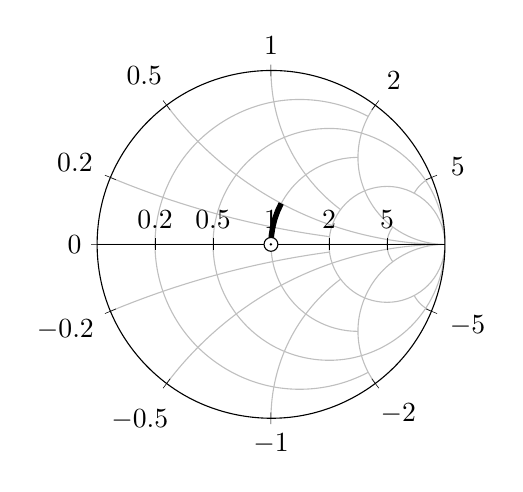
\begin{tikzpicture}
	\begin{smithchart}[
	show origin,
	width=6cm,
	]
	\addplot[mark=none,line width=2]
	coordinates{
		(1, 0) (1, 0.1) (1,0.2) (1,0.3) (1,0.4) (1,0.5) (1,0.5)
	};
	\addplot[mark=none,line width=0.5]
	coordinates{
		(1, 0) (-0.3, 0)  % this one is not drawn outside!!!
	};
	\end{smithchart}
	\end{tikzpicture}
\caption[Smith-Diagramm]{Smith-Diagramm}
\label{fig:smith}
\end{figure}

Ein weiteres Beispiel eines Diagramms ist in Bild~\ref{fig:historamm} dargestellt. Neben der Darstellung eines Histogramms von Messdaten ist eine Gaussfunktion als Näherung angegeben. Eine Erarbeitung eines entsprechenden Diagramms mit EXCEL ist nicht weniger aufwändig und die hier beschriebene Vorgehensweise hat den Vorteil, dass sämtliche Parameter (Achsenbeschriftung, Legende, Farben, Symbole, Beschriftungen) direkt im \LaTeX-Editor vorgenommen werden können.

\begin{figure}[hbt]
	\centering
%	\input{pgfplot/mess5s_histogramm.tex}
	\caption[Histogramm der Häufigkeitsverteilung für eine Zeitmessung]{Histogramm der Häufigkeitsverteilung für die Zeitmessung. Der grau markierte Bereich gibt das Vertrauensintervall für $1 \cdot \sigma $ an.}
	\label{fig:historamm}
\end{figure}

Sollte \textit{pgfplot} trotzdem zu aufwändig erscheinen, so sei das Programm Origin als weitere Empfehlung gegeben. Origin hat einen mächtigen Funktionsumfang, bietet sich gut an, um viele Messdaten zu verwalten und kann auch EXCEL-Dateien einbinden. Das Programm Origin ist als Studentenversion für ca. 100 EUR verfügbar. Die DHBW in Friedrichshafen hat ein paar wenige Netzwerklizenzen. Wenden Sie sich gerne an Hr. Prof. Kibler, sofern Sie Interesse haben.


\begin{figure}[hbt]
	\centering
%	\includegraphics[width=0.7\linewidth]{origin/mess_fehlerbalken_origin}
	\caption{Diagramm erstellt mit Origin}
	\label{fig:origin}
\end{figure}

Mit vielen anderen Programmen lassen sich Diagramme darstellen, orientieren Sie das Erscheinungsbild Ihres Diagramms an den hier gegebenen Beispielen.

%\includegraphics[width=1.4in,height=1.5in,clip,keepaspectratio]{1336385206-131-kibler}}]

% needed in second column of first page if using \IEEEpubid
%\IEEEpubidadjcol

\subsection{Erstellen von Grafiken}

Zur Erstellung von Grafiken kann man im einfachsten Fall PowerPoint benutzen. Mit einem rechten Mausklick auf ein grafisches Element lässt sich dieses als emf-Datei exportieren (emf-Dateien speichern Grafiken vektorbasiert ab). Die emf-Datei kann dann z.B. mit XnView leicht in das pdf-Format übersetzt werden. Mit einem Mac können Sie Grafiken aus PowerPoint direkt im pdf-Format exportieren. Problematisch ist, wie oben schon beschrieben, die Auswahl einer geeigneten Schriftart in der PowerPoint-Grafik.

In \LaTeX~können alternativ grafische Elemente direkt in der Kommandozeile angegeben werden. Hierfür gibt es diverse Packages, z.B. \textit{tikzpicture}. Die Einbindung einer solchen Grafik ist analog zur Vorgehensweise bei einem \textit{pgfplot}-Diagramm. Zur Erstellung einer  \textit{tikzpicture}-Grafik kann das Hilfsprogramm TikzEdt verwendet werden.

\begin{figure}[hbt]
	\centering
	%\includegraphics[width=0.3\linewidth]{bilder/le_block_p}
%	\input{tikz/le_block_tt.tex}
	\caption[Tikzpicture Grafik]{Tikzpicture-Grafik, erstellt mit TikZ.}
	% Die Angabe in der eckigen Klammer würde für den Eintrag in einem Abbildungsverzeichnis verwendet werden. Manche Angaben in der Bildunterschrift sind im verzeichnis ggf. nicht erforderlich.
	\label{fig:le_block_p}
\end{figure}

\subsection{Einsatz von Programmlistings}
Für die Vorlage wird das paket \textit{listings} verwendet. Für die geeignete Markierung von Befehlen kann die verwendete Programmiersprache angegeben werden.



Das Paket \textit{listings} bietet zahlreiche Konfigurationsmöglichkeiten, um die Quellcodedarstellung an die eigenen Wünsche anzupassen. In einer fertig konfigurierten TexLive-Umgebung erfahren Sie mit dem Kommando

\begin{verbatim}
user@client:~> texdoc listings
\end{verbatim}				% Verbatim ist eine einfache Alternative zu lstlistings und erlaubt auf einfache Weise die abgesetzte Darstellung von Code.

mehr über die Möglichkeiten des Pakets.


\subsection{Formeln}
\label{sec:formeln}

Formeln lassen sich in \LaTeX~ganz einfach schreiben, wie bereits zu Beginn der Arbeit auf Seite~\pageref{cha:Einleitung} erwähnt wurde. Es gibt unterschiedliche Umgebungen zum Schreiben von Formeln. Z.B. direkt im Text $v=s/t$ oder abgesetzt

\[F=m \cdot a\]

oder auch, wie in wissenschaftlichen Dokumenten üblich, nummeriert

\begin{equation}
P=\frac{U^2}{R} \quad .
\label{eqn:leistung}
\end{equation}

Mit einem Label in Formel~\ref{eqn:leistung} lassen sich natürlich auch Formeln im Text referenzieren. \LaTeX~verwendet im Formelmodus einen eigenen Schriftsatz, welcher entsprechend der gängigen Konventionen kursive Zeichen verwendet. Sollen im Formelmodus Einheiten in normaler Schriftart eingefügt werden, dann kann dies über den Befehl \textit{\textbackslash mathrm}\{\} erwirkt werden, wie im Quellcode von Formel~\ref{eqn:leistungMitEinh} zu sehen ist.

\begin{equation}
P=\frac{U^2}{R} = \frac{\left( 100~\mathrm{V}\right)^2}{100~\Omega} = 100~\mathrm{W}\quad .
\label{eqn:leistungMitEinh}
\end{equation}

Zum direkten Vergleich sind die Einheiten in Formel~\ref{eqn:leistungMitEinhfalsch} falsch dargestellt:

\begin{equation}
P=\frac{U^2}{R} = \frac{\left( 100~V\right)^2}{100~\Omega} = 100~W
\label{eqn:leistungMitEinhfalsch}
\end{equation}

Das sind nur ein paar wenige Beispiele und es gibt sehr viele Packages, um Besonderheiten in Formeln realisieren zu können. Nennen Sie Formeln nur, wenn diese zum besseren Verständnis auch wirklich nützlich sind.

Nachfolgend sind ein paar beliebig gewählte Beispiele zu mathematischen Ausdrücken aufgeführt:

\subsubsection{Arrays}

Arrays of mathematics are typeset using one of the matrix environments as 
in
\[
\begin{bmatrix}
1 & x & 0 \\
0 & 1 & -1
\end{bmatrix}\begin{bmatrix}
1  \\
y  \\
1
\end{bmatrix}
=\begin{bmatrix}
1+xy  \\
y-1
\end{bmatrix}.
\]
Case statements use cases:
\[
|x|=\begin{cases}
x, & \text{if }x\geq 0\,,  \\
-x, & \text{if }x< 0\,.
\end{cases}
\]
Many arrays have lots of dots all over the place as in
\[
\begin{matrix}
-2 & 1 & 0 & 0 & \cdots & 0  \\
1 & -2 & 1 & 0 & \cdots & 0  \\
0 & 1 & -2 & 1 & \cdots & 0  \\
0 & 0 & 1 & -2 & \ddots & \vdots \\
\vdots & \vdots & \vdots & \ddots & \ddots & 1  \\
0 & 0 & 0 & \cdots & 1 & -2
\end{matrix}
\]

\subsubsection{Delimiters}

See how the delimiters are of reasonable size in these examples
\[
\left(a+b\right)\left[1-\frac{b}{a+b}\right]=a\,,
\]
\[
\sqrt{|xy|}\leq\left|\frac{x+y}{2}\right|,
\]
even when there is no matching delimiter
\[
\int_a^bu\frac{d^2v}{dx^2}\,dx
=\left.u\frac{dv}{dx}\right|_a^b
-\int_a^b\frac{du}{dx}\frac{dv}{dx}\,dx.
\]






\subsubsection{Spacing}

Differentials often need a bit of help with their spacing as in
\[
\iint xy^2\,dx\,dy 
=\frac{1}{6}x^2y^3,
\]
whereas vector problems often lead to statements such as
\[
u=\frac{-y}{x^2+y^2}\,,\quad
v=\frac{x}{x^2+y^2}\,,\quad\text{and}\quad
w=0\,.
\]
Occasionally one gets horrible line breaks when using a list in mathematics such as listing the first twelve primes  \(2,3,5,7,11,13,17,19,23,29,31,37\)\,.
In such cases, perhaps include \verb|\mathcode`\,="213B| inside the inline maths environment so that the list breaks: \(\mathcode`\,="213B 2,3,5,7,11,13,17,19,23,29,31,37\)\,.
Be discerning about when to do this as the spacing is different.




\subsubsection{Equation arrays}

In the flow of a fluid film we may report
\begin{eqnarray}
u_\alpha & = & \epsilon^2 \kappa_{xxx} 
\left( y-\frac{1}{2}y^2 \right),
\label{equ}  \\
v & = & \epsilon^3 \kappa_{xxx} y\,,
\label{eqv}  \\
p & = & \epsilon \kappa_{xx}\,.
\label{eqp}
\end{eqnarray}
Alternatively, the curl of a vector field $(u,v,w)$ may be written 
with only one equation number:
\begin{eqnarray}
\omega_1 & = &
\frac{\partial w}{\partial y}-\frac{\partial v}{\partial z}\,,
\nonumber  \\
\omega_2 & = & 
\frac{\partial u}{\partial z}-\frac{\partial w}{\partial x}\,,
\label{eqcurl}  \\
\omega_3 & = & 
\frac{\partial v}{\partial x}-\frac{\partial u}{\partial y}\,.
\nonumber
\end{eqnarray}
Whereas a derivation may look like
\begin{eqnarray*}
	(p\wedge q)\vee(p\wedge\neg q) & = & p\wedge(q\vee\neg q)
	\quad\text{by distributive law}  \\
	& = & p\wedge T \quad\text{by excluded middle}  \\
	& = & p \quad\text{by identity}
\end{eqnarray*}

\subsubsection{Functions}

Observe that trigonometric and other elementary functions are typeset 
properly, even to the extent of providing a thin space if followed by 
a single letter argument:
\[
\exp(i\theta)=\cos\theta +i\sin\theta\,,\quad
\sinh(\log x)=\frac{1}{2}\left( x-\frac{1}{x} \right).
\]
With sub- and super-scripts placed properly on more complicated 
functions,
\[
\lim_{q\to\infty}\|f(x)\|_q 
=\max_{x}|f(x)|,
\]
and large operators, such as integrals and
\begin{eqnarray*}
	e^x & = & \sum_{n=0}^\infty \frac{x^n}{n!}
	\quad\text{where }n!=\prod_{i=1}^n i\,,  \\
	\overline{U_\alpha} & = & \bigcap_\alpha U_\alpha\,.
\end{eqnarray*}
In inline mathematics the scripts are correctly placed to the side in 
order to conserve vertical space, as in
\(
1/(1-x)=\sum_{n=0}^\infty x^n.
\)






\subsubsection{Accents}

Mathematical accents are performed by a short command with one 
argument, such as
\[
\tilde f(\omega)=\frac{1}{2\pi}
\int_{-\infty}^\infty f(x)e^{-i\omega x}\,dx\,,
\]
or
\[
\dot{\vec \omega}=\vec r\times\vec I\,.
\]





\subsubsection{Command definition}

\newcommand{\Ai}{\operatorname{Ai}} 
The Airy function, $\Ai(x)$, may be incorrectly defined as this 
integral
\[
\Ai(x)=\int\exp(s^3+isx)\,ds\,.
\]

\newcommand{\D}[2]{\frac{\partial #2}{\partial #1}}
\newcommand{\DD}[2]{\frac{\partial^2 #2}{\partial #1^2}}
\renewcommand{\vec}[1]{\text{\boldmath$#1$}}

This vector identity serves nicely to illustrate two of the new 
commands:
\[
\vec\nabla\times\vec q
=\vec i\left(\D yw-\D zv\right)
+\vec j\left(\D zu-\D xw\right)
+\vec k\left(\D xv-\D yu\right).
\]




\subsubsection{Theorems et al.}

\newtheorem{theorem}{Theorem}
\newtheorem{corollary}[theorem]{Corollary}
\newtheorem{lemma}[theorem]{Lemma}
\newtheorem{definition}[theorem]{Definition}

\begin{definition}[right-angled triangles] \label{def:tri}
	A \emph{right-angled triangle} is a triangle whose sides of length~\(a\), \(b\) and~\(c\), in some permutation of order, satisfies \(a^2+b^2=c^2\).
\end{definition}

\begin{lemma} 
	The triangle with sides of length~\(3\), \(4\) and~\(5\) is right-angled.
\end{lemma}

This lemma follows from the Definition~\ref{def:tri} as \(3^2+4^2=9+16=25=5^2\).

\begin{theorem}[Pythagorean triplets] \label{thm:py}
	Triangles with sides of length \(a=p^2-q^2\), \(b=2pq\) and \(c=p^2+q^2\) are right-angled triangles.
\end{theorem}

Prove this Theorem~\ref{thm:py} by the algebra \(a^2+b^2 =(p^2-q^2)^2+(2pq)^2
=p^4-2p^2q^2+q^4+4p^2q^2
=p^4+2p^2q^2+q^4
=(p^2+q^2)^2 =c^2\).





\chapter{Einleitung}
\label{cha:Einleitung}

\section{Problemstellung}
Aus ökonomischer und ökologischer Perspektive ist die Mercedes-Benz AG fortwährend bestrebt die Energieeffizienz in der Automobilproduktion  zu minimieren. Als Kernelement der nachhaltigen Geschäftsstrategie definiert die Ambition 2039 den Weg zur $\text{CO}_2$ neutralen Mobilität unter Berücksichtigung aller \glqq Wertschöpfungsstufen des Automobils – von der Lieferkette über die Produktion bis hin zur Nutzungsphase und Entsorgung der Fahrzeuge\grqq \cite[S.~15]{Stapmanns.2022}. Industrieroboter  (IR) sind ein wesentlicher Bestandteil der Automobilproduktion und damit wichtiger Stellhebel auf dem Weg zur $\text{CO}_2$ neutralen Fertigung und Montage \cite{Maschinenbau.2023}.  Eine $\text{CO}_2$-Reduktion folgt insbesondere aus der Einsparung des Roboter Energieverbrauchs. Damit reiht sich eine Untersuchung zum  Roboter Energieverbrauch in die operative Umweltzielsetzung für die Planung und Produktion der Mercedes-Benz Werke ein \cite[S.~21]{Stapmanns.2022}. Neben dem Energieverbrauch einer Produktion ist an erster Stelle die Ausbringungsmenge und damit die Taktzeit von Relevanz. Infolgedessen lautet die Forschungsfrage der Arbeit, ob ein für die Produktion entwickeltes Roboterprogramm, Software basiert durch das Hinzufügen und Verschieben von Via-Punkten ohne eine signifikante Erhöhung der Bewegungsdauer energetisch optimiert werden? 
%Es wird unterstellt dass eine Anschaffung von Hardware zur Energieeinsparung der Roboter höhere Kosten verursacht als die Umsetzung von Software-Ansätzen. 
% 
\section{Literaturüberblick}
In der vorliegenden Bachelorarbeit wird auf die Themen mechanische Modellierung, Bahnplanung und numerische Optimierung zur Verbesserung der IR Energieeffizienz Bezug genommen. Im Folgenden wird eine Zusammenstellung der verwendeten Literatur aufgeführt. Die Übersicht erhebt keinen Anspruch auf Vollständigkeit,sondern soll vielmehr einen Einstieg in die Thematik bieten. \cite{Carabin.2017} gibt einen Überblick über bestehende Methoden zur Verbesserung der Energieeffizienz von Industrierobotern durch Anpassung der Hard- und/oder Software. Hardwareanpassungen werden in dieser Arbeit nicht untersucht. Aus Gründen der Vollständigkeit werden sie an dieser Stelle zusammenfassend dargestellt. Ein erster Ansatz basiert auf konstruktiven Änderungen an Bauteilen, z. B. dem Austausch schwerer Robotergreifer durch Leichtbaukomponenten. Durch die Reduzierung von Gewicht und Massenträgheit wird das aufzuwendende Drehmoment in den Antrieben des Roboters minimiert. Ein zweiter Ansatz ist die Installation von Systemen oder Komponenten zur Energierückgewinnung im Antriebsstrang während der Bremsphase. \cite{Pellicciari.2015} erarbeitet ein Konzept für den Austausch der zurückgewonnenen Energie über ein Gleichstromnetz (DC-Netz). Dabei wird unter anderem die DC-Netzanbindung des Roboters über eine speziell entwickelte Umrichter-Schnittstelle für den bidirektionalen Energiefluss skizziert.
Einen entscheidenden Beitrag zur Untersuchung softwaregestützter Ansätze zur Energieverbrauchsminimierung leistet \cite{Eggers.2019}.
Softwareseitig werden eine Prozess Optimierung für die Ablaufplanung interagierender IR und die Optimierung der Bahngeometrie für isoliert betrachtete Anlagen unterschieden. Der Energiebedarf Taktzeit unkritischer Anlagen kann durch eine Modifizierung der Verfahrzeit minimiert werden. Im Kontext einer Fließfertigung stellt dies einen vielversprechenden Ansatz dar. In Phasen, in denen die Anlage auf einen vor- oder nachgelagerten Prozess wartet, kann eine Optimierung des Program Override (OR) für den optimalen Energieverbrauch angewandt werden. Der Pfad des Roboters wird dabei nicht verändert. Sodass das Risiko einer Kollision nicht erhöht wird. Eine Ausnahme bilden hierbei miteinander interagierende Roboter, deren Bewegungsabläufe aufeinander abgestimmt werden müssen. Der Ausarbeitung \cite{Eggers.2019} ist hinzuzufügen, dass eine Änderung der Geschwindigkeitsprofile je nach Bewegungsart Auswirkung auf die Bahnplanung und damit den Pfad des Roboters nehmen kann. 
%
% Modell
%
Grundlage für die Optimierung des Energiebedarfs ist die Definition eines geeigneten Modells für den IR. 
Hervorzuheben ist das in \cite{Eggers.2019} beschriebene, erstmalig in \cite{Ziaukas.2017} publizierte und als Patent  \cite{Patent.2016} angemeldete Energiemodell. Im Gegensatz zu den Robotermodell-Beschreibungen in \cite{Pellicciari.2011}, \cite{Sergaki.2002} und \cite{Paryanto.2015} werden nicht nur die Verluste der elektrischen Komponenten detailliert betrachtet, sondern zusätzlich die Betriebszustände des IR unterschieden. 
Entsprechend der Phasen MOTION (Roboter in Bewegung), HOLD (Roboter im Stillstand, Antriebe sind in Regelung) und IDLE (Haltebremsen sind aktiv) wird einer präzise Analyse des Energiebedarf ermöglicht\cite{Ziaukas.2017}. 
%
Ausgangspunkt der numerischen Optimierung ist die Formulierung eines Optimierungsproblems inkl. Definition einer Zielfunktion.  
\cite{Ziaukas.2017} formuliert eine  Reduktion des Energieverbrauch durch Anpassung der Bewegungsdauer und 
%
Ein zweiter Ansatz, der in \cite{Eggers.2019} untersucht wird, ist die Optimierung der Bahngeometrie.  Im Gegensatz zu früheren Ausarbeitungen wird der Ansatz hierbei in umfangreichen praktischen Szenarien validiert. 
Entscheidend für die Durchführung der Optimierung ist die Wahl eines geeigneten Algorithmus.%Im Rahmen einer Ausarbeitung zur Optimierung von Industrierobotern für Hochgeschwindigkeitsanwendungen demonstriert \cite{Gattringer.2013} die praktische Umsetzung der in \cite{Siciliano.2011} beschriebenen System Identifikation.
%
%Optimierer
%
Auf der Grundlage des Modells wird die Bahngeometrie in \Cite{Hansen.2012} mit einem Quasi-Newton-Verfahren, siehe \cite[S.~49]{Papageorgiou.2015} minimiert. \cite{Ziaukas.2017} nutzt für das selbe Ziel einen Active-Set Algorithmus \cite[S.~445]{Luenberger.2021}. Bezüglich der theoretischen Grundlagen der Nichtlinearen-Optimierung wird auf \cite{Nocedal.2006} verwiesen. \cite[S.10~ff.]{Carabin.2017} gibt eine Übersicht weiterer, für den Anwendungsfall bereits angewandter Algorithmen.\cite{Ziaukas.2017} formuliert eine Reduktion des Energieverbrauch neben der Bewegungsdauer durch Minimierung der auftretenden Motordrehmomente. Alternativ wird in \cite{Hansen.2012} die, vom Roboter aufgenommene DC-Netzleistung als Zielfunktion herangezogen.\cite{Lin.2018} schlägt eine Mehrzieloptimierung über den  Energieverbrauch und die Verfahrdauer vor. Die häufig in den Grundlagen zitierte Ausarbeitung \cite{Saravanan.2008} betrachtet in der Optimierung simultan die Minimierung der vom Roboter aufgenommenen Leistung, den Ruck  und die Beschleunigung der einzelnen Gelenke. Abschließend sei die Ausarbeitung  \cite{Bjorkenstam.2013} genannt, welche an Stelle der nichtlinearen Optimierung die Theorie der optimalen Steuerung für eine Energieeffiziente und Kollisionsfreie Roboterbewegung zu Grunde legt.
%
%Trajektorie
%
Eine Notwendigkeit für die Optimierung einer Roboter-Bewegungsbahn ist die Definition der Bahnplanung. Hierbei werden drei wesentliche Ansätze unterschieden. In \cite{Hansen.2012} wird die Point-to-Point (PTP) Bewegungsbahn über eine B-Spline Funktion definiert. Entscheidender Nachteil dabei ist die Übertragung der Funktion auf eine industrielle Robotersteuerung aufgrund fehlenden Entwickler Schnittstellen zur Vorgabe von Sollwerten \cite[S.~55~f.]{Eggers.2019}. Eine praktikablere Umsetzung bietet die Definition und Verschiebung von zusätzlichen Via-Punkten \cite[S.~261~ff.]{Spong.2020}. Nach der Identifikation einer energieoptimierten Gelenkwinkel-Definition wird der Via-Punkt auf die Robotersteuerung übertragen. Der vom Hersteller der Robotersteuerungen implementierte Bahnplanungsansatz wird als black-box angenommen. Infolgedessen sind Abweichungen der, von der Robotersteuerung berechneten Bahn gegenüber der optimierten Bewegungsbahn möglich. \cite{Eggers.2019} vermeidet dieses Problem durch die Berechnung der zu optimierenden Bewegungsbahn auf der Originalsteuerung in einem Software-in-the-Loop (SiL) Ansatz. 
%Gleichzeitig werden damit Nebenbedingungen wie eine Drehmoment Begrenzung in der Antrieben berücksichtigt. 
%
\section{Ausgangslage}
Über die Durchführung einer statistischen Versuchsplanung (design of experiments (DOE)) im Vorfeld der vorliegenden Ausarbeitung konnte der Energieverbrauch eines KUKA KR 270 R2700 ultra IR in einer Laborumgebung um circa 10 \% gesenkt werden. Die Gelenkwinkel der Achsen zwei, drei und fünf wurden als Freiheitsgrade des DOE definiert. Der Versuch umfasst fünf hintereinander ausgeführte Bewegungsabläufe, wobei für jeden ein Via-Punkt zwischen dem Start und Zielwinkel der einzelnen Gelenkwinkel-Trajektorien festgelegt wurde. Der Via-Punkt jeder Trajektorie wurde anfänglich im Mittelpunkt zwischen Start und Zielwinkel der einzelnen Bewegungsabläufe definiert. Diese Via-Punkt Gelenkwinkel wurden mit jedem Versuch variiert. Der Gesamtumfang des Versuchsplans umfasst 20 randomisierte Konfigurationen über die drei Freiheitsgrade je Bewegungsablauf. Für jede Konfiguration wurde die Leistungsaufnahme der Antriebe in 20 Wiederholungen aufgezeichnet. Abschließend wurde für jeden Bewegungsablauf der Energieverbrauch der energieeffizientesten Via-Punkt Konfiguration mit dem Energieverbrauch der initialen Bewegungsbahn verglichen. Für die energieeffizientesten Via-Punkt Konfiguration über alle fünf Bewegungsabläufe weißt der Roboter  einen um 10 \% geringeren Energieverbrauch gegenüber der initialen Bewegungsbahnen auf. Die Forschungsfrage des DOE, ob der Roboter Energieverbrauch für ein bestehendes Roboterprogramm durch Hinzufügen und Verschieben von Via-Punkten minimiert werden kann, wurde verifiziert. Kritisch bewertet wird dabei, dass die Ursachen Grundlage der energetisch besseren Via-Punkte aus dem DOE nicht ersichtlich werden. Diese Lücke wird in der vorliegenden Bachelorarbeit geschlossen.
%
\section{Zielsetzung}
Die Zielsetzung der Arbeit definiert die Umsetzung einer Bahnoptimierung für einen Industrieroboter mit serieller Kinematik. Dafür ist ein in der Produktion eingesetztes Roboterprogramm durch das Hinzufügen und Verschieben von sog. Via-Punkten bezüglich
der aufgenommenen Energie des Roboters bei Abfahren des Programms zu optimieren. Prämisse der Arbeit ist die Identifizierung des energieoptimierten Via-Punkts auf der Grundlage eines Modells. Des Weiteren wird aufgrund strenger Taktzeitanforderungen definiert, dass die Bewegungsdauer der optimierten Bewegungsbahn nicht signifikant höher ausfallen darf als die der initialen Bewegungsbahn. Die vorliegende Arbeit verfolgt nicht das Ziel, dieselbe Modellgenauigkeit durch eine Parameteridentifikation zu erzielen wie \cite{Pellicciari.2011} und \cite{Gattringer.2013}. Von einer Nachbildung des Betriebsverhaltens der Antriebe, siehe \cite{Eggers.2019} und \cite{Ziaukas.2017} wird ebenfalls Abstand genommen. Vielmehr liegt der Fokus darauf die Grundlagen der Mechanischen Modellbildung und Optimierung darzulegen, welche in der o. g. Literatur als bekannt vorausgesetzt sind und nicht näher skizziert werden. 	
%\section{Forschungsfrage} 
\section{Geplantes Vorgehen}
% todo Projektstrukturplan	
Zur Umsetzung dieser Anforderung erfolgt im zweiten Kapitel die Beschreibung der Vorwärtskinematik sowie eine Matlab-Implementierung des rekursiven Newton-Euler-Algorithmus, auf dessen Basis die Dynamik des Roboters simuliert wird. Das dritte Kapitel beschreibt die Bahnplanung.  Basierend auf dieser Definition wird im vierten Kapitel das dynamische Modell validiert. Im fünften Kapitel erfolgt eine Beschreibung des Optimierungsproblems und die Implementierung der Via-Punkt basierten Bahnoptimierung. Anschließend werden die Ergebnisse validiert und bewertet. Die Arbeit schließt mit einer Zusammenfassung der Ergebnisse und der Skizzierung des Ausblicks. 
Die Zeitplanung der Bearbeitung ist im Anhang \ref{add:PSP} hinterlegt.
\chapter{Mechanische Modellbildung}
% todo Bild HMI Roboterkoordinaten ablesen
%
Gegenstand der Modellbildung ist die Definition von Bewegungsgleichungen zur Simulationen der Roboterdynamik. Damit soll die aufgenommene Energie des Roboters entlang einer Bewegungsbahnen bestimmt werden, ohne dass das reale System angesteuert werden muss. ~\autocite[S.~247]{Grimble.2009} Zunächst erfolgt eine Beschreibung der Vorwärtskinematik mithilfe der Denavit-Hartenberg (DH) Konvention.
Nach einer Betrachtung der Geschwindigkeits-Kinematik wird die inverse Dynamik des Systems beschrieben. 
Abschließend wird der Wahrheitsgehalt des Modells überprüft. 

\section{Kinematische Kette}
% um Rieber Skript 2 S 4 ergänzen
Als kinematische Kette wird die Zusammensetzung eines Roboterarms aus $n+1$ Gliedern und $n$ Gelenken definiert. Das letzte Glied der kinematischen Kette wird als Endeffektor bezeichnet. Die Glieder werden von der festen Basis (Glied $0$) bis $n$ durchnummeriert. Mit jedem Glied $i-1$ wird das Gelenk $i$ starr verbunden. Des Weiteren wird jedem Glied $i$ ein fest verbundenes Koordinatensystem $o_ix_iy_iz_i$ zugeordnet. Eine Aktuierung des Gelenks $i$ führt zu einer Bewegung von Glied $i$ und Koordinatensystem KS$\left\{i\right\}$. Die Gelenke weisen einen Freiheitsgrad (degree-of-freedom (DOF)) $q_i$ auf und können als Dreh- oder Schubgelenke ausgeführt werden. Die Gelenkvariable $q_i$ entspricht dem Rotationswinkel $\theta_i$ bzw. der Translation $d_i$. 

\section{Vorwärtskinematik}
Über die Vorwärtskinematik erfolgt eine geometrische Beschreibung der Endeffektor Bewegung des Roboters entlang der kinematischen Kette. Entsprechend der Gelenkvariablen wird dabei die Position und Orientierung (Pose) des Endeffektors im Basis-Koordinatensystem berechnet. Ausgehend vom Basis-Koordinatensystem werden homogene Transformationsmatrizen $\bm{A}(i) = \bm{T}^{i-1}_i$ zwischen zwei aufeinanderfolgenden Koordinatensystemen $0_{i-1}x_{i-1}y_{i-1}z_{i-1}$ und $0_ix_iy_iz_i$ der kinematischen Kette definiert. $\bm{T}^{i-1}_i$ (Lie-Gruppe SE(3)) repräsentiert die  Rotation und Translation des KS$\left\{i\right\}$ im $\left\{i-1\right\}$. Die Transformationsmatrizen sind abhängig von der Konfiguration der Gelenkvariablen $q_i$ des Roboters.
\begin{align}
	\bm{A}_i = \bm{A}_i(q_i)
\end{align}
Eine Repräsentation der Endeffektor-Pose $H$ im Basis-Koordinatensystem wird über eine Multiplikation der homogenen Transformationsmatrizen entlang der kinematischen Kette erreicht. 
\begin{align}
	\label{eqn:homogeneTransformation}
	\bm{H} = \bm{T}^0_n = \bm{A}_1(q_1) ... \bm{A}_n(q_n)
\end{align}
\begin{align}
	\bm{H} =\begin{bmatrix} \bm{R}^0_n &\quad \bm{o}^0_n\\ \mathbf{0}_{1x3} &\quad 1\end{bmatrix}
\end{align}
Der Spaltenvektor $\bm{o}^0_n$ repräsentiert die Koordinaten des Ursprungs des Endeffektor-Koordinatensystems im Basis-Koordinatensystem. Die $3 \times 3 $ Matrix $\bm{R}^n_0$ entspricht der Rotation des Endeffektor-Koordinatensystems gegenüber dem Basis-Koordinatensystem. \autocite{Spong.2020} 
%
\section{Denavit-Hartenberg Konvention}
Eine Methode zur Bestimmung der homogenen Transformationsmatrizen ist die, nach  dem Physiker Jacques Denavit und dem Ingenieur Richard Hartenberg benannte Denavit-Hartenberg Konvention. Diese besagt, dass jede homogene Transformation $\bm{A}_i$ als Produkt vier nacheinander ausgeführter elementarer Transformationen ausgedrückt werden kann. 
\begin{align}
	\label{eqn:elementarTransformation}
	A_i &= \text{Rot}_{z,\theta_i}\text{Trans}_{z,d_i}\text{Trans}_{x,a_i}\text{Rot}_{x,\alpha_i} \\
	&= \left[\begin{matrix}
		c_{\theta_i} &\quad -s_{\theta_i} &\quad 0 &\quad 0 \\
		s_{\theta_i} &\quad c_{\theta_i} &\quad 0 &\quad 0 \\
		0 &\quad 0 &\quad 1 &\quad 0 &\quad \\ 
		0 &\quad 0 &\quad 0 &\quad 1 &\quad 
	\end{matrix}\right] 
	\left[\begin{matrix}
		1 &\quad 0 &\quad 0 &\quad 0 \\
		0 &\quad 1 &\quad 0 &\quad 0 \\
		0 &\quad 0 &\quad 1 &\quad d_i &\quad \\ 
		0 &\quad 0 &\quad 0 &\quad 1 &\quad 
	\end{matrix}\right] \notag \\
	& \times
	\left[\begin{matrix}
		1 &\quad 0 &\quad 0 &\quad a_i \\
		0 &\quad c_{\alpha_i} &\quad -s_{\alpha_i} &\quad 0 \\
		0 &\quad s_{\alpha_i} &\quad c_{\alpha_i} &\quad 0 &\quad \\ 
		0 &\quad 0 &\quad 0 &\quad 1 &\quad 
	\end{matrix}\right]
	\left[\begin{matrix}
		1 &\quad 0 &\quad 0 &\quad 0 \\
		0 &\quad 1 &\quad 0 &\quad 0 \\
		0 &\quad 0 &\quad 1 &\quad 0 &\quad \\ 
		0 &\quad 0 &\quad 0 &\quad 1 &\quad 
	\end{matrix}\right]
	\notag \\
	c = cos\notag \\
	s = sin \notag 
\end{align}
Die Parameter entsprechen dem Gelenkwinkel $\theta_i$, dem Gelenkabstand $d_i$, der Armelementlänge $a_i$ und der Verwindung $alpha_i$, wobei $d_i$, $a_i$ und $alpha_i$ konstant sind.

%\subsection{Festlegung der Koordinatensysteme}
Abbildung \ref{fig:kr210} zeigt den zu untersuchenden KUKA KR210 R2700-2 Industrieroboter. Die Bezeichnung der Maschine gibt Auskunft über ihre technischen Daten.  Die Nenn-Traglast beträgt 210 kg. Die maximale Reichweite des Roboters liegt bei 2701 mm. Weitere Informationen sind dem Datenblatt, siehe Anhang \ref{add:datenblatt} zu entnehmen.  
%
\begin{figure}[tbph]
	\centering
	\includegraphics[width=0.8\linewidth]{images/KR210}
	\caption{KUKA KR210 R2700-2}
	\label{fig:kr210}
\end{figure}
%
Im ersten Schritt werden die Achsen $z_i, \ i = 0,...,n-1, n=6$,	siehe Abbildung \ref{fig:zachsen} definiert. 
%
\begin{figure}[tbph]
	\centering
	\includegraphics[width=0.5\linewidth]{images/zAchsen}
	\caption[]{Festlegung der z-Achsen}
	\label{fig:zachsen}
\end{figure}
%
Im zweiten Schritt wird das Basiskoordinatensystem ${0}$ definiert, wobei der Ursprung $\bm{o}_0$ auf der Achse $z_0$ platziert wird. Die Festlegung entspricht dem ROBROOT Koordinatensystem, welches der Robotersteuerung bekannt ist. Diese Festlegung erlaubt eine Überprüfung der Vorwärtskinematik mithilfe der, von der KRC (KUKA Robot Control) berechneten kartesischen Koordinaten. Des Weiteren werden, siehe Abbildung \ref{fig:KS} aufsteigend die Koordinatensysteme KS$\{i\},i=1,...,n-1$ basierend auf KS$\left\{i-1\right\}$, sowie das rot hervorgehobene Endeffektor-Koordinatensystem $0_6x_6y_6z_6$ platziert. Es werden folgende Regeln berücksichtigt.  
%
\begin{figure}[tbph]
	\centering
	\includegraphics[width=0.5\linewidth]{images/KS}
	\caption{Festlegung der Koordinatensysteme}
	\label{fig:KS}
\end{figure}
%
\begin{itemize}
	\item Falls sich $z_i$ und $z_{i-1}$ scheiden, ist der Ursprung $\bm{o}_i$ in den Schnittpunkt zu legen. Die Achse $x_i$ wird rechtwinklig zur $z_{i-1}-z_i$-Ebene definiert. (gilt für KS$\left\{4\right\}$ und KS$\left\{5\right\}$)
	\item Falls  $z_i$ und $z_{i-1}$ parallel sind, wird der Ursprung $\bm{o}_i$ auf die Achse $z_i$ gelegt. Die Achse $x_i$ wird parallel zur gemeinsamen Normale von $z_i$ und $z_{i-1}$	im Punkt $\bm{o}_i$ definiert. (gilt für KS$\left\{2\right\}$)
	\item Falls  $z_i$ und $z_{i-1}$ nicht koplanar sind, wird der Ursprung $\bm{o}_i$ auf den Schnittpunkt der Achse $z_i$ mit der gemeinsamen Normalen von $z_i$ und $z_{i-1}$  gelegt. Die Achse $x_i$ ist die gemeinsamen Normale von $z_i$ und $z_{i-1}$. (gilt für KS$\left\{1\right\}$ und KS$\left\{3\right\}$)
	\item die Achse $y_i$ vervollständigt das rechtshändige, kartesische Koordinatensystem
\end{itemize} 
%
Im nächsten Schritt werden DH-Parameter, identifiziert.  $\theta_i$ entspricht der Rotation um $z_{i-1}$, sodass $x_{i-1}||x_i$. Der Parameter $d_i$ drückt die Translation entlang $z_{i_1}$ bis zum Schnittpunkt S von $z_{i-1}$ und $x_i$ aus. Der Parameter $a_i$ entspricht der Translation entlang $x_i$, um den Schnittpunkt S in den Ursprung $o_i$ zu überführen. $\alpha_i$ ist die Rotation um $x_i$, sodass $z_{i-1}$ in $z_i$ überführt wird. Aus den Elementartransformationen, siehe Gleichung \ref{eqn:elementarTransformation} wird die Gesamttransformationen entsprechend der Gleichung \ref{eqn:homogeneTransformation} berechnet. Tabelle \ref{tab:dh} listet die identifizierten DH-Parameter. 
%
\begin{table}[tbph]
	\centering
	\begin{tabular}{|c|c|c|c|c|}
		\hline
		Gelenk & theta & d [m] & a [m] & alpha \\
		\hline
		1& 0 & 0,645 & 0,330 & $-90^\circ$ \\
		\hline
		2& $-90^\circ$ & 0 & 1,150 & 0 \\
		\hline
		3& 0 & 0 & 0,115 & $90^\circ$ \\
		\hline
		4& 0 & -1,220 & 0 & $-90^\circ$ \\
		\hline
		5& 0 & 0 & 0 & $-90^\circ$ \\
		\hline
		6& $90^\circ$ & 0,215 & 0 & 0 \\
		\hline
	\end{tabular}
\caption{Denavit-Hartenberg Parameter}
\label{tab:dh}
\end{table}
%
Eine Verarbeitung der Gelenkwinkel, welche in der KRC für eine bestimmte Pose definiert sind, bedingt eine Anpassung DH-Parameter. Der Lieferant KUKA definiert die Achse $z_{1}$ um 180° rotiert ggü. der o. g. Festlegung. Folglich werden die, in der Robotersteuerung gegebenen Winkel des ersten Gelenks  mit -1 multipliziert, bevor eine Weiterverarbeitung im Modell erfolgt. Des Weiteren werden vom dritten Winkel 90° subtrahiert, bevor der Wert dem Modell übergeben wird. Die Vorwärtskinematik ist über drei verschiedene Posen am realen System verifiziert. Dabei ist festzustellen, dass in der Robotersteuerung die Biegung der Glieder berücksichtigt wird, wohingegen in der oben gezeigten Definition von einem Starrkörper-Modell ausgegangen wird. 
Die Implementierung der DH-Transformation ist im Anhang \ref{add:dh}  aufgeführt. 
%
\section{Geschwindigkeits-Kinematik}
Die Geschwindigkeits-Kinematik definiert die lineare Endeffektor-Geschwindigkeit, sowie die  Endeffektor-Winkelgeschwindigkeit in Abh{\"a}ngigkeit der Gelenkwinkelgeschwindigkeiten des Roboters. Eine mathematische Beschreibung des Zusammenhangs erfolgt {\"u}ber die Jacobi-Matrix der Vorw{\"a}rtskinematik.~\autocite[S.~101]{Spong.2020} Zur Aufstellung der Jacobi-Matrizen werden zunächst grundlegende Definitionen betrachtet. Die Herleitung der Zusammenhänge ist ~\autocite[S.~79--80]{Kemmetmueller.2023} und ~\autocite[S.~106]{Spong.2020} entnommen. Die Rotation eines Starrk{\"o}rpers um eine feste Drehachse wird über die Beziehung $\bm{\omega} = \dot{\theta}\bm{k}$ ausgedr{\"u}ckt. Dabei sind $\dot{\theta}$ die zeitliche Ableitung des Gelenkwinkels $\theta$ und $\bm{k}$ der Einheitsvektor der Drehachse. Die lineare Geschwindigkeit eines Punktes P, welcher um die Drehachse rotiert, ergibt sich zu $\bm{v} = \bm{\omega} \times \bm{r}$. Wobei der Vektor $\bm{r}$ die Position des Punktes P orthogonal auf der Drehachse $\bm{k}$ angibt.~\autocite[S.~102]{Spong.2020} 
%
\subsection{Schiefsymmetrische Matrizen}
Die Berechnung der Geschwindigkeits-Kinematik l{\"a}sst sich durch Verwendung Schiefsymmetrischer Matrizen vereinfachen. Eine $n\times n$ Matrix $\bm{S}$ ist schief symmetrisch, wenn 
\begin{equation}
	\label{eqn:skewsymmetric}
	\bm{S}^T+\bm{S}=0.
\end{equation}
Damit hat jede schiefsymmetrische $3\times3$ Matrix die Form
\begin{align}
	\bm{S} = \left[\begin{matrix}
		0 &\quad -s_3 &\quad s_2  \\
		s_3 &\quad 0 &\quad -s_1  \\
		-s_2 &\quad s_1 &\quad 0  
	\end{matrix}\right].
\end{align}
Für weitere Eigenschaften schiefsymmetrischer Matrizen wird auf die referenzierte Literatur ~\autocite[S.~104]{Spong.2020} verwiesen. Für die Drehmatrix $\bm{R} = \bm{R}(\theta) \in SO(3)$, deren Elemente Funktionen der Drehwinkel $\theta\left(t\right)$ sind, gilt 
\begin{equation}
	\label{eqn:einheitsmatrix}
	\bm{R}(\theta)\bm{R}(\theta)^T = E.
\end{equation}
%
\subsection{Drehwinkelgeschwindigkeit}
Die Ableitung beider Terme der Gleichung \ref{eqn:einheitsmatrix} ergibt
\begin{equation} 
	\frac{\text{d}}{\text{d}\theta}\left[\bm{R}(\theta)\bm{R}(\theta)^T\right] = 	\left[\frac{\text{d}}{\text{d}\theta} {\bm{R}}(\theta)\right]\bm{R}(\theta)^T + \bm{R}(\theta)\left[\frac{\text{d}}{\text{d}\theta} {\bm{R}}(\theta)^T\right] = 0
\end{equation} 
Unter Berücksichtigung der Eigenschaft schiefsymmetrischer Matrizen, siehe Gleichung \ref{eqn:skewsymmetric} folgt
\begin{equation}
	\label{eqn:skewsymm}
	\bm{S} = \left[\frac{\text{d}}{\text{d}\theta}{\bm{R}}(\theta)\right]\bm{R}(\theta)^T  = -\bm{R}(\theta)     \left[\frac{\text{d}}{\text{d}\theta}{\bm{R}}(\theta)^T\right].
\end{equation} 
%
Daraus folgt
%
\begin{equation}
	\frac{\text{d}}{\text{d}\theta}\bm{R}(\theta) = \bm{SR}(\theta)
\end{equation} 
%
Die zeitliche Ableitung der Rotationsmatrix $\bm{R} = \bm{R}(t) \in SO(3)$ lautet
%
\begin{equation}
	\frac{\text{d}}{\text{d}t}\bm{R}(t) = \bm{S}\left(\bm{\omega}(t)\right)\bm{R}(t)
\end{equation} 
%
Für Verkettete Rotationen gilt
%
\begin{equation}
	\frac{\text{d}}{\text{d}t}\bm{R}^0_n(t) = \bm{S}\left(\bm{\omega}^0_{0,n}(t)\right)\bm{R}^0_n(t)
\end{equation} 
\begin{equation}
	\bm{\omega}^0_{0,n} = \bm{\omega}^0_{0,1} + \bm{R}^0_1\bm{\omega}^1_{1,2} + \bm{R}^0_2\bm{\omega}^2_{2,3} + ... + \bm{R}^0_{n-1}\bm{\omega}^{n-1}_{n-1,n}
\end{equation} 
%
%Die Elemente von $\bm{S}$ resultieren aus den Winkelgeschwindigkeiten $\omega = \left[\omega_x~\omega_y~\omega_z\right]^T$.
%\begin{equation}
%	\bm{S} = \left[\begin{array}{ccc}
	%		0&-\omega_z&\omega_y  \\
	%		\omega_z&0&-\omega_x  \\
	%		-\omega_y&\omega_x&0  \\
	%	\end{array} \right]
%\end{equation}
%
\subsection{Lineare Geschwindigkeit}
Für die Lineare Geschwindigkeit eines Punktes werden nachfolgend zwei Szenarien unterschieden. In beiden Fällen ist der Punkt P fest mit dem KS$\left\{i\right\}$ verbunden. Im ersten Fall wird eine Rotation des KS$\left\{i\right\}$ relativ zum KS$\left\{0\right\}$ betrachtet. 
\begin{equation}
	\bm{p}^0 = \bm{R}^0_i(t)\bm{p}^i
\end{equation}
%
\begin{equation}
	\dot{\bm{p}}^0 = \bm{\omega}^0_{0,i}\times\bm{p}^0
\end{equation}
%
Im zweiten Fall bewegt sich KS$\left\{i\right\}$ rotatorisch und translatorisch relativ zu KS$\left\{0\right\}$. 
\begin{equation}
	\bm{p}^0 = \bm{R}^0_i(t)\bm{p}^i + \bm{o^0_i}
\end{equation}
%
\begin{equation}
	\dot{\bm{p}}^0 = \bm{\omega}^0_{0,i}\times\bm{p}^0 + \dot{\bm{o^0_i}}
\end{equation}
Auf eine Beschreibung des Szenarios, dass sich P gegenüber KS$\left\{i\right\}$ bewegt, wird verzichtet.
%
\subsection{Jacobi-Matrizen}
Die lineare Geschwindigkeit $\bm{v}^0_n$ des Endeffektors, sowie seine Winkelgeschwindigkeit $\bm{\omega}^0_{0,i}$ im  KS$\left\{0\right\}$ lassen sich über die $3\times n$-Jacobi-Matrizen $\bm{J}_v$ und $\bm{J}_{\omega}$ berechnen. 
%
\begin{equation}
	\bm{v}^0_n = \bm{J}_v \dot{\bm{q}} = \left[\bm{J}_{v1 \ \bm{J}_{v2}} \ ...\  \bm{J}_{vn}\right] \dot{\bm{q}}
\end{equation}
%
\begin{equation}
	\bm{\omega}^0_{0,i} = \bm{J}_{\omega} \dot{\bm{q}}  = \left[\bm{J}_{\omega1 \ \bm{J}_{\omega2}} \ ...\  \bm{J}_{\omega n}\right] \dot{\bm{q}}
\end{equation}
%
\begin{equation}
	\bm{J}_{vi} = \begin{cases} 
		\bm{z}^0_{i-1} \times (\bm{o}^0_{n} - \bm{o}^0_{i-1}) & \text{falls Gelenk } i \text{ vom Typ } \text{R} \\
		\bm{z}^0_{i-1} & \text{falls Gelenk } i \text{ vom Typ } \text{T}
	\end{cases}
\end{equation}
%
\begin{equation}
	\bm{J}_{\omega i} = \begin{cases} 
		\bm{z}^0_{i-1} = \bm{R}^0_{i-1}\bm{e}_3 & \text{falls Gelenk } i \text{ vom Typ } \text{R} \\
		\mathbf{0}_{3 \times 1} & \text{falls Gelenk } i \text{ vom Typ } \text{T}
	\end{cases}
\end{equation}
%
\begin{itemize}
	\item Ein Gelenk vom Typ R ist ein Rotationsgelenk.
	\item Ein Gelenk vom Typ T ist ein Translationsgelenk.
\end{itemize}
%
Die Notation ist \autocite{Rieber.2022} entnommen.
%
% todo Relevanz Geeschwindigkeitskinematik
%
\section{Dynamik}
Ziel des Kapitels ist die Lösung des inversen dynamischen Problems, der Berechnung der aufzubringenden Momente in den sechs Gelenken des Roboters bei Ansteuerung entlang einer Bewegungsbahn. \autocite[S.~247]{Grimble.2009} 
Die Bewegungsgleichungen werden zunächst formal mithilfe der Euler-Lagrange Gleichungen formuliert. Anschließend folgt die numerisch effiziente Implementierung  über den Rekursiven-Newton-Euler-Algorithmus (RNEA).  \autocite[S.~247]{Grimble.2009} 
%
\subsection{Euler-Lagrange Gleichungen}
Die Lagrange Funktion $L$ eines mechanischen Systems entspricht der Differenz der kinetischen Energie $K$ und potentiellen Energie $P$.~\autocite[S.~175]{Spong.2020}
\begin{equation}
	L = K-P 
\end{equation}
%
%Für einen bewegten Starrkörper mit der Geschwindigkeit $\dot{q}$ und Masse $m$ folgt unter Einwirkung der Fallbeschleunigung $g$ die Formulierung. 
%
%\begin{equation}
%	L = \frac{1}{2}m\dot{q}^2 - mgq
%\end{equation}
%
Die Euler-Lagrange-Gleichung wird über den folgenden Ausdruck beschrieben. Dabei entspricht die Ordnung $n$ des Systems der Anzahl generalisierter Koordinaten \footnote{Voneinander unabhängige Koordinaten, welche den aktuellen Systemzustand vollständig beschreiben \cite{Engelke.2008}}, bzw. im Anwendungsfall den sechs rotatorischen Gelenkkoordinaten ($\theta_1$,...,$\theta_6$). Die Größe $\tau_i$ repräsentiert generalisierte Kräfte \footnote{Kräfte und Momente}. Im Anwendungsfall werden die Antriebsmomente in den Gelenken betrachtet. 
%
\begin{equation}
	\frac{d}{dt} \frac{\partial{L}}{\partial{\dot{\bm{q}_i}}}- \frac{\partial{L}}{\partial{\bm{q}_i}} = \bm{\tau}_i \ ;  \ i = 1,...,n 
\end{equation}
%
\begin{equation}
	\frac{\partial{L}}{\partial{\dot{q}}} = \frac{\partial{K}}{\partial{\dot{q}}}
\end{equation}
%
\begin{equation}
	\frac{\partial{L}}{\partial{\bm{q}}} = -\frac{\partial{P}}{\partial{\bm{q}}}
\end{equation}
%
Die kinetischen Energie des Roboters entspricht der Gleichung  \ref{eqn:ekin}
\begin{equation}
	\label{eqn:ekin}
	K = \frac{1}{2} \dot{\bm{\bm{q}}}^T \left[\sum_{i=1}^{n} \left( m_i \bm{J}_{v_i}(\bm{q})^T \bm{J}_{v_i}(\bm{q}) + \bm{J}_{\omega_i}(\bm{q})^T \bm{R}^0_i(\bm{q}) \bm{I}^{i}_{i} \bm{R}^0_i(\bm{q})^T \bm{J}_{\omega_i}(\bm{q}) \right) \right]\dot{\bm{\bm{q}}}
\end{equation}
%
Der Ausdruck in der Klammer wird als Massenmatrix $\bm{M}(\bm{q})$ bezeichnet. 
Die Massen $m_i$ sind einem Computer Aided Design- (CAD) Modell, welches vom Hersteller bereitgestellt wird, entnommen. 
Die Trägheitstensoren $\bm{I}^{i}_{i}$, bezogen auf den Masseschwerpunkt des Verbindungsglieds $i$ sind relativ zu den Gelenkkoordinatensystemen orientiert und damit für alle Konfigurationen des Roboters konstant. 
Über das CAD-Modell werden die Trägheitstensoren $\bm{I}^{0}_{i}$, bezogen auf den Masseschwerpunkt relativ zum ROBROOT-KS (KS$\left\{0\right\}$) bereitgestellt. Die gewünschte Umrechnung erfolgt mithilfe der Ähnlichkeitstransformation 
%
\begin{equation}
	\label{eqn:similarity}
	\bm{I}^{i}_{i} = {\bm{R}^{0}_i}^T \bm{I}^{0}_{i} \bm{R}^0_i.
\end{equation}
%
Die potentielle Energie wird über den Ausdruck \ref{eqn:epot} berechnet.
%
\begin{equation}
	\label{eqn:epot}
	P = \sum_{i=1}^{n} m_i \bm{g}^T\bm{r^0_{C_i}}
\end{equation}
%
Der Vektor $g = [0,0,-9.81]^T~\frac{\text{m}}{\text{s}}$ entspricht der Fallbeschleunigung, ausgedrückt im KS$\left\{0\right\}$. Der Vektor $r^0_{C_i}$ definiert die Lage des Masseschwerpunkts von Körper $i$ im  KS$\left\{0\right\}$. Für die Herleitung der Bewegungsgleichungen \ref{eqn:bewegungsgleichungen} wird auf die Literatur \autocite[S.~180 ff.]{Spong.2020} verwiesen. Hierbei wird ersichtlich, dass die numerische Bestimmung von $\tau$ über die partiellen Ableitungen von $K$ und $P$ insbesondere in den letzten Gliedern der kinematischen Kette einen hohen Berechnungsaufwand erfordert, weshalb das Modell über den RNEA implementiert ist. 
%
\begin{equation}
	\label{eqn:bewegungsgleichungen}
	\bm{M}(\bm{q})\ddot{\bm{q}} + \bm{C}(\bm{q},\dot{\bm{q}})\dot{\bm{q}} + \bm{g}(\bm{q}) = \bm{\tau}
\end{equation}
%
Der Term $\bm{C}(\bm{q},\dot{\bm{q}})\dot{\bm{q}}$ berücksichtigt die Einflüsse der Corioliskraft und Zentrifugalkraft\footnote{Für die Scheinkräfte in rotierenden Bezugssystemen wird auf die Literatur ~\autocite[S.~159]{Roth.2016} verwiesen}. Der Vektor $\bm{g}(\bm{q})$ berücksichtigt die Gravitation.
%
\subsection{Rekursiver-Newton-Euler-Algorithmus}
%
Der Ansatz sieht vor, jedes Verbindungsglied der kinematischen Kette und die, auf dieses wirkenden Kräfte $ -\boldsymbol{f}_{i+1} $ und $ \boldsymbol{f}_i $ im Einzelfall zu betrachten. Ziel ist die Berechnung, der im zugehörigen Gelenk wirkenden Drehmomente $\bm{\tau}$. Zur Berechnung der Drehmomente $\bm{\tau}$ in den Gelenken wird der Vektor $\bm{\mu}$ eingeführt. $\bm{\mu}_i$ hat die Dimension $3 \times n$ und repräsentiert das Drehmoment im Gelenk $i$ des Verbindungsglieds $i$. $\bm{\tau}_i$ entspricht dem Betrag Drehmoments je Gelenk $i$. Abbildung \ref{fig:rnea} zeigt die, zu berücksichtigenden Größen am Beispiel eines generischen Verbindungsglieds $i$.
%
\begin{figure}[tbph]
	\centering
	\includegraphics[width=1\linewidth]{images/rnea}
	\caption{generisches Verbindungsglied \cite[S.~283]{Siciliano.2011}}
	\label{fig:rnea}
\end{figure} 
%
\subsubsection*{Kräfte und Momente}
\setlist{noitemsep}
\begin{itemize}
	\item $ \boldsymbol{f}_i $ - Kraft, die vom Verbindungsglied $ i-1 $ auf das Verbindungsglied $ i $ ausgeübt wird
	\item $ -\boldsymbol{f}_{i+1} $ - Kraft, die vom Verbindungsglied $ i+1 $ auf das Verbindungsglied $ i $ ausgeübt wird
	\item $ \boldsymbol{\mu}_i $ - Drehmoment, welches vom Verbindungsglied $ i-1 $ auf das Verbindungsglied $ i $ im KS$\left\{i-1\right\}$ des dazugehörigen Gelenks $i$ ausgeübt wird
	\item $ -\boldsymbol{\mu}_{i+1} $ - Drehmoment, welches vom Verbindungsglied $ i+1 $ auf das Verbindungsglied $ i $ im KS$\left\{i\right\}$ des dazugehörigen Gelenks $i+1$ ausgeübt wird
\end{itemize}
%
Die Implementierung des RNEA sieht vor, alle Größen bezogen auf das KS$\left\{i\right\}$ des fest damit verbundenen Verbindungsglieds $i$ zu beziehen. Daraus resultieren die Kräfte und Momente mit der Notation $ \boldsymbol{f}_{i}^{i} $ und $ \boldsymbol{\mu}_i^{i} $. Nachfolgend werden die Parameter der Verbindungsglieder eingeführt. Alle Vektoren beziehen sich ebenfalls auf das KS$\left\{i\right\}$, sodass die Parameter als Konstante weiterverarbeitet werden können. Die Werte der Systemparameter sind im Anhang \ref{add:systemparameter} aufgeführt.
%
\subsubsection*{Parameter}
\setlist{noitemsep}
\begin{itemize}
	\item $ m_i $ - Masse des Verbindungsglieds $i$
	\item $ \bm{I}^{i}_{i} $ - Trägheitstensor des Verbindungsglieds $i$ im fest damit verbundenen KS$\left\{i\right\}$ 
	\item $ \boldsymbol{r}^{i}_{i-1,C_i} $ - Vektor vom Ursprung des KS$\left\{i-1\right\}$ zum Masseschwerpunkt $ C_i $ des Verbindungsglieds $i$ im KS$\left\{i\right\}$ 
	\item $ \boldsymbol{r}^{i}_{i,C_i} $ - Vektor vom Ursprung des KS$\left\{i\right\}$ zum Masseschwerpunkt $ C_i $ im KS$\left\{i\right\}$ 
	\item $ \boldsymbol{r}^{i}_{i-1,i} $ - Vektor vom Ursprung des KS$\left\{i-1\right\}$ zum Ursprung des  KS$\left\{i\right\}$ im KS$\left\{i\right\}$ 
	\item $ i_i$ - Übersetzungsverhältnis der Getriebe
\end{itemize}
%
\subsubsection*{Geschwindigkeiten und Beschleunigungen}
\setlist{noitemsep}
\begin{itemize}
	\item $ \dot{\boldsymbol{p}}_{C_i} $ - Lineare Geschwindigkeit im Masseschwerpunkt $ C_i $ 
	\item $ \dot{\boldsymbol{p}}_i $ - Lineare Geschwindigkeit im Ursprung des KS$\left\{i\right\}$
	\item $ \boldsymbol{\omega}_i $ - Winkelgeschwindigkeit des Verbindungsglieds $i$
	\item $ \ddot{\boldsymbol{p}}_{C_i} $ - Lineare Beschleunigung im Masseschwerpunkt $ C_i $
	\item $ \ddot{\boldsymbol{p}}_i $ - Lineare Beschleunigung im Ursprung des KS$\left\{i\right\}$
	\item $ \boldsymbol{\dot{\omega}}_i $ - Winkelbeschleunigung des Verbindungsglieds $i$
\end{itemize}
%
Mit Kenntnis der Größen $\bm{q}, \dot{\bm{q}}, \ddot{\bm{q}}$ aus der Bahnplanung des Roboters und unter Festlegung der Startbedingungen $\bm{\omega}_0 = 0,~ \ddot{\bm{p}_0}-g = [0,0,-9.81]^T,~ \ddot{\bm{\omega}_0} = 0$  erfolgt sukzessive die Berechnung der Geschwindigkeiten und Beschleunigungen für jedes Verbindungsglied des Roboters vom ersten bis zum sechsten. Ein Endeffektor ist am Versuchsroboter nicht verbaut. Die der Literatur ~\autocite[S.~287~f.]{Grimble.2009} entnommenen Gleichungen \ref{eqn:rnea0}, \ref{eqn:rnea1}, \ref{eqn:rnea2} und  \ref{eqn:rnea3} werden nachfolgend aufgezeigt. Diese gelten ausschließlich für rotatorische Gelenke, da der betrachtete KUKA KR210 R2700-2 eine RRR-Kinematik mit Zentralhand (rotatorische Funktionen Drehen, Nicken, Gieren) aufweist. 
%
\begin{equation}
	\label{eqn:rnea0}
	\bm{\omega}^i_i = {\bm{R}^{i-1}_i}^T  \left( \bm{\omega}^{i-1}_{i-1} +\dot{\theta}_i\bm{z_0} \right)
\end{equation}
%
\begin{equation}
	\label{eqn:rnea1}
	\dot{\bm{\omega}}^i_i = {\bm{R}^{i-1}_i}^T  \left( \dot{\bm{\omega}}^{i-1}_{i-1} +\ddot{\theta}_i\bm{z_0} +\dot{{\theta}}_i\bm{\omega}^{i-1}_{i-1} \times \bm{z}_0 \right)
\end{equation}
%
\begin{equation}
	\label{eqn:rnea2}
	\ddot{\bm{p}}^i_i = {\bm{R}^{i-1}_i}^T  \ddot{\bm{p}}^{i-1}_{i-1} + \dot{\bm{\omega}}^{i}_{i} \times \bm{r}^{i}_{i-1,i} + {\bm{\omega}}^{i}_{i} \times \left(  {\bm{\omega}}^{i}_{i} \times \bm{r}^{i}_{i-1,i} \right)
\end{equation}
%
\begin{equation}
	\label{eqn:rnea3}
	\ddot{\bm{p}}^i_{C_i} = \ddot{\bm{p}}^{i}_{i} + \dot{\bm{\omega}}^{i}_{i} \times \bm{r}^{i}_{i,C_i} + {\bm{\omega}}^{i}_{i} \times \left(  {\bm{\omega}}^{i}_{i} \times \bm{r}^{i}_{i,C_i} \right)
\end{equation}
%
Im nächsten Schritt erfolgt die rekursive Berechnung der Kräfte und Drehmomente. Der Algorithmus startet beginnt mit der Berechnung für das sechste Gelenk, gemäß der Gleichungen \ref{eqn:rnea4}, \ref{eqn:rnea5} und \ref{eqn:rnea6} und endet für das erste Gelenk. $\bm{f}^{n+1}_{n+1}$ und $\bm{\mu}^{n+1}_{n+1}$ werden zu 0 angenommen. 
%
\begin{equation}
	\label{eqn:rnea4}
	\bm{f}^{i}_{i} = \bm{R}^{i}_{i+1} \bm{f}^{i+1}_{i+1} + m_i\ddot{\bm{p}}^{i}_{C_i}
\end{equation}
%
\begin{equation}
	\label{eqn:rnea5}
	\bm{\mu}^{i}_{i} = -\bm{f}^{i}_{i} \times \left( \bm{r}^{i}_{i-1,i} + \bm{r}^{i}_{i,C_i} \right) + \bm{R}^{i}_{i+1} \bm{\mu}^{i+1}_{i+1} + \bm{R}^{i}_{i+1} \bm{f}^{i+1}_{i+1} \times \bm{r}^{i}_{i,C_i} + \bm{I}^{i}_{i} \dot{\bm{\omega}}^{i}_{i} + {\bm{\omega}}^{i}_{i} \times (\bm{I}^{i}_{i}{\bm{\omega}}^{i}_{i})
\end{equation}
%%
\begin{equation}
	\label{eqn:rnea6}
	\tau_i = \bm{\mu}^{i}_{i} {\bm{R}^{i-1}_{i}}^T \bm{z}_0 i_i
\end{equation}
%
\autocite[S.~287~f.]{Grimble.2009} berücksichtigt bei der Berechnung der Drehmomente Einflüsse der viskosen- und coloumbschen Reibung. Des Weiteren wird in der Literatur die  Massenträgheit der Läufer der Elektromotoren und das daraus resultierende Drehmomente betrachtet. Diese Einflüsse werden in der Modellbildung nicht berücksichtigt. Darüber hinaus wird das Gewicht der Ständer der Elektromotoren, das Gewicht der Schlauchpakete, die Steifigkeit der Schlauchpakete und der Gewichtsausgleich am zweiten Gelenk vernachlässigt. 
%
Die Implementierung des RNEA ist im Anhang \ref{add:rnea} aufgeführt.	
%

% todo Listing RNEA dem Anhang hinzufügen
% todo Vernachlässigungen begründen
% todo Auswirkunden der Vernachlässigungen
% todo Berechnugsergebnisse

%\chapter{Bahnplanung} 
\chapter{Implementierung der Via-Punkt Trajektorie}
%\section{Bahnplanungsansätze im Vergleich}
%\section{Analyse und Approximation der KUKA Bahnplanung}
%\section{Implementierung der Via-Punkt Trajektorie}
Die Berechnung der Bewegungsbahn erfolgt für alle sechs Gelenkwinkel $\theta_i$ nach demselben Ansatz, einem Polynom sechster Ordnung. 
%
\begin{align}
	\theta(t) &= a_0 + a_1t + a_2t^2 + a_3t^3 + a_4t^4 + a_5t^5  + a_6t^6 \\
	\dot{\theta}(t) &= a_1 + 2a_2t + 3a_3t^2 + 4a_4t^3 + 5a_5t^4  + 6a_6t^5\\
	\ddot{\theta}(t) &= 2a_2 + 6a_3t + 12a_4t^2 + 20a_5t^3  + 30a_6t^4
\end{align}
%
Maßgeblich für die Ordnung des Polynoms ist die Anzahl von sieben Nebenbedingungen.  Definiert sind der Startwinkel $\theta_i(t_s)$, die Anfangsgeschwindigkeit $\dot{\theta}_i(t_s) = 0$, die Anfangsbeschleunigung $\ddot{\theta}_i(t_s) = 0$, der Via-Punkt-Winkel $\theta_i(t_v)$, sowie der Winkel im Zielpunkt $\theta_i(t_e)$, die Endgeschwindigkeit $\dot{\theta}_i(t_e) = 0$ und die Endbeschleunigung $\ddot{\theta}_i(t_e) = 0$. Darüber hinaus sind der Startzeitpunkt $t_s$, der Zeitpunkt für das Erreichen des Via-Punkts, sowie die Dauer der Bewegung über den Endzeitpunkt $t_e$ vorgegeben. 
%
Die Bestimmung der Parameter $a_0, ... a_6$ erfolgt durch Lösen des linearen Gleichungssystems \ref{eqn:lgs}. Die Implementierung in MATLAB\textsuperscript{\textregistered} ist im Anhang \ref{add:traj} hinterlegt.
%
\begin{equation}
	\label{eqn:lgs}
	\left[	\begin{matrix}
		1&\quad    t_s&\quad          	t_s^2&\quad              	t_s^3&\quad         	t_s^4&\quad              	t_s^5&\quad          	t_s^6\\
		0&\quad    t_s&\quad          	2t_s&\quad              	3t_s^2&\quad        	4t_s^3&\quad            	5t_s^4&\quad        	6t_s^5\\
		0&\quad    0&\quad         		2&\quad              	  	6t_s&\quad         	 	12t_s^2&\quad           	20t_s^3&\quad       	30t_s^4\\
		1&\quad    t_v&\quad         	t_v^2&\quad              	t_v^3&\quad         	t_v^4&\quad             	t_v^5&\quad          	t_v^6\\
		1&\quad    t_e&\quad        	t_e^2&\quad              	t_e^3&\quad          	t_e^4&\quad             	t_e^5&\quad          	t_e^6\\
		0&\quad    1&\quad   	   		2t_e&\quad              	3t_e^2&\quad        	4t_e^3&\quad           		5t_e^4&\quad        	6t_e^5\\   
		0&\quad    0&\quad          	2&\quad                 	6t_e&\quad          	12t_e^2&\quad           	20t_e^3&\quad       	30t_e^4
	\end{matrix}\right]
	\left[	\begin{matrix}
		a_0\\
		a_1\\
		a_2\\
		a_3\\
		a_4\\
		a_5\\
		a_6\\		
	\end{matrix}\right] = 
		\left[	\begin{matrix}
		\theta_s\\
		\dot{\theta}_s\\
		\ddot{\theta}_s\\
		\theta_v\\
		\theta_e\\
		\dot{\theta}_e\\
		\ddot{\theta}_e\\		
	\end{matrix}\right]
\end{equation}
%
Die Bestimmung der Roboterdynamik setzt voraus, dass die berechnete Bewegungsbahn $\theta(t)$, sowie die dazugehörigen Verläufe $\dot{\theta}(t) ~\ddot{\theta}(t)$  die, von der KUKA Robotersteuerung berechnete Trajektorie möglichst genau approximieren. Hierzu wird eine Bewegung aus dem Programm $Kleben-Seitenwand$, welches auf der KRC5 des Roboters abgelegt ist und bereits für den Roboter auf Kollisionsfreiheit validiert ist, getestet. Die Bewegung ist in der Bewegungsart  Punkt-zu-Punkt (Point-To-Point)(PTP)) programmiert und sieht vor, den Roboter von dem letzten Prozesspunkt auf seine Warteposition (Home-Position) zu verfahren. Die Start- und Zielwinkel sind wie folgt definiert. Die MATLAB\textsuperscript{\textregistered}-Implementierung der Bewegung im Anhang \ref{add:sim} hinterlegt.
%Die Abbildungen \ref{fig:gelenkwinkel}
Startwert Gelenkwinkel\\
$\theta_{s1} = -53,8$\\
$\theta_{s2} = -70,34^{\circ}$\\
$\theta_{s3} = 98,82-90^{\circ}$\\
$\theta_{s4} = -69,87^{\circ}$\\  
$\theta_{s5} = -58,7^{\circ}$\\ 
$\theta_{s6} = 55,7^{\circ}$\\
%
Zielwert Gelenkwinkel\\
$\theta_{e1} = -7,61^{\circ}$\\     
$\theta_{e2} = -119,27^{\circ}$\\      
$\theta_{e3} = 88,49-90^{\circ}$\\ 
$\theta_{e4} = 10,27^{\circ}$\\
$\theta_{e5} = 32,41^{\circ}$\\   
$\theta_{e6} = -10,19^{\circ}$\\         
%
Startwert Via-Punkte\\
$\theta_{v1}$ = $\tfrac{\theta_{s1}+\theta_{e1}}{2}$\\
$\theta_{v1}$ = $\tfrac{\theta_{s2}+\theta_{e2}}{2}$\\
$\theta_{v1}$ = $\tfrac{\theta_{s3}+\theta_{e3}}{2}$\\
$\theta_{v1}$ = $\tfrac{\theta_{s4}+\theta_{e4}}{2}$\\
$\theta_{v1}$ = $\tfrac{\theta_{s5}+\theta_{e5}}{2}$\\
$\theta_{v1}$ = $\tfrac{\theta_{s6}+\theta_{e6}}{2}$\\
%
Die Abbildungen \ref{fig:gelenkwinkel}, \ref{fig:winkelgeschwindigkeit} und  \ref{fig:winkelbeschleunigung}  visualisieren die simulierte Bewegung. \ref{fig:gelenkwinkelpy} zeigt den zeitlichen Verlauf der Gelenkwinkel am realen System. Die Daten sind mit einem einem  Zeitabstand $\Delta t = 4~ms$ abgetastet. Für Visualisierung der Winkelgeschwindigkeit  erfolgt zunächst die Bildung des Differenzenquotienten für zwei benachbarte Abtastwerte.


 \ref{fig:winkelgeschwindigkeit_py1}, \ref{fig:winkelbeschleunigung_py} die zeitlichen Verläufe der implementierten Trajektorien mit den, von der KUKA Robotersteuerung berechneten Bahnverläufen verglichen.
%
\newpage
\begin{figure}[]
	\centering
	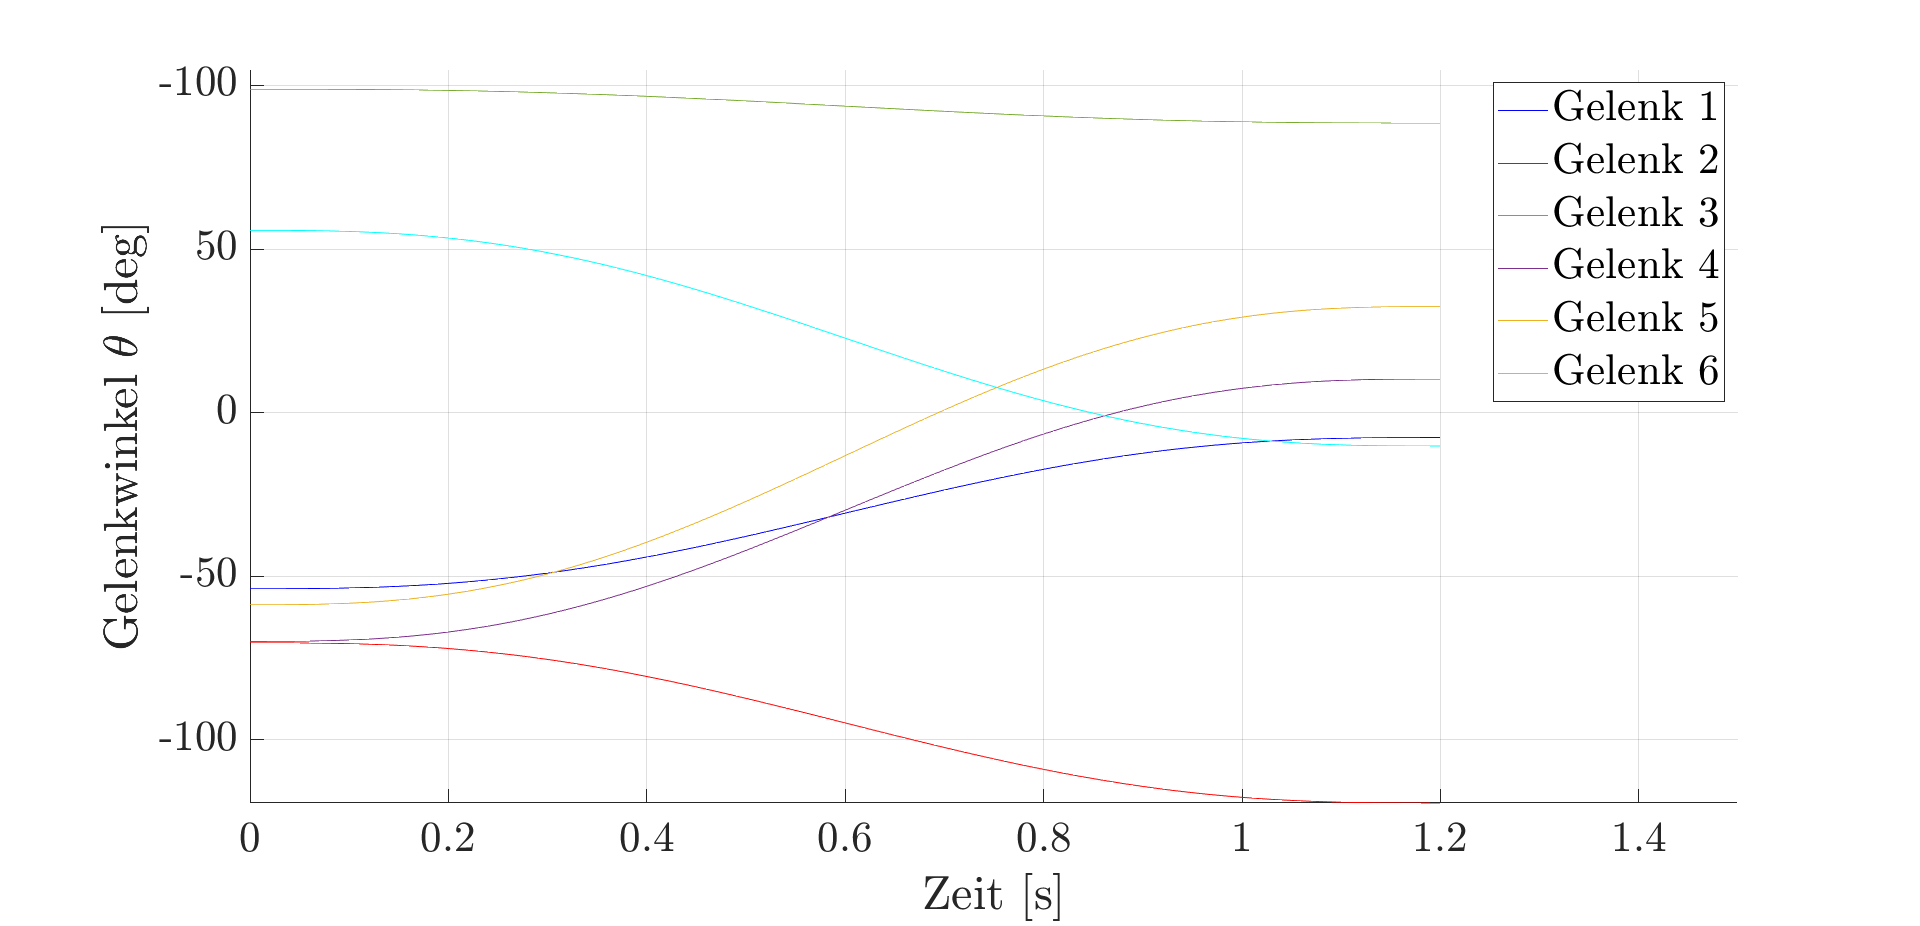
\includegraphics[width=1\linewidth]{images/gelenkwinkel}
	\caption{Gelenkwinkel}
	\label{fig:gelenkwinkel}
\end{figure}
%
\begin{figure}[]
	\centering
	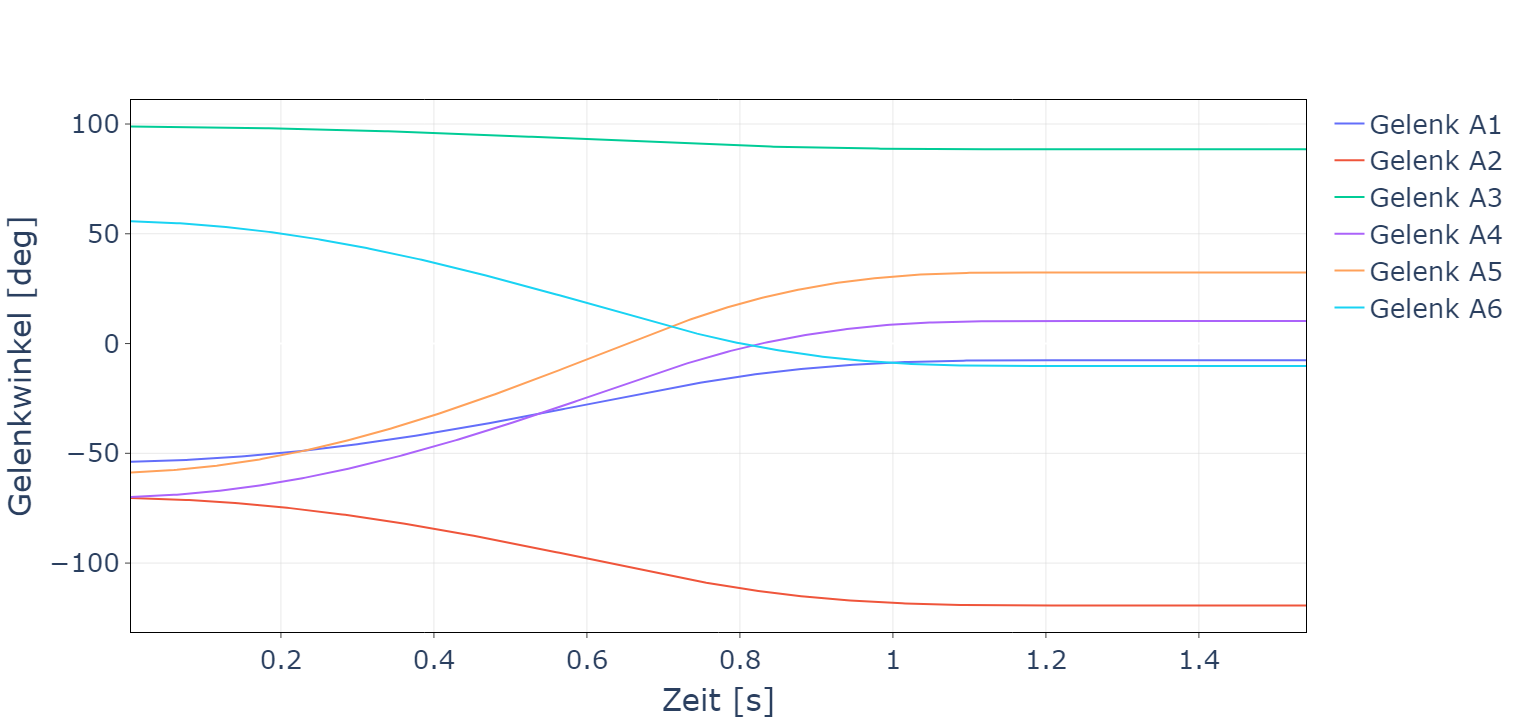
\includegraphics[width=1\linewidth]{images/gelenkwinkel_py}
	\caption{Gelenkwinkel}
	\label{fig:gelenkwinkelpy}
\end{figure}
%
\newpage
\begin{figure}[]
	\centering
	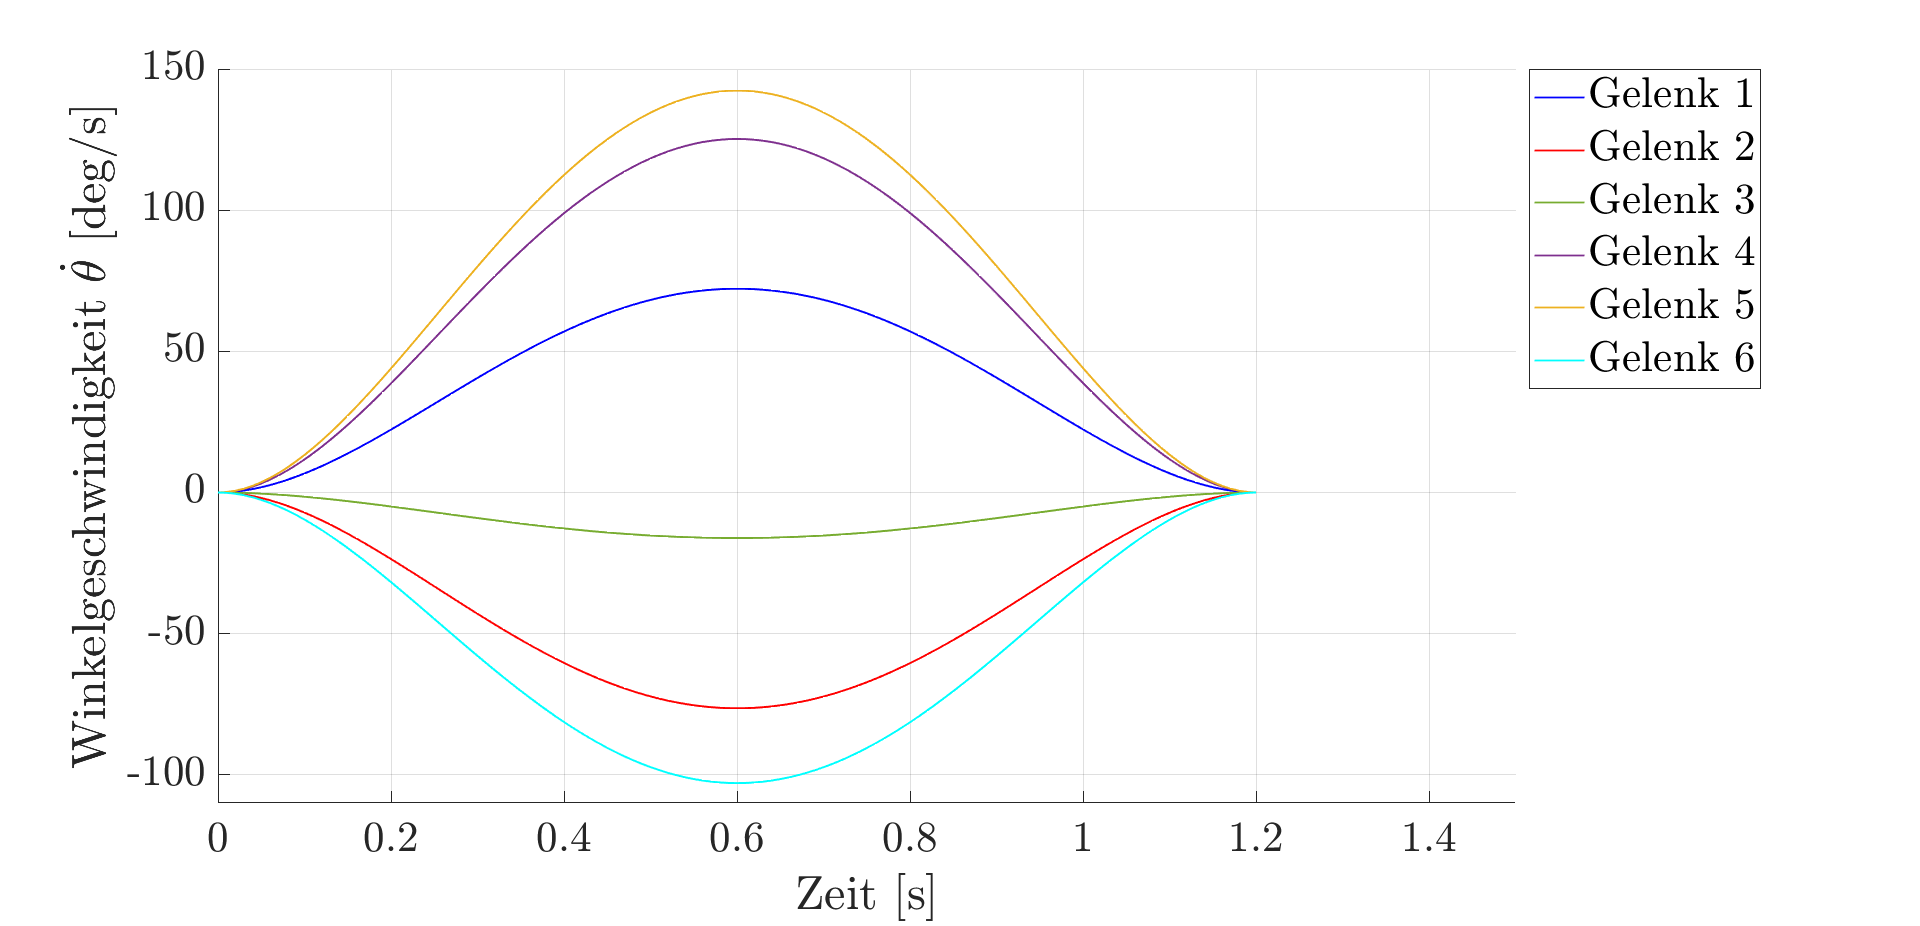
\includegraphics[width=1\linewidth]{images/winkelgeschwindigkeit}
	\caption{Winkelgeschwindigkeit}
	\label{fig:winkelgeschwindigkeit}
\end{figure}
%
\begin{figure}[]
	\centering
	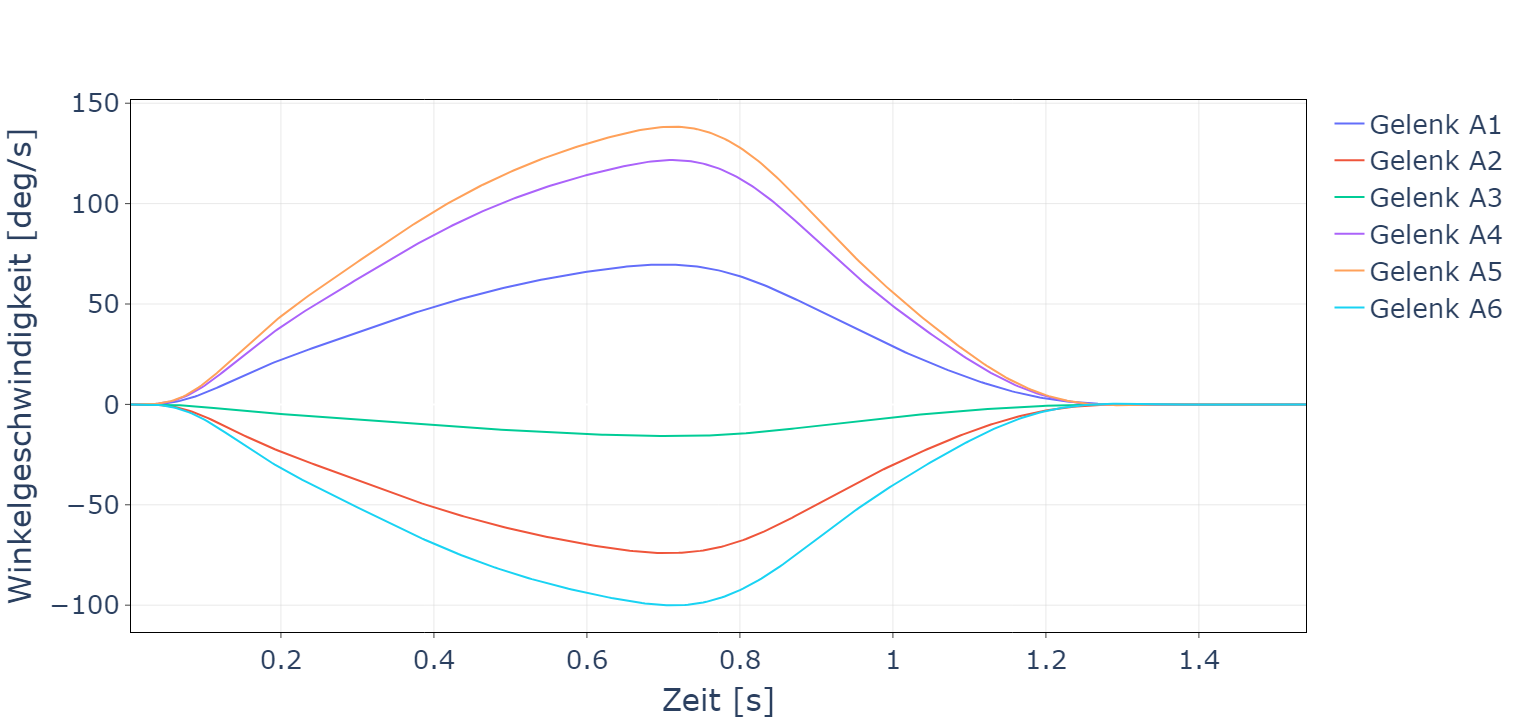
\includegraphics[width=1\linewidth]{images/winkelgeschwindigkeit_py}
	\caption{Winkelgeschwindigkeit}
	\label{fig:winkelgeschwindigkeit_py1}
\end{figure}
%
\newpage
\begin{figure}[]
	\centering
	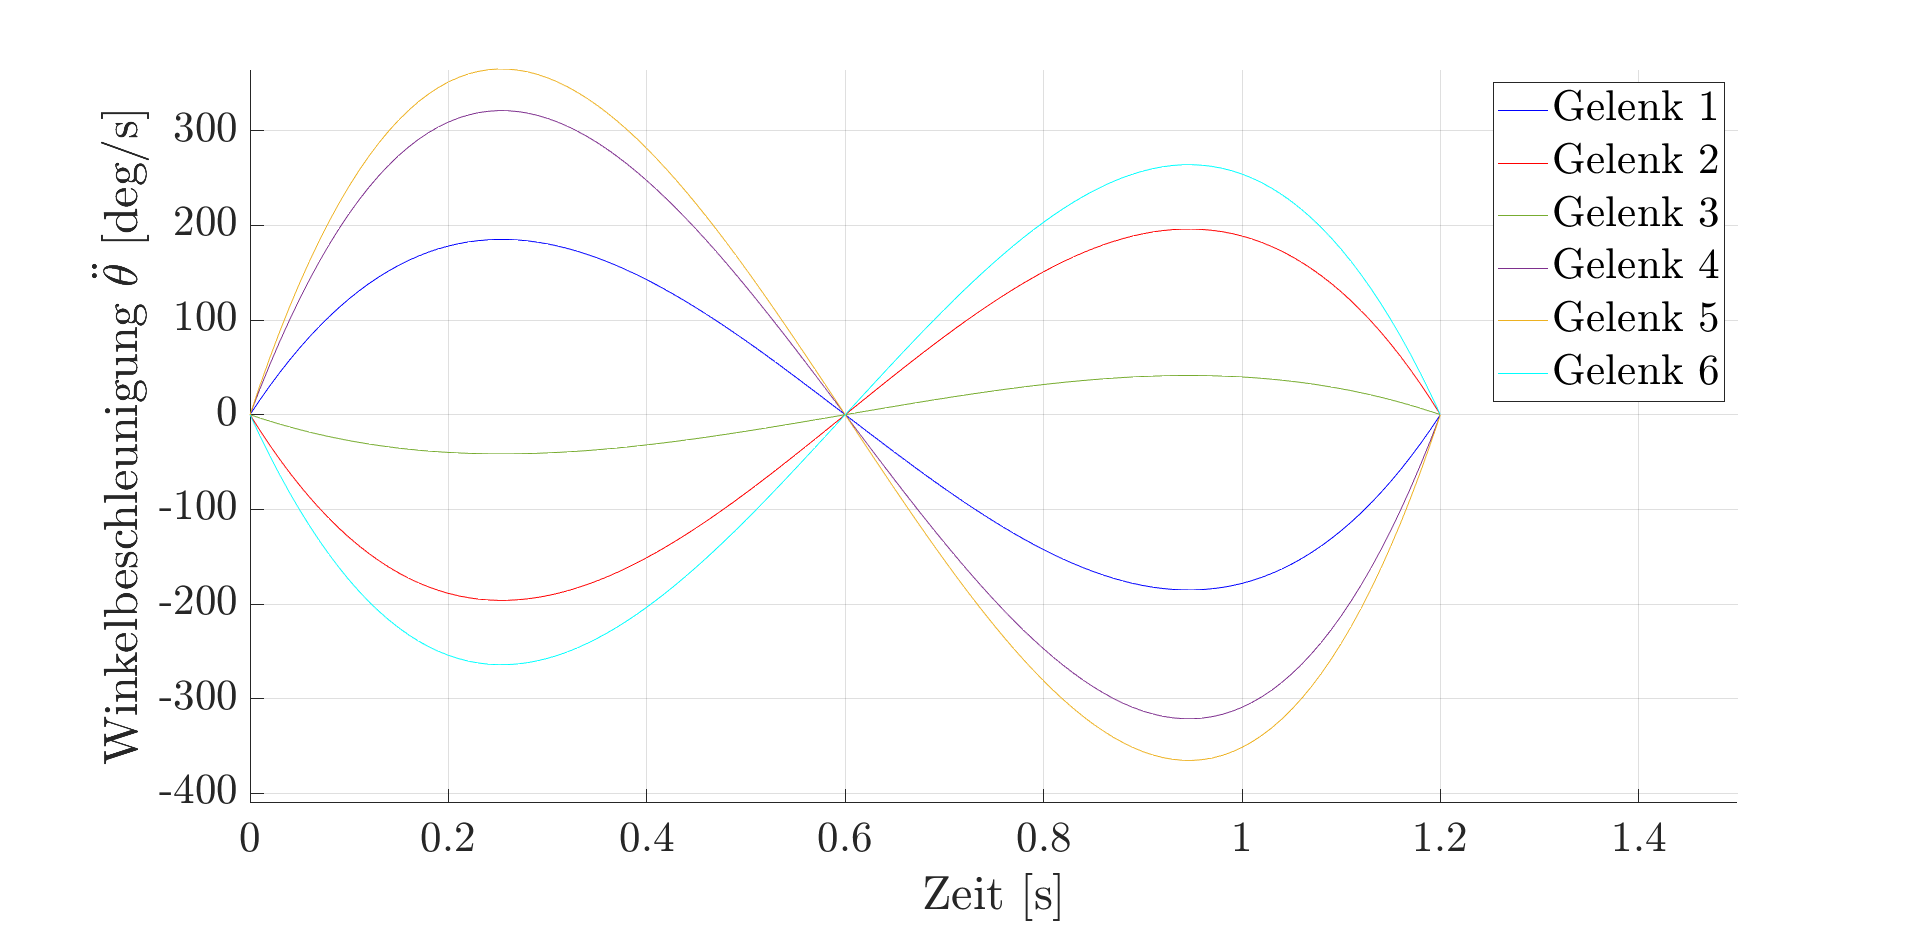
\includegraphics[width=1\linewidth]{images/winkelbeschleunigung}
	\caption{Winkelbeschleunigung}
	\label{fig:winkelbeschleunigung}
\end{figure}
%
\begin{figure}[]
	\centering
	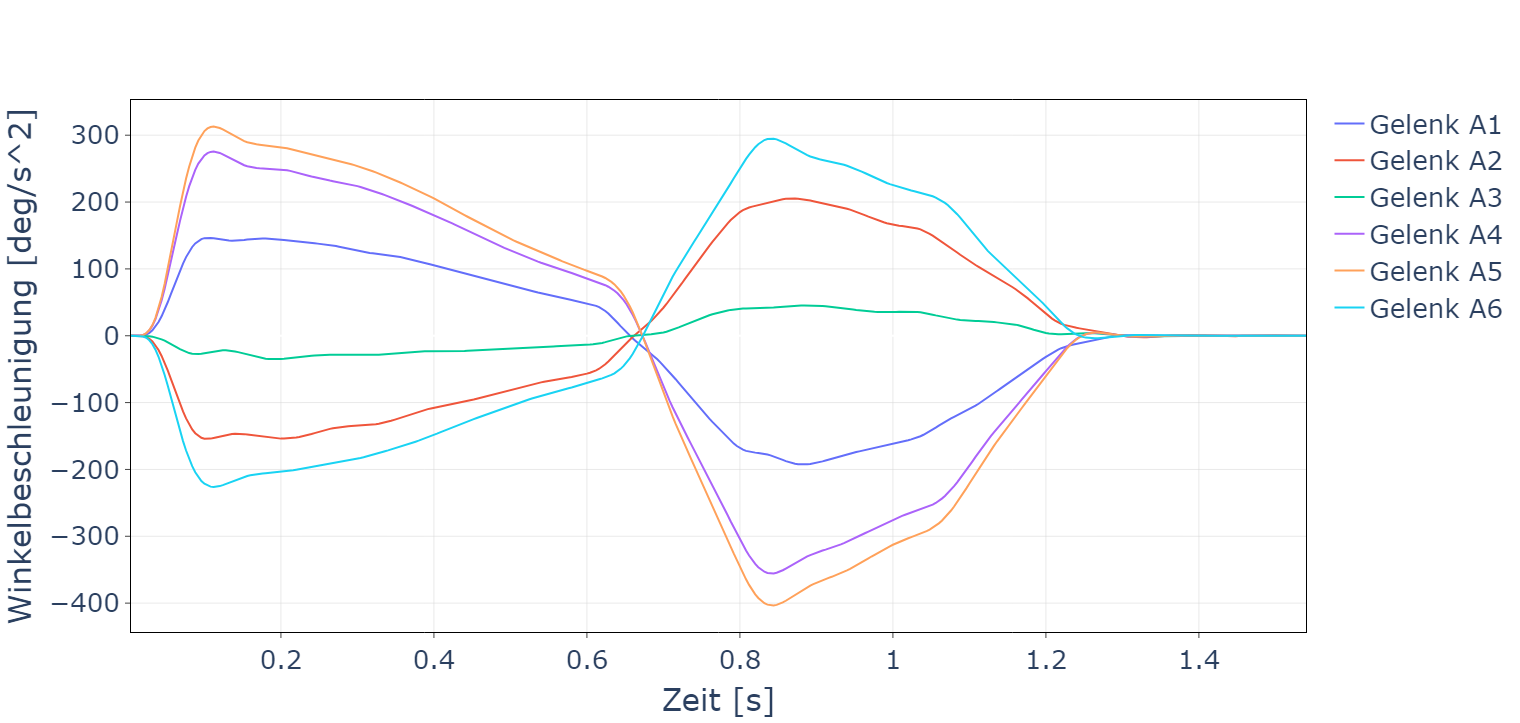
\includegraphics[width=1\linewidth]{images/winkelbeschleunigung_py1}
	\caption{Winkelbeschleunigung}
	\label{fig:winkelbeschleunigung_py}
\end{figure}

\chapter{Validierung des Roboterdynamik-Modells}
\label{sec:modellvalidierung}
\label{cha:modellvalidierung}
%
Unter Berücksichtigung der getroffenen Annahmen wird untersucht, ob das implementierte Modell die Roboterdynamik hinreichend genau simuliert. Dazu werden die simulierten Drehmomente qualitativ und quantitativ mit den gemessenen Werten verglichen
%
\section{Messaufbau}
Als Testumgebung dient eine Roboterzelle in der digitalen Anlauffabrik des Mercedes-Benz Werks Berlin.
%Die Roboterzelle stellt einen von acht Laborbereichen zur Erprobung standardisierter Fertigungstechnologien dar.  
Der abgegrenzte Zellbereich ist mit Sicherheitseinrichtungen zur Gewährleistung der Personen- und Maschinensicherheit ausgestattet.
%sodass ein erheblich minimiertes Unfallrisiko in den Praxisversuchen gewährleistet ist. 
Der Roboter besitzt kein, am Flansch montiertes Werkzeug so dass das Kollisionsrisiko in den Versuchen im Vergleich zu einem Endeffektor (EE) mit komplexen Geometrien geringer ausfällt. Darüber hinaus ist eine signifikante Abweichung von der initialen Bahn durch Anwendung Bahnoptimierung wie in der Auswertung gezeigt nicht zu erwarten. Der Grund dafür hängt mit der Bahnplanung durch die Robotersteuerung zusammen. In der PTP-Bewegungsart berechnet die KR C5 den schnellsten Weg des Tool-Center-Point (TCP) zwischen Start- und Zielpunkt \cite[S.~429]{KSS.2023}. Eine stark abweichende Bahn im kartesischen Raum würde zu einem längeren Weg im Gelenkraum und damit zu einem höheren Energieverbrauch führen \cite[S.~59]{Eggers.2019}.
%5
%Ein Arbeitsgebiet der digitalen Anlauffabrik ist die Auswertung von prozessbezogenen Daten, sodass 
%
Der installierte KUKA KR 210 wird über eine KR C5 angesteuert, welche die KUKA RobotSensorInterface 5.0 (RSI) Technologie unterstützt. RSI ist eine Schnittstelle zur zyklischen Kommunikation zwischen dem Industrieroboter und einem Sensorsystem. Die Robotersteuerung kommuniziert mit dem Sensorsystem über eine echtzeitfähige Netzwerkverbindung. Die Daten werden dabei über das Ethernet UDP/IP-Protokoll \footnote{User Datagram Protocol (UDP) ist ein verbindungsloses Protokoll für den Datenaustausch von Netzwerkteilnehmern~\cite{RSI.2020}.} übertragen ~\cite[S.~11]{RSI.2020}. Der Roboter verfügt damit über eine Schnittstelle zur Aufzeichnung von Bewegungsdaten und den Messwerten interner Messeinrichtungen.  
%
Auf der Robotersteuerung ist daf{\"u}r ein RSI-Kontext zu parametrieren, wobei festgelegt wird, welche Daten an eine festgelegte Ziel-IP-Adresse inkl. Port {\"u}bertragen werden.~\cite[S.~43]{RSI.2020}.  Der Datenaustausch findet unidirektional zwischen zwei Netzwerkteilnehmern statt. Die KR C5 hat die Funktion eines sendenden Clients. Der Empfänger (Notebook) stellt den Server dar. Auf dem Empfänger wird die Ethernet Verbindung mit der definierten IP Adresse eingerichtet. Des Weiteren wird der im RSI Kontext festgelegte UDP-Port freigegeben. Der Port-Zugriff wird auf dem Windows Betriebssystem des Servers über die Programmierschnittstelle (Application Programming Interface(API)) Windows Sockets 2 (Winsock) realisiert \cite{Winsock.2023}. 
%
Der entsprechende RSI-Kontext wird im Initialisierungsschritt des KRL-Programms aktiviert \cite[S.~50]{RSI.2020}. Anschließend werden die Daten der erfassten Winkelverläufe und Drehmomente der einzelnen Gelenke in einem Takt von 4 ms in der American Standard Code for Information Interchange (ASCII) Darstellung an den Server übertragen. Die Daten werden in einem Textfile gespeichert und mithilfe der Skriptsprache Python in die JavaScript Object Notation (JSON) konvertiert, verarbeitet und visualisiert. 
%
Neben den Winkelverläufen werden die Winkelgeschwindigkeit, Winkelbeschleunigung, sowie die mechanische Leistung in den jeweiligen Gelenken benötigt. Da Winkelgeschwindigkeit und Winkelbeschleunigung nicht explizit zur Verfügung stehen, werden sie über den Differenzenquotient, siehe Kapitel \ref{sec:tarjektorie} gebildet. Durch Multiplikation der Winkelgeschwindigkeit mit dem Getriebe-Drehmoment wird der zeitliche Verlauf der mechanischen Leistung berechnet.

\section{Durchführung}
% Temperatur kalt und warm 
%Versuchsbeschreibung
Die Validierung des Modells erfolgt exemplarisch für die in der Tabelle \ref{tab:simu} definierte initiale Trajektorie aus dem Programm $Kleben-Seitenwand$. Die Betriebstemperatur des Roboters wird aufgrund der Vernachlässigung von Reibungseinflüssen im Modell nicht berücksichtigt. Die simulierten, sowie gemessenen Verläufe der Gelenkwinkel, Winkelgeschwindigkeit und Winkelbeschleunigung sind bereits im letzten Kapitel abgedruckt. Die simulierten Drehmomente werden in \ref{fig:taumat} gezeigt. Die gemessenen Werte sind in der Abbildung \ref{fig:tau} dargestellt. In beiden Fällen werden die Drehmomente auf der Getriebeseite betrachtet. Dies erfolgt mit dem Ziel die Zusammenhänge zwischen Drehmoment, Winkelgeschwindigkeit und mechanischer Leistung eindeutig erkennbar abzubilden. Eine Darstellung der Drehmomente auf der Motorseite wird vermieden. Durch Anwendung der Getriebe-Übersetzung ergibt sich eine Änderung des Vorzeichens der Momente in den Gelenken eins, zwei, vier und fünf, wie in Anhang \ref{add:systemparameter} angegeben, so dass die Zusammenhänge nicht ad hoc erkennbar sind.

\section{Auswertung}
Die gemessenen Drehmomente werden im Zeitintervall 0 s bis 1,3 s zu betrachtet. Daten für den Zeitraum $t>1,3~\text{s}$ entfallen auf den Vorgang der Antriebsregelung bis zum Einfallen der Haltebremsen, um den Roboter in Position zu halten. 
\subsection*{Quantitative Auswertung der Drehmomente}
Die simulierten Drehmomente fallen signifikant größer aus als die gemessenen. Der negative Maximalwert von $\tau_2$ liegt in der Simulation bei ca. -12 kNm. Dem gegenüber steht ein gemessener Wert  von ca. -2,8 kNm. Die Differenz wird der Vernachlässigung des Gewichtsausgleichs zugeschrieben. Dieser kompensiert insbesondere den Einfluss der Gewichtskraft nachfolgender Glieder am zweiten Gelenk. Exemplarisch zeigt Abbildung \ref{fig:gewichtskraft} den simulierten Anteil der Gewichtskraft bei Stillstand des Roboters in der Ausgangsstellung $q_{s,i}$ siehe Tabelle \ref{tab:simu}. Für die Drehmomente am zweiten Gelenk ist erkennbar, dass der Anteil der Gewichtskraft von -7743 Nm genau dem  Offset des Drehmoments beim Start der Bewegung entspricht. In der Konsequenz fällt $\tau_2$ im Gütekriterium der Optimierung zu stark ins Gewicht. Daraus wird abgeleitet, dass der Gewichtsausgleich in der Modellbildung zu berücksichtigen ist. 
%
\begin{figure}[tbph]
	\centering
	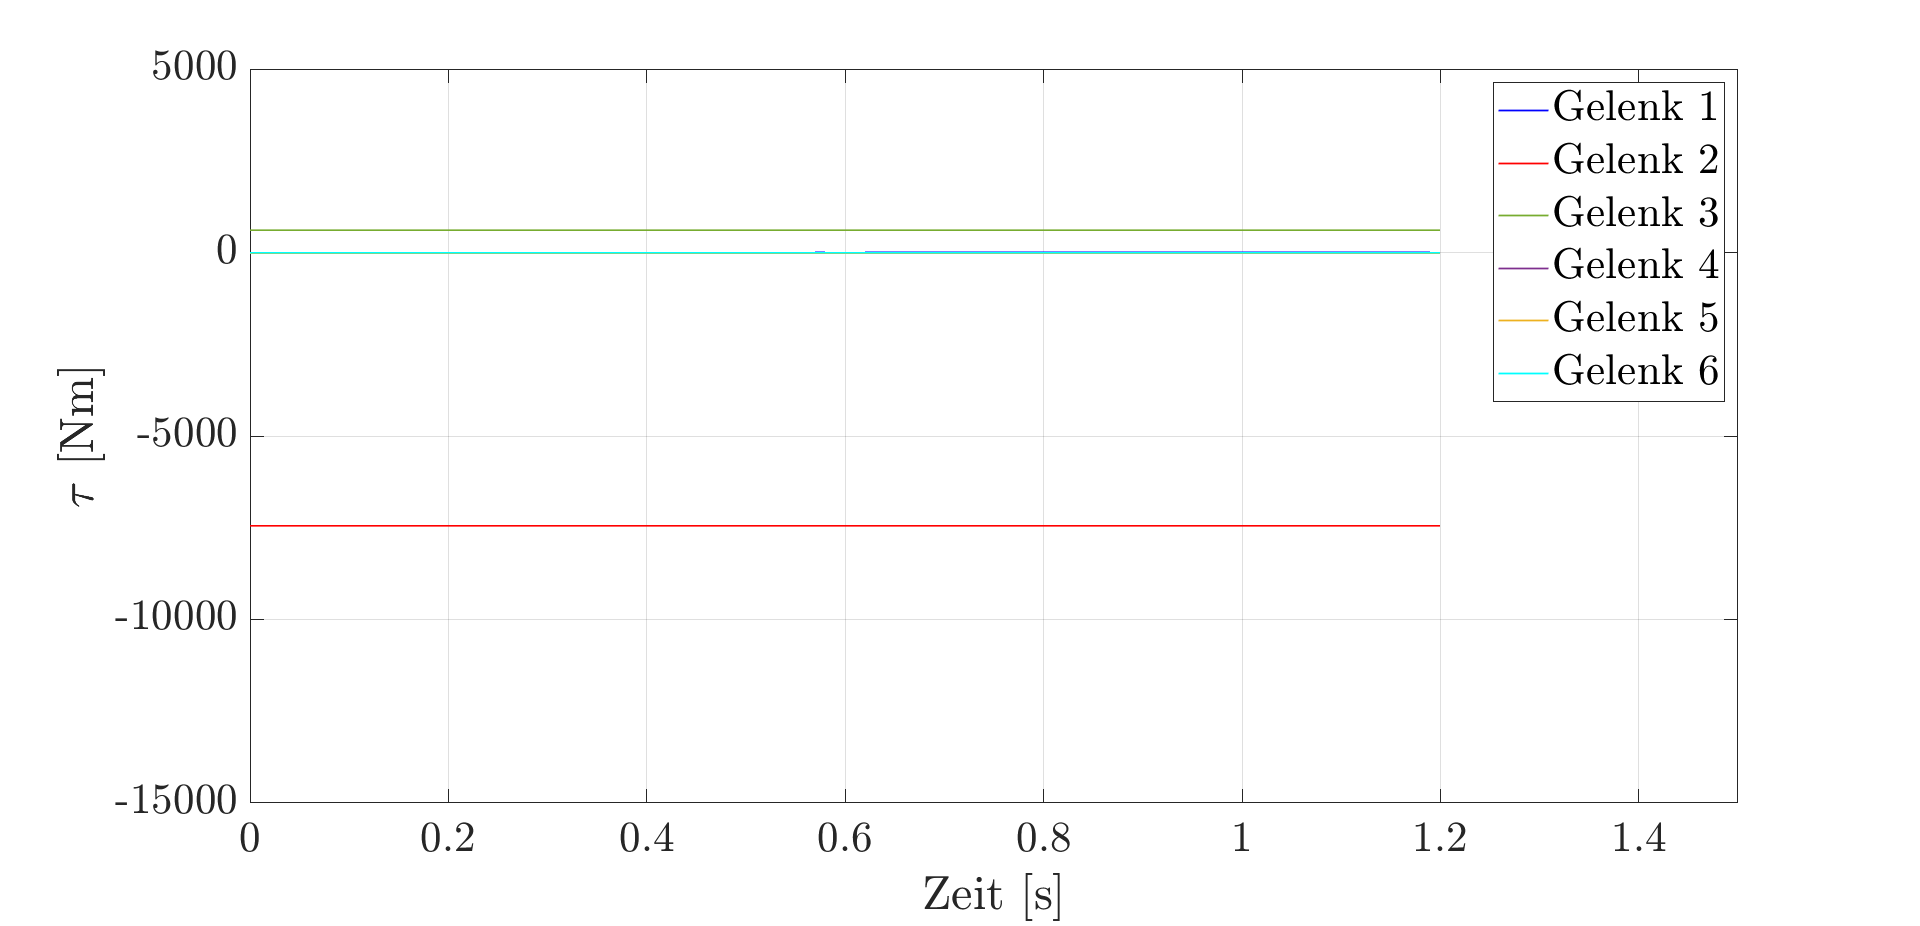
\includegraphics[width=1\linewidth]{images/Gewichtskraft}
	\caption{Anteil der Gewichtskraft an den Drehmomenten in der Startposition}
	\label{fig:gewichtskraft}
\end{figure}
%
%Idealerweise kompensiert der Ausgleichszylinder den Einfluss der Gewichtskraft aller nachfolgenden Glieder im zweiten Gelenk, siehe Abbildung \ref{fig:taumat-fgall}. 
%%
%\begin{figure}[tbph]
%	\centering
%	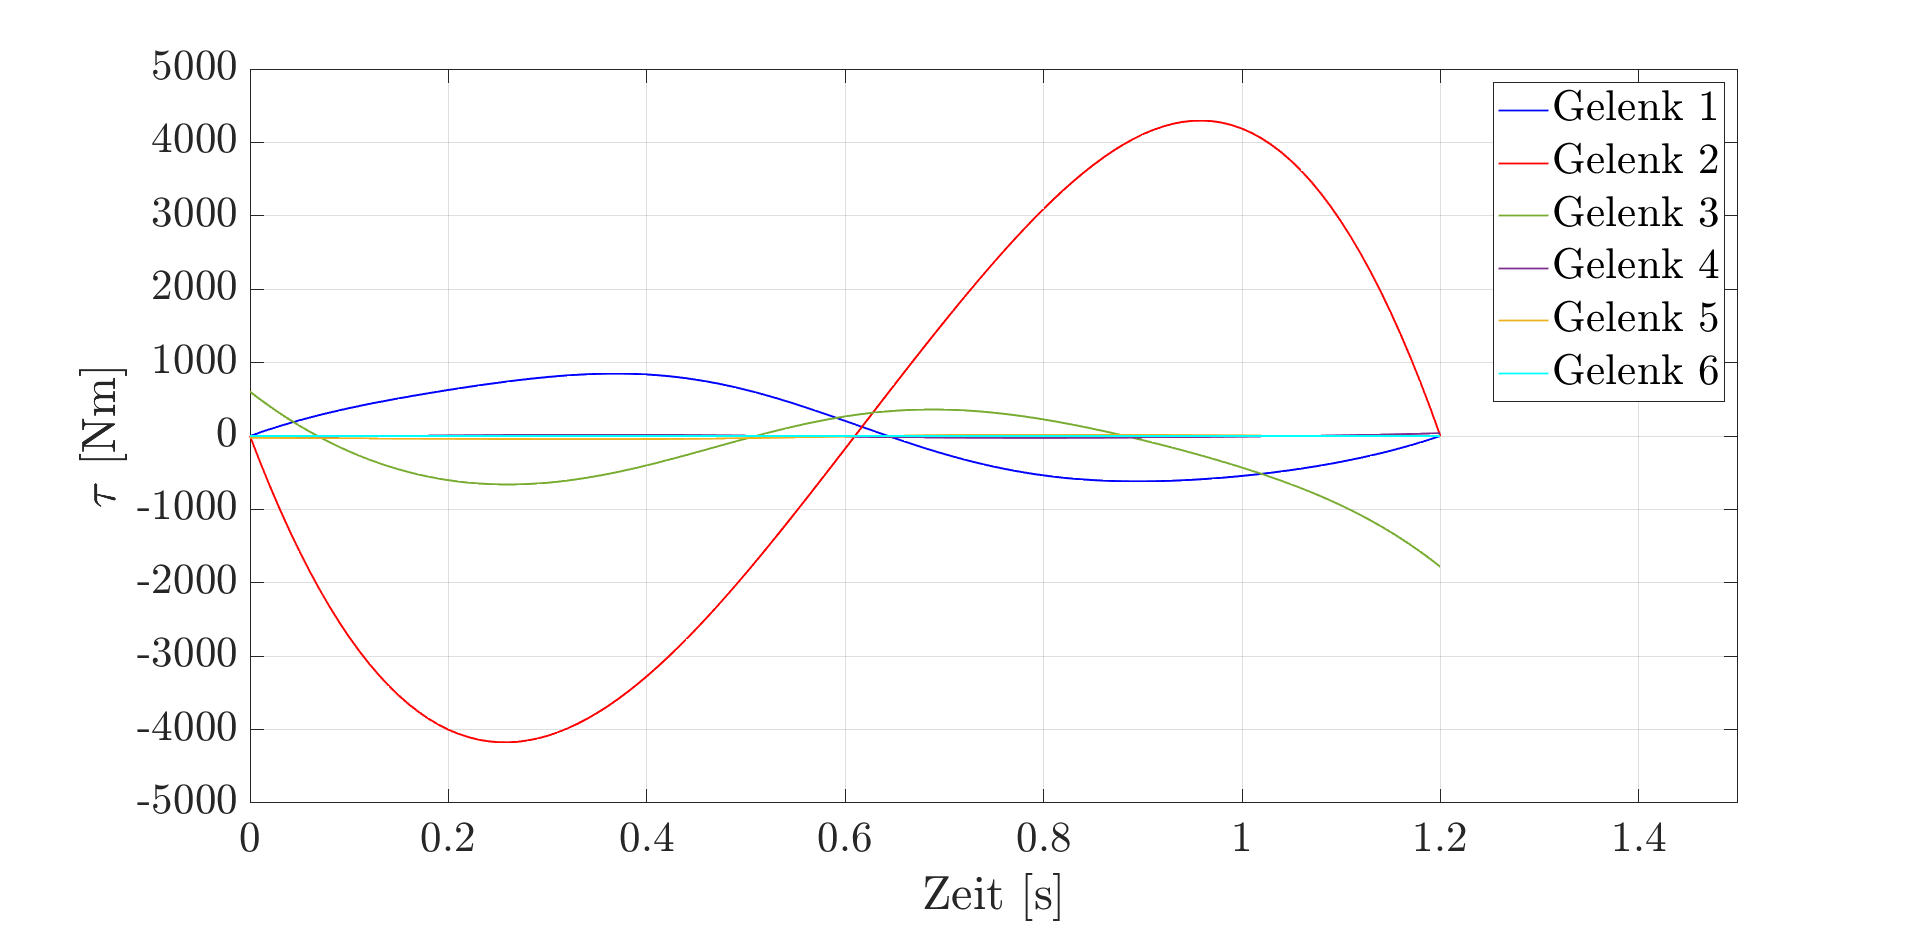
\includegraphics[width=1\linewidth]{images/taumat-fgall}
%	\caption{Drehmomentverlauf simuliert inkl. idealen Gewichtsausgleich}
%	\label{fig:taumat-fgall}
%\end{figure}
%
%Die Idealkompensation bildet jedoch nicht die Realität ab. Dies wird am Leistungsverlauf \ref{fig:p_ideal} gegenüber \ref{fig:p} nachgewiesen. 
%Es wird ein Kompromiss gewählt, bei dem ausschließlich die  Gewichtskraft des zweiten und dritten Verbindungsglieds ausgeglichen wird. 
Der Gewichtsausgleich wurde so gewählt, dass er den Anteils der Gewichtskraft des zweiten und dritten Verbindungsglieds am Drehmoment des zweiten Gelenks ausgleicht. 
Das Roboter-Dynamikmodell wird um die Vorschrift \ref{eqn:submugrav} erweitert.
%
\begin{equation}
	\label{eqn:submugrav}
\bm{\mu}^{i}_{i} = \bm{\mu}^{i}_{i} - {\bm{\mu}^{i}_{i}}_{grav} ~\forall ~i = 2
\end{equation}
%
wobei
%
\begin{equation}
	\label{eqn:mugrav}
	{\bm{\mu}^{i}_{i}}_{grav} = -{\bm{f}^{i}_{i}}_{grav} \times \left( \bm{r}^{i}_{i-1,i} + \bm{r}^{i}_{i,C_i} \right) + \bm{R}^{i}_{i+1} {\bm{\mu}^{i+1}_{i+1}}_{grav} + \bm{R}^{i}_{i+1} {\bm{f}^{i+1}_{i+1}}_{grav} \times \bm{r}^{i}_{i,C_i} ~\forall ~i = 2
\end{equation}
%
\begin{equation}
	\label{eqn:mugrav}
	{\bm{\mu}^{i}_{i}}_{grav} = -{\bm{f}^{i}_{i}}_{grav} \times \left( \bm{r}^{i}_{i-1,i} + \bm{r}^{i}_{i,C_i} \right) ~\forall ~i = 3
\end{equation}
%
\begin{equation}
	\label{eqn:subfgrav}
	{\bm{f}^{i}_{i}}_{grav} = \bm{R}^{i}_{i+1} {\bm{f}^{i+1}_{i+1}}_{grav} + m_i\ddot{\bm{p}}^{i}_{C_i} - {\bm{R}^0_i}^T - m_i \bm{g} ~\forall ~i \in \{2,3\}.
\end{equation}
%
Es folgt ein Drehmomentverlauf gemäß Abbildung \ref{fig:taumat-fg}. 
%
% Quelle Reibung Getriebe
%
\subsection*{Qualitative Auswertung der Drehmomente}
Die Gelenke werden nachfolgend einzeln betrachtet. Für das erste Gelenk weißt der gemessene Drehmomentverlauf einen steileren Anstieg als die simulierten Werte auf. Dieser Anstieg ist äquivalent zum Verlauf der Winkelbeschleunigung im selben Zeitabschnitt, siehe Abbildung \ref{fig:winkelbeschleunigung_py}. Das Maximum der simulierten Werte für das erste Gelenk ist ca. 50 \% kleiner als die gemessenen Werte. In der Ursache wird die Reibung des Getriebes vermutet. Der gemessene Drehmomentverlauf im ersten Gelenk weißt außerdem keinen negativen Anteil auf. Es wird angenommen, dass die Getriebemomente in der Signalaufzeichnung mithilfe von messtechnisch erfassten Motorströmen sowie der Drehmomentkonstanten und der Getriebeübersetzungsfaktoren berechnet werden. Unter der Annahme, dass die Bremsenergie nicht zurückgewonnen wird, sondern über Bremswiderstände dissipiert, entsprechen die gemessenen Werte für $t>0,8~\text{s}$ dem  Abbremsvorgang. Belegt wird dies mit dem übereinstimmenden Verlauf der Winkelgeschwindigkeit, siehe Abbildung \ref{fig:winkelgeschwindigkeit_py1}. Dass der Drehmomentverlauf dem Geschwindigkeitsverlauf dabei um ca. 0,02 s nachläuft, wird den Energie speichernden Induktivitäten der Antriebe zugeschrieben. Für den Drehmomentverlauf im zweiten Gelenk sind ebenfalls steilere Anstiege infolge eines höheren Rucks des realen Roboters festzustellen. Im Verlauf ist das negativen Maximum des simulierten Drehmoments im zweiten Gelenk ca. 2000 Nm größer als das aufgezeichnete Drehmoment des realen Systems. Die Differenz wird dem nur näherungsweise modellierten Gewichtsausgleich zugeschrieben. Aufgrund der kinematischen Kopplung wirkt der Einfluss des Gewichtsausgleichs am realen Roboter indirekt auch auf das dritte Gelenk womit der Offset zu Beginn der Bewegung erklärt wird. Dass die Größenordnung des Drehmoments im dritten Gelenk nicht erreicht wird, wird der Vernachlässigung der Stator-Massen von für die Motoren vier und fünf, der Rotor-Trägheit des dritten Motors, sowie und der Steifigkeit, Masse des Schlauchpakets zugeschrieben. Mit einem Gewicht von 65,3 kg ohne elektrische Leitungen steht die Masse des Schlauchpakets, gemäß CAD-Modell mindestens im Verhältnis 1:5 zur Masse des dritten Verbindungsglieds. Daraus folgt insbesondere eine zusätzliche Massenträgheit, sowie die Verschiebung des Masseschwerpunkts, unter der Annahme, dass die Hardware ausschließlich am dritten Verbindungsglied befestigt ist. Aufgrund fehlender Daten entfällt eine Berücksichtigung des Schlauchpakets. Des Weiteren wird für das Drehmoment im dritten Gelenk sowie die Drehmomente in allen nachfolgenden Gelenken die Vernachlässigung  der Reibungseffekte als Ursache für die erkennbare Abweichung gegenüber den Messdaten vermutet. 
%
\begin{figure}[tbph]
	\centering
	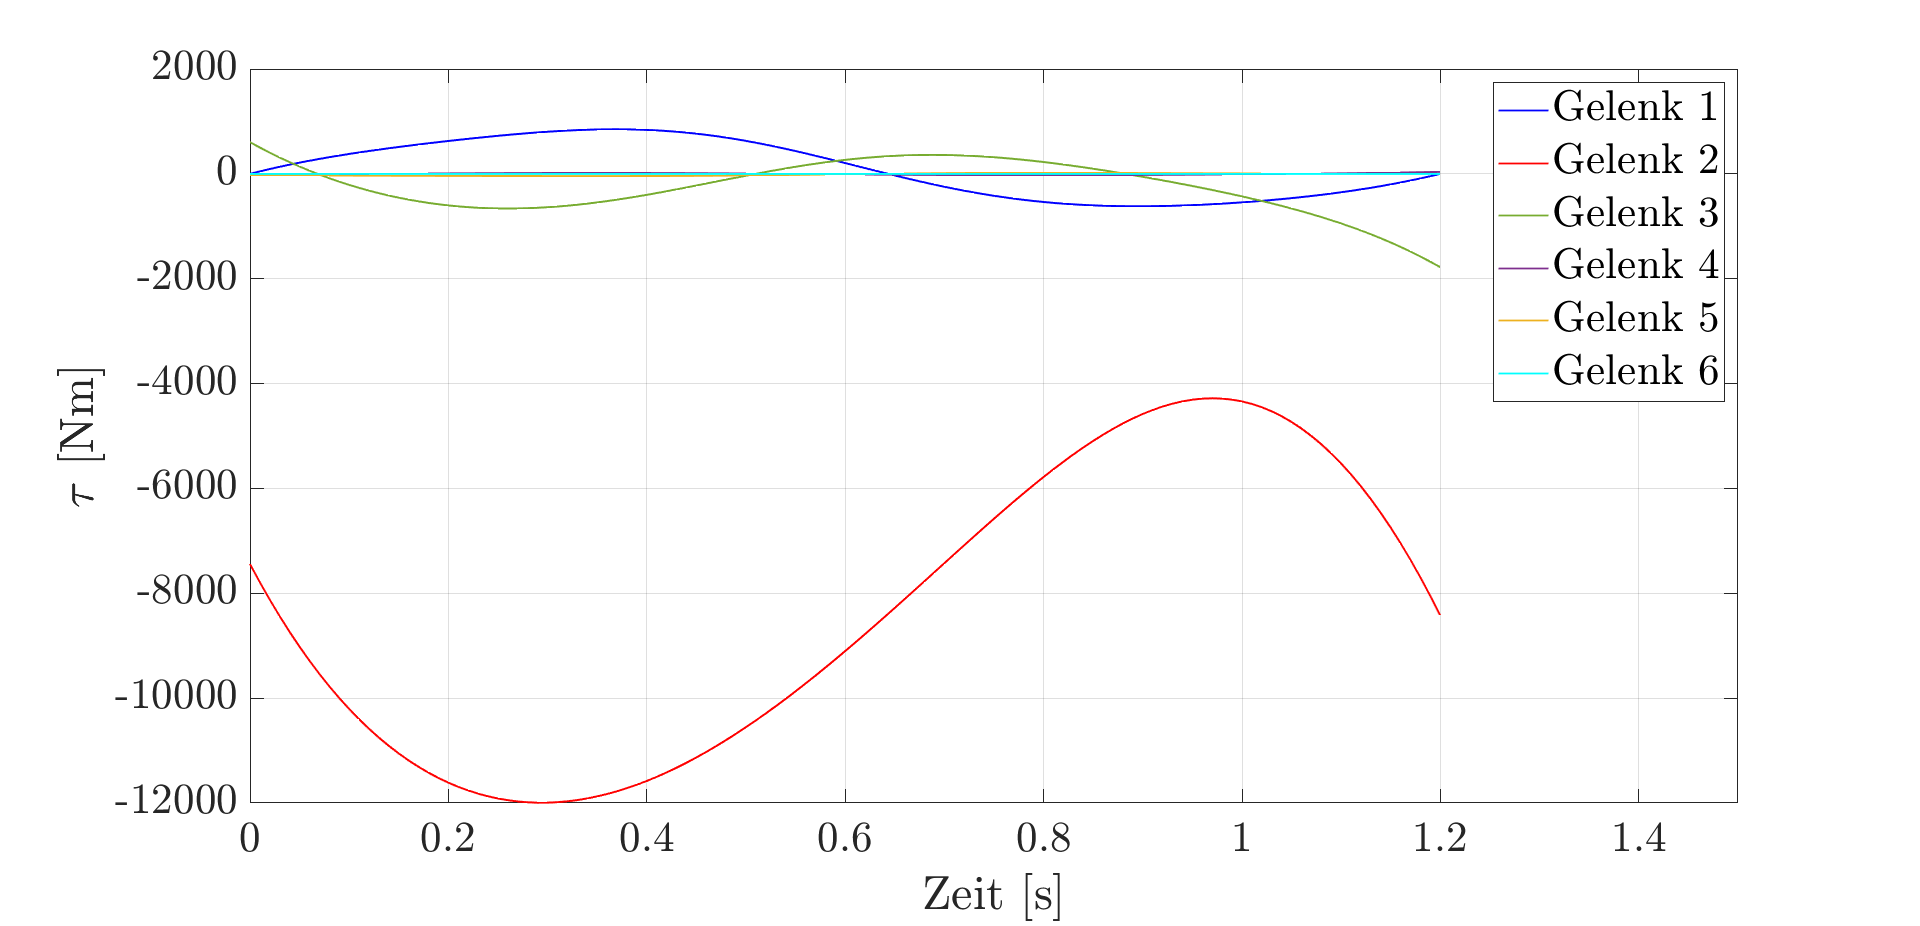
\includegraphics[width=1\linewidth]{images/taumat}
	\caption{Drehmomentverlauf simuliert ohne Gewichtsausgleich}
	\label{fig:taumat}
\end{figure}
%
\begin{figure}[tbph]
	\centering
	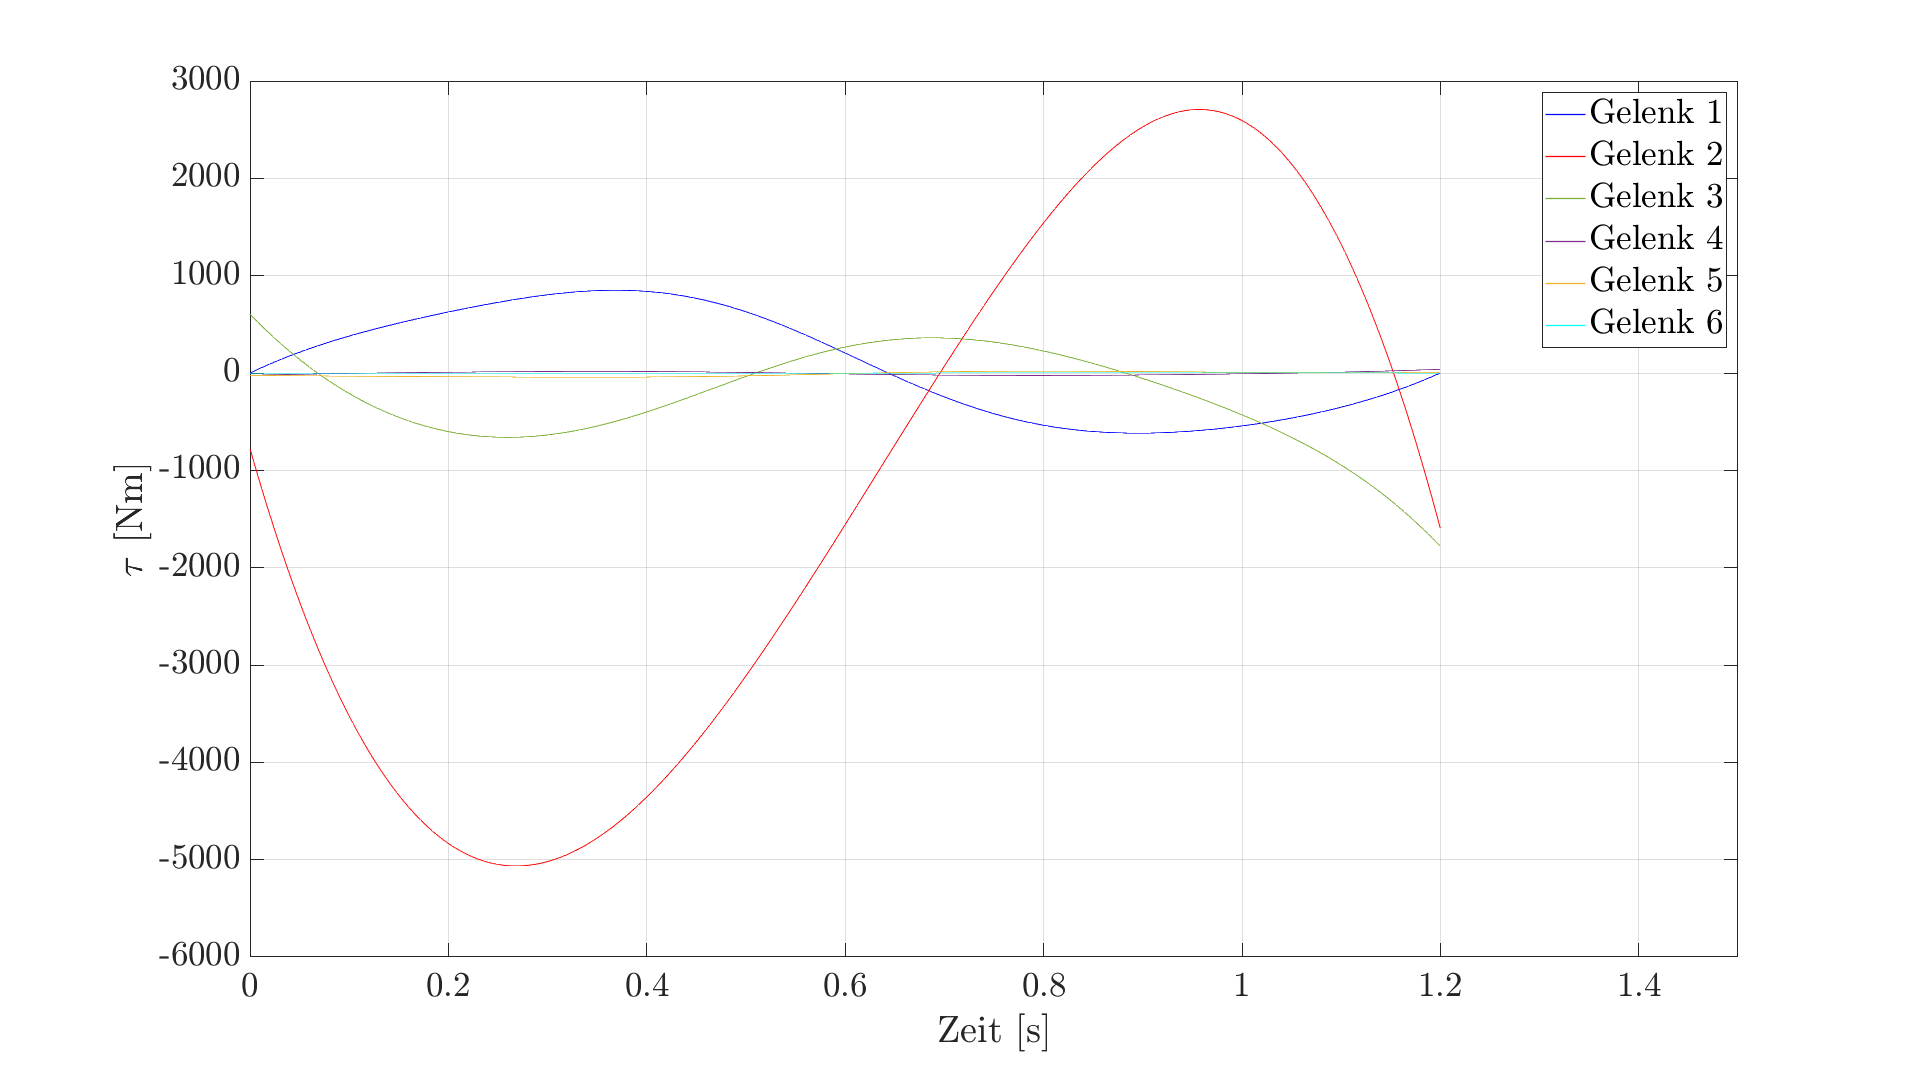
\includegraphics[width=0.9\linewidth]{images/taumat-fg}
	\caption{Drehmomentverlauf simuliert inkl. näherungsweise modellierten Gewichtsausgleich}
	\label{fig:taumat-fg}
\end{figure}
%
\begin{figure}[tbph]
	\centering
	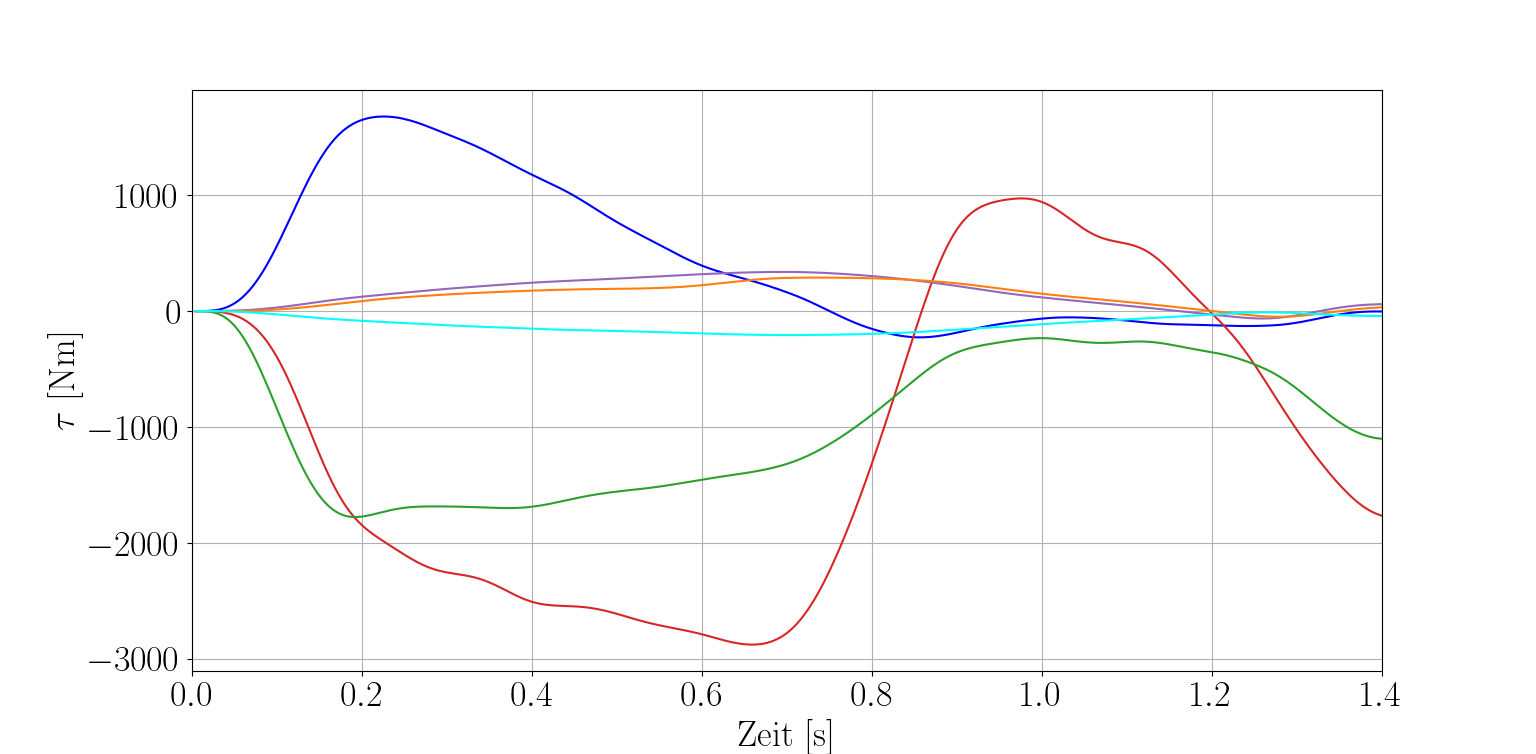
\includegraphics[width=1\linewidth]{images/tau}
	\caption{Drehmomentverlauf gemessen}
	\label{fig:tau}
\end{figure}
%
\subsection*{Auswertung der mechanischen Leistung}
Die simulierten Leistungsdaten des ersten Gelenks stimmen in etwa mit den Werten überein, die auf der Grundlage der RSI Daten berechnet wurden. Der simulierte Verlauf der mechanischen Leistung für das zweite Gelenk weist einen ähnlichen Verlauf wie die messtechnisch erfassten Werte auf. Der Nulldurchgang der gemessenen Leistungskurve ist um 1,3 Sekunden nach rechts verschoben.  Dies lässt sich unter Berücksichtigung der RSI-Daten zur Winkelbeschleunigung in Abbildung \ref{fig:winkelbeschleunigung_py} auf die kürzere Abbremsdauer des realen Roboters gegenüber der im Modell implementierten Bahnplanung  zurückführen. In der gezeigten Bewegung wird die mechanische Leistung in den anderen Antrieben nicht durch das Modell abgebildet. Infolgedessen liegt der Schwerpunkt der Optimierung auf der Anpassung der Roboterkonfiguration zugunsten des Drehmoments im zweiten Gelenk. 
%
\begin{figure}[tbph]
	\centering
	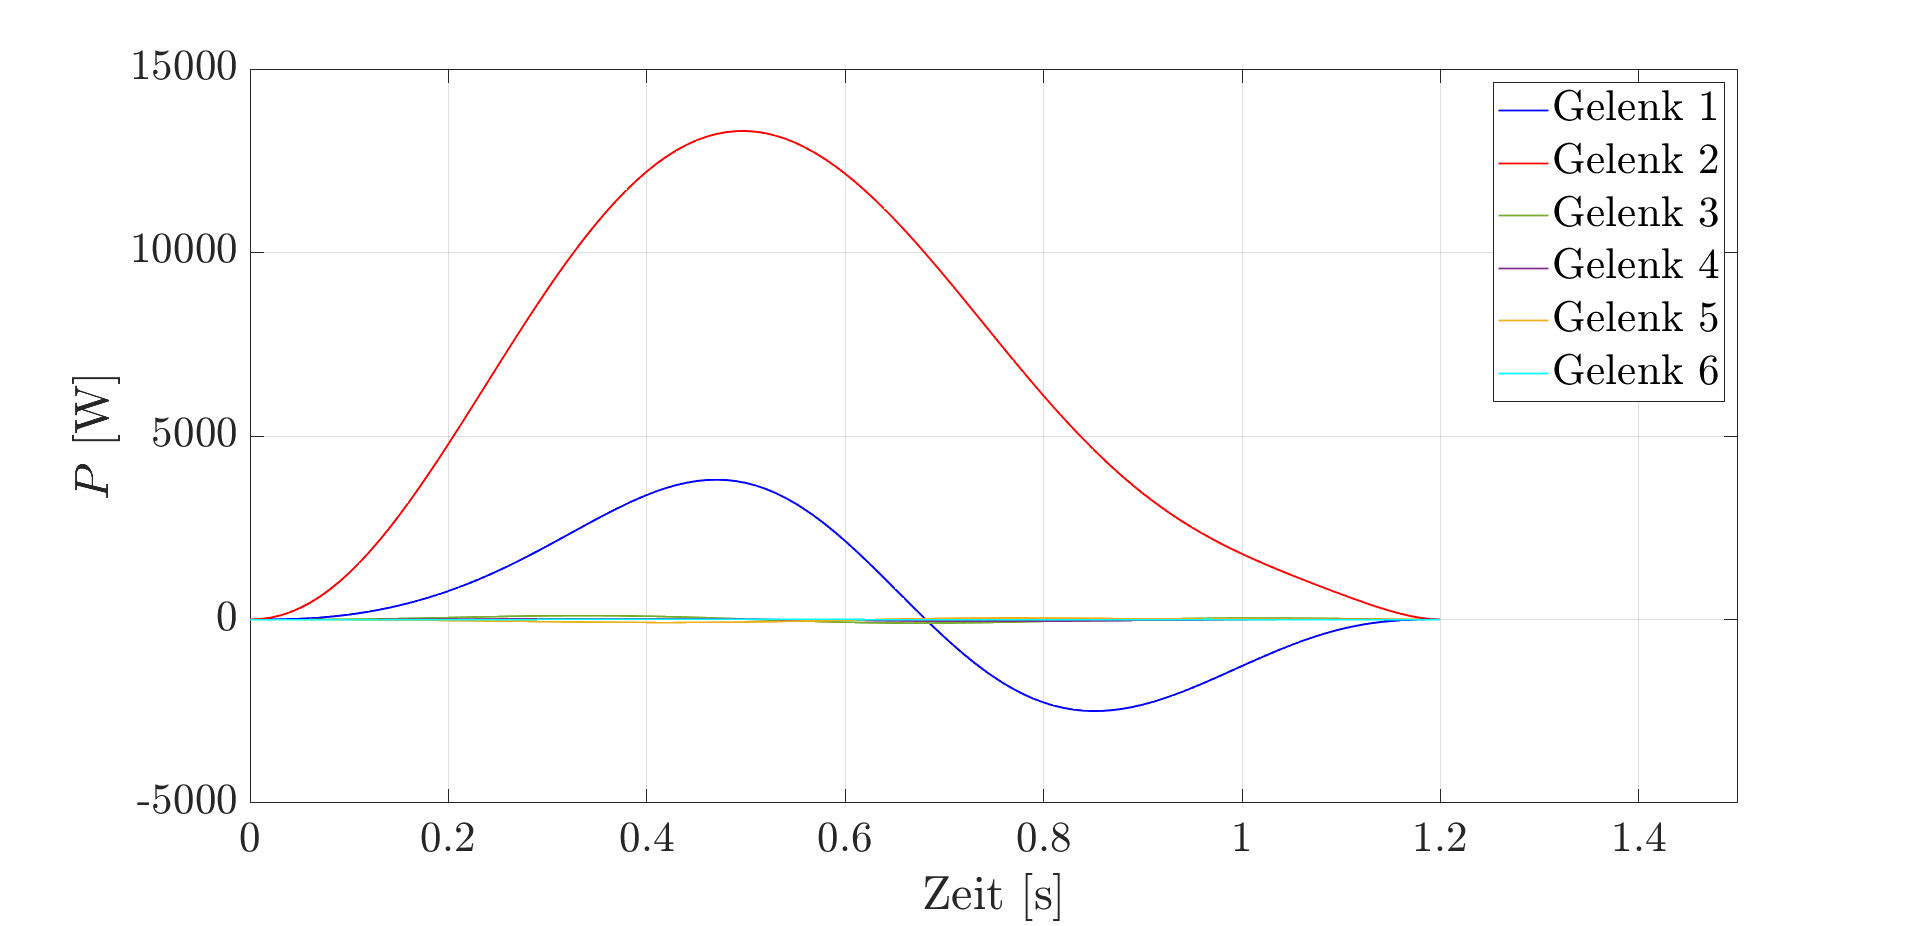
\includegraphics[width=1\linewidth]{images/pmat}
	\caption{mechanische Leistung simuliert}
	\label{fig:pmat}
\end{figure}
%
\begin{figure}[tbph]
	\centering
	\includegraphics[width=1\linewidth]{images/p}
	\caption{mechanische Leistung gemessen}
	\label{fig:p}
\end{figure}
%
\subsection*{Schlussfolgerung}
Es wurde die Qualität eines Modells zur Simulation der mechanischen Leistungsaufnahme des Roboters für eine Bewegung mit der Start- und Zielkonfiguration gemäß Tabelle \ref{tab:simu} untersucht. Die ausgewählte Bahn entspricht dem Verfahrweg des Roboters vom letzten Prozesspunkt zur Grundstellung im Fertigungsprogramm $Kleben-Seitenwand$. Aufgrund des hohen Anteils der gemessenen sowie simulierten mechanischen Leistung für das zweite Gelenk im Vergleich zu den anderen Gelenken wird das größte Optimierungspotenzial im Modell berücksichtigt. Für die untersuchte Bewegung erfüllt das Modell den Zweck der Zielfunktionsberechnung zur Optimierung der ausgewählten Bewegungsbahn.
%
\chapter{Bahnoptimierung}
%\cite{Eggers.2019}
%\cite{Engelke.2008}
%\cite{Ziaukas.2017}
%\cite{Hansen.2012}
%\cite{Spong.2020}
%
\section{Definition des Optimierungsproblems}
Gegenstand der Optimierung ist die Minimierung des Energieverbrauchs eines KR210 R2700-2 Industrieroboters entlang einer Bewegungsbahn. Im Ziel der Arbeit ist festgelegt, den Ansatz möglichst praktikabel für die Automobilproduktion zu gestalten. Dazu wird der Begriff der Bewegungsbahn weiter eingegrenzt. Es wird unterschieden zwischen prozessbezogenen Bewegungen, z.B. entlang einer Schweißnaht oder Klebebahn, und nicht-prozessbezogenen Bewegungen, z.B. das Anfahren einer Vorposition oder der Home-Position in der Bewegungsart PTP. Im Folgenden werden explizit nicht prozessrelevante Trajektorien betrachtet. Der Ansatz basiert auf der geometrischen Anpassung  der Bewegungsbahn durch einen zu optimierenden Parametervektor $\bm{q}_{v}$. Dieser umfasst die Gelenkwinkel des, nach der Hälfte der Bewegungsdauer definierten Via-Punkts \cite[S~532~ f.]{Ziaukas.2017}.
%
\begin{equation}
	\bm{q}_{v} = [q_{v,1},...,q_{v,6}]^T 
\end{equation}
%
Der Startwert jedes Via-Punkts wird auf der Hälfte der Winkelposition zwischen dem Start- und Zielpunkt definiert.
\begin{equation}
	q_{v,i,Start} = \dfrac{q_{s,i}+q_{e,i}}{2}
\end{equation}
Die Minimierung der Leistungsaufnahme basiert auf der konfigurationsabhängigen Reduktion der Massenträgheitsmomente in $\bm{M}(\bm{q})$, so dass bei gleichbleibender Winkelbeschleunigung die Drehmomente in den Gelenken reduziert werden \cite[S.~531]{Ziaukas.2017}. Das Optimierungsproblem besteht darin, den Parametervektor zu identifizieren, für den die minimale Zielfunktion erreicht wird.
%\begin{equation}
%	\bm{q}_{v,opt} = \argminA_{\bm{q}_{v}} J_{P_{zu}}(\bm{q}_{v}).
%\end{equation}
%
\begin{equation}
	\argminA_{\bm{q}_{v}} J(\bm{q}_{v}) = \{\bm{q}_{v} \mid J(\bm{q}_{v}) = \min_{\bm{q}_{v,opt}} J(\bm{q}_{v,opt})\}.
\end{equation}
%
\section{Zielfunktion}
Für die Definition der Zielfunktion wird angenommen, dass die generatorisch erzeugte Leistung während des Abbremsvorgangs über Bremswiderstände dissipiert. Zur Identifizierung des Optimums werden die Zielfunktionen \ref{eqn:torque} \cite[S-~1]{Hansen.2012} und \ref{eqn:emech} \cite[S.~57]{Eggers.2019} aufgestellt. Die Integrationsgrenzen $t_s$ und $t_e$ entsprechen dem Start- bzw. Zielzeitpunkt. Der Ausdruck \ref{eqn:torque} erzielt durch Quadrieren den Vorteil, dass hohe Drehmomente stärker gewichtet werden.
%
\begin{equation}
	\label{eqn:torque}
	J_{\tau}(\bm{q}_{v}) = \frac{1}{2}\int_{ts}^{te}\sum_{i=1}^{n}\left|\tau_i(t)\right|^2~dt
\end{equation}
%
Von einem Vorschlag der Zielfunktion \ref{eqn:emechges} \cite[S.~1216]{Saravanan.2008} wird Abstand genommen, da hierbei die generatorisch umgewandelte Leistung während des Abbremsvorgangs als aufgenommene Leistung der Verbraucher bewertet wird. 
%
\begin{equation}
	\label{eqn:emechges}
	J_{P_{mech_{ges}}}(\bm{q}_{v}) = \int_{ts}^{te}\sum_{i=1}^{n}\left|\tau_i(t)\dot{q_i}\right|^2~dt
\end{equation}
%
Die Zielfunktion \ref{eqn:emech} entspricht dem physikalischen Ausdruck der verrichteten Arbeit mit positiven Vorzeichen. Infolgedessen wird ausschließlich die, motorisch aufgenommene, mechanische Leistung berücksichtigt. 
%
\begin{equation}
	\label{eqn:emech}
	J_{P_{mech_{zu}}}
	(\bm{q}_{v}) 
	= E_{mech_{+}}(\bm{q}_{v}) 
	=\int_{ts}^{te}P_{mech_{zu}}(\bm{q}_{v},t)~dt
\end{equation}
%
Die numerische Implementierung der Zielfunktion in  MATLAB\textsuperscript{\textregistered} entspricht der Gleichung  \ref{eqn:numerischezielfunktion}. Die Schrittweite ist in Anlehnung an die Abtastung der Messeinrichtung  mit $\Delta t = 0.004 \text{s}$ festgelegt. Die Anzahl der Schritte $m$  wird gemäß $(t_s-t_e)/\Delta t$ berechnet.
%
\begin{equation}
	\label{eqn:numerischezielfunktion}
	J_{P_{mech_{zu}}}
	(\bm{q}_{v}) 
	= E_{mech_{+}}(\bm{q}_{v}) 
	= \sum_{k=1}^{m} P_{mech_{zu}}(\bm{q}_{v},t)~\Delta t
\end{equation}
%
\section{Nebenbedingungen}
Die Verfahrzeit bleibt gegenüber der Initialbahn konstant und wird durch den Zielzeitpunkt $t_e$ vorgegeben. 
%Eine Anpassung der Variablen für die maximale relative Geschwindigkeit $vel axis[i]$ und Maximalbeschleunigung $acc axis[i]$ im KRL Programm siehe \cite[S.~532]{Ziaukas.2017} erfolgt nicht.
In \cite[S.~40]{Eggers.2019} bzw. \cite[S.~5]{Hansen.2012} werden die Gelenkwinkel der energieoptimalen Bewegungsbahn in der Robotersteuerung über einen Software-in-the-Loop (SiL) Ansatz berechnet. Dadurch ist die Einhaltung von Drehmoment-, Gelenkwinkel-, Geschwindigkeit- und Beschleunigungsgrenzen entsprechend der Gleichungen \ref{eqn:conpos},\ref{eqn:convel}, \ref{eqn:conacc} und \ref{eqn:contau} gewährleistet. 
%
\begin{equation}
	\label{eqn:conpos}
	q_{i,min} \leq q_{i}(t) \leq q_{i,max}  ~\forall~ i \in \{1,2,3,4,5,6\}
\end{equation}
%
\begin{equation}
	\label{eqn:convel}
	\dot{q}_{i,min} \leq \dot{q}_{i}(t) \leq \dot{q}_{i,max}  ~\forall~ i \in \{1,2,3,4,5,6\}
\end{equation}
%
\begin{equation}
	\label{eqn:conacc}
	\ddot{q}_{i,min} \leq \ddot{q}_{i}(t) \leq \ddot{q}_{i,max}  ~\forall~ i \in \{1,2,3,4,5,6\}
\end{equation}
%
\begin{equation}
	\label{eqn:contau}
	\tau_{i,min} \leq \tau_{i}(t) \leq \tau_{i,max}  ~\forall~ i \in \{1,2,3,4,5,6\}
\end{equation}
%
In der vorliegenden Arbeit sind als Nebenbedingungen ausschließlich die Grenzen der Gelenkwinkel $q_{v,i}$ im Via-Punkt definiert. Die Formulierung zielt darauf ab, dass die optimierte Bewegungsbahn nicht signifikant von der Initialbahn abweicht \cite[S.~5]{Hansen.2012}.
\begin{equation}
	q_{v,i} \in [q_{i,min};q_{i,max}] ~\forall~ i \in \{1,2,3,4,5,6\}
\end{equation}
Grenzwerte für die Drehmomente, Winkelgeschwindigkeiten und Winkelbeschleunigungen werden nicht explizit formuliert.  Im Anschluss an die Optimierung erfolgt eine manuelle Überprüfung der Verläufe.
%
\section{Solver- und Optimierungsalgorithmus}
%todo Solver und Optimierungsalgorithmus
%
\section{Durchführung und Auswertung der Optimierungsergebnisse}
Die Untersuchung verfolgt den Anspruch, dass die identifizierten Einsparungen über das Laborumfeld hinaus in der industriellen Praxis realisiert werden können. Dazu wird eine Bewegung der Bewegungsart PTP betrachtet, die in nahezu jedem Programm den Verfahrweg nach Programmende in die Grundstellung abbildet. Exemplarisch wird die Fahrt vom letzten Prozesspunkt zurück in die Grundstellung im Fertigungsprogramm  $Kleben-Seitenwand$  optimiert. Neben der Energieeinsparung wird auch die Verfahrzeit des Roboters auf der neuen Bewegungsbahn analysiert.
% todo OPtimierungsprocedere
% Auswertung

Die identifizierten, energieoptimalen Via-Punkte sind in der Tabelle \ref{tab:optviapunkte} aufgeführt. Auffällig ist, dass für $q_{v,3}$ und $q_{v,4}$ die obere Grenze aktiv ist, sowie für $q_{v,6}$ die untere Grenze d. h. der Gelenkwinkel im Via-Punkt liegt auf dem selben Wert wie der Gelenkwinkel im Start- bzw. Zielpunkt. Für den Gelenkwinkel $q_{v,5}$ wird festgehalten, dass dieser auffällig nah am unteren Grenzwert liegt. Daraus folgt, dass die berechnete Trajektorie für die Gelenkwinkel drei, vier und sechs Werte außerhalb des Intervalls $[q_{i,s};q_{i,e}] ~\forall~ i \in \{3,4,5,6\}$ annimmt. 
\\
\begin{table}
	\centering
	\begin{tabular}{|l|l|l|}
		\hline
		Startwert Gelenkwinkel&  Zielwert Gelenkwinkel&  Via-Punkte\\
		\hline
		$q_{s,1} = -53,8$			&  $q_{e,1} = -7,6^{\circ}$  		&$q_{v,1} = -25^{\circ}$  \\
		\hline
		$q_{s,2} = -70,3^{\circ}$	&  $q_{e,2} = -119,3^{\circ}$    	&$q_{v,2} = -96,1^{\circ}$  \\
		\hline
		$q_{s,3} = 98,8^{\circ}$	&  $q_{e,3} = 88,5^{\circ}$ 		&$q_{v,3} = 98,8^{\circ}$  \\
		\hline
		$q_{s,4} = -69,9^{\circ}$	&  $q_{e,4} = 10,3^{\circ}$ 		&$q_{v,4} = 10,3^{\circ}$  \\
		\hline
		$q_{s,5} = -58,7^{\circ}$	&  $q_{e,5} = 32,4^{\circ}$  		&$q_{v,5} = -47,1^{\circ}$  \\
		\hline
		$q_{s,6} = 55,7^{\circ}$	&  $q_{e,6} = -10,2^{\circ}$ 		&$q_{v,6} = -10,2^{\circ}$  \\
		\hline
	\end{tabular}
	\caption{Winkelangaben letzter Prozesspunkt und Home-Position PRG $Kleben-Seitenwand$}
	\label{tab:optviapunkte}
\end{table}
\\
Abbildung \ref{fig:popt} zeigt den Verlauf der mechanischen Leistung für die initiale Bewegungsbahn (ausgefüllte Linien) und den optimierten Leistungsverlauf (gestrichelte Linien). Wie erwartet, erzielt die Optimierung im Wesentlichen eine Energieeinsparung für das zweite Gelenk. Der simulierte mechanische Energieverbrauch des Roboters für die Initialbahn beträgt \textbf{2001 Joule}. Die optimierte Bewegungsbahn wird mit einem mechanischen Energieverbrauch von \textbf{1807 Joule} simuliert. Damit wird eine Energieeinsparung von ca. 9,7 \% prognostiziert. Für das erste Gelenk ist qualitativ einer Verschiebung des Bewegungsablaufs um 0,04 s nach nach links erkennbar. Des Weiteren ist eine geringfügige Zunahme der maximalen Leistungsaufnahme erkennbar. Für die Gelenke drei bis sechs sind minimale Abweichungen erkennbar, die aufgrund ihrer Größenordnung keinen signifikanten Einfluss auf die Energieeinsparung nehmen. 
%
\begin{figure}[tbph]
	\centering
	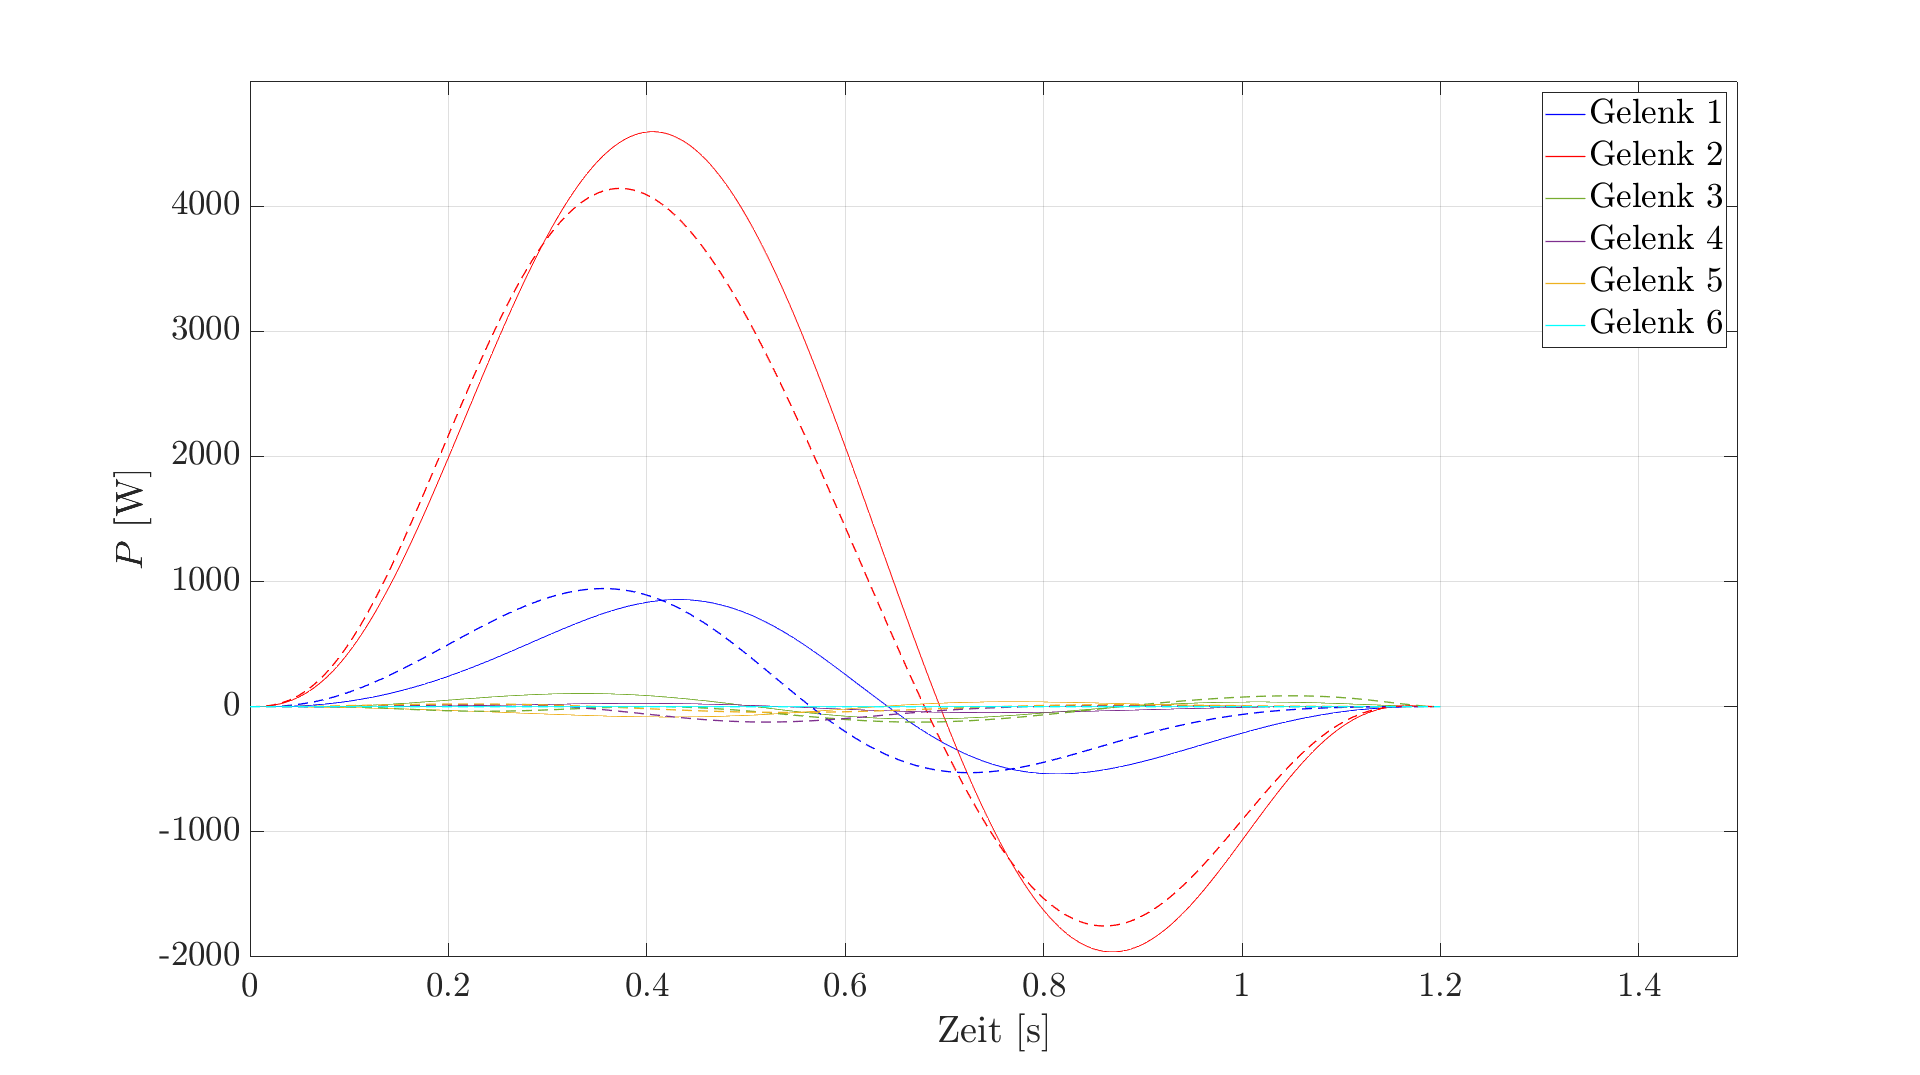
\includegraphics[width=1\linewidth]{images/Optimierungsergebnisse_up/popt}
	\caption{Simulierte Leistungsaufnahme der Initialbahn und optimierten Bewegungsbahn}
	\label{fig:popt}
\end{figure}
%
Nachfolgend werden die Geschwindigkeitsnebenbedingungen in Abbildung \ref{fig:velopt}sowie der Verlauf der Gelenkwinkel in Abbildung \ref{fig:posopt} untersucht. 
%
\begin{figure}[tbph]
	\centering
	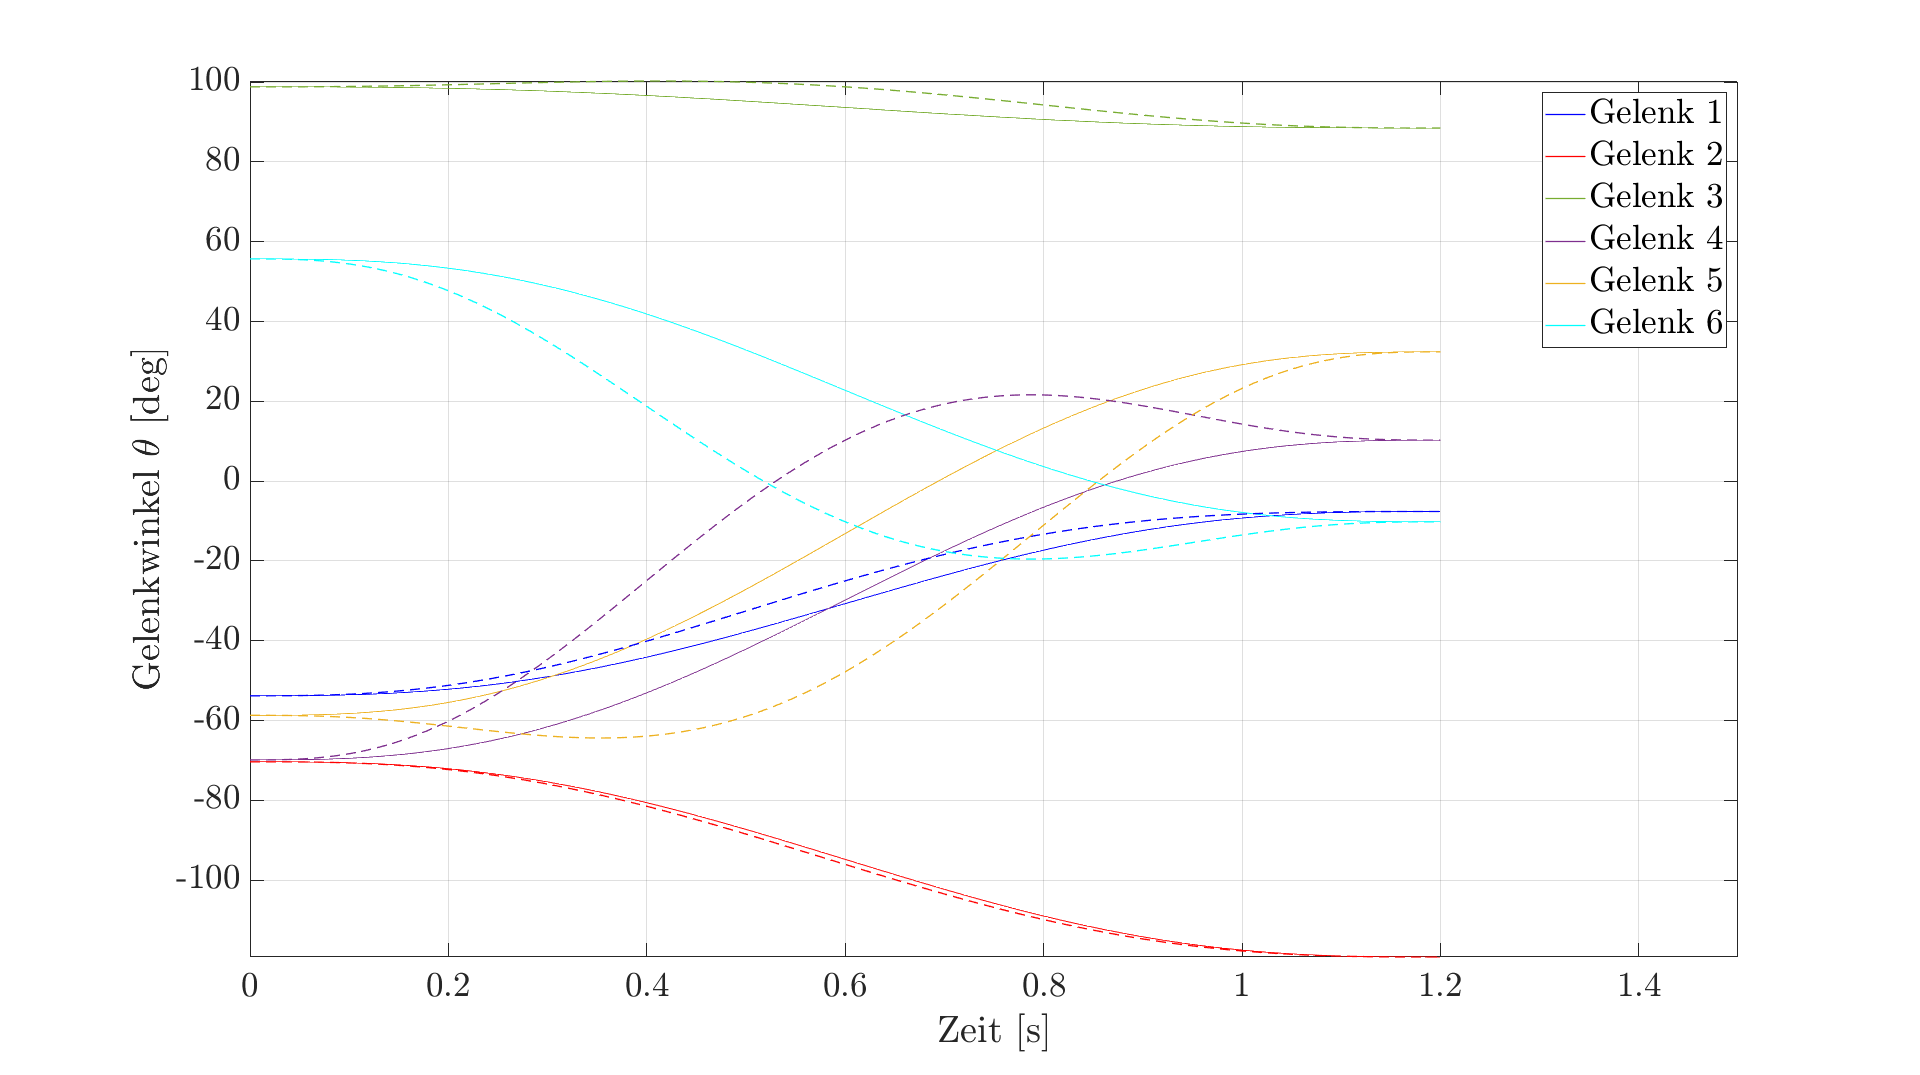
\includegraphics[width=1\linewidth]{images/Optimierungsergebnisse_up/posopt}
	\caption{Gelenkwinkelverläufe der Initialbahn und energieoptimierten Bewegungsbahn}
	\label{fig:posopt}
\end{figure}
%
\begin{figure}[tbph]
	\centering
	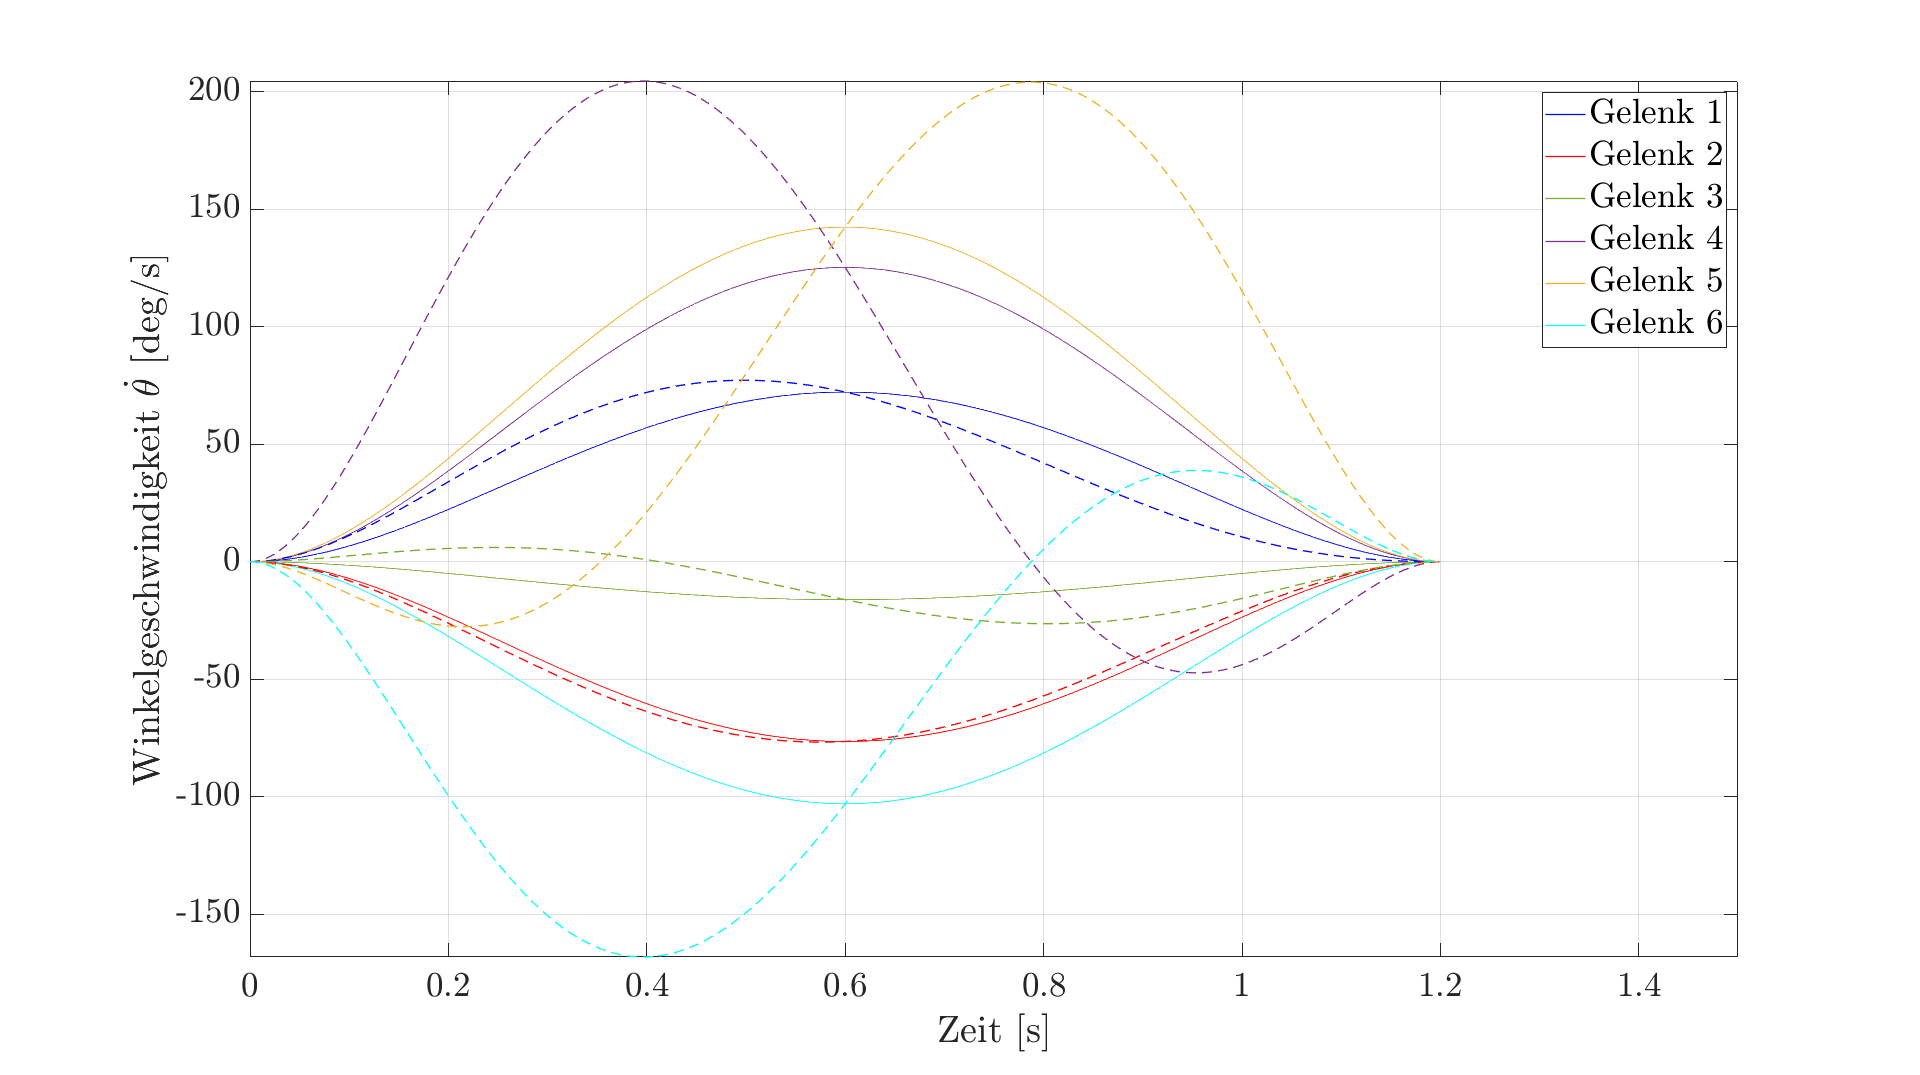
\includegraphics[width=1\linewidth]{images/Optimierungsergebnisse_up/velopt}
	\caption{Winkelgeschwindigkeitsverläufe der Initialbahn und energieoptimierten Bewegungsbahn}
	\label{fig:velopt}
\end{figure}
%
Für den Verlauf der Winkel im zweiten Gelenk sind keine auffälligen Abweichungen von der Initialbahn zu erkennen. Die beiden Verläufe der Gelenkwinkel eins und drei zeigen geringe Abweichungen im Bereich der Via-Punkte. Signifikante Unterschiede sind für die Verläufe der Gelenkwinkel vier, fünf und sechs erkennbar.  Bei Betrachtung der Abbildung \ref{fig:velopt} fällt auf, dass die Winkelgeschwindigkeiten $\dot{q}_{4}(t)$, $\dot{q}_{5}(t)$ und $\dot{q}_{6}(t)$ erheblich größer ausfallen als die Originalverläufe. Dies ist auf die Nähe der Gelenkwinkel ${q}_{v,4}$, ${q}_{v,5}$ und ${q}_{v,6}$ zu den Grenzwerten in Kombination mit der Größe des Gelenkwinkelhub $\Delta q_i = | q_{s,i}+q_{e,i} | ~\forall~ i \in \{4,5,6\}$ zurückzuführen. Infolgedessen werden die Via-Punkte ${q}_{v,4}$, ${q}_{v,5}$ und ${q}_{v,6}$ manuell auf den Mittelwert zwischen Initial-Via-Punkt und energieoptimalen Via-Punkt, siehe Gleichung \ref{eqn:manuellejustage} nachjustiert.
%
\begin{equation}
	\label{eqn:manuellejustage}
	{q}_{v,i,justiert} = \dfrac{{q}_{v,i,opt} + \dfrac{q_{s,i}+q_{e,i}}{2}}{2}~\forall~ i \in \{4,5,6\}
\end{equation}
%
Die resultierenden Winkelgeschwindigkeiten in Abbildung \ref{fig:veloptedit} und Winkelbeschleunigungen in Abbildung \ref{fig:accoptedit}  werden damit auf ein akzeptables Maß reduziert. Die energieoptimalen Verläufe sind gestrichelt, die justierten Verläufe gepunktet dargestellt.
%
\begin{figure}[tbph]
	\centering
	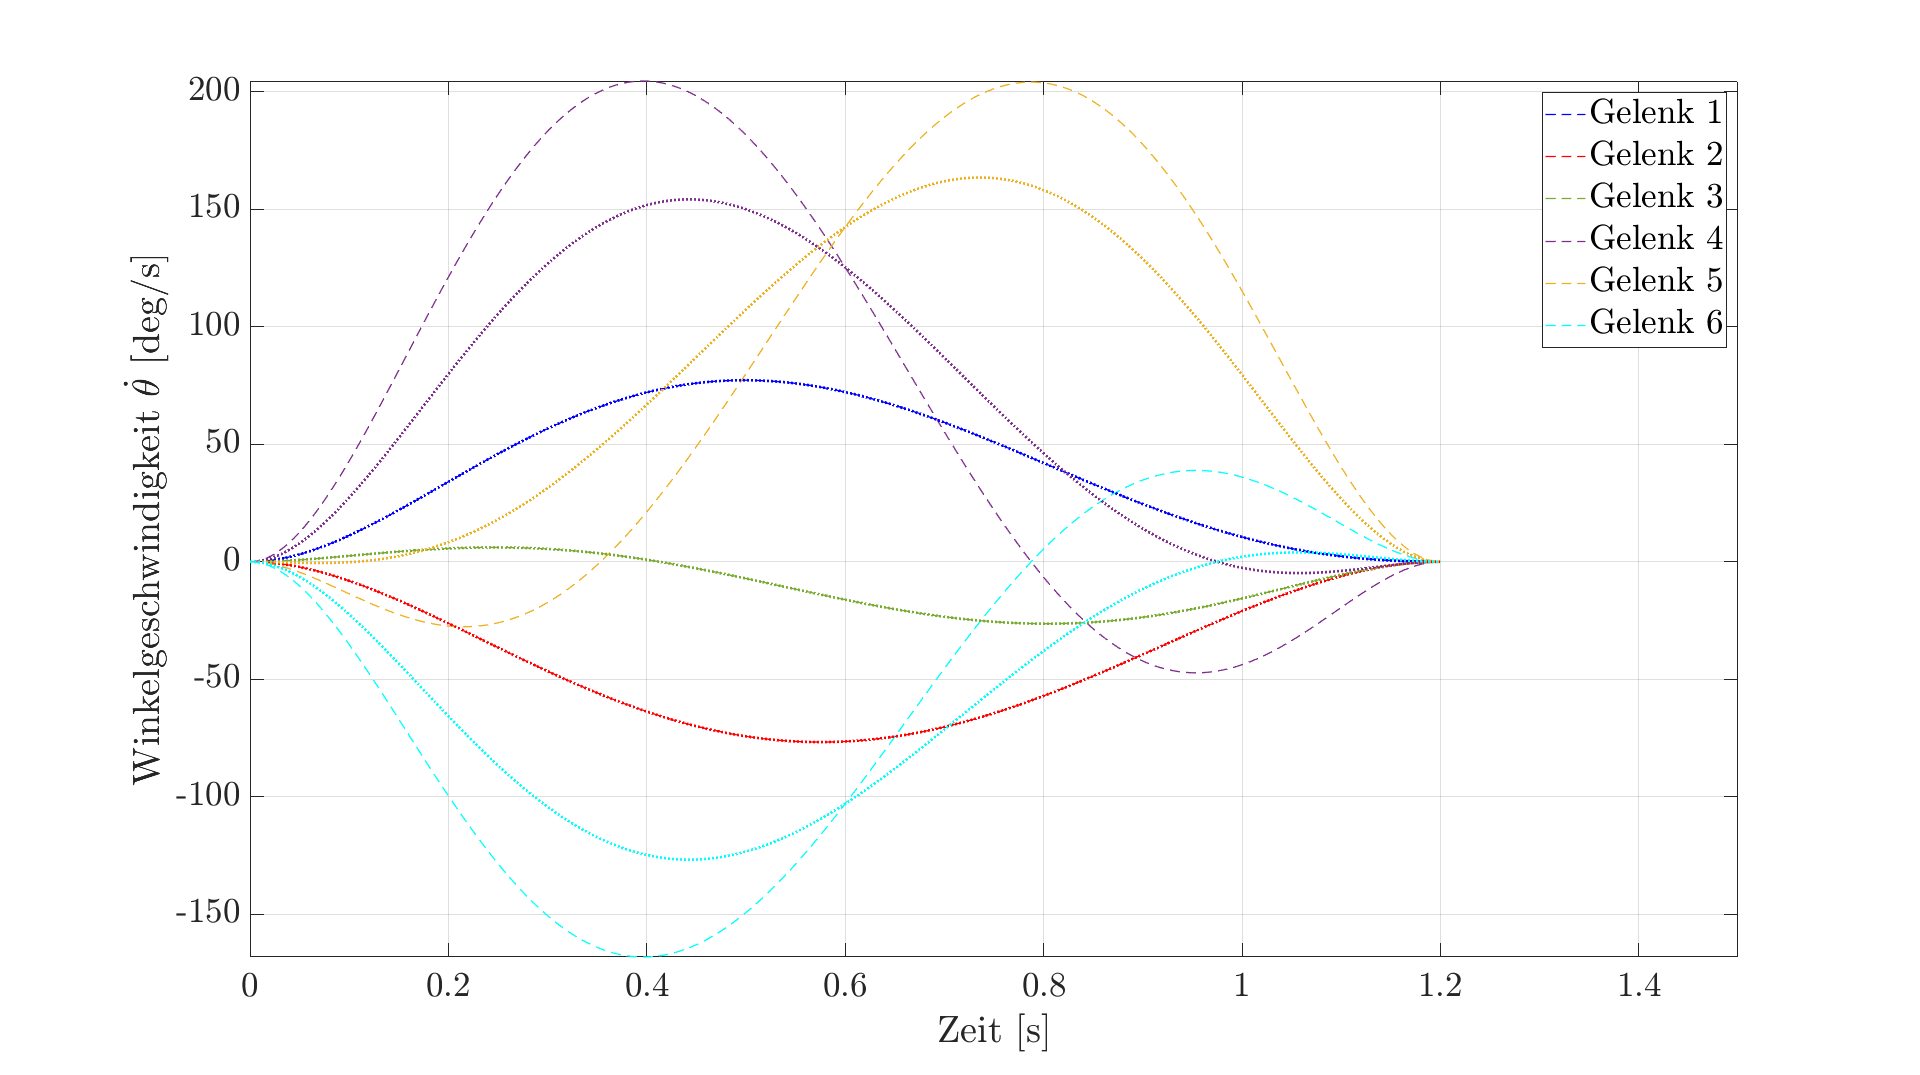
\includegraphics[width=1\linewidth]{images/Optimierungsergebnisse_up/veloptedit}
	\caption{Winkelgeschwindigkeitsverläufe der energieoptimierten Bewegungsbahn und justierten energieoptimierten Bewegungsbahn}
	\label{fig:veloptedit}
\end{figure}
%
\begin{figure}[tbph]
	\centering
	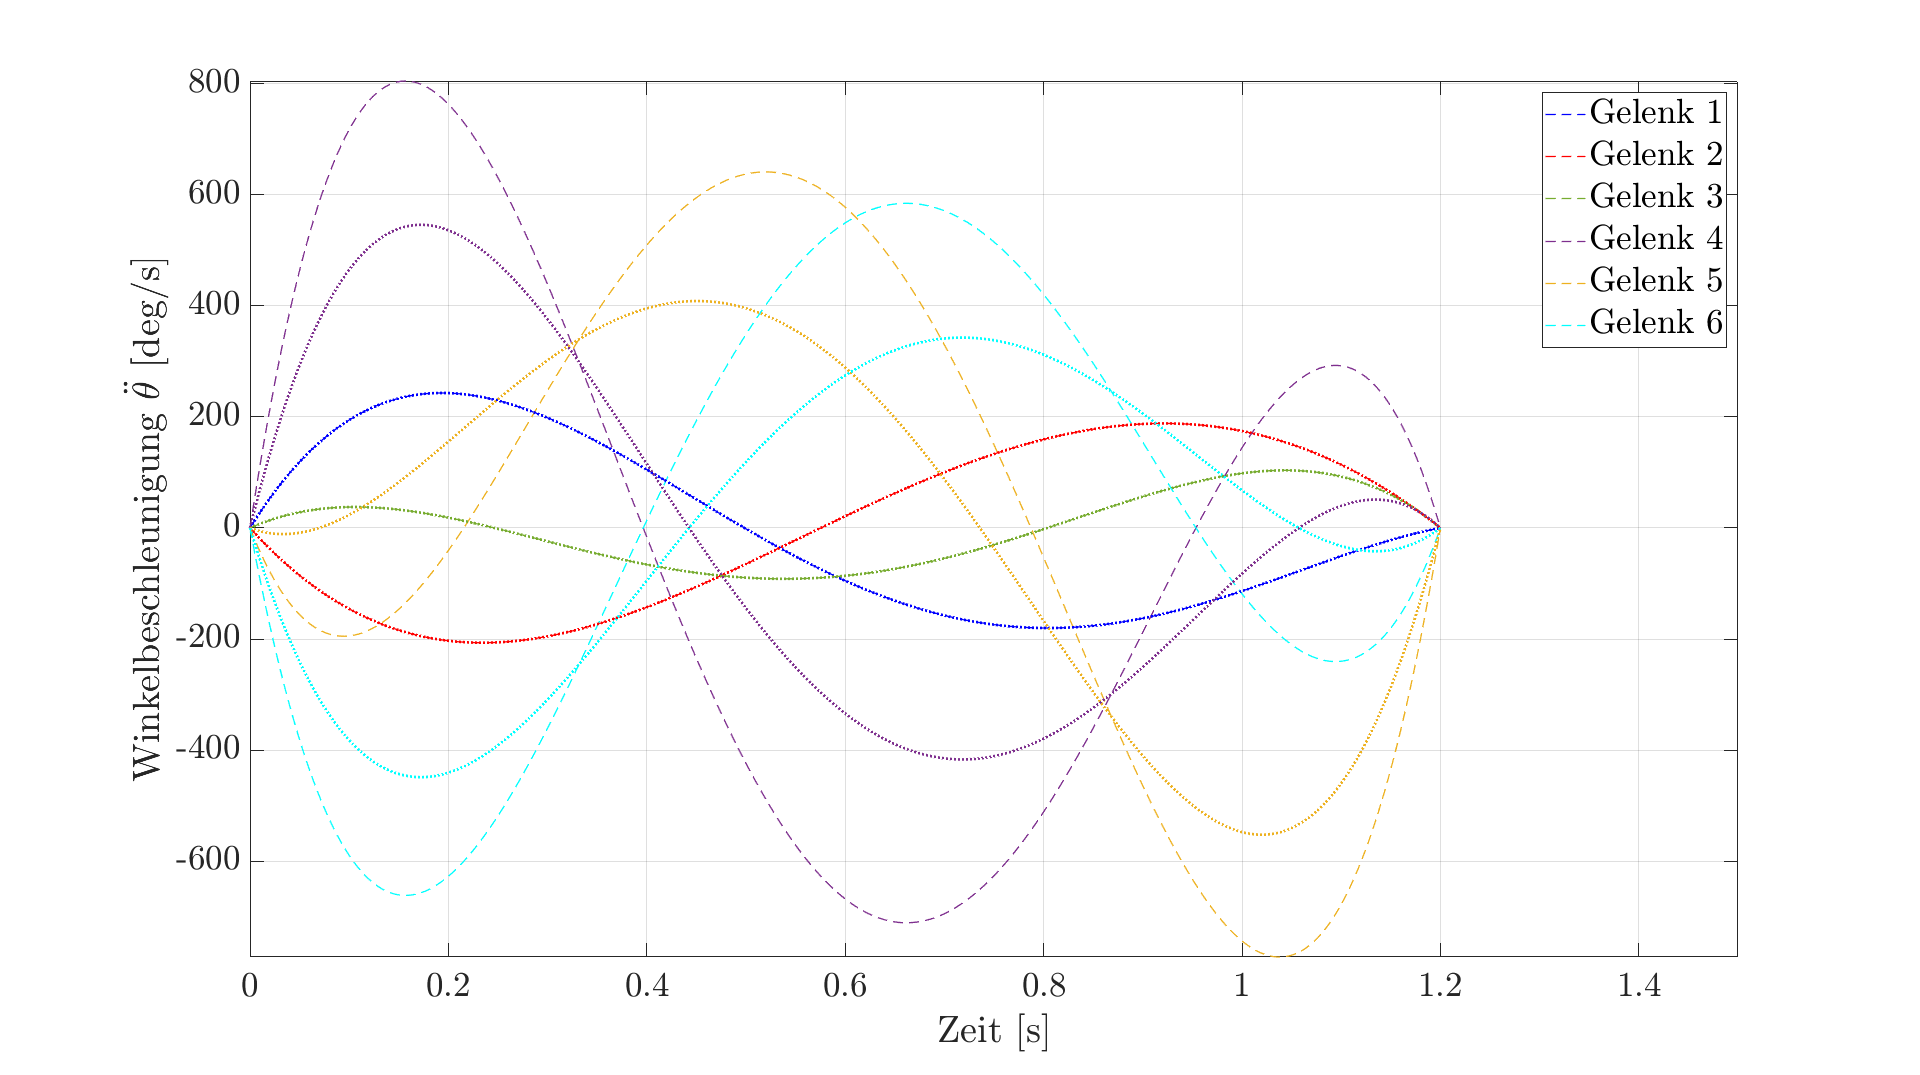
\includegraphics[width=1\linewidth]{images/Optimierungsergebnisse_up/accoptedit}
	\caption{Winkelbeschleunigungsverläufe der energieoptimierten Bewegungsbahn und justierten energieoptimierten Bewegungsbahn}
	\label{fig:accoptedit}
\end{figure}
%
Für den justierten Parametervektor beträgt der Energieverbrauch \textbf{1858 Joule} erzielt. Damit wird eine Energieeinsparung von 7,15 \% gegenüber der Initialbahn erzielt. Die Abbildungen für den Vergleich der initialen und justierten Verläufe aller relevanten Größen sind im Anhang \ref{acc:optupjust} aufgeführt.



\section{Validierung der Optimierungsergebnisse}
Ziel ist die Energieeinsparung auf Basis des optimierten Via-Punkts am realen System zu validieren. 
%
\subsection{Durchführung}
%Versuchsbeschreibung
%Definition von Start- und Zielpunkt
%Berechnung der Initialbahn durch die KR C
%Berechnung der Startviapunkte
\subsection{Auswertung}
%\begin{figure}[tbph]
%	\centering
%	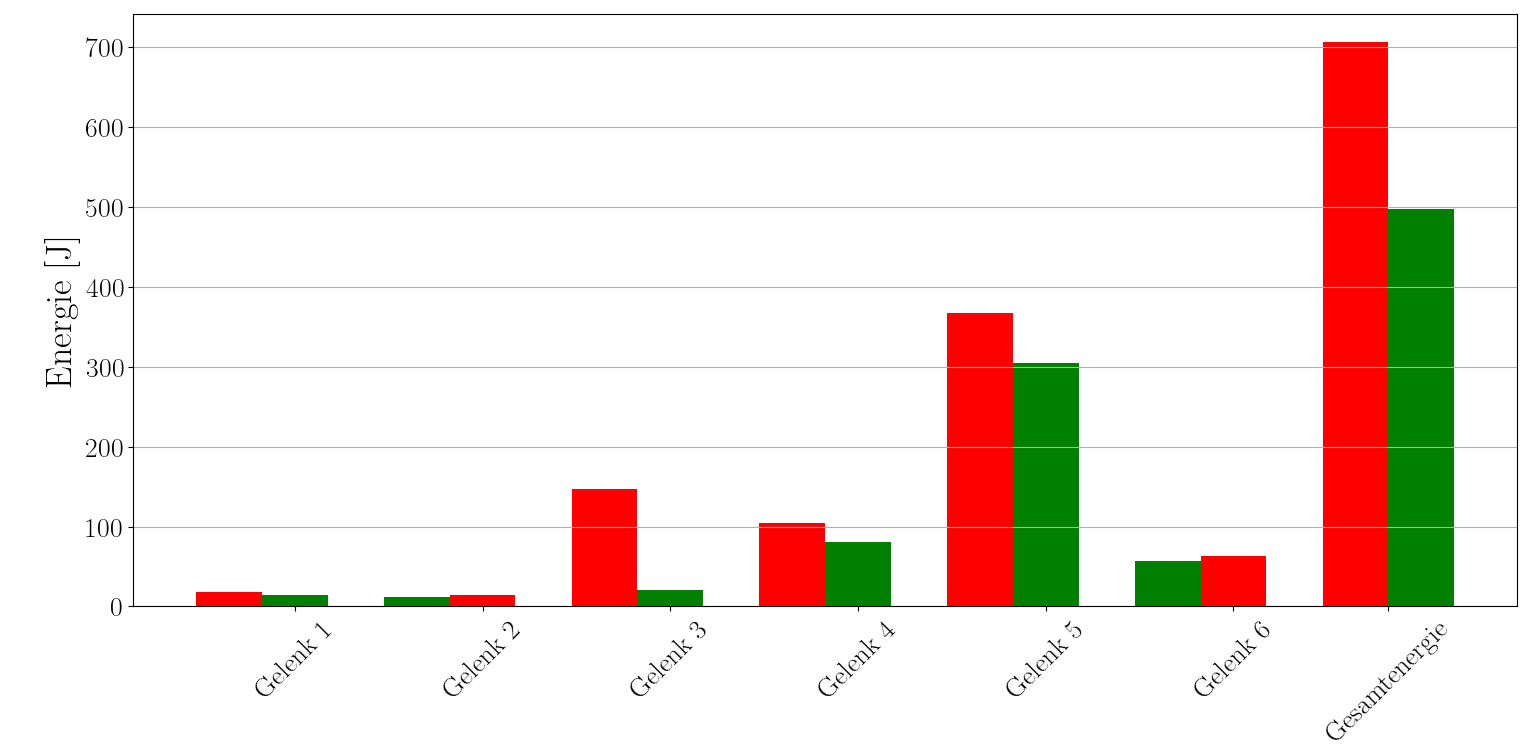
\includegraphics[width=1\linewidth]{images/e_down500}
%	\caption{Energieverbrauch Bewegung Eins}
%	\label{fig:edown500}
%\end{figure}
%\begin{figure}[tbph]
%	\centering
%	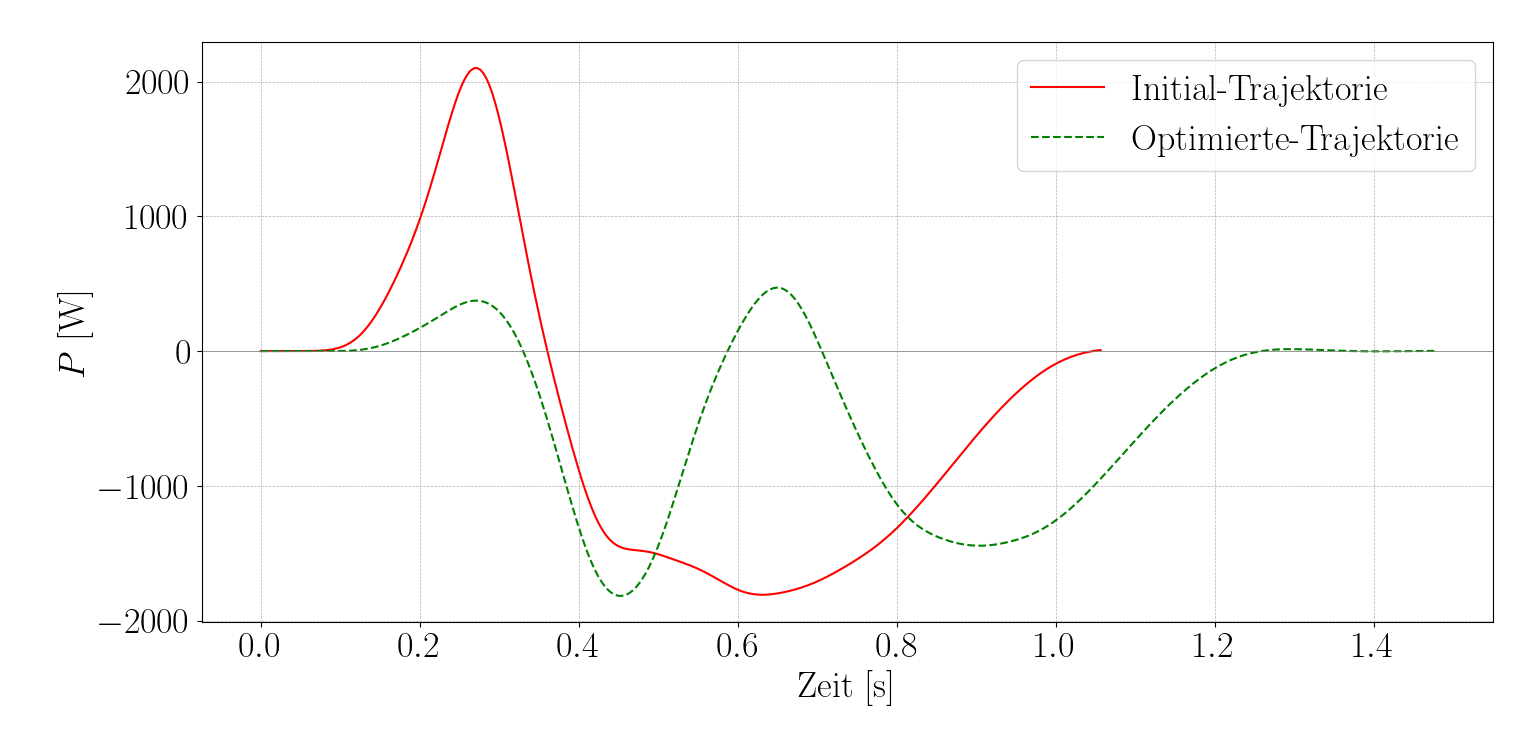
\includegraphics[width=1\linewidth]{images/P_down}
%	\caption{Leistungsaufnahme Bewegung Eins}
%	\label{fig:pdown}
%\end{figure}
%\begin{figure}[tbph]
%	\centering
%	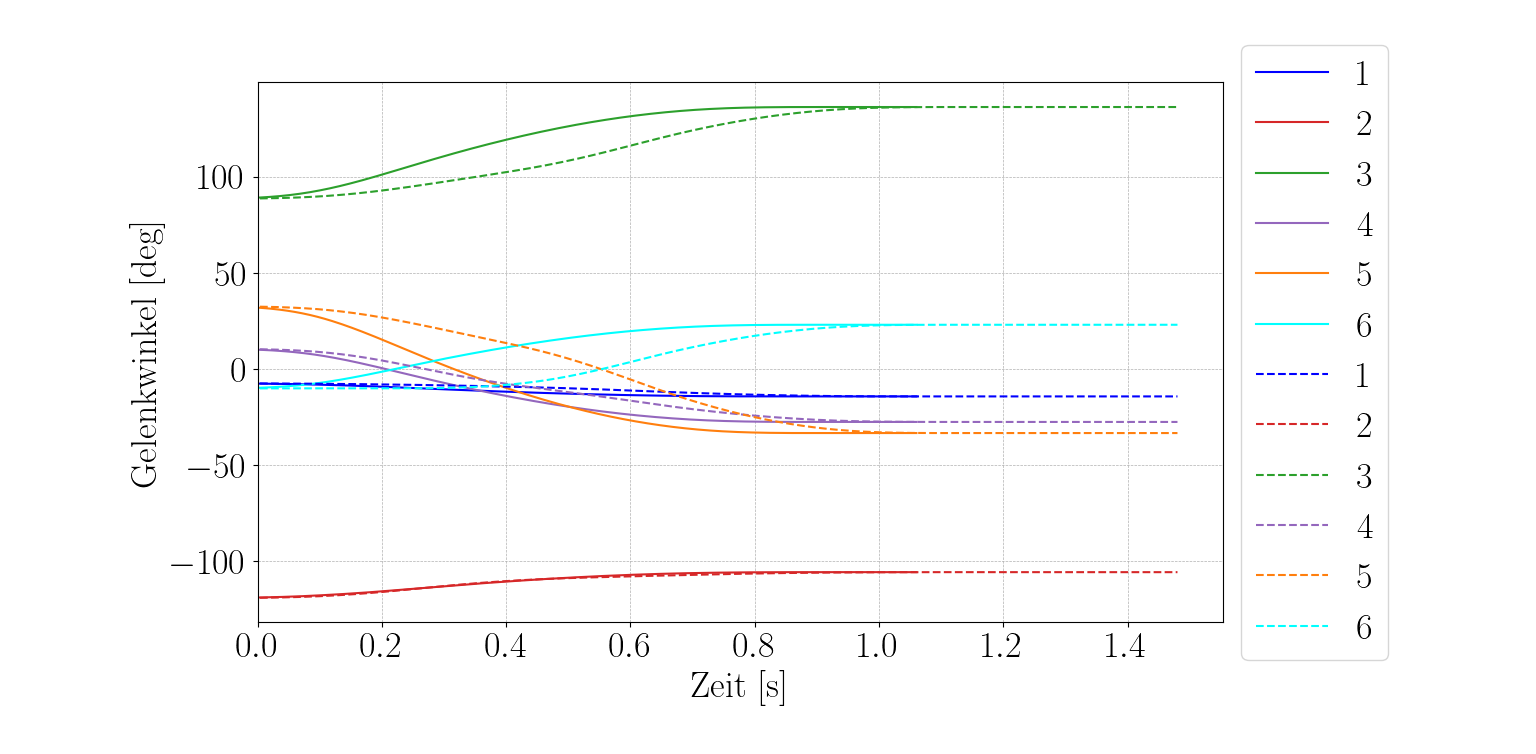
\includegraphics[width=1\linewidth]{images/aiposdown}
%	\caption{Gelenkwinkel Bewegung Eins}
%	\label{fig:aiposdown}
%\end{figure}
%\begin{figure}[tbph]
%	\centering
%	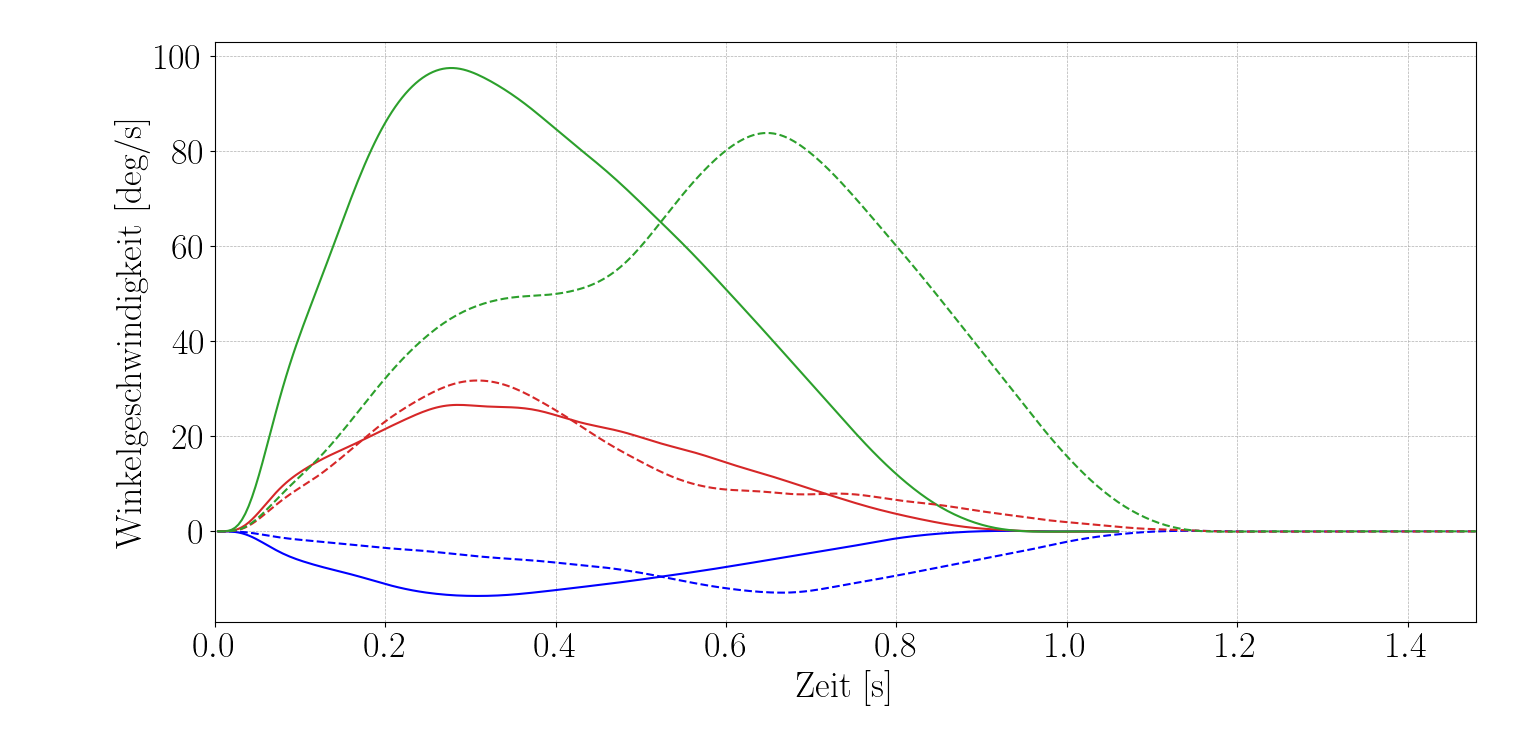
\includegraphics[width=1\linewidth]{images/velposdown1}
%	\caption{Winkelgeschwindigkeit in den Gelenken 1-3 Bewegung Eins}
%	\label{fig:velposdown1}
%\end{figure}
%\begin{figure}[tbph]
%	\centering
%	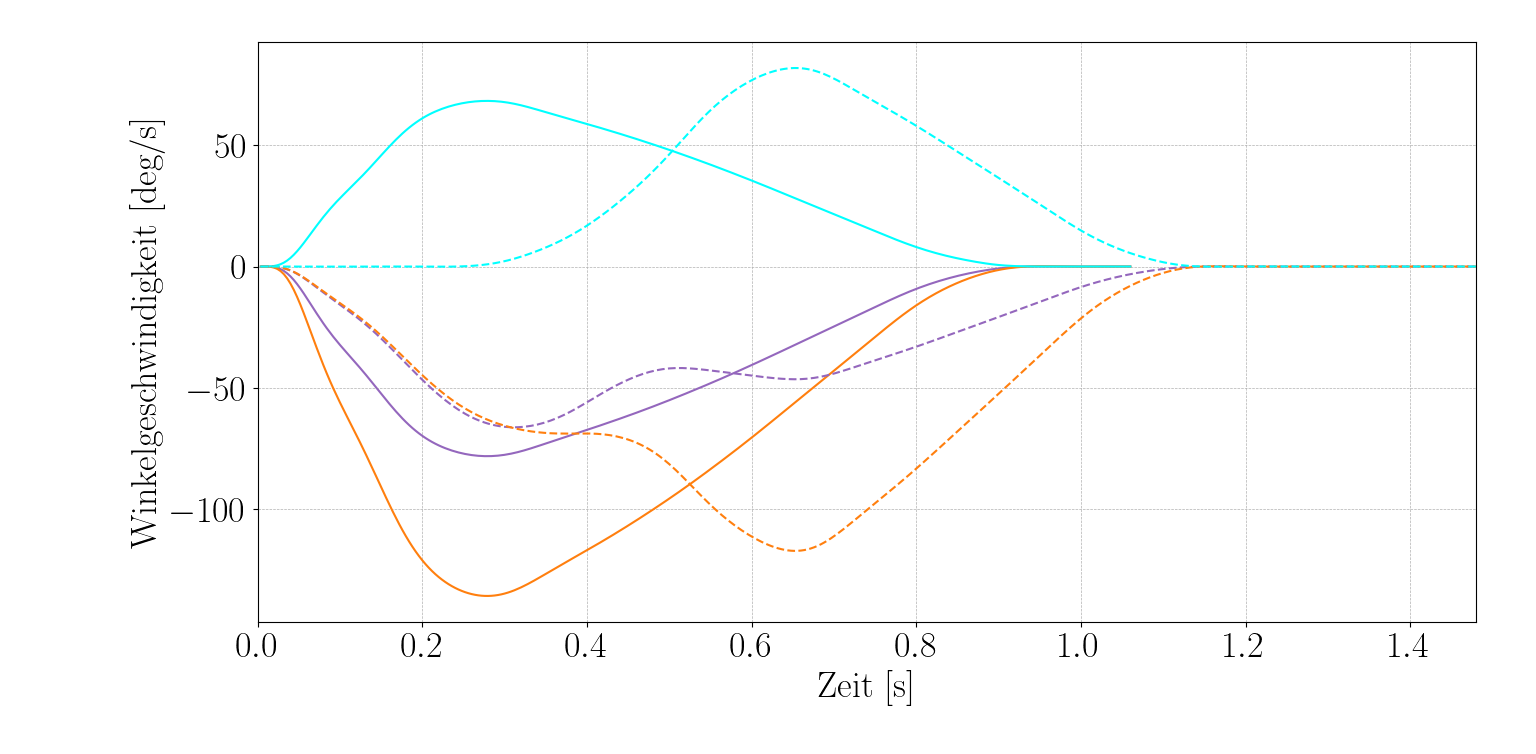
\includegraphics[width=1\linewidth]{images/velposdown2}
%	\caption{Winkelgeschwindigkeit in den Gelenken 4-6 Bewegung Eins}
%	\label{fig:velposdown2}
%\end{figure}
%\begin{figure}[tbph]
%	\centering
%	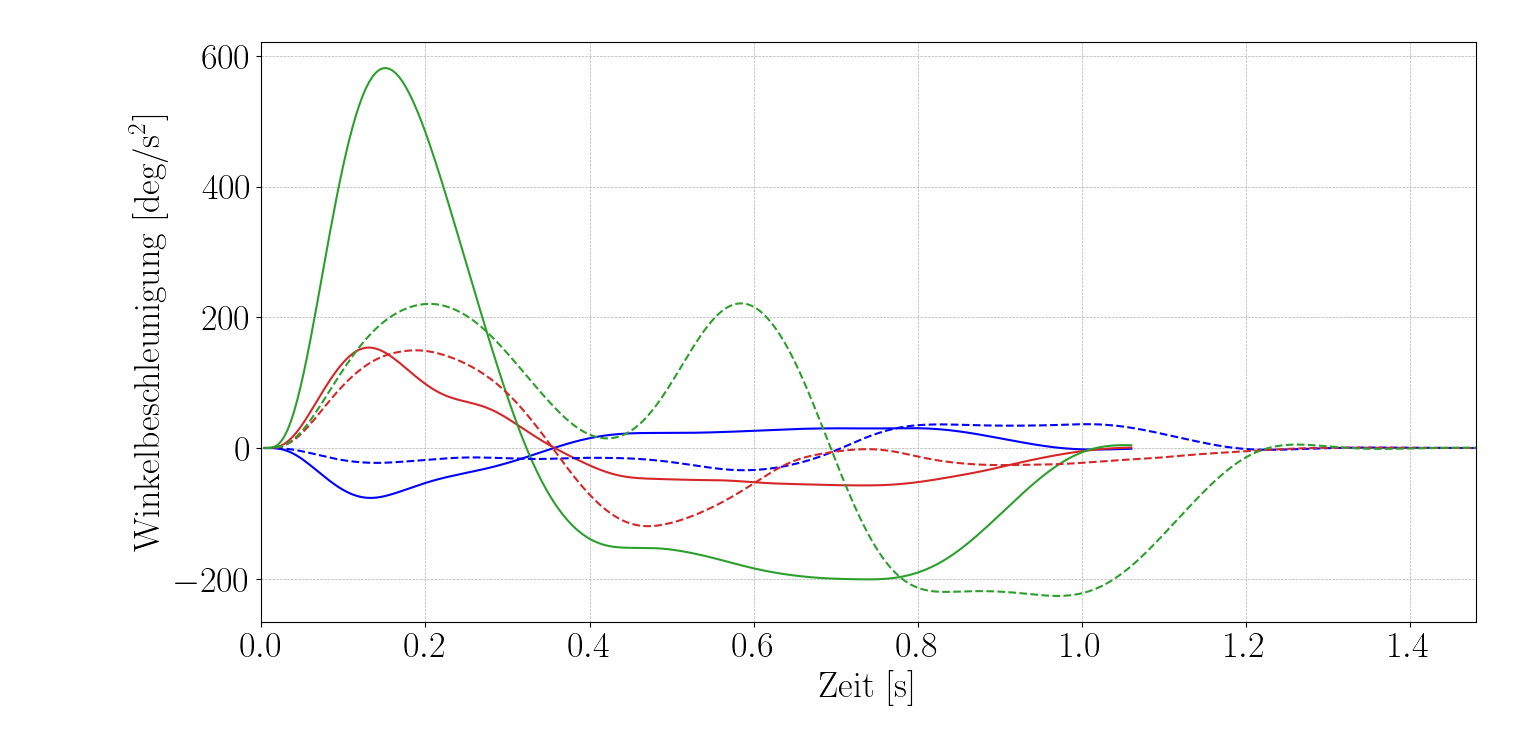
\includegraphics[width=1\linewidth]{images/accdown1}
%	\caption{Winkelbeschleunigung in den Gelenken 1-3 Bewegung Eins}
%	\label{fig:accdown1}
%\end{figure}
%\begin{figure}[tbph]
%	\centering
%	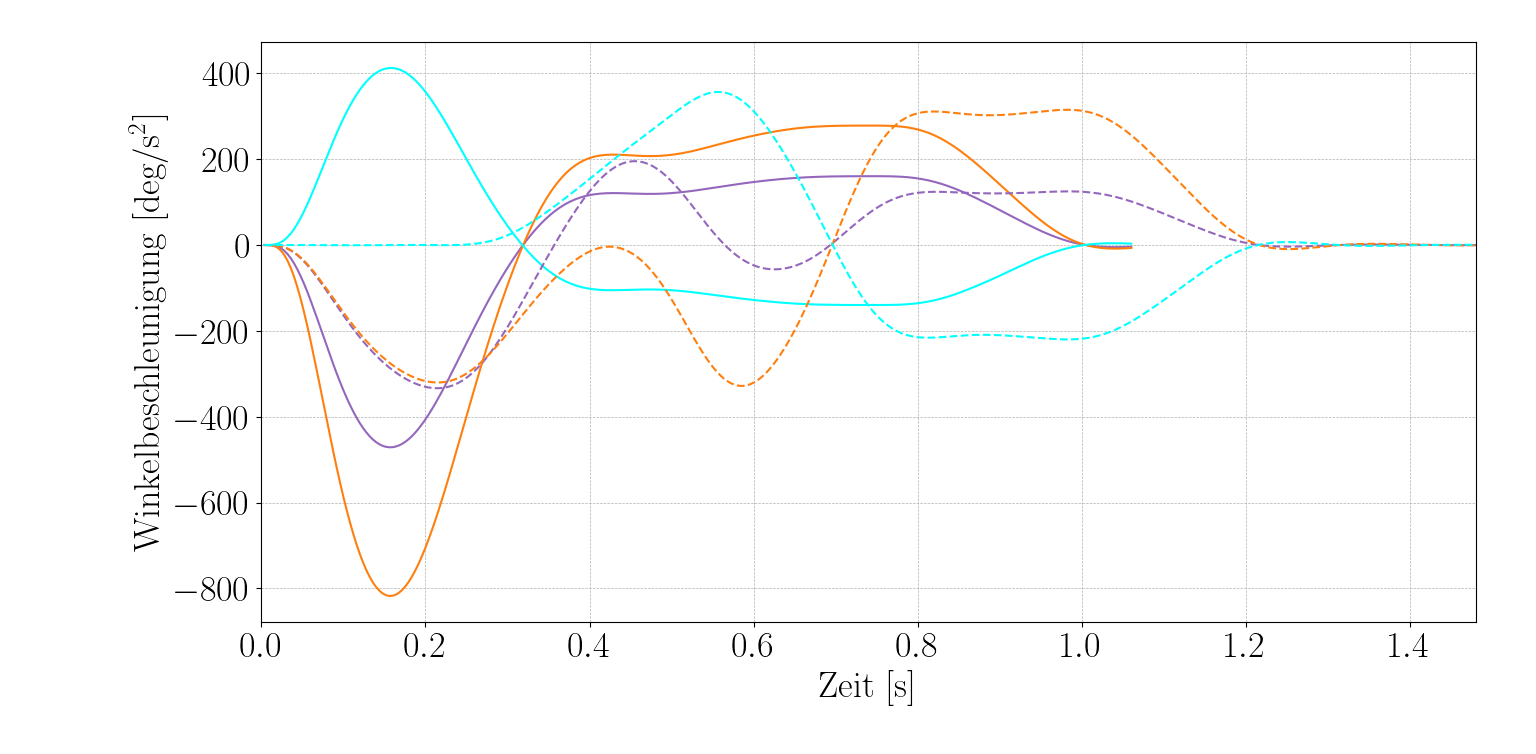
\includegraphics[width=1\linewidth]{images/accdown2}
%	\caption{Winkelbeschleunigung in den Gelenken 4-6 Bewegung Eins}
%	\label{fig:accdown2}
%\end{figure}
%
\begin{figure}[tbph]
	\centering
	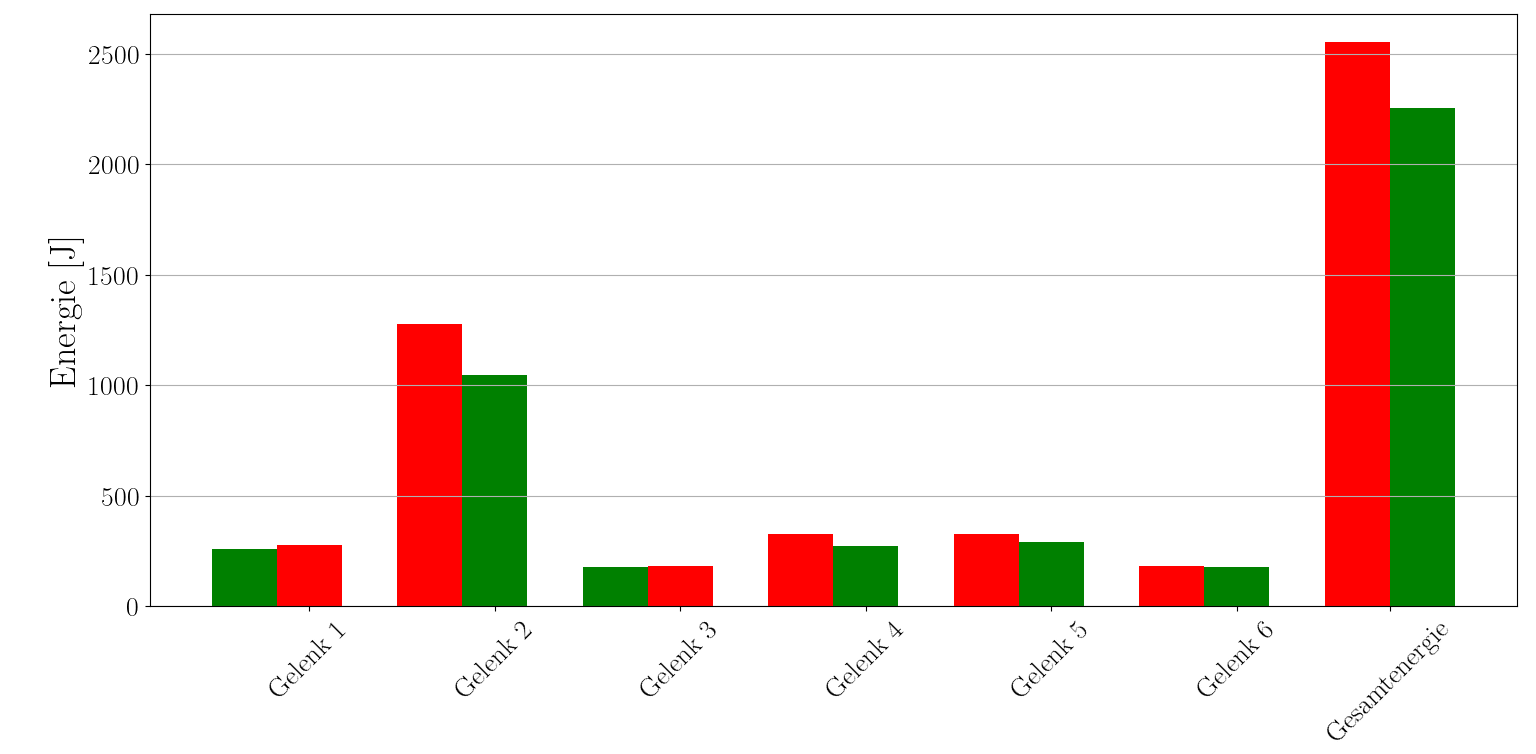
\includegraphics[width=1\linewidth]{images/e_up500}
	\caption{Energieverbrauch Bewegung Zwei}
	\label{fig:eup500}
\end{figure}
\begin{figure}[tbph]
	\centering
	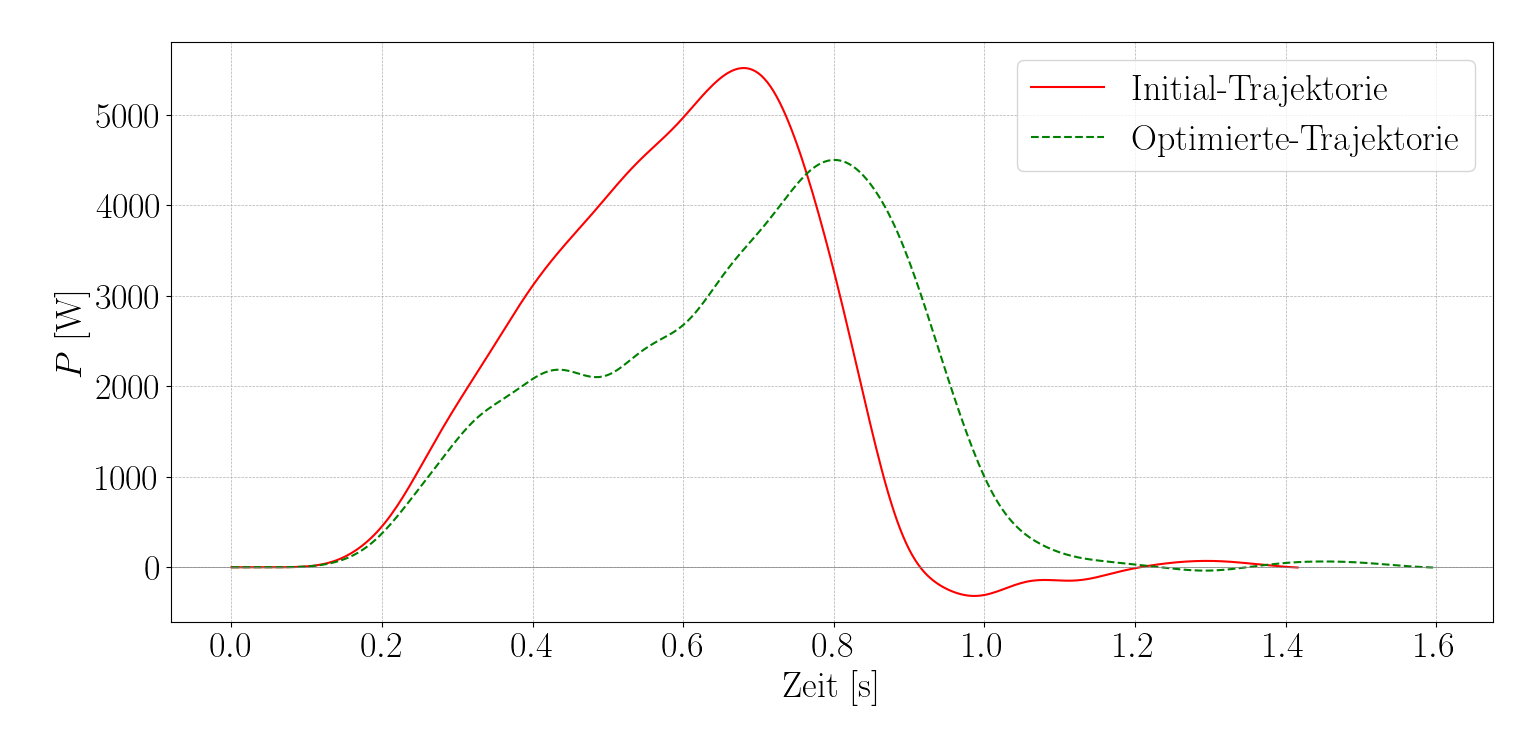
\includegraphics[width=1\linewidth]{images/P_up}
	\caption{Leistungsaufnahme Bewegung Zwei}
	\label{fig:pup}
\end{figure}
%\begin{figure}[tbph]
%	\centering
%	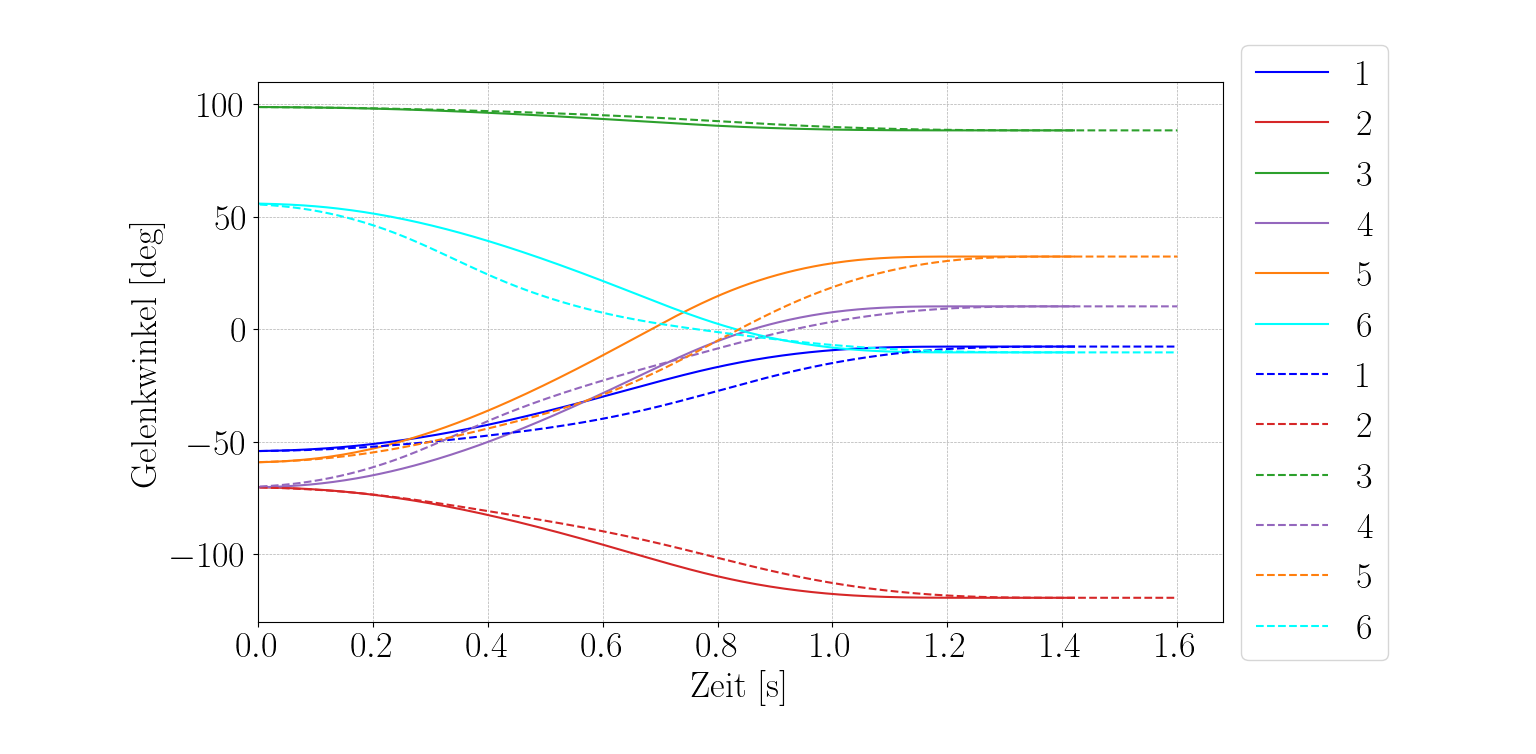
\includegraphics[width=1\linewidth]{images/aiposup}
%	\caption{Gelenkwinkel Bewegung Eins}
%	\label{fig:aiposup}
%\end{figure}
%\begin{figure}[tbph]
%	\centering
%	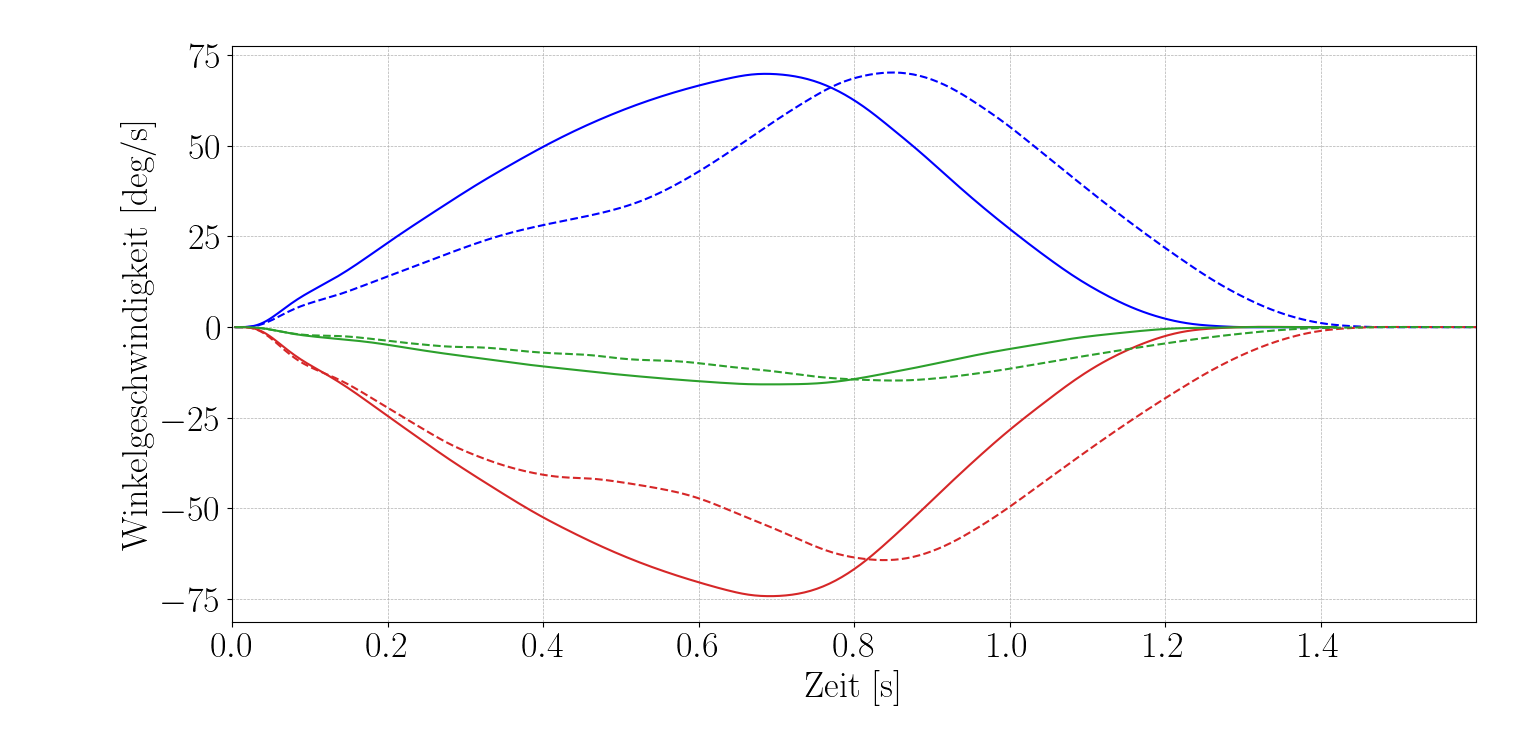
\includegraphics[width=1\linewidth]{images/velposup1}
%	\caption{Winkelgeschwindigkeit in den Gelenken 1-3 Bewegung Zwei}
%	\label{fig:velposup1}
%\end{figure}
%\begin{figure}[tbph]
%	\centering
%	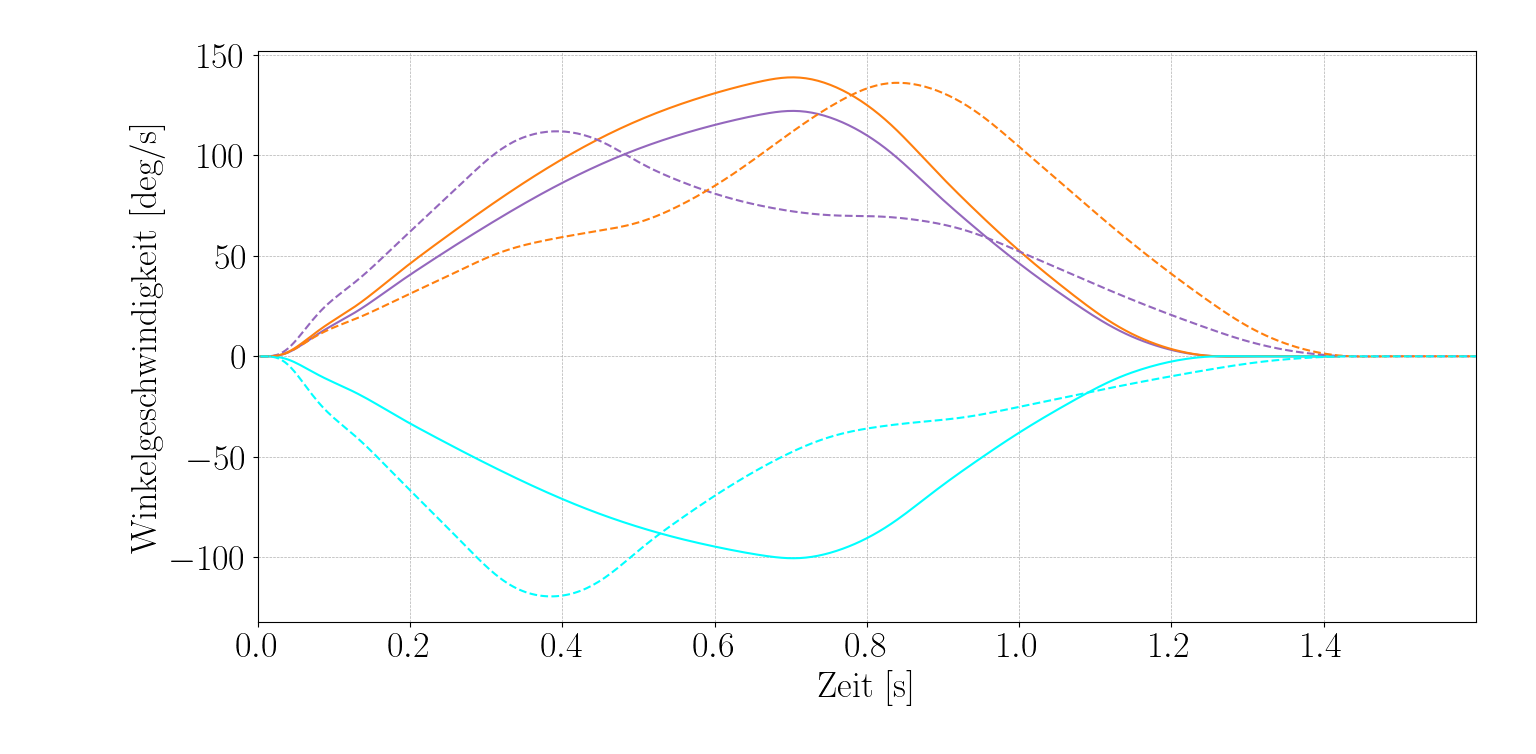
\includegraphics[width=1\linewidth]{images/velposup2}
%	\caption{Winkelgeschwindigkeit in den Gelenken 4-6 Bewegung Zwei}
%	\label{fig:velposup2}
%\end{figure}
%\begin{figure}[tbph]
%	\centering
%	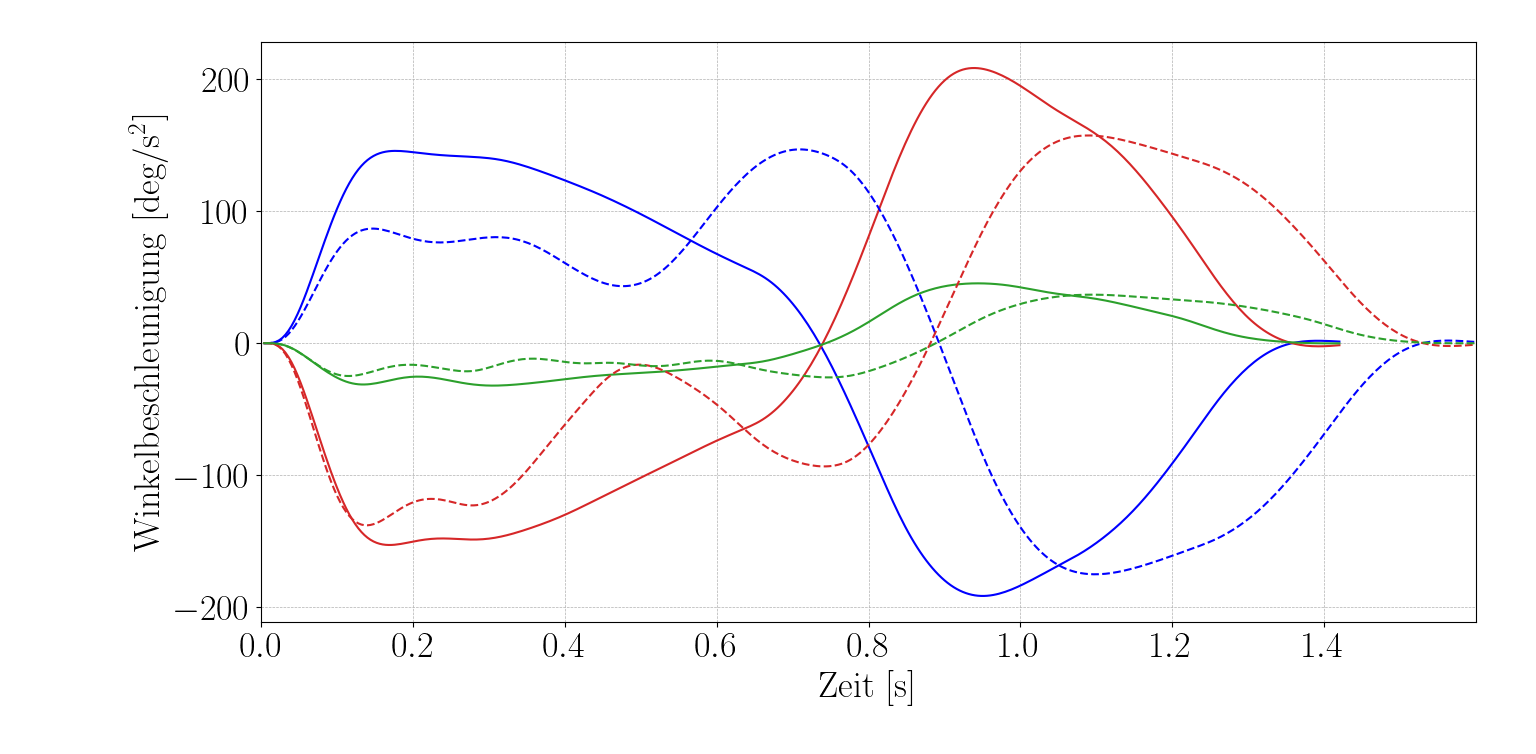
\includegraphics[width=1\linewidth]{images/accup1}
%	\caption{Winkelbeschleunigung in den Gelenken 1-3 Bewegung Zwei}
%	\label{fig:accup1}
%\end{figure}
%\begin{figure}[tbph]
%	\centering
%	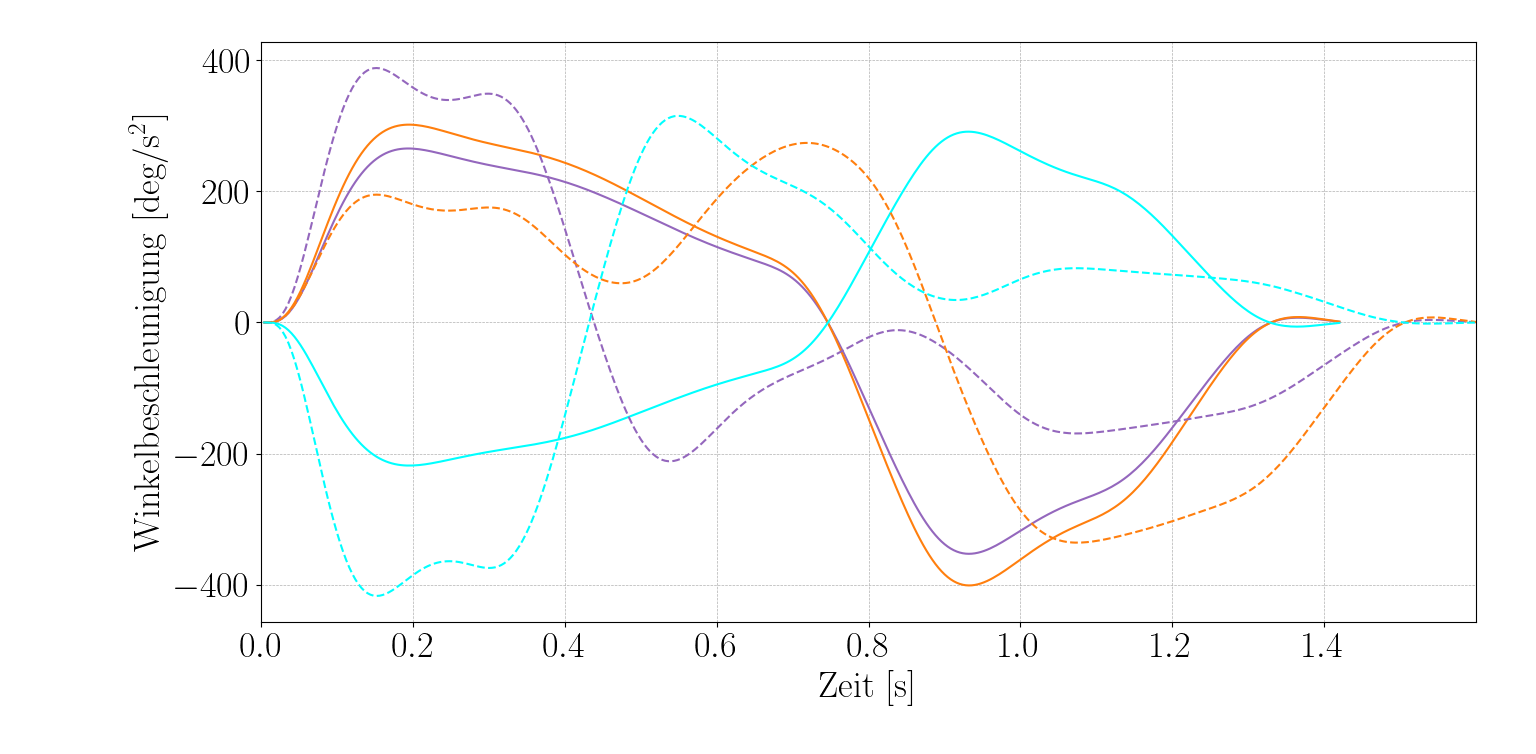
\includegraphics[width=1\linewidth]{images/accup2}
%	\caption{Winkelbeschleunigung in den Gelenken 4-6 Bewegung Zwei}
%	\label{fig:accup2}
%\end{figure}

\subsection{Schlussfolgerung} 

%

%\subsection{Fehlerquellen}
%Temperatureinfluss auf die Reibung 
\chapter{Validierung der Optimierungsergebnisse}
\label{cha:Validierung}
%... Verifikation, Auswertung, Lösungsbewertung, Diskussion der Ergebnisse
%Anwendung auf bestehende Systeme, ohne dass die Hardware 
%negative  Ergebnisse 
%lokales minimum 
Das Ziel der Validierung besteht darin, die in der Simulation berechneten Energieeinsparungen am realen System mithilfe des optimierten Parametervektors nachzuweisen. Der Optimierer wurde gegenwärtig nur an einem einzigen Pfad für den Roboter getestet. Von einer Abbildung der Validierung auf weitere Optimierungsversuche wird abgesehen. Diese sind im Einzelfall zu überprüfen. Der Messaufbau ist identisch zu der Beschreibung im Kapitel \ref{sec:modellvalidierung} Validierung des Roboterdynamik-Modells. 
%
\section{Durchführung}
Roboterprogramme werden auf der KR C5 in der Programmiersprache KUKA Robot Language-(KRL) geschrieben. Ein KRL-Programm ist dabei aus einer Source-Datei (src) und einem data-file (dat)  aufgebaut. Der justierte-energieoptimierte Parametervektor $\bm{q}_v$ wird auf der KR C5 zwischen dem Start- und Zielpunkt der letzten Bewegungsbahn des Programms $Kleben-Seitenwand$ als Via-Punkt \lstinline|ViaJustOptUp| in der src-Datei angelegt. 
\begin{lstlisting}[numbers=none]
	;FOLD PTP ViaJustOptUp Vel=100 % PDAT8 Tool[1] Base[0] ;%{PE}
\end{lstlisting}
Ohne einen expliziten Überschleifbefehl fährt der Roboter den Via-Punkt millimetergenau an und reduziert seine Geschwindigkeit bei Erreichen des Punkts auf Null. In der Problemstellung der Arbeit wurde eine signifikante Abweichung von der originalen Bewegungsdauer als unzulässig definiert. 
Infolgedessen wird der Implementierte Via-Punkt in der src-Datei um den KRL Überschleifbefehl \lstinline|CONT| erweitert. 
%
\begin{lstlisting}[numbers=none]
	;FOLD PTP ViaJustOptUp CONT Vel=100 % PDAT8 Tool[1] Base[0] ;%{PE}
\end{lstlisting}
%
Zusätzlich muss der Robotersteuerung mitgeteilt werden, in welchem Modus der Via-Punkt zu überschleifen ist und welcher Überschleifradius angewendet werden soll. Dies erfolgt in der im dat-file über die Parameterdefinition \lstinline|PDAT|, welchen dem Via-Punkt in der src-datei zugewiesen ist. 
Die Approximationsmethode \lstinline|APO_MODE| wird mit \lstinline|CDIS| festgelegt. D. h. ein Überschleifen beginnt frühestens, wenn die Entfernung zum Punkt den Wert von \lstinline|APO_DIST = 500 mm| unterschreitet \cite[S.~578]{KSS.2023}.
\begin{lstlisting}[numbers=none]
	DECL PDAT PPDAT8={VEL 100.0000,ACC 100.000,APO_DIST 500.000,APO_MODE #CDIS,GEAR_JERK 100.000,EXAX_IGN 0}
\end{lstlisting}
Die maximale Überschleifdistanz wird auf 500 mm festgelegt. Von der Nutzung des maximal möglichen Überschleifradius 1000 mm wird Abstand genommen, um das Risiko einer Kollision des Roboters mit peripheren Bauteilen zu begrenzen. Die neu programmierte Bewegung wird zunächst auf Kollisionsfreiheit durch manuelles Abfahren mit reduzierter Geschwindigkeit in der KUKA Betriebsart T1 getestet. Nach einer Verifizierung der Überschleif-Bewegung für eine programmierte Geschwindigkeit von 50\% in der Betriebsart T2 erfolgt die Signalaufzeichnung der justierten-energieoptimierten Trajektorie mit einer programmierten Geschwindigkeit von 100\%. 
%
\section{Auswertung}
Die über alle sechs Gelenke summierte Leistungsaufnahme des Roboters wird in \ref{fig:pup} abgebildet. 
%
\begin{figure}[tbph]
	\centering
	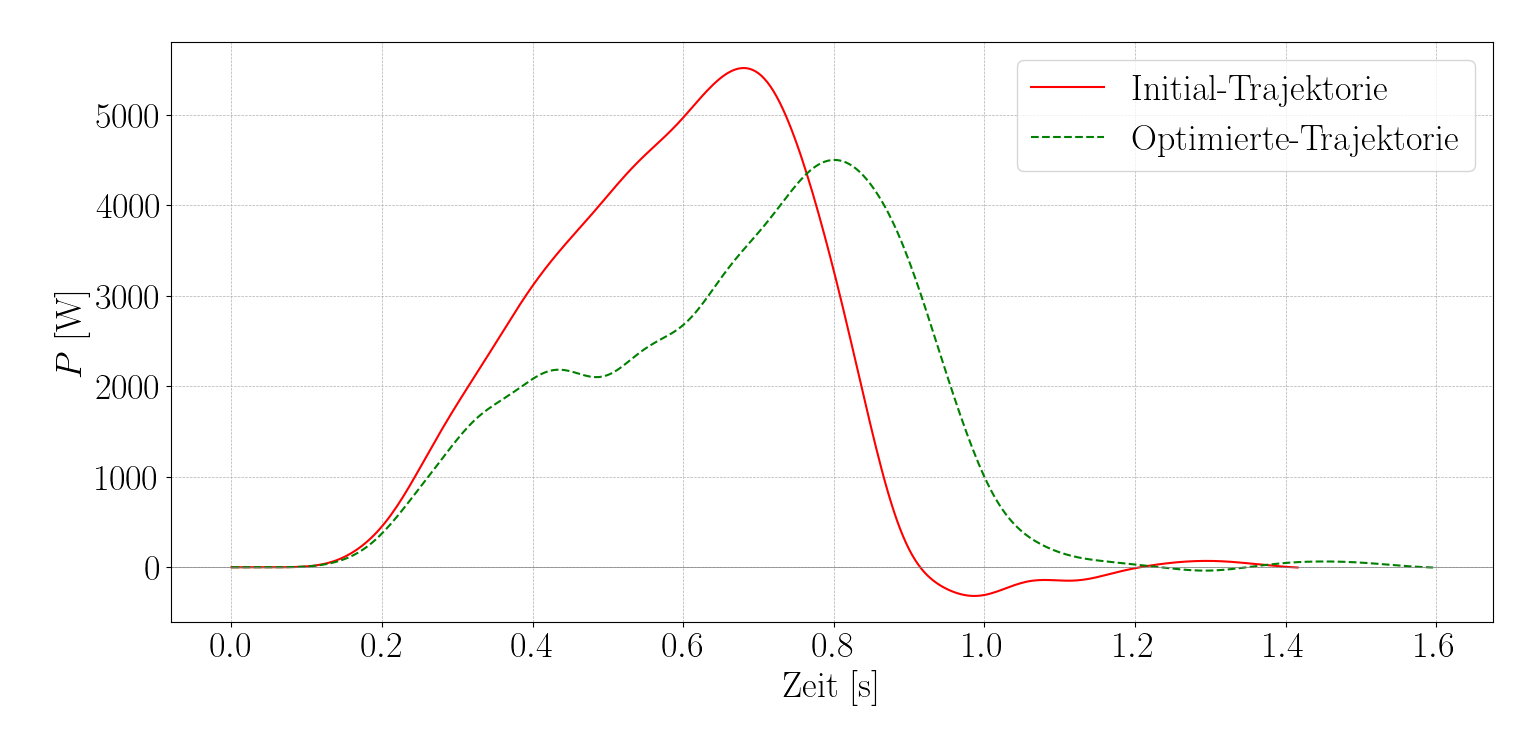
\includegraphics[width=1\linewidth]{images/P_up}
	\caption{Summierte Leistungsaufnahme des Roboters für den Verfahrweg vom letzten Prozesspunkt auf die  Home Position im Programm $Kleben-Seitenwand$}
	\label{fig:pup}
\end{figure}
%
Dabei ist eine Zunahme der Bewegungsdauer für die justierte-energieoptimierte Trajektorie um ca. 0,2 s gegenüber der Initial-Trajektorie festzustellen. Die exakte Dauer kann nur näherungsweise angegeben werden. Dies liegt an der im Rahmen der Arbeit entwickelten Datenverarbeitung. Die über den RSI aufgezeichneten und am Server empfangenen Signale werden nachträglich separiert und der einzelnen Bewegungen zugewiesen. Eine neue Bewegung wird beim Durchlaufen einer niedrig gewählten Leistungsschwelle indiziert. Die leichte Zunahme der Bewegungsdauer wird  dem zusätzlichen Programmschritt durch die Definition des Via-Punkts mit \lstinline|CDIS=500 mm| angerechnet. In der PTP-Bewegungsart führt der Roboter den TCP entlang der schnellsten Bahn zum Zielpunkt \cite[S.~429]{KSS.2023}. Der Via-Punkt hat zur Folge, dass der TCP nicht mehr auf der schnellsten Bahn geführt wird. Die maximal aufgenommene Momentanleistung konnte um ca. 1 kW gesenkt werden. 
Gegenüber der stetig ansteigenden Leistungsaufnahme der Initial-Trajektorie weißt die Leistungskurve der Optimierten-Trajektorie einen Sattel auf.  Der Verlauf der simulierten Leistung, siehe Abbildung \ref{fig:poptfinal}, sowie die im Anhang hinterlegten, simulierten Bewegungsdaten weisen dagegen keine Unstetigkeit auf. Die dem Sattel zugrunde liegende temporäre Reduktion der Geschwindigkeit setzt auf der Hälfte der Bewegungsdauer zwischen dem Start und dem Via-Punkt ein. Die Ursache dafür liegt in der Begrenzung der Geschwindigkeit des sechsten Gelenks. In der Konsequenz ist der Optimierer um die Geschwindigkeitsnebenbedienung \ref{eqn:conacc}, sowie die im Kapitel \ref{sec:Nebenbedingungen} genannten und in \cite[S.~5]{Hansen.2012} beschriebenen Formulierungen zur Begrenzung der maximalen Beschleunigung bzw. des maximalen Drehmoments zu erweitern. 
%\begin{figure}[tbph]
%	\centering
%	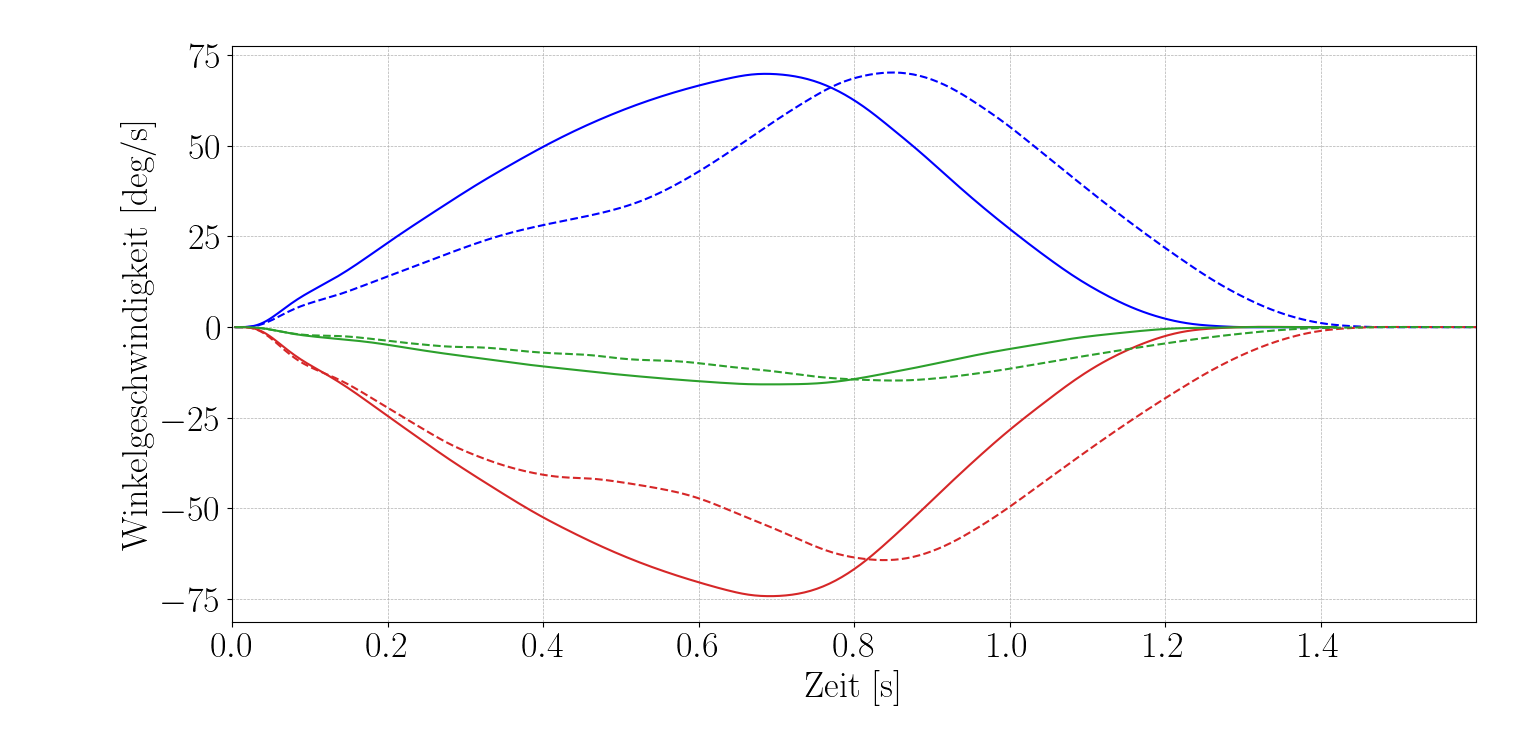
\includegraphics[width=1\linewidth]{images/velposup1}
%	\caption{Winkelgeschwindigkeit in den Gelenken 1-3 Bewegung Zwei}
%	\label{fig:velposup1}
%\end{figure}
Die über den optimierten Via-Punkt erzielte Energieeinsparung wird in der Grafik \ref{fig:eup500} dargestellt. Die Prognose der Simulation, dass die höchste Einsparung für das zweite Gelenk zu verzeichnen ist, wird erfüllt. Wie erwartet ist für den mechanischen Energieverbrauch im ersten Gelenk eine leichte Zunahme festzustellen. Die Optimierungsergebnisse werden in der Konsequenz als plausibel eingestuft. 
%
\begin{figure}[tbph]
	\centering
	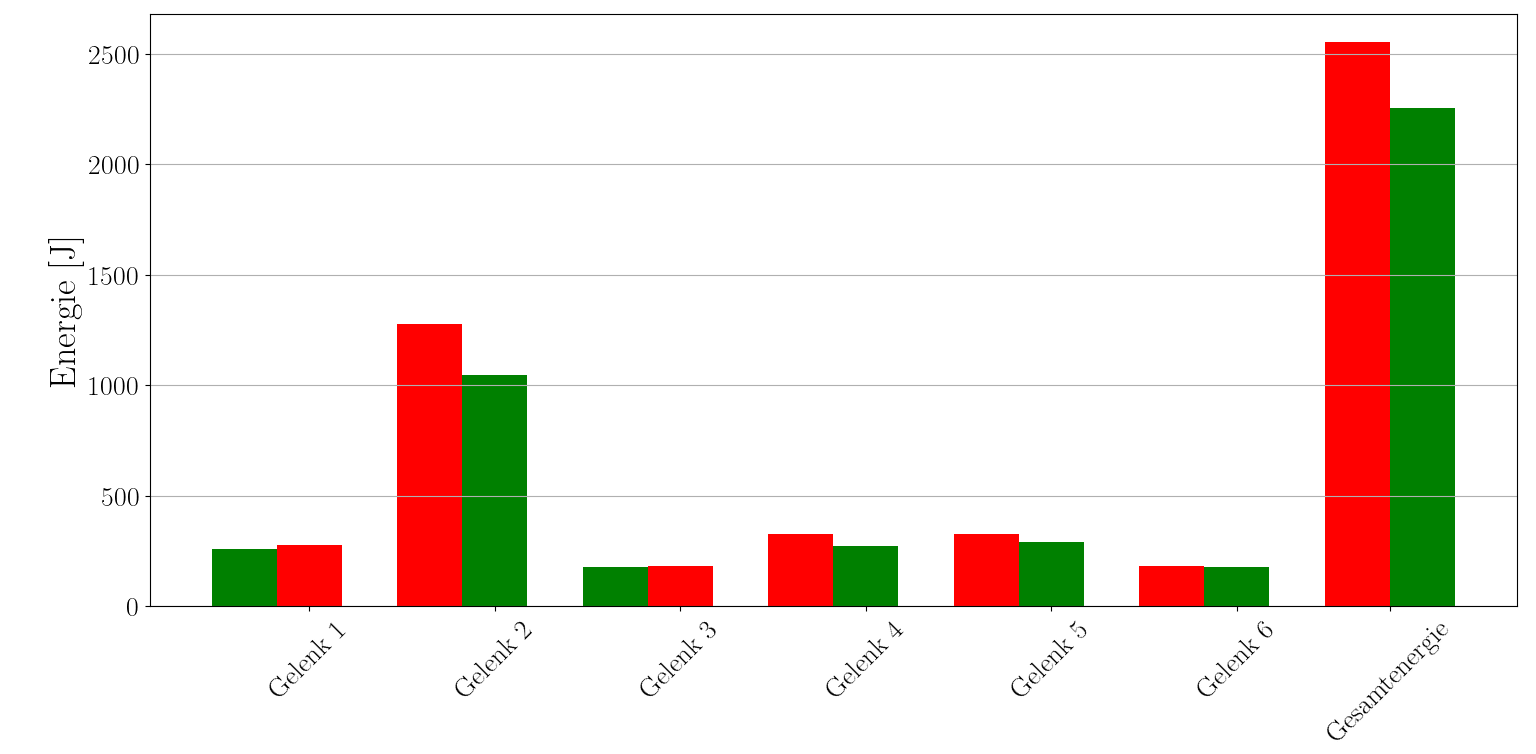
\includegraphics[width=1\linewidth]{images/e_up500}
	\caption{Energieverbrauch des Roboters für den Verfahrweg vom letzten Prozesspunkt auf die  Home Position im Programm $Kleben-Seitenwand$}
	\label{fig:eup500}        
\end{figure}
%
\chapter{Bewertung der Optimierungsergebnisse}
\label{cha:Bewertung}
Der Arbeit liegt die Forschungsfrage zugrunde, ob ein für die Produktion entwickeltes Roboterprogramm durch Hinzufügen und Verschieben von Via-Punkten energetisch optimiert werden kann, ohne die Bewegungsdauer signifikant zu erhöhen. Hierfür wurde die Bewegung vom letzten Prozesspunkt zurück in die Grundstellung im Produktionsprogramm  Kleben-Seitenwand  um einen Via-Punkt erweitert.  Die Bewegung zeichnet sich dadurch aus, dass der TCP im kartesischen Raum nach oben bewegt wird und der Roboter somit gegen die Schwerkraft arbeitet. Der Via-Punkt wurde auf Basis eines Modells hinsichtlich des Energieverbrauchs des Roboters optimiert. Eine quantitative Gegenüberstellung der Ergebnisse aus Messung und Simulation erfolgt in den Tabellen \ref{tab:energieverbrauch-simuliert} und \ref{tab:energieverbrauch-gemessen}. Die gemessene relative Einsparung beträgt 11,7~\%. Der gemessene Energieverbrauch ist insgesamt etwa 25~\% höher als in der Simulation prognostiziert. Dies lässt sich darauf zurückführen, dass der Verbrauch in den Gelenken drei bis sechs im Modell deutlich niedriger berechnet wird. Die Zunahme der Bewegungsdauer beträgt ca. 15~\% und ist im Kontext vor- und nachgelagerter Bearbeitungsschritte bzw. unter Berücksichtigung des langsamsten Prozessschrittes für einen in der Linienfertigung eingesetzten Roboter zu bewerten.  Für das isoliert betrachtete Szenario wird die Erhöhung der Bewegungsdauer um 0,2 s als akzeptabel beurteilt.
Der Anteil der Energieeinsparung, der auf die Erhöhung der Bewegungsdauer zurückzuführen ist, wird als marginal eingeschätzt. Aus dem Leistungsverlauf in Abbildung \ref{fig:pup} geht hervor, dass sowohl die Initial-Trajektorie als auch die optimierte Trajektorie zum Zeitpunkt $t = 1,2~\text{s}$ einen annähernd gleichen Wert nahe Null erreicht. 
%
Die Zielsetzung dieser Arbeit definiert die Durchführung einer Bahnoptimierung für einen Industrieroboter mit serieller Kinematik. Die Prämisse der Arbeit, den Via-Punkt auf Basis eines Modells zu optimieren, wurde erreicht. Für den untersuchten Fall wird die Forschungsfrage bestätigt.

\begin{table}[tbph]
	\centering
	\caption{Simulierter, mechanischer Energieverbrauch für die initiale Bewegungsbahn und die justierte energieoptimierte, Bewegungsbahn vom letzten Prozesspunkt auf die  Home Position im Programm Kleben-Seitenwand}
	\label{tab:energieverbrauch-simuliert}
	\begin{tabular}{|c|c|c|c|}
		\hline
		Trajektorie & Größe & Einheit & Wert \\
		\hline
		Initial & Energieverbrauch & [kJ] &2.001  \\
		\hline
		Justiert-energieoptimiert & Energieverbrauch & [kJ] &1.858  \\
		\hline
		& Energieeinsparung & [kJ] &0.143  \\
		\hline
		& Energieeinsparung & [\%] &7,15  \\
		\hline
	\end{tabular}
	\centering
	\caption{Gemessener, mechanischer Energieverbrauch für die initiale Bewegungsbahn und die justierte energieoptimierte, Bewegungsbahn vom letzten Prozesspunkt auf die  Home Position im Programm Kleben-Seitenwand}
	\label{tab:energieverbrauch-gemessen}
	\begin{tabular}{|c|c|c|c|}
		\hline
		Trajektorie & Größe & Einheit & Wert \\
		\hline
		Initial & Energieverbrauch & [kJ] &2.553  \\
		\hline
		Justiert-energieoptimiert & Energieverbrauch & [kJ] &2.254 \\
		\hline
		& Energieeinsparung & [kJ] &0.299  \\
		\hline
		& Energieeinsparung & [\%] &11,7 \\
		\hline
	\end{tabular}
\end{table}

Kritisch wird dabei der Testumfang zur Beurteilung des Optimierers bewertet. Infolgedessen beschränkt sich die Bewertung des Optimierers ausschließlich auf die untersuchte Trajektorie. Für den ausgewählten SQP-Algorithmus weist der fmincon-Solver aus der MATLAB\textsuperscript{\textregistered} Optimization Toolbox\texttrademark eine hohe Effizienz auf. Bereits nach acht Iterationsschritten wird der energieoptimierte Parametervektor näherungsweise identifiziert. Die Zielfunktion des Optimierung ist nicht konvex. Infolgedessen garantiert der angewandte SQP-Algorithmus nicht, ein globales Optimum zu finden Kleben-Seitenwandte[S.~535]{Nocedal.2006}. Eine Möglichkeit zur Lösung des Problems besteht darin, die Startdefinition des Parametervektors $\bm{q}_v$ zu variieren.  Alternativ kann durch die Anwendung von stochastischen Verfahren, wie beispielsweise Evolutionären Algorithmen \cite[S.~]{Papageorgiou.2015}, die Wahrscheinlichkeit erhöht werden, ein globales anstelle eines lokalen Minimums zu finden.  Hierzu wird auf die Arbeit \cite{Nonoyama.2022} verwiesen. 
%
Abschließend wird die absolute Energieeinsparung gemäß der Berechnung \ref{eqn:abseinsparung} bewertet. 
% 
\begin{equation}
	\label{eqn:abseinsparung}
	 0,299~\text{kJ} \cdot \dfrac{1}{3600}~ \dfrac{\text{Wh}}{\text{J}} = 8,306 \cdot 10^{-5}~\text{kWh}
\end{equation}
%
Unter der Annahme, dass das Programm Kleben-Seitenwand pro Fahrzeugseite einmal ausgeführt wird, täglich 2.400 Einheiten produziert werden und die Produktion an 250 Tagen im Jahr erfolgt, ergibt sich eine elektrische Gesamtenergieeinsparung von ca. 100 kWh. Hierbei wurden die Wirkungsgrade der Antriebe nicht berücksichtigt. Des Weiteren wurde ausschließlich aufgenommene Energie betrachtet und von eine Dissipation der Bremsenergie angenommen. Die Berechnung führt zu dem Schluss, dass die Modellbildung erst dann rentabel ist, wenn die Optimierung auf eine große Anzahl baugleicher Roboter skaliert werden kann. Alternativ sind Lösungsansätze zu verfolgen, die wie in \cite[S.~40]{Eggers.2019} beschreiben ein SiL-Verfahren zur Bahnplanung und Zielfunktionsberechnung nutzen. Eine weitere Möglichkeit ist die Verwendung von KUKA.RCS zur Simulation der Roboterdynamik in einer Softwareumgebung von Siemens oder Dassault Systemes \cite{RCS.2019}. 

\chapter{Zusammenfassung und Ausblick}
Die Einleitung Kapitel \ref{cha:Einleitung} ordnet die Arbeit in den betrieblichen Kontext ein. Es ist hervorzuheben, dass die Steigerung der Energieeffizienz von Industrierobotern einen Anteil zur Erreichung des produktions- und planungsrelevanten Umweltziels \glqq Energieeinsparung\grqq leistet. Aus der Literaturanalyse ergibt sich für die Arbeit im wissenschaftlich-technischen Kontext die Rolle einer praktischen Umsetzung bereits erforschter Ansätze zur Energieeinsparung durch Via-Punkt basierte Bahnoptimierung.

Das Kapitel \ref{cha:Modellbildung} Mechanische Modellbildung beschreibt die Vorwärtskinematik gemäß der Denavit-Hartenberg Konvention und beschreibt die Implementierung des rekursiven Newton-Euler Algorithmus zur Berechnung der im Gelenk auftretenden Getriebemomente entlang einer Bewegungsbahn. Basierend auf der Implementierung des Modells in Matlab kann der Energieverbrauch des Roboters simuliert werden, ohne dass das reale System angesteuert werden muss. Mit dem Modell können die Auswirkungen von Geschwindigkeit, Massenträgheit und der Einfluss des Gewichtsausgleichs analysiert werden. Dadurch kann die in der Ausgangssituation beschriebene Lücke des DOE zur Identifikation der Faktoren für einen energetisch optimierten Via-Punkt geschlossen werden. Das Kapitel zur Modellbildung schließt mit einer Beschreibung der Annahmen und Vernachlässigungen bezüglich des dynamischen Verhaltens. Es wird ausdrücklich angemerkt, dass nur die mechanische Leistung des Roboters beschrieben ist und auf eine Modellierung von Reibungseinflüssen verzichtet wurde. In der Literaturübersicht wird auf Veröffentlichungen verwiesen, die diesen Bereich abdecken.

Im Kapitel \ref{cha:trajektorie} wird die Trajektorie-Planung für die Gelenkwinkel des Roboters eingeführt. Hierbei wird ein Polynom sechster Ordnung verwendet. Zur Validierung werden die berechneten Gelenkwinkel, Winkelgeschwindigkeiten und Winkelbeschleunigungen mit den Bewegungsdaten verglichen, die mithilfe einer RSI-Signalaufzeichnung an der Robotersteuerung erfasst werden.

Im Kapitel \ref{cha:modellvalidierung} Validierung des Roboterdynamik-Modells wird zunächst das RSI Technologiepaket zur Aufzeichnung von Messwerten und Bewegungsdaten an der Robotersteuerung vorgestellt. Unter Berücksichtigung der getroffenen Annahmen wird untersucht, ob das implementierte Modell entlang der berechneten Trajektorie die Roboterdynamik hinreichend genau simuliert. Auf Basis dieser Untersuchung wurde eine Anpassung der RNEA-Implementierung vorgenommen, um den Gewichtsausgleichszylinder am zweiten Gelenk zu berücksichtigen. Anhand eines qualitativen und quantitativen Vergleichs der simulierten und gemessenen Drehmomente sowie der berechneten Leistungsaufnahme konnte das Modell für die im Rahmen der Optimierung untersuchte Bewegungsbahn des Produktionsprogramms  Kleben-Seitenwand validiert werden.

Kapitel \ref{cha:Bahnoptimierung} setzt die Optimierung der Bewegungsbahn um. Hierfür werden zunächst das Optimierungsproblem definiert, eine geeignete Zielfunktion aufgestellt und Nebenbedingungen festgelegt. Zudem werden der numerische Solver und der verwendete Algorithmus beschrieben. Abschließend werden die Ergebnisse der Optimierung analysiert. Es konnte eine Reduktion des Energieverbrauchs für die untersuchte Bewegungsbahn um etwa 7~\% erzielt werden. Des Weiteren wird gezeigt, dass der Optimierer für eine Verwendung, die über den Rahmen der Bachelorarbeit hinausgeht, die Definition zusätzlicher Nebenbedingungen benötigt, um sicherzustellen, dass die kinematischen und dynamischen Grenzen des Roboters in der Optimierung berücksichtigt werden.

In Kapitel \ref{cha:Validierung} Validierung der Optimierungsergebnisse werden die in der Simulation berechneten Energieeinsparungen am realen System mithilfe des optimierten Parametervektors überprüft. Die Ergebnisse der Optimierung konnten im Versuch plausibilisiert werden, wobei eine Energieeinsparung von 11,7~\% erzielt wurde.

Die Arbeit schließt mit einer Bewertung der Ergebnisse in Kapitel \ref{cha:Bewertung} ab. Für die optimierte Bewegungsbahn wird eine Erhöhung der Bewegungsdauer um 0,2 s festgestellt. Diese ist im Kontext einer Produktion unter Berücksichtigung vor- und nachgelagerter Bearbeitungsschritte zu bewerten. Für den isoliert betrachteten Roboter wird die Zunahme der Bewegungsdauer als tolerierbar eingestuft. Die Zielsetzung der Arbeit, einen Via-Punkt modellbasiert zu optimieren, wurde erreicht. Die Forschungsfrage, ob ein für die Produktion entwickeltes Roboterprogramm durch Hinzufügen und Verschieben von Via-Punkten energetisch optimiert werden kann, ohne die Bewegungsdauer signifikant zu erhöhen, konnte bestätigt werden. Die prognostizierte Energieeinsparung von etwa 10~\%, die in der Ausgangssituation mithilfe des DOE ermittelt wurde, konnte sowohl im Modell als auch in einem praktischen Versuch nachgewiesen werden.

In der Arbeit wurde eine Stromwandlung aus Bewegungen mit der Schwerkraft über die Funktion der Antriebe als Generator nicht betrachtet. Im Rahmen eines Literaturüberblicks erfolgt der Verweis auf Forschungsarbeiten, die diese Lücke schließen. Für weitere Untersuchungen zur Optimierung der Roboterbahn sollte zunächst eine Potenzialanalyse durchgeführt werden, in der die Skalierbarkeit des Ansatzes ermittelt wird. Um das eingangs beschriebene Ziel der kontinuierlichen Effizienzsteigerung zu erreichen, ist darüber hinaus die Festlegung der Verantwortlichkeiten für die Umsetzung der Optimierung von Bedeutung. Anzustreben ist die Berücksichtigung der Energieeffizienz neben der Taktzeit bereits bei der Erstprogrammierung der Bewegungsbahn bzw. vor der Inbetriebnahme eines neuen Programmablaufs. Empfehlenswert ist hier eine Anwendung in der Bewegungsabläufe manuell markiert werden, auf deren Basis anschließend eine automatisierte Erweiterung um Via-Punkte und deren Optimierung erfolgt. Ein wichtiges Kriterium ist dabei die Gewährleistung von Kollisionsfreiheit. Wurden im Optimierer bereits dynamische, z. B. kinetische Randbedingungen berücksichtigt, ist im Anschluss an die Optimierung lediglich eine geometrische Überprüfung der Kollisionsfreiheit in einer Simulationssoftware erforderlich. Ein zweiter Ansatz ist die Sicherstellung der Kollisionsfreiheit vor der Optimierung. Vorab könnte ein kartesischer Raum definiert werden, in dem Kollisionsfreiheit vorliegt. Mit dem Ziel, dies möglichst automatisiert ablaufen zu lassen, ist z. B. der Einsatz von Bilderkennungsverfahren zur Bestimmung von EE-Geometrien geeignet, für die keine CAD-Daten vorliegen.







% ---- Literaturverzeichnis ----------
\interlinepenalty 10000					% Verhindert einen Umbruch mitten in Literatureinträgen
\printbibliography						% Erstellen des Literaturverzeichnisses

% -----Ausgabe aller Verzeichnisse ---
\setlength{\parskip}{0.5\baselineskip}
%\renewcommand{\indexname}{Sachwortverzeichnis}
%\printindex								% Erzeugen des Indexverzeichnises
%\addcontentsline{toc}{chapter}{\indexname}
% alle Abkürzungen, die in der Arbeit verwendet werden. Die Alphabetische Sortierung übernimmt Latex. Nachfolgend sind Beispiele genannt, welche nach Bedarf angepasst, gelöscht oder ergänzt werden können.

% Bei den unten stehenden Formelzeichen ist erläutert, wie explizite Sortierschlüssel über den Inhalt der eckigen Klammer angegeben werden.


%\subsection*{Allgemeine Abkürzungen} %%%%%%%%%%%%%%%%%%%%%%%%%%%%
%\nomenclature[c]{Abb.}{Abbildung}
%\nomenclature[c]{bzw.}{beziehungsweise}
%\nomenclature[c]{DHBW}{Duale Hochschule Baden-Württemberg}
%\nomenclature[c]{ebd.}{ebenda}
%\nomenclature[c]{et al.}{at alii}
%\nomenclature[c]{etc.}{et cetera}
%\nomenclature[c]{evtl.}{eventuell}
\nomenclature[b]{f.}{folgende Seite}
\nomenclature[b]{ff.}{fortfolgende Seiten}
%\nomenclature[c]{ggf.}{gegebenenfalls}
%\nomenclature[c]{Hrsg.}{Herausgeber}
%\nomenclature[c]{Tab.}{Tabelle}
%\nomenclature[c]{u. a.}{unter anderem}
%\nomenclature[c]{usw.}{und so weiter}
%\nomenclature[c]{vgl.}{vergleiche}
%\nomenclature[c]{z. B.}{zum Beispiel}
%\nomenclature[c]{}{}
% Dateiendungen %%%%%%%%%%%%%%%%%%%%%%%%%%%%%%%%%%%%
%\nomenclature[c]{EMF}{Enhanced Metafile}
%\nomenclature[c]{JPG}{Joint Photographic Experts Group}
%\nomenclature[c]{PDF}{Portable Document Format}
%\nomenclature[c]{PNG}{Portable Network Graphics}
%\nomenclature[c]{XML}{Extensible Markup Language}
\nomenclature[a]{Skaler}{Kleinbuchstabe, kursiv: $a$}
\nomenclature[a]{Vektor}{Kleinbuchstabe, fett, kursiv: $\bm{a}$}
\nomenclature[a]{Matrix}{Großbuchstabe, fett, kursiv: $\bm{A}$}
\nomenclature[a]{Punkt}{Großbuchstabe: A}

%\subsection*{Formelzeichen}
%%%%%%%%%%%%%%%%%%%%%%%%%%%%%%%%%%%
%\nomenclature[c][a]{$a$}{Beschleunigung}
%\nomenclature[c][F]{$F$}{Kraft}
%\nomenclature[c][m]{$m$}{Masse}
%\nomenclature[c][P]{$P$}{Leistung}
%\nomenclature[c][U]{$U$}{Spannung}
\nomenclature[c]{${q}_{v,i,justiert}$}{Justierter, energieoptimierter Via-Punkt}
\nomenclature[c]{$\bm{g}$}{Fallbeschleunigung}
\nomenclature[c]{$q_{i,min}$}{minimaler Gelenkwinkel des $i$-ten Gelenks}
\nomenclature[c]{$q_{i,min}$}{maximaler Gelenkwinkel des $i$-ten Gelenks}
\nomenclature[c]{$\dot{q}_{i,max}$}{maximale Gelenkwinkelgeschwindigkeit des $i$-ten Gelenks}
\nomenclature[c]{$\ddot{q}_{i,max}$}{maximale Gelenkwinkelbeschleunigung des $i$-ten Gelenks}
\nomenclature[c]{$\tau_{i,max}$}{maximaled Drehmoment des $i$-ten Gelenks}
\nomenclature[c]{$J$}{Zielfunktion}
\nomenclature[c]{$E_{mech}$}{mechanische Energie}
\nomenclature[c]{$\bm{v}^0_n$}{lineare Endeffektor-Geschwindigkeit ausgedrückt in KS$\left\{0\right\}$}
\nomenclature[c]{$\bm{\omega}^0_{0,n}$}{Endeffektor-Winkelgeschwindigkeit ausgedrückt in KS$\left\{0\right\}$}
\nomenclature[c]{$\bm{q}_s$}{Startpunkt in Gelenkkoordinaten}
\nomenclature[c]{$\bm{q}_e$}{Zielpunkt in Gelenkkoordinaten}
\nomenclature[c]{$L$}{Lagrange Funktion}
\nomenclature[c]{${\theta}$}{Gelenkwinkel}
\nomenclature[c]{$\bm{q}$}{generalisierte Koordinaten}
\nomenclature[c]{$\bm{\tau}$}{generalisierte Kräfte}
\nomenclature[c]{$\bm{J}_v$}{Lineare-Geschwindigkeits-Jacobi-Matrix}
\nomenclature[c]{$\bm{J}_{\omega}$}{Winkelgeschwindigkeits-Jacobi-Matrix}
\nomenclature[c]{K}{Kinetische Energie}
\nomenclature[c]{U}{Potenzielle Energie}
%\nomenclature[c]{$\bm{\mu}^{i}_{i}_{grav}$}{Anteil der Gewichtskraft am Drehmoment vom Verbindungsglied $i$ ausgedrückt in KS$\left\{i\right\}$}
%\nomenclature[c]{$\bm{f}^{i}_{i{grav}$}{Anteil der Gewichtskraft vom Verbindungsglied $i$ ausgedrückt in KS$\left\{i\right\}$}
\nomenclature[c]{$\bm{q}_v$}{Parametervektor des Via-Punktes in Gelenkkoordinaten}
\nomenclature[c]{$\bm{T}^{i-1}_i$}{homogene Transformationsmatrix zur Lagebeschreibung des KS$\left\{i\right\}$ ausgedrückt in KS$\left\{i-1\right\}$ }
\nomenclature[c]{$\bm{o}^0_n$}{Koordinaten des Ursprungs des Endeffektor-Koordinatensystems im Basis-Koordinatensystem}
\nomenclature[c]{$\bm{R}^n_0$}{Rotation des Endeffektor-Koordinatensystems gegenüber dem Basis-Koordinatensystem}
\nomenclature[c]{$\bm{H}$}{Endeffektor-Pose im Basis-Koordinatensystem}
\nomenclature[c]{$\theta_i$}{Gelenkwinkel}
\nomenclature[c]{$\dot{{\theta_i}}$}{Gelenkwinkel des $i$-ten Gelenks}
\nomenclature[c]{$\theta$}{Gelenkwinkel}
\nomenclature[c]{$\dot{\theta}$}{Gelenkwinkelgeschwindigkeit}
\nomenclature[c]{$\ddot{\theta}$}{Gelenkwinkelbeschleunigung}
\nomenclature[c]{$d_i$}{Gelenkabstand}
\nomenclature[c]{$a_i$}{Armelementlänge}
\nomenclature[c]{$\alpha_i$}{Verwindung}
\nomenclature[c]{KS$\left\{i\right\}$}{Koordinatensystem $i$}
\nomenclature[c]{$\bm{I}^{i}_{i}$}{Trägheitstensor des Verbindungsglieds $i$ ausgedrückt in KS$\left\{i\right\}$}
\nomenclature[c]{$\bm{I}^{0}_{i}$}{Trägheitstensor des Verbindungsglieds $i$ ausgedrückt in KS$\left\{0\right\}$}
\nomenclature[c]{$\bm{M}(\bm{q})$}{Massenmatrix}
\nomenclature[c]{$\bm{r}^0_{C_i}$}{Lage des Masseschwerpunkts vom Verbindungsglied $i$ im  KS$\left\{0\right\}$}
\nomenclature[c]{$\bm{g}$}{Fallbeschleunigung}
\nomenclature[c]{$m_i$}{Masse des Körpers $i$}
\nomenclature[c]{$\bm{C}(\bm{q},\dot{\bm{q}})$}{Anteil der Corioliskrft und Zentrifugalkraft an den generalisierten Kräften}
\nomenclature[c]{$\bm{g}(\bm{q}$)}{Anteil der Schwerkraft  an den generalisierten Kräften}
\nomenclature[c]{$ \boldsymbol{f}_i $}{Kraft, die vom Verbindungsglied $ i-1 $ auf das Verbindungsglied $ i $ ausgeübt wird}
\nomenclature[c]{$ -\boldsymbol{f}_{i+1} $}{Kraft, die vom Verbindungsglied $ i+1 $ auf das Verbindungsglied $ i $ ausgeübt wird}
\nomenclature[c]{$ \boldsymbol{\mu}_i $}{Drehmoment, welches vom Verbindungsglied $ i-1 $ auf das Verbindungsglied $ i $  ausgeübt wird}
\nomenclature[c]{$ -\boldsymbol{\mu}_{i+1} $}{Drehmoment, welches vom Verbindungsglied $ i+1 $ auf das Verbindungsglied $ i $ ausgeübt wird}
\nomenclature[c]{$ \boldsymbol{f}_i $}{Kraft, die vom Verbindungsglied $ i-1 $ auf das Verbindungsglied $ i $ ausgeübt wird, ausgedrückt in KS$\left\{i\right\}$}
\nomenclature[c]{$ -\boldsymbol{f}^{i+1}_{i+1} $}{Kraft, die vom Verbindungsglied $ i+1 $ auf das Verbindungsglied $ i $ ausgeübt wird,  ausgedrückt in KS$\left\{i+1\right\}$}
\nomenclature[c]{$ \boldsymbol{\mu}^{i}_i $}{Drehmoment, welches vom Verbindungsglied $ i-1 $ auf das Verbindungsglied $ i $  ausgeübt wird,  ausgedrückt in KS$\left\{i\right\}$}
\nomenclature[c]{$ -\boldsymbol{\mu}^{i+1}_{i+1} $}{Drehmoment, welches vom Verbindungsglied $ i+1 $ auf das Verbindungsglied $ i $ ausgeübt wird,  ausgedrückt in KS$\left\{i+1\right\}$}
\nomenclature[c]{$ \boldsymbol{r}^{i}_{i-1,C_i} $}{Vektor vom Ursprung des KS$\left\{i-1\right\}$ zum Masseschwerpunkt $ C_i $ des Verbindungsglieds $i$ ausgedrückt in KS$\left\{i\right\}$ }
\nomenclature[c]{$ \boldsymbol{r}^{i}_{i,C_i} $}{Vektor vom Ursprung des KS$\left\{i\right\}$ zum Masseschwerpunkt $ C_i $ ausgedrückt in KS$\left\{i\right\}$}
\nomenclature[c]{$ \boldsymbol{r}^{i}_{i-1,i} $}{Vektor vom Ursprung des KS$\left\{i-1\right\}$ zum Ursprung des  KS$\left\{i\right\}$ ausgedrückt in KS$\left\{i\right\}$ }
\nomenclature[c]{$ i_i$}{Übersetzungsverhältnis des Getriebes $i$}
\nomenclature[c]{ $ \dot{\boldsymbol{p}}_{C_i} $}{ Lineare Geschwindigkeit im Masseschwerpunkt $ C_i $}
\nomenclature[c]{ $ \dot{\boldsymbol{p}}_i $}{Lineare Geschwindigkeit im Ursprung des KS$\left\{i\right\}$}
\nomenclature[c]{ $ \boldsymbol{\omega}_i $}{Winkelgeschwindigkeit des Verbindungsglieds $i$}
\nomenclature[c]{ $ \ddot{\boldsymbol{p}}_{C_i} $}{Lineare Beschleunigung im Masseschwerpunkt $ C_i $}
\nomenclature[c]{ $ \ddot{\boldsymbol{p}}_i $}{Lineare Beschleunigung im Ursprung des KS$\left\{i\right\}$}
\nomenclature[c]{ $ \boldsymbol{\dot{\omega}}_i $}{Winkelbeschleunigung des Verbindungsglieds $i$}
\nomenclature[c]{ $ \dot{\boldsymbol{p}}^i_{C_i} $}{ Lineare Geschwindigkeit im Masseschwerpunkt $ C_i $ ausgedrückt in KS$\left\{i\right\}$ } 
\nomenclature[c]{ $ \dot{\boldsymbol{p}}^i_i $}{Lineare Geschwindigkeit im Ursprung des KS$\left\{i\right\}$ ausgedrückt in KS$\left\{i\right\}$}
\nomenclature[c]{ $ \boldsymbol{\omega}^i_i $}{Winkelgeschwindigkeit des Verbindungsglieds $i$ ausgedrückt in KS$\left\{i\right\}$}
\nomenclature[c]{ $ \ddot{\boldsymbol{p}}^i_{C_i} $}{Lineare Beschleunigung im Masseschwerpunkt $ C_i $ ausgedrückt in KS$\left\{i\right\}$}
\nomenclature[c]{ $ \ddot{\boldsymbol{p}}^i_i $}{Lineare Beschleunigung im Ursprung des KS$\left\{i\right\}$ ausgedrückt in KS$\left\{i\right\}$}
\nomenclature[c]{ $ \boldsymbol{\dot{\omega}}^i_i $}{Winkelbeschleunigung des Verbindungsglieds $i$ ausgedrückt in KS$\left\{i\right\}$}
\nomenclature[c]{$t$}{Zeit}
\nomenclature[c]{$t_s$}{Startzeit der Bahnbewegung}
\nomenclature[c]{$t_v$}{Zeitpunkt für dasn Erreichen des Via-Punkts}
\nomenclature[c]{$t_e$}{Endzeitpunkt der Bahnbewegung}
%\nomenclature[c]{$a$}{Parameter der Bahnplanung für i = 0,...,6}
\nomenclature[c]{$P_{i}$}{Mechanische Leistung für den Antrieb des $i$ten Gelenks}
\nomenclature[c]{$P_{mech}$}{Mechanische Leistung}
\nomenclature[c]{${q}$}{Gelenkwinkel}
\nomenclature[c]{$\dot{q}$}{Gelenkwinkelgeschwindigkeit}
\nomenclature[c]{$\ddot{q}$}{Gelenkwinkelbeschleunigung}
\nomenclature[c]{$\bm{E}$}{Einheitsmatrix}
\nomenclature[c]{$\bm{S}$}{Schiefsymmetrische Matrix}
\nomenclature[d]{IR}{Industrieroboter}
\nomenclature[d]{$\text{CO}_2$}{Kohlenstoffdioxid }
\nomenclature[d]{DC-Net}{Gleichstromnetz}
\nomenclature[d]{OR}{Override}
\nomenclature[d]{PTP}{Point-to-Point}
\nomenclature[d]{DOE}{Design of Experiments}
\nomenclature[d]{DH}{Denavit-Hartenberg}
\nomenclature[d]{RNEA}{Rekursiver-Newton-Euler-Algorithmus}
\nomenclature[d]{Pose}{Position und Orientierung}
\nomenclature[d]{KR C}{KUKA Robot Control}
\nomenclature[d]{CAD}{Computer Aided Design}
\nomenclature[d]{PMSM}{permanentmagneterregte Synchronmaschinen}
\nomenclature[d]{ESB}{Ersatzschaltbild}
\nomenclature[d]{Home}{Grundstellung}
\nomenclature[d]{TP-Filter}{Tiefpassfilter}
\nomenclature[d]{RSI}{RobotSensorInterface}
\nomenclature[d]{UDP}{User Datagram Protocol}
\nomenclature[d]{API}{Application Programming Interface}
\nomenclature[d]{Winsock}{Windows Sockets 2}
\nomenclature[d]{KRL}{KUKA Robot Language}
\nomenclature[d]{ASCII}{American Standard Code for Information Interchange}
\nomenclature[d]{JSON}{JavaScript Object Notation}
\nomenclature[d]{TCP}{Tool-Center-Point}
\nomenclature[d]{SiL}{Software-in-the-Loop}
\nomenclature[d]{SQP}{sequential quadratic programming}
\nomenclature[d]{KKT-Konvergenzkriterien}{Karush-Kuhn-Tucker-Konvergenzkriterien}
\nomenclature[d]{src}{source-file}
\nomenclature[d]{dat}{data-file}
				% Datei mit allgemeinen Abkürzungen laden
\renewcommand{\nomname}{Verzeichnis verwendeter Formelzeichen und Abkürzungen}
\setlength{\nomlabelwidth}{.20\hsize}
\renewcommand{\nomlabel}[1]{#1 \dotfill}
\setlength{\nomitemsep}{-\parsep}
\printnomenclature						% Erzeugen des Abkürzungsverzeichnises, siehe auch Inhalt der Datei pages/abkuerzungen.tex
\cleardoublepage
%\renewcommand{\glossaryname}{Glossar}
%\printglossaries
%\cleardoublepage
\listoffigures 							% Erzeugen des Abbildungsverzeichnisses 
\cleardoublepage
\listoftables 							% Erzeugen des Tabellenverzeichnisses
\cleardoublepage

% -----Anhang ------------------------

\appendix
\clearpage
%\pagenumbering{Roman}					% große, römische Seitenzahlen für Anhang, falls gewünscht
%\addchap{Anhang A}
%\setcounter{chapter}{1}
%
%\section{Details zu bestimmten theoretischen Grundlagen}
%
%\section{Weitere Details, welche im Hauptteil den Lesefluss behindern}
%
%\addchap{Anhang B}
%\setcounter{chapter}{2}
%\setcounter{section}{0}
%\setcounter{table}{0}
%\setcounter{figure}{0}
%
%\section{Versuchsanordnung}
%
%\section{Liste der verwendeten Messgeräte}
%
%\section{Übersicht der Messergebnisse}
%
%\section{Schaltplan und Bild der Prototypenplatine}

%\clearpage
%
%Diese Seite wurde eingefügt, um zu zeigen, wie sich der Inhalt der Kopfzeile automatisch füllt.
%
%\addchap{Anhang C}
%\setcounter{chapter}{3}
%\setcounter{section}{0}
%\setcounter{table}{0}
%\setcounter{figure}{0}
%
%\section{Struktogramm des Programmentwurfs}
%
%\section{Wichtige Teile des Quellcodes}
%
\addchap{Anhang A}
\setcounter{chapter}{1}
\setcounter{section}{1}
\setcounter{table}{0}
\setcounter{figure}{0}
%
%\section{Einbinden von PDF-Seiten aus anderen Dokumenten}
%
%Auf den folgenden Seiten wird eine Möglichkeit gezeigt, wie aus einem anderen PDF-Dokument komplette Seiten übernommen werden können. Der Nachteil dieser Methode besteht darin, dass sämtliche Formateinstellungen (Kopfzeilen, Seitenzahlen, Ränder, etc.) auf diesen Seiten nicht angezeigt werden. Die Methode wird deshalb eher selten gewählt. Immerhin sorgt das Package \textit{\glqq pdfpages\grqq}~für eine korrekte Seitenzahleinstellung auf den im Anschluss folgenden \glqq nativen\grqq~\LaTeX-Seiten.
%
%Eine bessere Alternative ist, einzelne Seiten mit \textit{\glqq$\backslash$includegraphics\grqq}~einzubinden. Z.B. wenn Inhalte von Datenblättern wiedergegeben werden sollen.

\section{KR210 2700-2 Datenblatt}
\label{add:datenblatt}
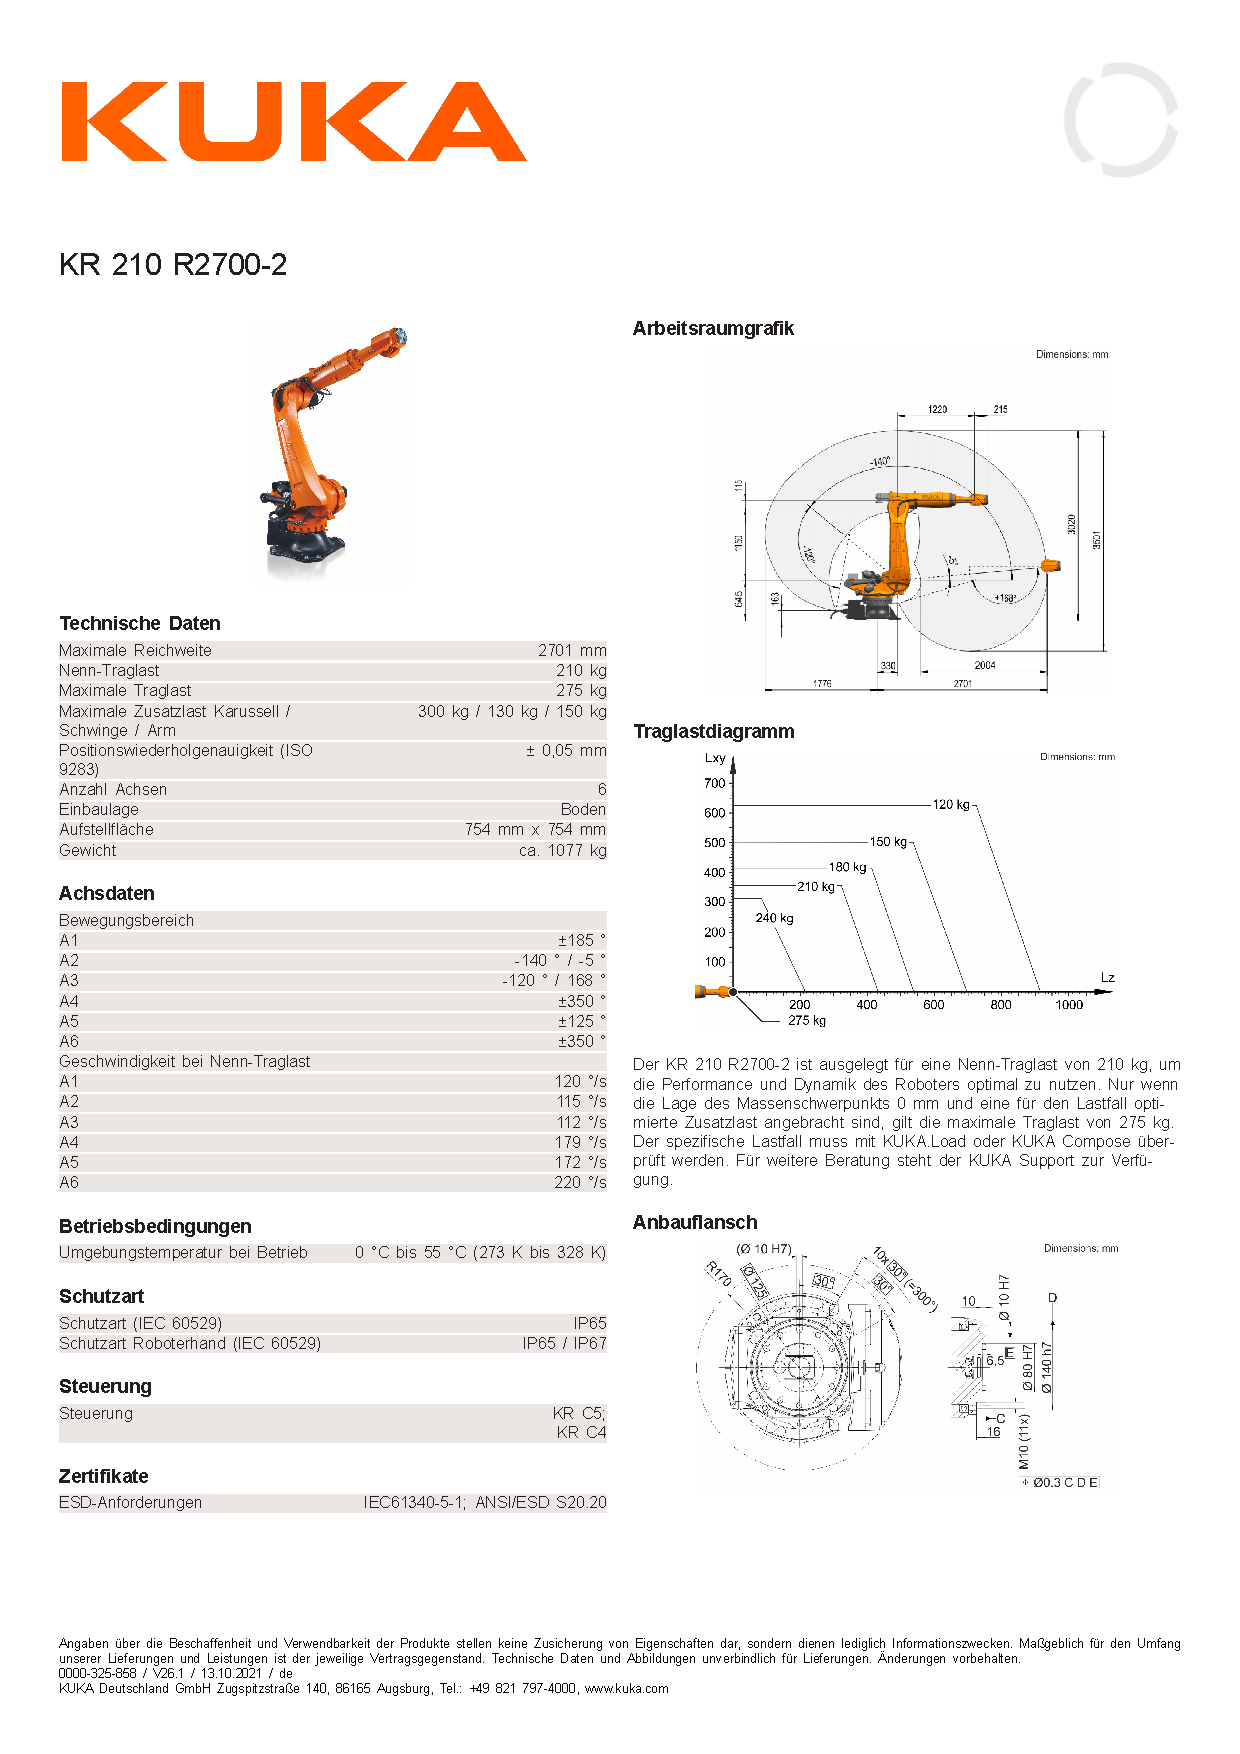
\includepdf[pages=1]{C:/Users/denni/Documents/Bachelorarbeit/BachelorThesis/literature/Anhang/DatenblattKR2102700-2.pdf}
\section{DH-Transformation}
\label{add:dh}
%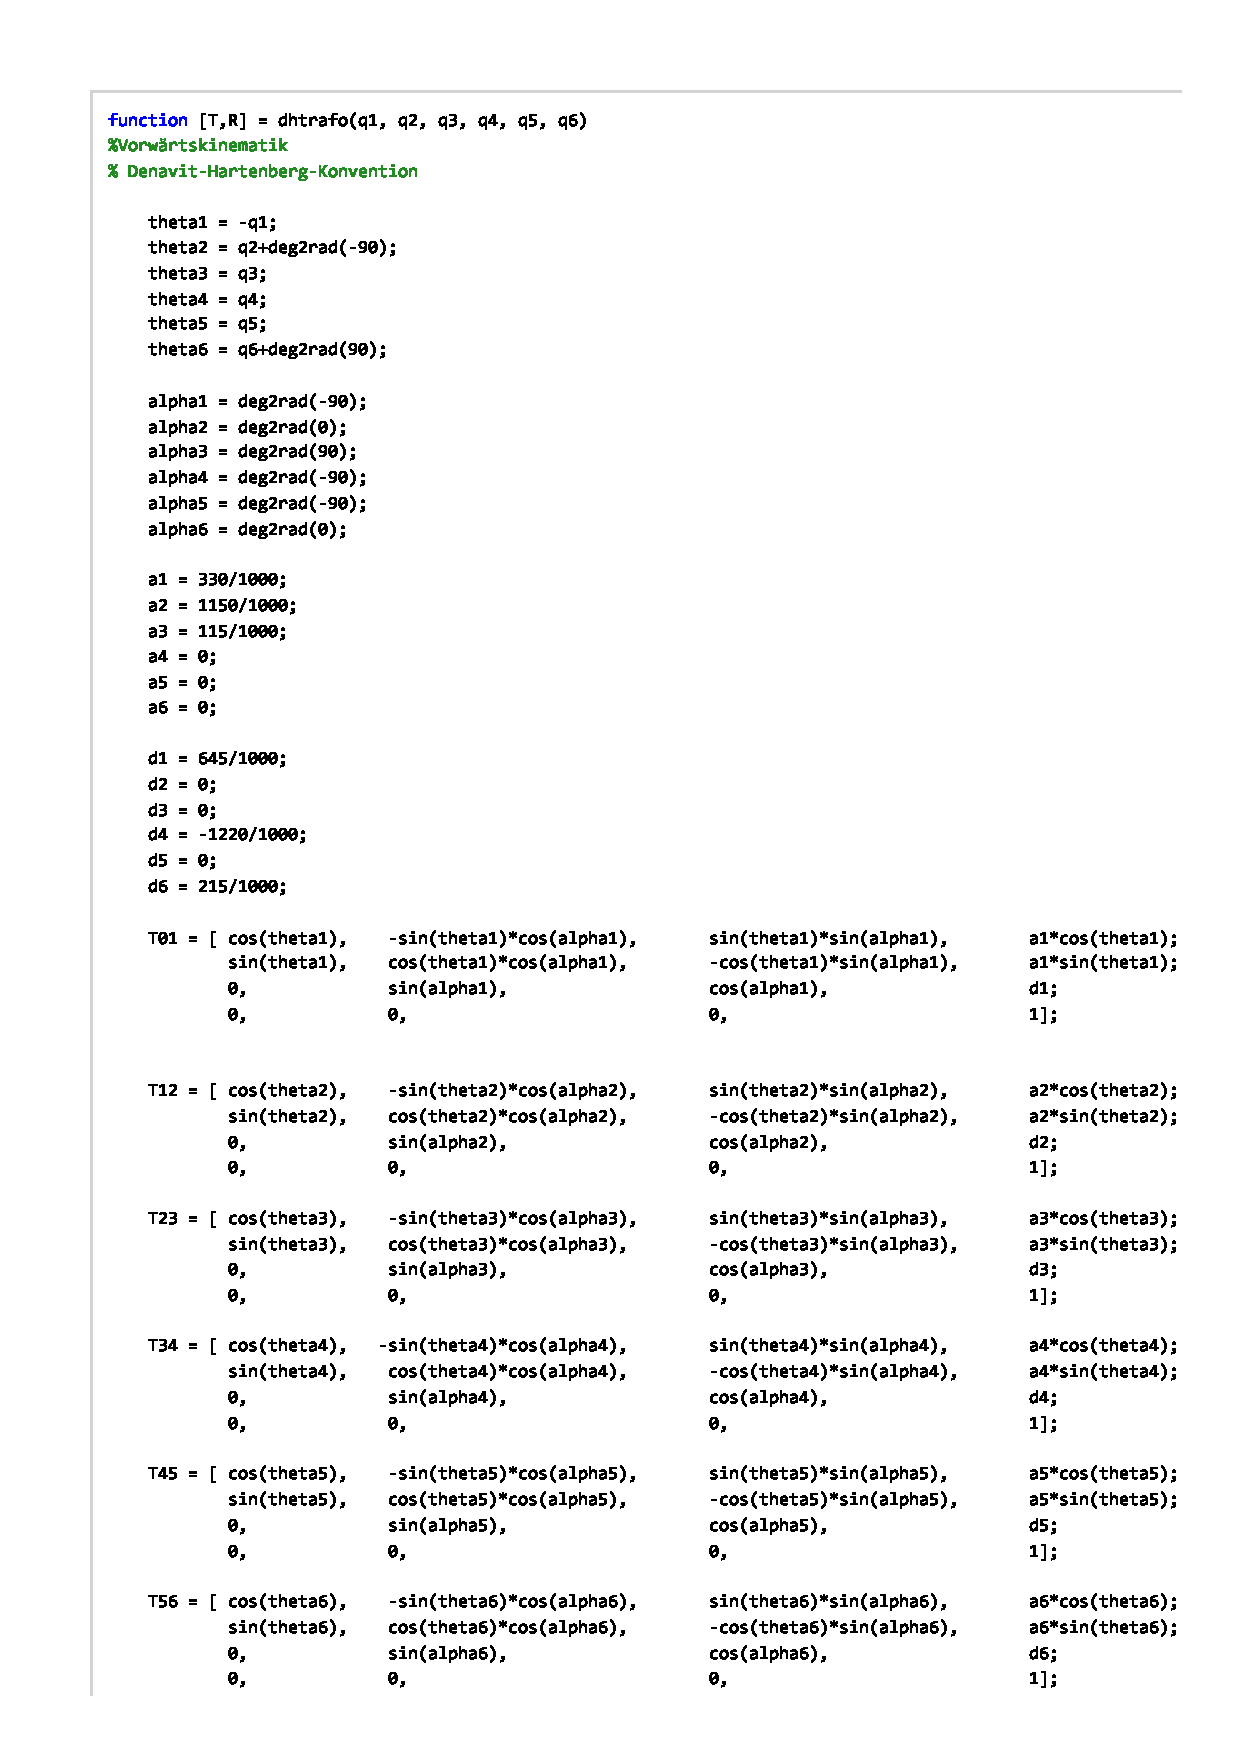
\includepdf[pages=1-2]{C:/Users/denni/Documents/Bachelorarbeit/BachelorThesis/literature/Anhang/dhtrafo_matlab.pdf}
\begin{lstlisting}[language=Matlab]
	function [T,R,R0i] = dhtrafo(q1, q2, q3, q4, q5, q6)
	%Vorwärtskinematik
	% Denavit-Hartenberg-Konvention
	
	theta1 = -q1;
	theta2 = q2+deg2rad(-90);
	theta3 = q3;
	theta4 = q4;
	theta5 = q5;
	theta6 = q6+deg2rad(90);
	
	alpha1 = deg2rad(-90);
	alpha2 = deg2rad(0);
	alpha3 = deg2rad(90);
	alpha4 = deg2rad(-90);
	alpha5 = deg2rad(-90);
	alpha6 = deg2rad(0);
	
	a1 = 330/1000;
	a2 = 1150/1000;
	a3 = 115/1000;
	a4 = 0;
	a5 = 0;
	a6 = 0;
	
	d1 = 645/1000;
	d2 = 0;
	d3 = 0;
	d4 = -1220/1000;
	d5 = 0;
	d6 = 215/1000;
	
	T01 = [ cos(theta1), -sin(theta1)*cos(alpha1), sin(theta1)*sin(alpha1), a1*cos(theta1);
			sin(theta1), cos(theta1)*cos(alpha1), -cos(theta1)*sin(alpha1), a1*sin(theta1);
			0, sin(alpha1), cos(alpha1), d1;
			0, 0, 0, 1];
	
	
	T12 = [ cos(theta2), -sin(theta2)*cos(alpha2), sin(theta2)*sin(alpha2), a2*cos(theta2);
			sin(theta2), cos(theta2)*cos(alpha2), -cos(theta2)*sin(alpha2), a2*sin(theta2);
			0, sin(alpha2), cos(alpha2), d2;
			0, 0, 0, 1];
	
	T23 = [ cos(theta3), -sin(theta3)*cos(alpha3), sin(theta3)*sin(alpha3), a3*cos(theta3);
			sin(theta3), cos(theta3)*cos(alpha3), -cos(theta3)*sin(alpha3), a3*sin(theta3);
			0, sin(alpha3), cos(alpha3), d3;
			0, 0, 0, 1];
	
	T34 = [ cos(theta4), -sin(theta4)*cos(alpha4), sin(theta4)*sin(alpha4), a4*cos(theta4);
			sin(theta4), cos(theta4)*cos(alpha4), -cos(theta4)*sin(alpha4), a4*sin(theta4);
			0, sin(alpha4), 
			 cos(alpha4), d4;
			0, 0, 0, 1];
	
	T45 = [ cos(theta5), -sin(theta5)*cos(alpha5), sin(theta5)*sin(alpha5), a5*cos(theta5);
			sin(theta5), cos(theta5)*cos(alpha5), -cos(theta5)*sin(alpha5), a5*sin(theta5);
			0, sin(alpha5), cos(alpha5), d5;
			0, 0, 0, 1];
	
	T56 = [ cos(theta6), -sin(theta6)*cos(alpha6), sin(theta6)*sin(alpha6), a6*cos(theta6);
			sin(theta6), cos(theta6)*cos(alpha6), -cos(theta6)*sin(alpha6), a6*sin(theta6);
			0, sin(alpha6), cos(alpha6), d6;
			0, 0, 0, 1];
	
	T = cat(3, T01, T12, T23, T34, T45, T56);
	
	R01 = T01(1:3,1:3);
	R12 = T12(1:3,1:3);
	R23 = T23(1:3,1:3);
	R34 = T34(1:3,1:3);
	R45 = T45(1:3,1:3);
	R56 = T56(1:3,1:3);
	
	T02 = T01*T12;
	T03 = T02*T23;
	T04 = T03*T34;
	T05 = T04*T45;
	T06 = T05*T56;
	
	R02 = T02(1:3,1:3);
	R03 = T03(1:3,1:3);
	R04 = T04(1:3,1:3);
	R05 = T05(1:3,1:3);
	R06 = T06(1:3,1:3);
	
	R = cat(3, R01, R12, R23, R34, R45, R56);
	R0i = cat(3, R01, R02, R03, R04, R05, R06);
	
	end
\end{lstlisting}
\label{add:systemparameter}
%
\section{Systemparameter}
Die Massen $m_i$ der Starrkörper $i$ sind dem CAD-Modell des Herstellers entnommen. Hierbei wird angenommen, dass der Werkstoff korrekt zugeordnet ist. 
%
\setlist{noitemsep}
\begin{itemize}
	\item $m_1$ = 535 kg
	\item $m_2$ = 696,3 kg
	\item $m_3$ = 361,6 kg
	\item $m_4$ = 39,676 kg
	\item $m_5$ = 53,619 kg
	\item $m_6$ = 4,528 kg
\end{itemize}
%
Die Trägheitstensoren, werden vom CAD-Modell, bezogen auf das KS$\left\{0\right\}$ vorgegeben. Gleichung \ref{eqn:similarity} zeigt, wie diese einmalig über eine Ähnlichkeitstransformation auf das Körperfeste Koordinatensystem KS$\left\{i\right\}$ transformiert werden. Nachfolgend sind die Trägheitstensoren bezogen auf das KS$\left\{0\right\}$ angegeben. 
%
\setlist{noitemsep}
\begin{itemize}
	\item $I_{1xx} = 17,298~\frac{\text{kg}}{\text{m}^2}$
	\item $I_{1xy} = -2,711~\frac{\text{kg}}{\text{m}^2}$
	\item $I_{1xz} = 1,672~\frac{\text{kg}}{\text{m}^2}$
	\item $I_{1yy} = 32,671~\frac{\text{kg}}{\text{m}^2}$
	\item $I_{1yz} = -0,493~\frac{\text{kg}}{\text{m}^2}$
	\item $I_{1zz} = 29,447~\frac{\text{kg}}{\text{m}^2}$
	\\
	\item $I_{2xx} = 138,135~\frac{\text{kg}}{\text{m}^2}$
	\item $I_{2xy} = -0,012~\frac{\text{kg}}{\text{m}^2}$
	\item $I_{2xz} = 0,387~\frac{\text{kg}}{\text{m}^2}$
	\item $I_{2yy} = 136,664~\frac{\text{kg}}{\text{m}^2}$
	\item $I_{2yz} = 9,231~\frac{\text{kg}}{\text{m}^2}$
	\item $I_{2zz} = 11,838~\frac{\text{kg}}{\text{m}^2}$
	\\
	\item $I_{3xx} = 3,031~\frac{\text{kg}}{\text{m}^2}$
	\item $I_{3xy} = -1,386~\frac{\text{kg}}{\text{m}^2}$
	\item $I_{3xz} = -0,045~\frac{\text{kg}}{\text{m}^2}$
	\item $I_{3yy} = 30,03~\frac{\text{kg}}{\text{m}^2}$
	\item $I_{3yz} = -0,21~\frac{\text{kg}}{\text{m}^2}$
	\item $I_{3zz} = 29,693~\frac{\text{kg}}{\text{m}^2}$
	\\
	\item $I_{4xx} = 0,099~\frac{\text{kg}}{\text{m}^2}$
	\item $I_{4xy} = -0,032~\frac{\text{kg}}{\text{m}^2}$
	\item $I_{4xz} = -0,001~\frac{\text{kg}}{\text{m}^2}$
	\item $I_{4yy} = 0,701~\frac{\text{kg}}{\text{m}^2}$
	\item $I_{4yz} = -9,367\cdot10^{-6}~\frac{\text{kg}}{\text{m}^2}$
	\item $I_{4zz} = 0,698~\frac{\text{kg}}{\text{m}^2}$
	\\
	\item $I_{5xx} = 0,481~\frac{\text{kg}}{\text{m}^2}$
	\item $I_{5xy} = 0,118~\frac{\text{kg}}{\text{m}^2}$
	\item $I_{5xz} = 0.00~\frac{\text{kg}}{\text{m}^2}$
	\item $I_{5yy} = 0,424~\frac{\text{kg}}{\text{m}^2}$
	\item $I_{5yz} = 0,00~\frac{\text{kg}}{\text{m}^2}$
	\item $I_{5zz} = 0,675~\frac{\text{kg}}{\text{m}^2}$
	\\
	\item $I_{6xx} = 0,011~\frac{\text{kg}}{\text{m}^2}$
	\item $I_{6xy} = 5,143\cdot10^{-7}~\frac{\text{kg}}{\text{m}^2}$
	\item $I_{6xz} = -2,003\cdot10^{-6}~\frac{\text{kg}}{\text{m}^2}$
	\item $I_{6yy} = 0,006~\frac{\text{kg}}{\text{m}^2}$
	\item $I_{6yz} = 1,220\cdot10^{07}~\frac{\text{kg}}{\text{m}^2}$
	\item $I_{6zz} = 0,006~\frac{\text{kg}}{\text{m}^2}$
\end{itemize}
%
Nachfolgend ist die Lage der Massenschwerpunkte $C_i^0$ im KS$\left\{0\right\}$ angegeben. 
% 
\begin{itemize}
	\item $r_{0,C_1}^0$ = $\left[-30,103,~441,~452,213\right]$ mm
	\item $r_{0,C_2}^0$ = $\left[330,979,~-222,585,~1094,239\right]$ mm
	\item $r_{0,C_3}^0$ = $\left[705,894,~-8,126,~1908,436\right]$ mm
	\item $r_{0,C_4}^0$ = $\left[1383,185,~4,492,~1909,983\right]$ mm
	\item $r_{0,C_5}^0$ = $\left[1601,767,~33,833,~1909,955\right]$ mm
	\item $r_{0,C_6}^0$ = $\left[1743,222,~-0,007,~1910 051\right]$ mm
\end{itemize}
%
Die Getriebeübersetzung ist der Datei Machine Data (MADA) der Robotersteuerung entnommen.
%
\begin{itemize}
	\item $i_1 = -\frac{7}{1798}$
	\item $i_2 = -\frac{17}{4576}$
	\item $i_3 = \frac{3}{754}$
	\item $i_4 = -\frac{55}{10387}$
	\item $i_5 = -\frac{483}{91834}$
	\item $i_6 = \frac{49400}{6485103}$
\end{itemize}
 %
Nachfolgend ist die Umsetzung der Parameter Transformation via MATLAB\textsuperscript{\textregistered} gezeigt. 
%
%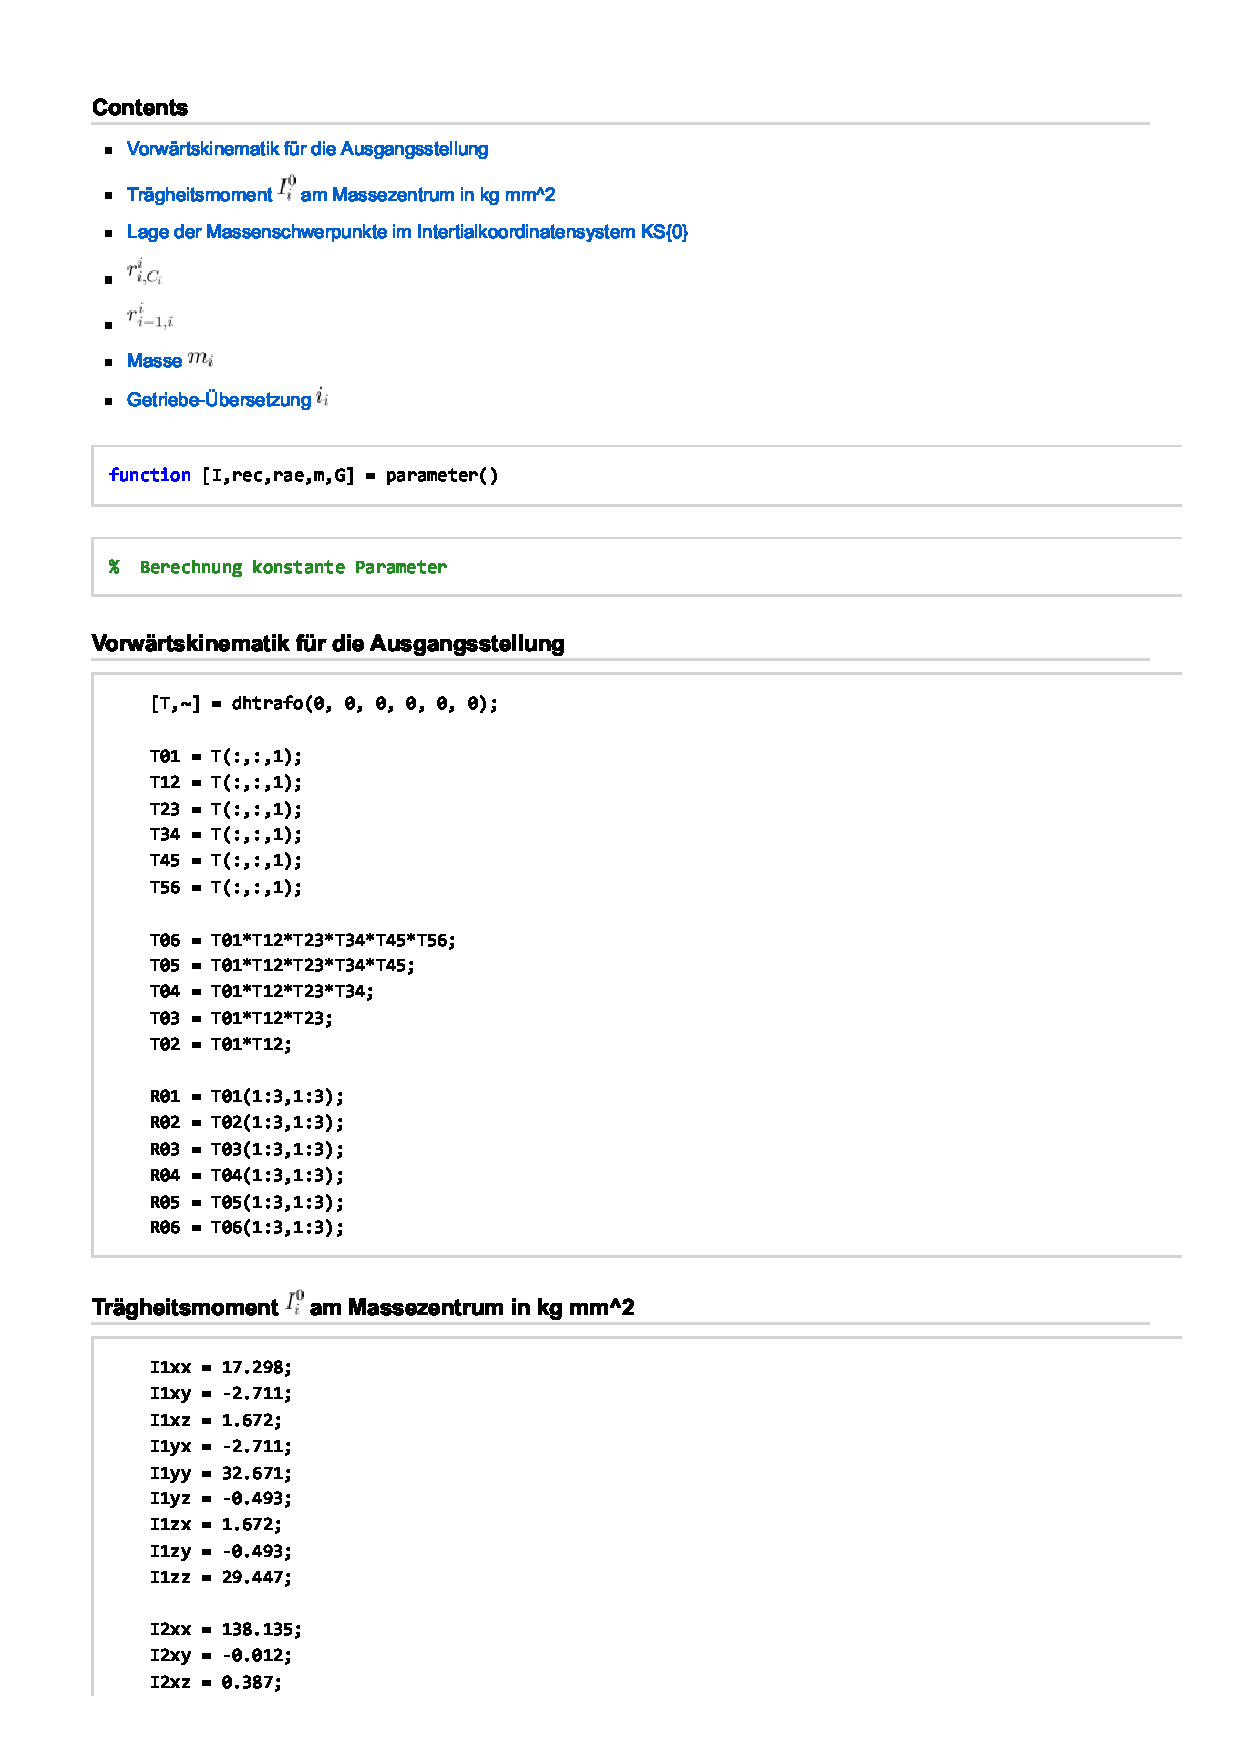
\includepdf[pages=1-4]{C:/Users/denni/Documents/Bachelorarbeit/BachelorThesis/literature/Anhang/parameter_matlab.pdf}
\subsection*{Funktionalitäten}
%
\begin{itemize}
	\setlength{\itemsep}{-1ex}
	\item Vorwärtskinematik für die Ausgangsstellung
	\item Trägheitsmoment $I^{0}_i$ am Massezentrum in kg mm\^{}2
	\item Lage der Massenschwerpunkte im Intertialkoordinatensystem KS\{0\}
	\item $r^{i}_{i,C_i}$
	\item $r^{i}_{i-1,i}$
	\item Masse $m_i$
	\item Getriebe-Übersetzung $i_i$
\end{itemize}
\begin{lstlisting}
	function [I,rec,rae,m,G] = parameter()
	% Berechnung konstante Parameter
\end{lstlisting}
%
\subsection*{Vorwärtskinematik für die Ausgangsstellung}
%
\begin{lstlisting}
	[T,~,~] = dhtrafo(0, 0, 0, 0, 0, 0);
	
	T01 = T(:,:,1);
	T12 = T(:,:,2);
	T23 = T(:,:,3);
	T34 = T(:,:,4);
	T45 = T(:,:,5);
	T56 = T(:,:,6);
	T06 = T01*T12*T23*T34*T45*T56;
	T05 = T01*T12*T23*T34*T45;
	T04 = T01*T12*T23*T34;
	T03 = T01*T12*T23;
	T02 = T01*T12;
	
	R01 = T01(1:3,1:3);
	R02 = T02(1:3,1:3);
	R03 = T03(1:3,1:3);
	R04 = T04(1:3,1:3);
	R05 = T05(1:3,1:3);
	R06 = T06(1:3,1:3);
\end{lstlisting}
%
\subsection*{Trägheitsmoment $I^{0}_i$ am Massezentrum in kg mm\^{}2}
%
\begin{lstlisting}
	I1xx = 17.298;
	I1xy = -2.711;
	I1xz = 1.672;
	I1yx = -2.711;
	I1yy = 32.671;
	I1yz = -0.493;
	I1zx = 1.672;
	I1zy = -0.493;
	I1zz = 29.447;
	
	I2xx = 138.135;
	I2xy = -0.012;
	I2xz = 0.387;
	I2yx = -0.012;
	I2yy = 136.664;
	I2yz = 9.231;
	I2zx = 0.387;
	I2zy = 9.231;
	I2zz = 11.838;
	
	I3xx = 3.031;
	I3xy = -1.386;
	I3xz = -0.045;
	I3yx = -1.386;
	I3yy = 30.03;
	I3yz = -0.21;
	I3zx = -0.045;
	I3zy = -0.21;
	I3zz = 29.693;
	
	I4xx = 0.099;
	I4xy = -0.032;
	I4xz = -0.001;
	I4yx = -0.032;
	I4yy = 0.701;
	I4yz = -9.367E-06;
	I4zx = -0.001;
	I4zy = -9.367E-06;
	I4zz = 0.698;
	
	I5xx = 0.481;
	I5xy = 0.118;
	I5xz = 0.00;
	I5yx = 0.118;
	I5yy = 0.424;
	I5yz = 0.00;
	I5zx = 0.00;
	I5zy = 0.00;
	I5zz = 0.675;
	
	I6xx = 0.011;
	I6xy = 5.143E-07;
	I6xz = -2.003E-06;
	I6yx = 5.143E-07;
	I6yy = 0.006;
	I6yz = 1.220E-07;
	I6zx = -2.003E-06;
	I6zy = 1.220E-07;
	I6zz = 0.006;
	
	% Ähnlichkeitstransformation zur Umrechung in die Körperfesten
	% Koordinatensysteme
	
	I1base = [ I1xx, I1xy, I1xz;
					I1yx, I1yy, I1yz;
					I1zx, I1zy, I1zz];
	
	I1 = R01'*I1base*R01;
	
	I2base = [ I2xx, I2xy, I2xz;
					I2yx, I2yy, I2yz;
					I2zx, I2zy, I2zz];
	
	I2 = R02'*I2base*R02;
	
	I3base = [ I3xx, I3xy, I3xz;
					I3yx, I3yy, I3yz;
					I3zx, I3zy, I3zz];
	
	I3 = R03'*I3base*R03;
	
	I4base = [ I4xx, I4xy, I4xz;
					I4yx, I4yy, I4yz;
					I4zx, I4zy, I4zz];
					
	I4 = R04'*I4base*R04;
	
	I5base = [ I5xx, I5xy, I5xz;
					I5yx, I5yy, I5yz;
					I5zx, I5zy, I5zz];
	
	I5 = R05'*I5base*R05;
	
	I6base = [ I6xx, I6xy, I6xz;
					I6yx, I6yy, I6yz;
					I6zx, I6zy, I6zz];
	
	I6 = R06'*I6base*R06;
	
	I = cat(3,I1,I2,I3,I4,I5,I6);
\end{lstlisting}
%
\subsection*{Lage der Massenschwerpunkte im Intertialkoordinatensystem KS\{0\}}
%
\begin{lstlisting}
	com1 = [-30.103; 4.41; 452.213]/1000;
	com2 = [330.979; -222.585; 1094.239]/1000;
	com3 = [705.894; -8.126; 1908.436]/1000;
	com4 = [1383.185; 4.492; 1909.983]/1000;
	com5 = [1601.767; 33.833; 1909.955]/1000;
	com6 = [1743.222; -0.007; 1910.051]/1000;
\end{lstlisting}
%
\subsection*{$r^{i}_{i,C_i}$}
%
\begin{lstlisting}
	r1e_c1 = (T01)\[com1;1]; r1e_c1 = r1e_c1(1:3,1);
	r2e_c2 = (T02)\[com2;1]; r2e_c2 = r2e_c2(1:3,1);
	r3e_c3 = (T03)\[com3;1]; r3e_c3 = r3e_c3(1:3,1);
	r4e_c4 = (T04)\[com4;1]; r4e_c4 = r4e_c4(1:3,1);
	r5e_c5 = (T05)\[com5;1]; r5e_c5 = r5e_c5(1:3,1);
	r6e_c6 = (T06)\[com6;1]; r6e_c6 = r6e_c6(1:3,1);
	
	rec= cat(3, r1e_c1, r2e_c2, r3e_c3, r4e_c4, r5e_c5, r6e_c6);
\end{lstlisting}
%
\subsection*{$r^{i}_{i-1,i}$}
%
\begin{lstlisting}
	r1a_e = -inv(T01); r1a_e = r1a_e(1:3,4);
	r2a_e = -inv(T12); r2a_e = r2a_e(1:3,4);
	r3a_e = -inv(T23); r3a_e = r3a_e(1:3,4);
	r4a_e = -inv(T34); r4a_e = r4a_e(1:3,4);
	r5a_e = -inv(T45); r5a_e = r5a_e(1:3,4);
	r6a_e = -inv(T56); r6a_e = r6a_e(1:3,4);
	
	rae = cat(3, r1a_e, r2a_e, r3a_e, r4a_e, r5a_e, r6a_e);
\end{lstlisting}
%
\subsection*{Masse $m_i$}
%
\begin{lstlisting}
	m1 = 535;
	m2 = 696.3;
	m3 = 361.6; % +65.3 kg für die Schlauchpaket-Halterung +50 kg für die Antriebe 4 und 5;
	m4 = 39.676;
	m5 = 53.619;
	m6 = 4.528;
	m = [m1,m2,m3,m4,m5,m6];
\end{lstlisting}
%
\subsection*{Getriebe-Übersetzung $i_i$}
%
\begin{lstlisting}
	i1 = -7/1798;
	i2 = -17/4576;
	i3 = 3/754;
	i4 = -55/10387;
	i5 = -483/91834;
	i6 = 49400/6485103;
	G = [i1, i2, i3, i4, i5, i6];
\end{lstlisting}
\begin{lstlisting}
	end
\end{lstlisting}
%
\section{RNEA}
\label{add:rnea}
%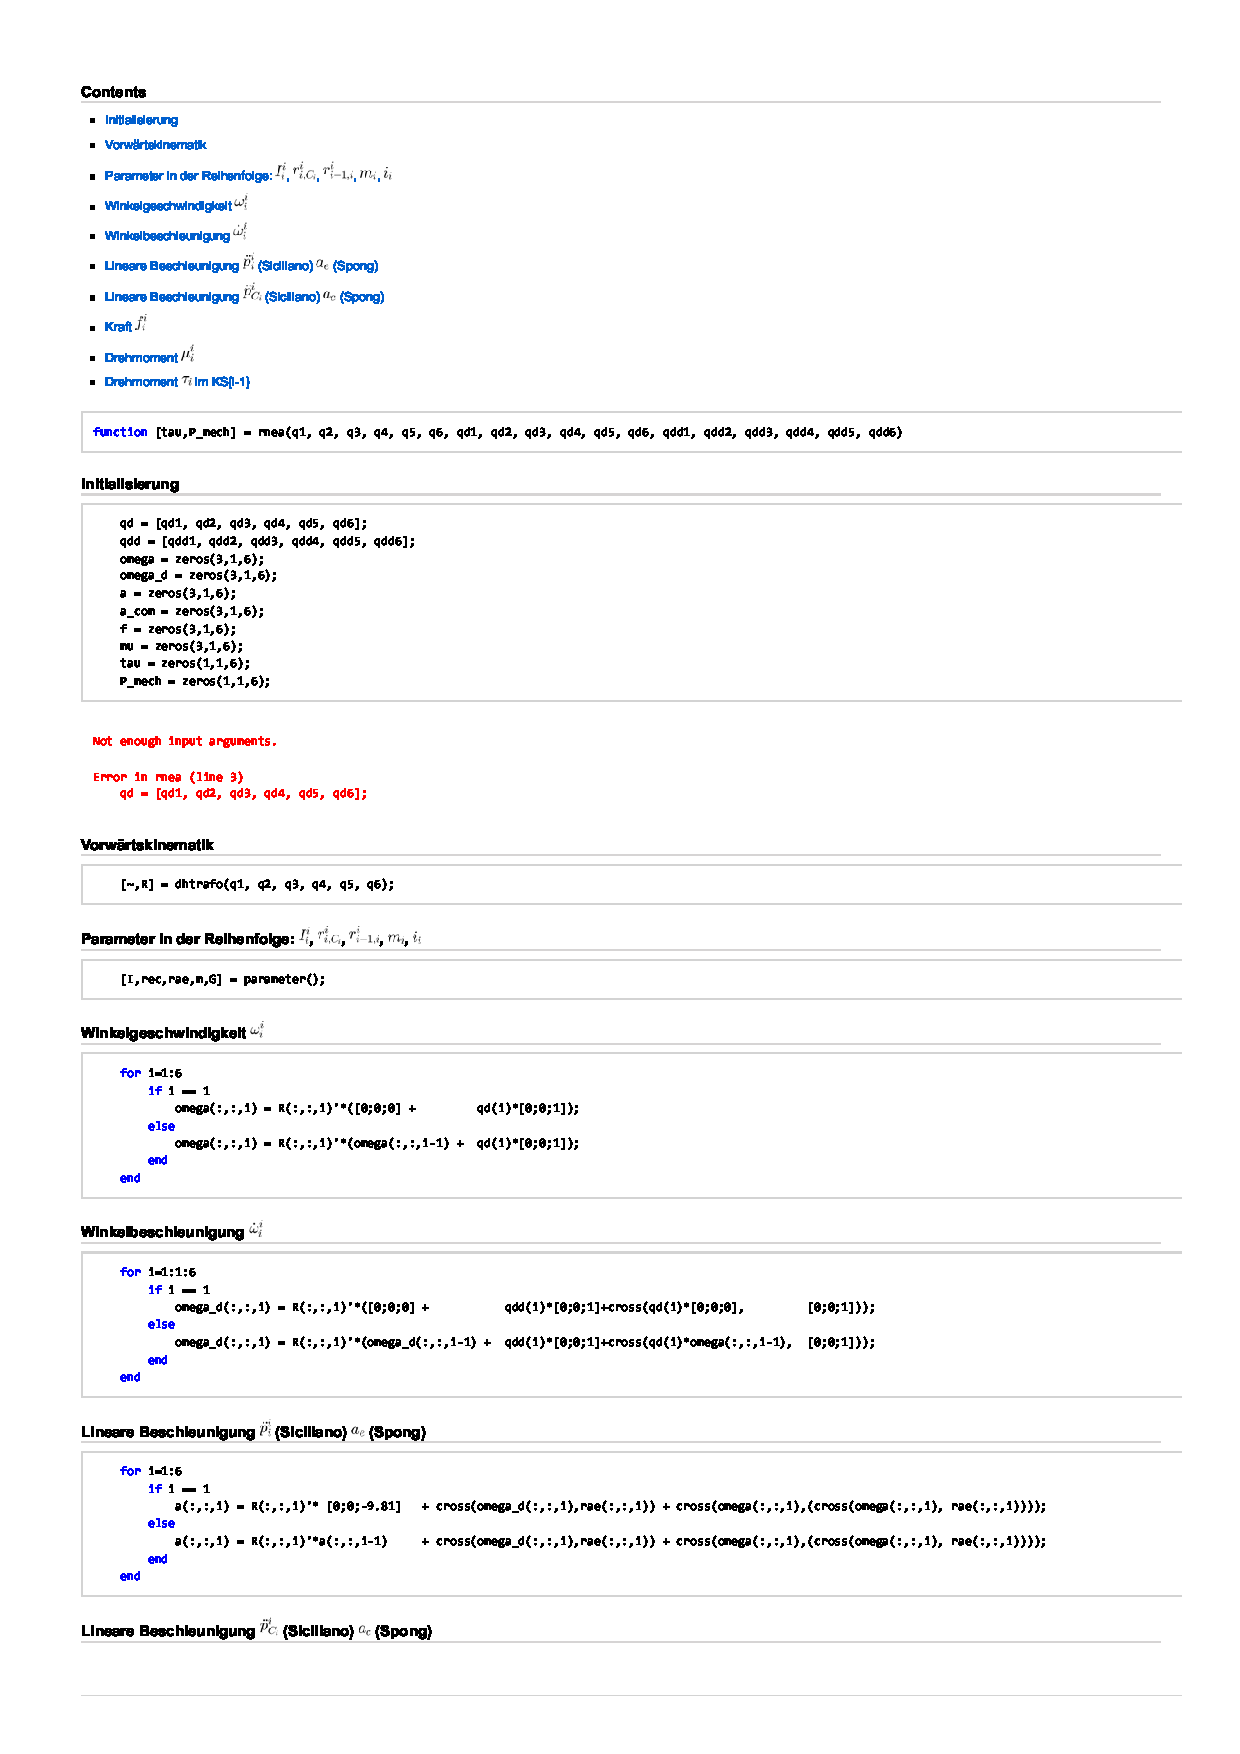
\includepdf[pages=1-2]{C:/Users/denni/Documents/Bachelorarbeit/BachelorThesis/literature/Anhang/rnea_matlab.pdf}
\subsection*{Funktionalitäten}
%
\begin{itemize}
	\setlength{\itemsep}{-1ex}
	\item Initialisierung
	\item Vorwärtskinematik
	\item Parameter in der Reihenfolge: $I^{i}_{i}$, $r^{i}_{i,C_i}$, $r^{i}_{i-1,i}$, $m_i$, $i_i$
	\item Winkelgeschwindigkeit $\omega^{i}_i$
	\item Winkelbeschleunigung $\dot\omega^{i}_i$
	\item Lineare Beschleunigung $\ddot p^{i}_i$ (Siciliano) $a_e$ (Spong)
	\item Lineare Beschleunigung $\ddot p^{i}_{C_i}$ (Siciliano) $a_c$ (Spong)
	\item Gewichtsausgleich
	\item Kraft $f^{i}_i$
	\item Drehmoment $\mu^{i}_i$
	\item Drehmoment $\tau_i$ im KS\{i-1\}
\end{itemize}
\begin{lstlisting}
	function [tau,P_mech] = rnea(q1, q2, q3, q4, q5, q6, qd1, qd2, qd3, qd4, qd5, qd6, qdd1, qdd2, qdd3, qdd4, qdd5, qdd6)
\end{lstlisting}
%
\subsection*{Initialisierung}
%
\begin{lstlisting}
	qd = [qd1, qd2, qd3, qd4, qd5, qd6];
	qdd = [qdd1, qdd2, qdd3, qdd4, qdd5, qdd6];
	omega = zeros(3,1,6);
	omega_d = zeros(3,1,6);
	a = zeros(3,1,6);
	a_com = zeros(3,1,6);
	f = zeros(3,1,6);
	mu = zeros(3,1,6);
	tau = zeros(1,1,6);
	P_mech = zeros(1,1,6);
\end{lstlisting}
%
\subsection*{Vorwärtskinematik}
%
\begin{lstlisting}
	[~,R,R0i] = dhtrafo(q1, q2, q3, q4, q5, q6);
\end{lstlisting}
%
\subsection*{Parameter in der Reihenfolge: $I^{i}_{i}$, $r^{i}_{i,C_i}$, $r^{i}_{i-1,i}$, $m_i$, $i_i$}
%
\begin{lstlisting}
	[I,rec,rae,m,G] = parameter();
\end{lstlisting}
%
\subsection*{Winkelgeschwindigkeit $\omega^{i}_i$}
%
\begin{lstlisting}
	for i=1:6
	if i == 1
	omega(:,:,i) = R(:,:,i)'*([0;0;0] + qd(i)*[0;0;1]);
	else
	omega(:,:,i) = R(:,:,i)'*(omega(:,:,i-1) + qd(i)*[0;0;1]);
	end
	end
\end{lstlisting}
%
\subsection*{Winkelbeschleunigung $\dot\omega^{i}_i$}
%
\begin{lstlisting}
	for i=1:1:6
	if i == 1
	omega_d(:,:,i) = R(:,:,i)'*([0;0;0] + qdd(i)*[0;0;1]+cross(qd(i)*[0;0;0], [0;0;1]));
	else
	omega_d(:,:,i) = R(:,:,i)'*(omega_d(:,:,i-1) + qdd(i)*[0;0;1]+cross(qd(i)*omega(:,:,i-1), [0;0;1]));
	end
	end
\end{lstlisting}
%
\subsection*{Lineare Beschleunigung $\ddot p^{i}_i$ (Siciliano) $a_e$ (Spong)}
%
\begin{lstlisting}
	for i=1:6
	if i == 1
	a(:,:,i) = R(:,:,i)'* [0;0;-9.81] + cross(omega_d(:,:,i),rae(:,:,i)) + cross(omega(:,:,i),(cross(omega(:,:,i), rae(:,:,i))));
	else
	a(:,:,i) = R(:,:,i)'*a(:,:,i-1) + cross(omega_d(:,:,i),rae(:,:,i)) + cross(omega(:,:,i),(cross(omega(:,:,i), rae(:,:,i))));
	end
	end
\end{lstlisting}
%
\subsection*{Lineare Beschleunigung $\ddot p^{i}_{C_i}$ (Siciliano) $a_c$ (Spong)}
%
\begin{lstlisting}
	for i=1:1:6
	a_com(:,:,i) = a(:,:,i) + cross(omega_d(:,:,i),rec(:,:,i)) + cross(omega(:,:,i),(cross(omega(:,:,i), rec(:,:,i))));
	end
\end{lstlisting}
%
\subsection*{Gewichtsausgleich}
%
\begin{lstlisting}
	F_gravity = zeros(3, 1, 6); % Vektor für die Gewichtskraft
	for i = 1:6
	F_gravity(:,:,i) = m(i) * [0; 0; -9.81]; % Gewichtskraft in Weltkoordinaten
	F_gravity(:,:,i) = R0i(:,:,i)' * F_gravity(:,:,i); % Gewichtskraft ins Körpersystem transformieren
	end
	
	for i = 3:-1:2
	if i == 3
	fgrav(:,:,i) = eye(3)*F_gravity(:,:,i);
	mugrav(:,:,i) = cross(-fgrav(:,:,i),(rae(:,:,i)+rec(:,:,i)));
	else
	fgrav(:,:,i) = R(:,:,i+1)*fgrav(:,:,i+1) + eye(3)*F_gravity(:,:,i);
	mugrav(:,:,i) = cross(-fgrav(:,:,i),(rae(:,:,i)+rec(:,:,i))) + R(:,:,i+1)*mugrav(:,:,i+1) + R(:,:,i+1)*cross(fgrav(:,:,i+1), rec(:,:,i));
	end
	end
\end{lstlisting}
%
\subsection*{Kraft $f^{i}_i$}
%
\begin{lstlisting}
	for i = 6:-1:1
	if i == 6
	f(:,:,i) = eye(3)*[0;0;0] + m(i)*a_com(:,:,i);
	elseif i == 2
	f(:,:,i) = R(:,:,i+1)*f(:,:,i+1) + m(i)*a_com(:,:,i);
	else
	f(:,:,i) = R(:,:,i+1)*f(:,:,i+1) + m(i)*a_com(:,:,i);
	end
	end
\end{lstlisting}
%
\subsection*{Drehmoment $\mu^{i}_i$}
%
\begin{par}
	Übertragung des Drehmoments von der zweiten auf die ersten Achse ist zu Null gesetzt
\end{par} \vspace{1em}
\begin{lstlisting}
	for i = 6:-1:1
	if i == 6
	mu(:,:,i) = cross(-f(:,:,i),(rae(:,:,i)+rec(:,:,i))) + eye(3)*[0;0;0] + eye(3)*cross([0;0;0], rec(:,:,i)) + I(:,:,i)*omega_d(:,:,i) + cross(omega(:,:,i),(I(:,:,i)*omega(:,:,i)));
	elseif i == 2
	mu(:,:,i) = cross(-f(:,:,i),(rae(:,:,i)+rec(:,:,i))) + R(:,:,i+1)*mu(:,:,i+1) + R(:,:,i+1)*cross(f(:,:,i+1), rec(:,:,i)) + I(:,:,i)*omega_d(:,:,i) + cross(omega(:,:,i),(I(:,:,i)*omega(:,:,i)))- mugrav(:,:,i);
	elseif i == 1
	mu(:,:,i) = cross(-f(:,:,i),(rae(:,:,i)+rec(:,:,i))) + R(:,:,i+1)*cross(f(:,:,i+1), rec(:,:,i)) + I(:,:,i)*omega_d(:,:,i) + cross(omega(:,:,i),(I(:,:,i)*omega(:,:,i)));
	else
	mu(:,:,i) = cross(-f(:,:,i),(rae(:,:,i)+rec(:,:,i))) + R(:,:,i+1)*mu(:,:,i+1) + R(:,:,i+1)*cross(f(:,:,i+1), rec(:,:,i)) + I(:,:,i)*omega_d(:,:,i) + cross(omega(:,:,i),(I(:,:,i)*omega(:,:,i)));
	end
	end
\end{lstlisting}
%
\subsection*{Drehmoment $\tau_i$ im KS\{i-1\}}
%
\begin{lstlisting}
	for i = 1:1:6
	tau(i) = transpose(mu(:,:,i)) * transpose(R(:,:,i))*[0;0;1];%* G(i)
	end
	for i = 1:1:6
	P_mech(i) = tau(i)*qd(i);%/G(i);
	end
\end{lstlisting}
\begin{lstlisting}
	end
\end{lstlisting}
\section{Bahnplanung}
\label{add:traj}
%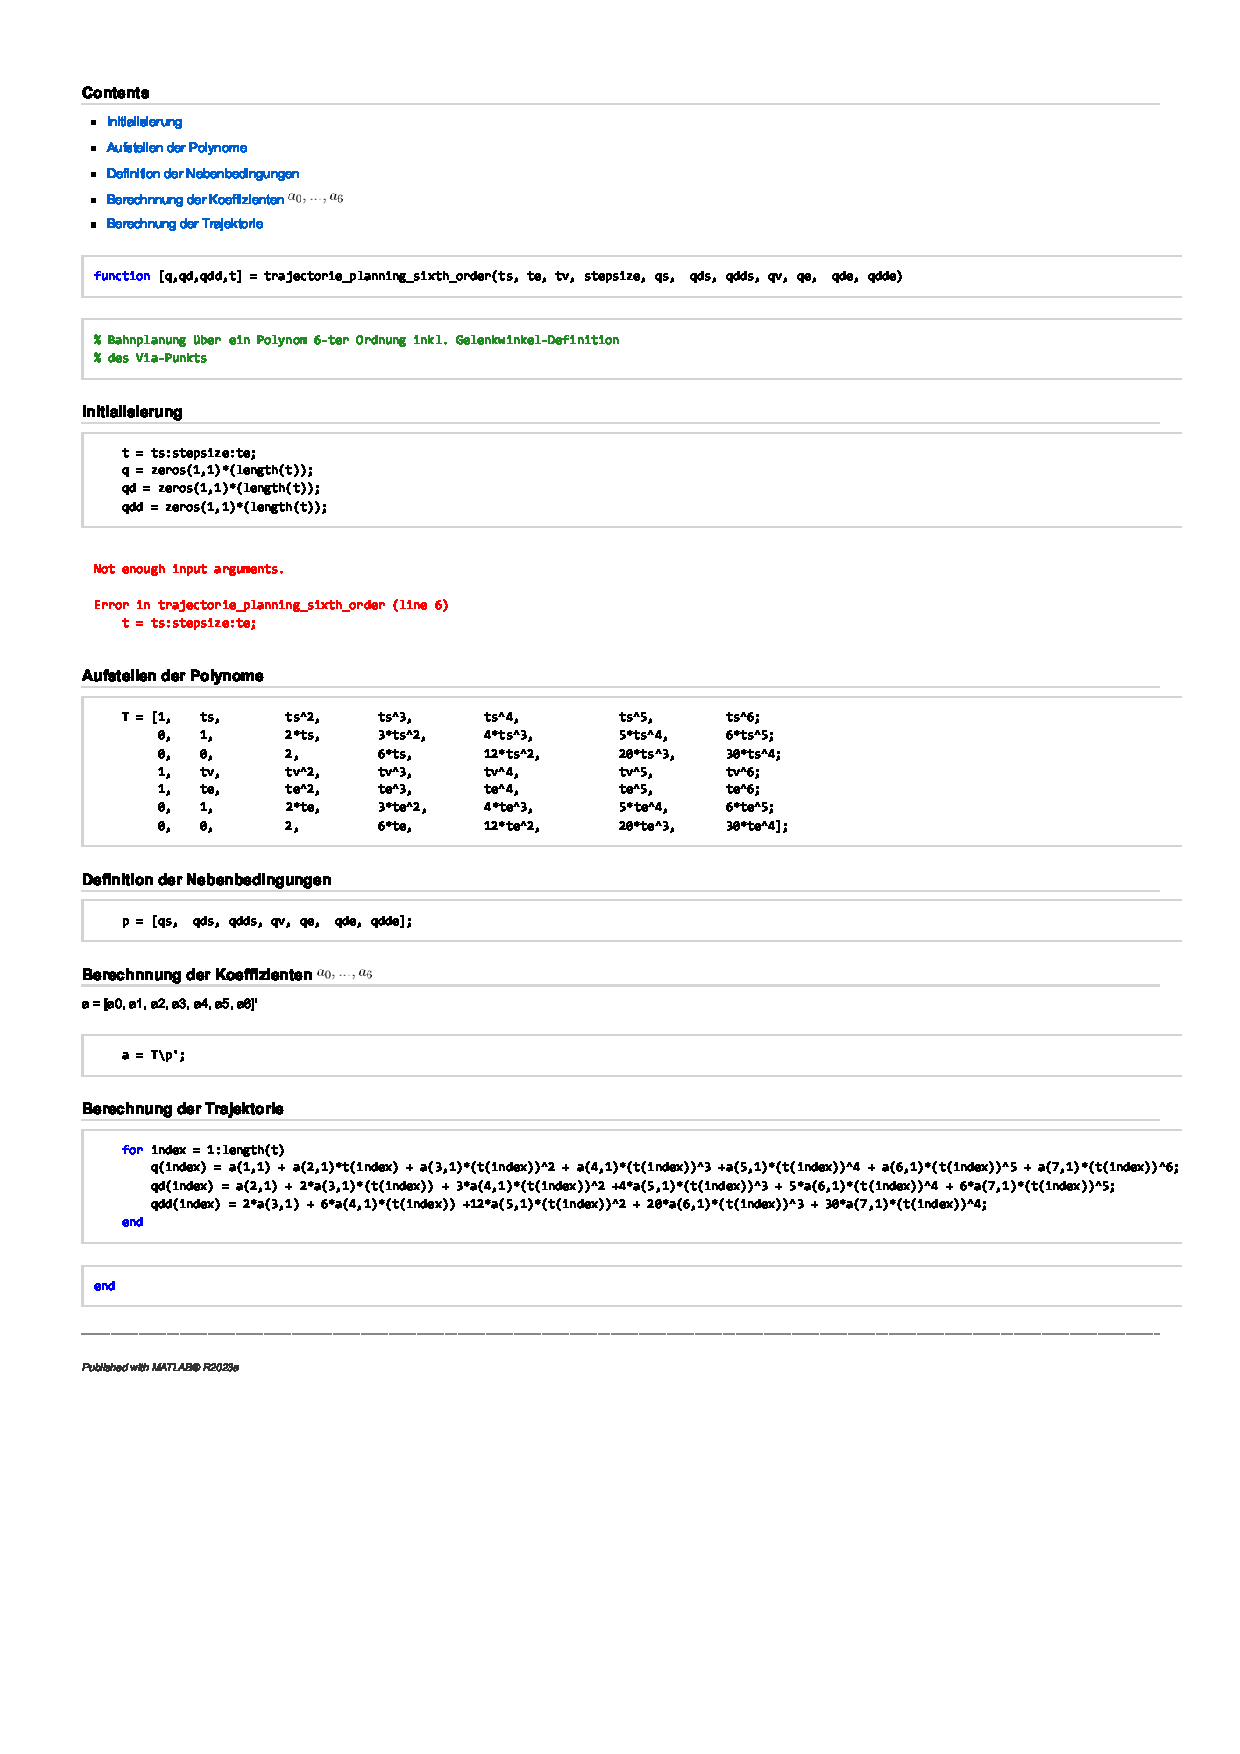
\includepdf[pages=1]{C:/Users/denni/Documents/Bachelorarbeit/BachelorThesis/literature/Anhang/trajectorie_planning_sixth_order_matlab.pdf}
\subsection*{Funktionalitäten}
%
\begin{itemize}
	\setlength{\itemsep}{-1ex}
	\item Initialisierung
	\item Aufstellen der Polynome
	\item Definition der Nebenbedingungen
	\item Berechnnung der Koeffizienten $a_0,...,a_6$
	\item Berechnung der Trajektorie
\end{itemize}
\begin{lstlisting}
	function [q,qd,qdd,t] = trajectorie_planning_sixth_order(ts, te, tv, stepsize, qs, qds, qdds, qv, qe, qde, qdde)
\end{lstlisting}
\begin{lstlisting}
	% Bahnplanung über ein Polynom 6-ter Ordnung inkl. Gelenkwinkel-Definition
	% des Via-Punkts
\end{lstlisting}
%
\subsection*{Initialisierung}
%
\begin{lstlisting}
	t = ts:stepsize:te;
	q = zeros(1,1)*(length(t));
	qd = zeros(1,1)*(length(t));
	qdd = zeros(1,1)*(length(t));
\end{lstlisting}
%
\subsection*{Aufstellen der Polynome}
%
\begin{lstlisting}
	T = [ 1, ts, ts^2, ts^3, ts^4, ts^5, ts^6;
	0, 1, 2*ts, 3*ts^2, 4*ts^3, 5*ts^4, 6*ts^5;
	0, 0, 2, 6*ts, 12*ts^2, 20*ts^3, 30*ts^4;
	1, tv, tv^2, tv^3, tv^4, tv^5, tv^6;
	1, te, te^2, te^3, te^4, te^5, te^6;
	0, 1, 	 2*te, 3*te^2, 4*te^3, 5*te^4, 6*te^5;
	0, 0, 2, 6*te, 12*te^2, 20*te^3, 30*te^4];
\end{lstlisting}
%
\subsection*{Definition der Nebenbedingungen}
%
\begin{lstlisting}
	p = [qs, qds, qdds, qv, qe, qde, qdde];
\end{lstlisting}
%
\subsection*{Berechnnung der Koeffizienten $a_0,...,a_6$}
%
\begin{par}
	a = [a0, a1, a2, a3, a4, a5, a6]'
\end{par} \vspace{1em}
\begin{lstlisting}
	a = T\p';
\end{lstlisting}
%
\subsection*{Berechnung der Trajektorie}
%
\begin{lstlisting}
	for index = 1:length(t)
	q(index) = a(1,1) + a(2,1)*t(index) + a(3,1)*(t(index))^2 + a(4,1)*(t(index))^3 +a(5,1)*(t(index))^4 + a(6,1)*(t(index))^5 + a(7,1)*(t(index))^6;
	qd(index) = a(2,1) + 2*a(3,1)*(t(index)) + 3*a(4,1)*(t(index))^2 +4*a(5,1)*(t(index))^3 + 5*a(6,1)*(t(index))^4 + 6*a(7,1)*(t(index))^5;
	qdd(index) = 2*a(3,1) + 6*a(4,1)*(t(index)) +12*a(5,1)*(t(index))^2 + 20*a(6,1)*(t(index))^3 + 30*a(7,1)*(t(index))^4;
	end
\end{lstlisting}
\begin{lstlisting}
	end
\end{lstlisting}
%
\setcounter{chapter}{2}
\setcounter{section}{5}
\setcounter{table}{0}
\setcounter{figure}{0}
%
\section{Testsimulation Bahnplanung}
\label{add:sim}
%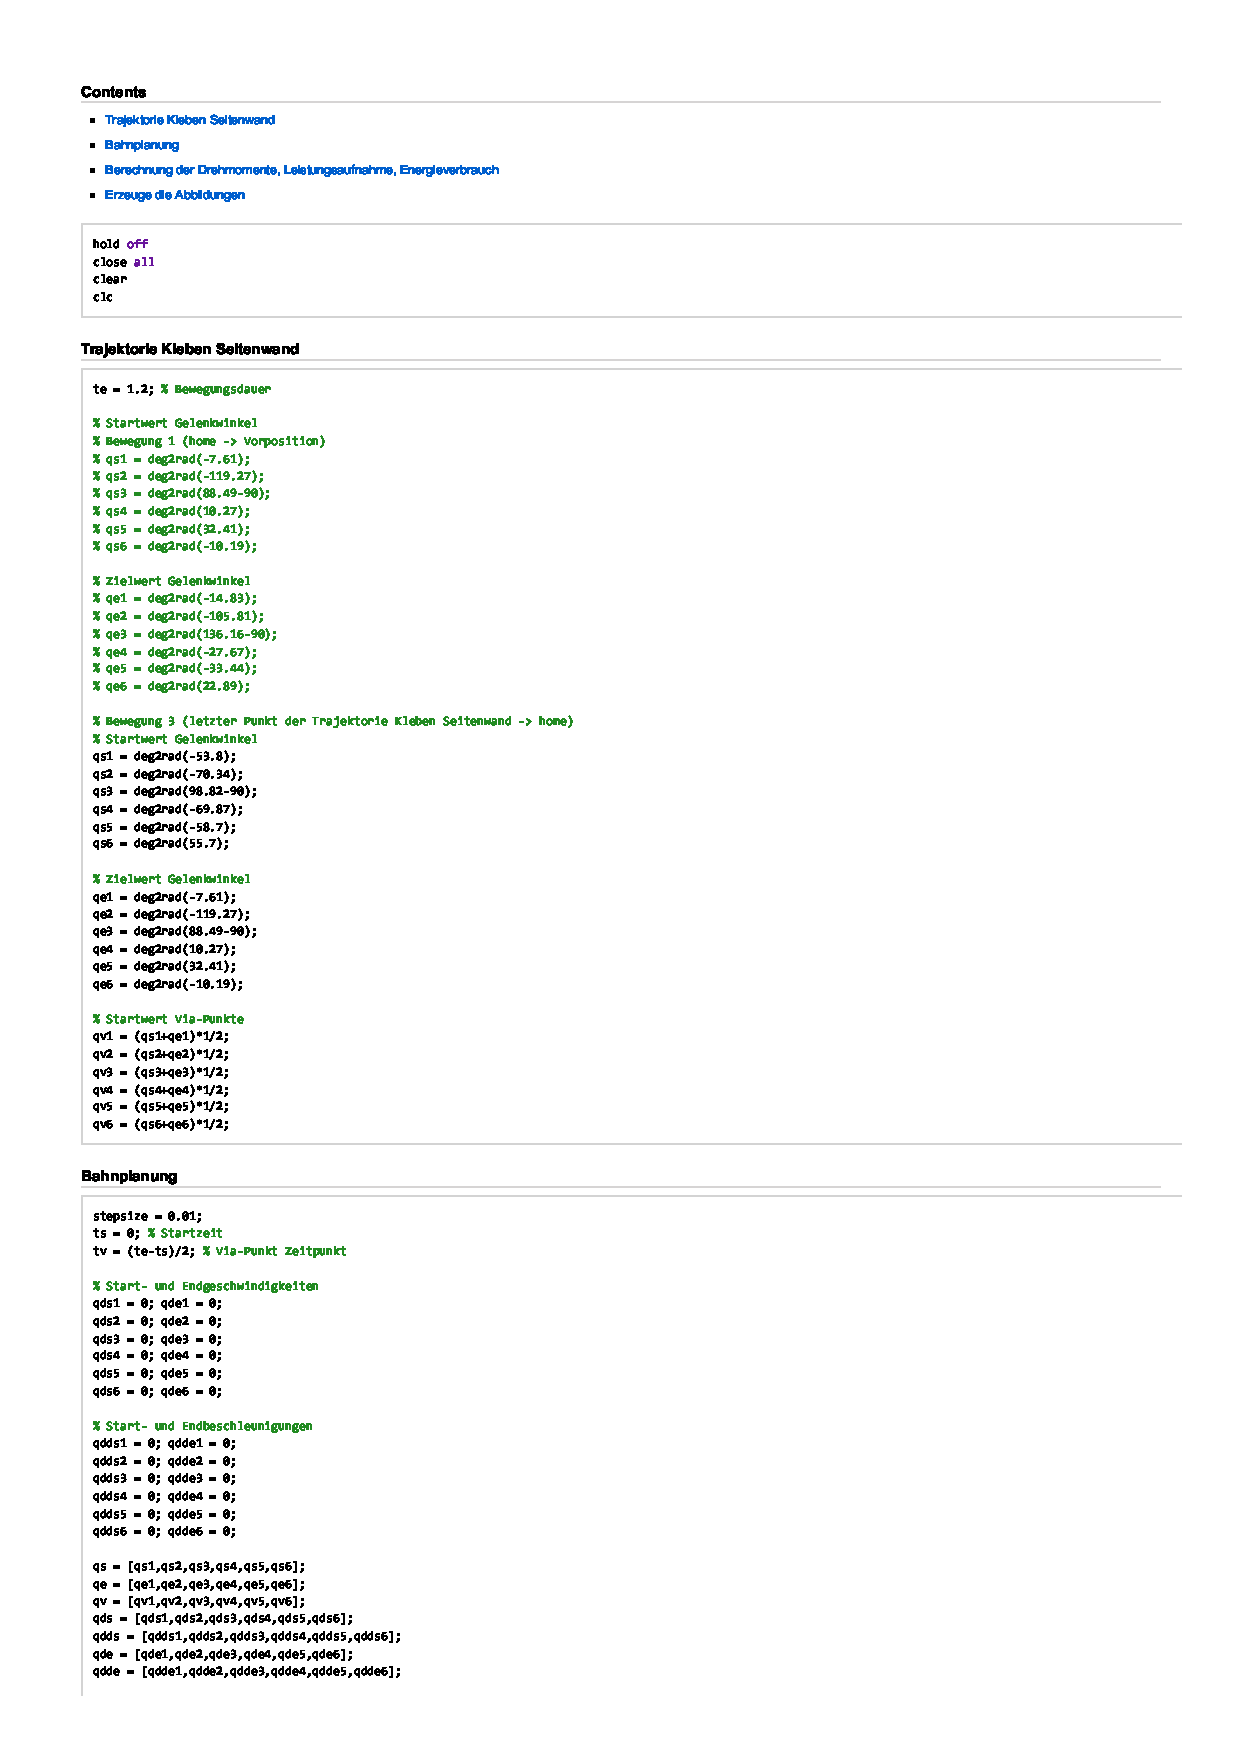
\includepdf[pages=1-2]{C:/Users/denni/Documents/Bachelorarbeit/BachelorThesis/literature/Anhang/simulation_matlab.pdf}
\subsection*{Funktionalitäten}
%
\begin{itemize}
	\setlength{\itemsep}{-1ex}
	\item Trajektorie Kleben Seitenwand
	\item Bewegung 1 (home -\ensuremath{>} Vorposition)
	\item Bewegung 3 (letzter Punkt der Trajektorie Kleben Seitenwand -\ensuremath{>} home)
	\item Bahnplanung
	\item Modellberechnung der Drehmomente, Leistungsaufnahme
	\item Daten Vorverarbeitung
	\item Anzeige der Daten
	\item Erzeuge die Abbildungen
\end{itemize}
\begin{lstlisting}
	hold off
	close all
	clear
	clc
\end{lstlisting}
%
\subsection*{Trajektorie Kleben Seitenwand}
%
\begin{lstlisting}
	te = 1.2; % Bewegungsdauer
\end{lstlisting}
%
\subsection*{Bewegung 1 (home -\ensuremath{>} Vorposition)}
%
\begin{par}
	\% Startwert Gelenkwinkel qs1 = deg2rad(-7.61); qs2 = deg2rad(-119.27); qs3 = deg2rad(88.49-90); qs4 = deg2rad(10.27); qs5 = deg2rad(32.41); qs6 = deg2rad(-10.19);
\end{par} \vspace{1em}
\begin{par}
	\% Zielwert Gelenkwinkel qe1 = deg2rad(-14.83); qe2 = deg2rad(-105.81); qe3 = deg2rad(136.16-90); qe4 = deg2rad(-27.67); qe5 = deg2rad(-33.44); qe6 = deg2rad(22.89);
\end{par} \vspace{1em}
\begin{lstlisting}
	% optimierte Via-Punkte
	% qvd = [];
	% qv1 = deg2rad(qvd(1));
	% qv2 = deg2rad(qvd(2));
	% qv3 = deg2rad(qvd(3));
	% qv4 = deg2rad(qvd(4));
	% qv5 = (deg2rad(qvd(5))+(qs5+qe5)*1/2)*1/2; % Für den Fall, dass der Wert zu dicht an den Grenzen liegt, was eine hohe Beschleunigung zur Folge hat, wird das Mittel aus dem optimierten und dem initialen Via-Punkt gebildet
	% qv6 = (deg2rad(qvd(6))+(qs6+qe6)*1/2)*1/2;
\end{lstlisting}
%
\subsection*{Bewegung 3 (letzter Punkt der Trajektorie Kleben Seitenwand -\ensuremath{>} home)}
%
\begin{par}
	Startwert Gelenkwinkel
\end{par} \vspace{1em}
\begin{lstlisting}
	qs1 = deg2rad(-53.8);
	qs2 = deg2rad(-70.34);
	qs3 = deg2rad(98.82-90);
	qs4 = deg2rad(-69.87);
	qs5 = deg2rad(-58.7);
	qs6 = deg2rad(55.7);
	
	% Zielwert Gelenkwinkel
	qe1 = deg2rad(-7.61);
	qe2 = deg2rad(-119.27);
	qe3 = deg2rad(88.49-90);
	qe4 = deg2rad(10.27);
	qe5 = deg2rad(32.41);
	qe6 = deg2rad(-10.19);
	
	% % Startwert Via-Punkte
	% qv1 = (qs1+qe1)*1/2;
	% qv2 = (qs2+qe2)*1/2;
	% qv3 = (qs3+qe3)*1/2;
	% qv4 = (qs4+qe4)*1/2;
	% qv5 = (qs5+qe5)*1/2;
	% qv6 = (qs6+qe6)*1/2;
	
	% optimierte Via-Punkte
	qvu = [-25.0007 -96.0711 8.8200 10.2700 -47.7822 -10.1900];
	qv1 = deg2rad(qvu(1));
	qv2 = deg2rad(qvu(2));
	qv3 = deg2rad(qvu(3));
	qv4 = (deg2rad(qvu(4))+(qs4+qe4)*1/2)*1/2;
	qv5 = (deg2rad(qvu(5))+(qs5+qe5)*1/2)*1/2;
	qv6 = (deg2rad(qvu(6))+(qs6+qe6)*1/2)*1/2;
\end{lstlisting}
%
\subsection*{Bahnplanung}
%
\begin{lstlisting}
	stepsize = 0.004;
	ts = 0; % Startzeit
	tv = (te-ts)/2; % Via-Punkt Zeitpunkt
	
	% Start- und Endgeschwindigkeiten
	qds1 = 0; qde1 = 0;
	qds2 = 0; qde2 = 0;
	qds3 = 0; qde3 = 0;
	qds4 = 0; qde4 = 0;
	qds5 = 0; qde5 = 0;
	qds6 = 0; qde6 = 0;
	
	% Start- und Endbeschleunigungen
	qdds1 = 0; qdde1 = 0;
	qdds2 = 0; qdde2 = 0;
	qdds3 = 0; qdde3 = 0;
	qdds4 = 0; qdde4 = 0;
	qdds5 = 0; qdde5 = 0;
	qdds6 = 0; qdde6 = 0;
	
	qs = [qs1,qs2,qs3,qs4,qs5,qs6];
	qe = [qe1,qe2,qe3,qe4,qe5,qe6];
	qv = [qv1,qv2,qv3,qv4,qv5,qv6];
	qds = [qds1,qds2,qds3,qds4,qds5,qds6];
	qdds = [qdds1,qdds2,qdds3,qdds4,qdds5,qdds6];
	qde = [qde1,qde2,qde3,qde4,qde5,qde6];
	qdde = [qdde1,qdde2,qdde3,qdde4,qdde5,qdde6];
	
	% Bahnplanung Polynom 6-Ordnung
	[q1,qd1,qdd1,~] = trajectorie_planning_sixth_order(ts, te, tv, stepsize, qs(1), qds(1), qdds(1), qv(1), qe(1), qde(1), qdde(1));
	[q2,qd2,qdd2,~] = trajectorie_planning_sixth_order(ts, te, tv, stepsize, qs(2), qds(2), qdds(2), qv(2), qe(2), qde(2), qdde(2));
	[q3,qd3,qdd3,~] = trajectorie_planning_sixth_order(ts, te, tv, stepsize, qs(3), qds(3), qdds(3), qv(3), qe(3), qde(3), qdde(3));
	[q4,qd4,qdd4,~] = trajectorie_planning_sixth_order(ts, te, tv, stepsize, qs(4), qds(4), qdds(4), qv(4), qe(4), qde(4), qdde(4));
	[q5,qd5,qdd5,~] = trajectorie_planning_sixth_order(ts, te, tv, stepsize, qs(5), qds(5), qdds(5), qv(5), qe(5), qde(5), qdde(5));
	[q6,qd6,qdd6,t] = trajectorie_planning_sixth_order(ts, te, tv, stepsize, qs(6), qds(6), qdds(6), qv(6), qe(6), qde(6), qdde(6));
\end{lstlisting}
%
\subsection*{Modellberechnung der Drehmomente, Leistungsaufnahme}
%
\begin{lstlisting}
	% Initialisierung
	tau = zeros(length(t));
	Pmech = zeros(length(t));
	Pmech_diss = zeros(length(t));
	Pmech_sink = zeros(length(t));
	
	% RNEA
	for index = 1:1:(length(t))
	[ret_tau,ret_Pmech] = rnea(q1(index), q2(index), q3(index), q4(index), q5(index), q6(index), qd1(index), qd2(index), qd3(index), qd4(index), qd5(index), qd6(index), qdd1(index), qdd2(index), qdd3(index), qdd4(index), qdd5(index), qdd6(index));
	tau(index,1) = ret_tau(1);
	tau(index,2) = ret_tau(2);
	tau(index,3) = ret_tau(3);
	tau(index,4) = ret_tau(4);
	tau(index,5) = ret_tau(5);
	tau(index,6) = ret_tau(6);
	Pmech(index,1) = ret_Pmech(1);
	Pmech(index,2) = ret_Pmech(2);
	Pmech(index,3) = ret_Pmech(3);
	Pmech(index,4) = ret_Pmech(4);
	Pmech(index,5) = ret_Pmech(5);
	Pmech(index,6) = ret_Pmech(6);
	end
\end{lstlisting}
%
\subsection*{Daten Vorverarbeitung}
%
\begin{lstlisting}
	for index = 1:1:(length(t))
	for var = 1:6
	if Pmech(index,var) > 0
	Pmech_sink(index,var) = Pmech(index,var);
	else
	Pmech_diss(index,var) = Pmech(index,var);
	Pmech_sink(index,var) = 0;
	
	end
	end
	end
\end{lstlisting}
%
\subsection*{Anzeige der Daten}
%
\begin{lstlisting}
	disp('qv1');disp(rad2deg(qv1));
	disp('qv2');disp(rad2deg(qv2));
	disp('qv3');disp(rad2deg(qv3));
	disp('qv4');disp(rad2deg(qv4));
	disp('qv5');disp(rad2deg(qv5));
	disp('qv6');disp(rad2deg(qv6));
	torque = sum(sum(abs(tau)))/length(t); disp('Mittelwert der Summe des Betrags der Getriebe-Drehmomente in Nm'); disp(torque);
	P_mech = sum(sum((Pmech_sink))/length(t)); disp('Mittelwert der aufgenommenen mechanischen Leistung in W'); disp(P_mech);
	P_mech_diss = sum(sum((Pmech_diss))/length(t))*(te-ts); disp('Dissipierte Energie in J'); disp(P_mech_diss);
	E_mech = sum(sum(Pmech_sink)/length(t))*(te-ts); disp('Aufgenommene Energie in J'); disp(E_mech);
\end{lstlisting}
%
\subsection*{Erzeuge die Abbildungen}
%
\begin{lstlisting}
	show_graphics(q1, q2, q3, q4, q5, q6, qd1, qd2, qd3, qd4, qd5, qd6, qdd1, qdd2, qdd3, qdd4, qdd5, qdd6, t, tau, Pmech)
\end{lstlisting}
%
%
\section{Berechnung der Zielfunktion}
%
\label{add:zielfunktion}
\subsection*{Funktionalitäten}
%
\begin{itemize}
	\setlength{\itemsep}{-1ex}
	\item Bahnplanung
	\item jacobi
	\item Modellberechnung der Drehmomente, Leistungsaufnahme
	\item Daten Vorverarbeitung
	\item Anzeige der Daten
\end{itemize}
\begin{lstlisting}
	function [E_mech] = calc_objective(qs,qe,qv,te)
\end{lstlisting}
\begin{lstlisting}
	% Berechung der Zielfunktion (Energieverbrauch) über die nicht
	% dissipierte mechanische Leistung
\end{lstlisting}
%
\subsection*{Bahnplanung}
%
\begin{lstlisting}
	stepsize = 0.004;
	ts = 0;
	tv = (te-ts)/2;
	
	qds1 = 0; qde1 = 0;
	qds2 = 0; qde2 = 0;
	qds3 = 0; qde3 = 0;
	qds4 = 0; qde4 = 0;
	qds5 = 0; qde5 = 0;
	qds6 = 0; qde6 = 0;
	
	qdds1 = 0; qdde1 = 0;
	qdds2 = 0; qdde2 = 0;
	qdds3 = 0; qdde3 = 0;
	qdds4 = 0; qdde4 = 0;
	qdds5 = 0; qdde5 = 0;
	qdds6 = 0; qdde6 = 0;
	
	qds = [qds1,qds2,qds3,qds4,qds5,qds6];
	qdds = [qdds1,qdds2,qdds3,qdds4,qdds5,qdds6];
	qde = [qde1,qde2,qde3,qde4,qde5,qde6];
	qdde = [qdde1,qdde2,qdde3,qdde4,qdde5,qdde6];
	
	[q1,qd1,qdd1,~] = trajectorie_planning_sixth_order(ts, te, tv, stepsize, qs(1), qds(1), qdds(1), qv(1), qe(1), qde(1), qdde(1));
	[q2,qd2,qdd2,~] = trajectorie_planning_sixth_order(ts, te, tv, stepsize, qs(2), qds(2), qdds(2), qv(2), qe(2), qde(2), qdde(2));
	[q3,qd3,qdd3,~] = trajectorie_planning_sixth_order(ts, te, tv, stepsize, qs(3), qds(3), qdds(3), qv(3), qe(3), qde(3), qdde(3));
	[q4,qd4,qdd4,~] = trajectorie_planning_sixth_order(ts, te, tv, stepsize, qs(4), qds(4), qdds(4), qv(4), qe(4), qde(4), qdde(4));
	[q5,qd5,qdd5,~] = trajectorie_planning_sixth_order(ts, te, tv, stepsize, qs(5), qds(5), qdds(5), qv(5), qe(5), qde(5), qdde(5));
	[q6,qd6,qdd6,t] = trajectorie_planning_sixth_order(ts, te, tv, stepsize, qs(6), qds(6), qdds(6), qv(6), qe(6), qde(6), qdde(6));
\end{lstlisting}
%
\subsection*{Modellberechnung der Drehmomente, Leistungsaufnahme}
%
\begin{lstlisting}
	% Initialisierung
	tau = zeros(length(t));
	Pmech = zeros(length(t));
	Pmech_diss = zeros(length(t));
	Pmech_sink = zeros(length(t));
	
	for index = 1:1:(length(t))
	[ret_tau,ret_Pmech] = rnea(q1(index), q2(index), q3(index), q4(index), q5(index), q6(index), qd1(index), qd2(index), qd3(index), qd4(index), qd5(index), qd6(index), qdd1(index), qdd2(index), qdd3(index), qdd4(index), qdd5(index), qdd6(index));
	tau(index,1) = ret_tau(1);
	tau(index,2) = ret_tau(2);
	tau(index,3) = ret_tau(3);
	tau(index,4) = ret_tau(4);
	tau(index,5) = ret_tau(5);
	tau(index,6) = ret_tau(6);
	Pmech(index,1) = ret_Pmech(1);
	Pmech(index,2) = ret_Pmech(2);
	Pmech(index,3) = ret_Pmech(3);
	Pmech(index,4) = ret_Pmech(4);
	Pmech(index,5) = ret_Pmech(5);
	Pmech(index,6) = ret_Pmech(6);
	end
\end{lstlisting}
%
\subsection*{Daten Vorverarbeitung}
%
\begin{lstlisting}
	for index = 1:1:(length(t))
	for var = 1:6
	if Pmech(index,var) > 0
	Pmech_sink(index,var) = Pmech(index,var);
	else
	Pmech_diss(index,var) = Pmech(index,var);
	Pmech_sink(index,var) = 0;
	end
	end
	end
\end{lstlisting}
%
\subsection*{Anzeige der Daten}
%
\begin{lstlisting}
	torque = sum(sum((tau).^2))/length(t);
	E_mech = sum(sum((Pmech_sink))/length(t))*(te-ts); disp('E in J'); disp(E_mech);
\end{lstlisting}
\begin{lstlisting}
	end
\end{lstlisting}
%
%
\section{Optimierung}
\label{acc:optimierer}
%
\subsection*{Funktionalitäten}
%
\begin{itemize}
	\setlength{\itemsep}{-1ex}
	\item KlebenSeitenwand
	\item Bewegung 1 (home -\ensuremath{>} Vorposition)
	\item Bewegung 3 (letzter Punkt der Trajektorie Kleben Seitenwand -\ensuremath{>} home)
	\item Startwert Via-Punkte
	\item Initial-Trajektorie-Definition
	\item Definition Optimierer
\end{itemize}
\begin{lstlisting}
	hold off
	close all
	clear
	clc
\end{lstlisting}
%
\subsection*{KlebenSeitenwand}
%
\subsection*{Bewegung 1 (home -\ensuremath{>} Vorposition)}
%
\begin{par}
	\% Startwert Gelenkwinkel qs1 = deg2rad(-7.61); qs2 = deg2rad(-119.27); qs3 = deg2rad(88.49-90); qs4 = deg2rad(10.27); qs5 = deg2rad(32.41); qs6 = deg2rad(-10.19);
\end{par} \vspace{1em}
\begin{par}
	\% Zielwert Gelenkwinkel qe1 = deg2rad(-14.83); qe2 = deg2rad(-105.81); qe3 = deg2rad(136.16-90); qe4 = deg2rad(-27.67); qe5 = deg2rad(-33.44); qe6 = deg2rad(22.89);
\end{par} \vspace{1em}
%
\subsection*{Bewegung 3 (letzter Punkt der Trajektorie Kleben Seitenwand -\ensuremath{>} home)}
%
\begin{par}
	Startwert Gelenkwinkel
\end{par} \vspace{1em}
\begin{lstlisting}
	qs1 = deg2rad(-53.8);
	qs2 = deg2rad(-70.34);
	qs3 = deg2rad(98.82-90);
	qs4 = deg2rad(-69.87);
	qs5 = deg2rad(-58.7);
	qs6 = deg2rad(55.7);
	
	% Zielwert Gelenkwinkel
	qe1 = deg2rad(-7.61);
	qe2 = deg2rad(-119.27);
	qe3 = deg2rad(88.49-90);
	qe4 = deg2rad(10.27);
	qe5 = deg2rad(32.41);
	qe6 = deg2rad(-10.19);
\end{lstlisting}
%
\subsection*{Startwert Via-Punkte}
%
\begin{lstlisting}
	denum = 1; % Testen von Startwerten, die von Mittelpunkt abweichen
	qv1 = (qs1+qe1)*1/2;%-(abs(qs1-qe1)/2)/denum;
	qv2 = (qs2+qe2)*1/2;%-(abs(qs1-qe1)/2)/denum;
	qv3 = (qs3+qe3)*1/2;%-(abs(qs1-qe1)/2)/denum;
	qv4 = (qs4+qe4)*1/2;%-(abs(qs1-qe1)/2)/denum;
	qv5 = (qs5+qe5)*1/2;%-(abs(qs1-qe1)/2)/denum;
	qv6 = (qs6+qe6)*1/2;%-(abs(qs1-qe1)/2)/denum;
\end{lstlisting}
%
\subsection*{Initial-Trajektorie-Definition}
%
\begin{lstlisting}
	te = 1.2;
	qs = [qs1,qs2,qs3,qs4,qs5,qs6];
	qe = [qe1,qe2,qe3,qe4,qe5,qe6];
	qv = [qv1,qv2,qv3,qv4,qv5,qv6];
\end{lstlisting}
%
\subsection*{Definition Optimierer}
%
\begin{par}
	Zielfunktion
\end{par} \vspace{1em}
\begin{lstlisting}
	objective = @(qv) calc_objective(qs,qe,qv,te);
	% Startwert
	x0 = qv;
	% Anzeige des Energieverbrauchs beim Start der Optimierung
	disp(['initial Objective: ' num2str(objective(x0))]);
	% Gleichheitsnebenbedingungen
	A = [];
	b = [];
	% Ungleichheitsnebenbedingungen
	Aeq = [];
	beq = [];
	% Grenzen des Parametervektors
	lb = (qv-(abs(qs-qe))/2);
	ub = (qv+(abs(qs-qe))/2);
	% Nichtlineare Nebenbedingungen
	nonlcon = [];
	% Auswahl des Solvers fmincon
	% Algorithmus sequentielle quadratische Programmierung
	% max. Anzahl der Iterationen = 25
	% und Ausgabe des Zielfunktionswertes mit jeder Iteration
	options = optimoptions(@fmincon,'Algorithm','sqp', 'MaxIterations', 25,'PlotFcn',@optimplotfval);
	% Ausführen der Optimierung
	[x,fval,ef,output,lambda] = fmincon(objective,x0,A,b,Aeq,beq,lb,ub,nonlcon,options);
	% Anzeige des energieoptimalen Parametervektors
	disp(x*180/pi)
\end{lstlisting}
\color{lightgray} \begin{lstlisting}
% Startwert
E in J
2.0013e+03

% Zielwert
E in J
1.8074e+03

% identifzierter Parametervektor
-24.8857 -96.0716 8.8200 10.2700 -47.5666 -10.1900

\end{lstlisting} \color{black}
%
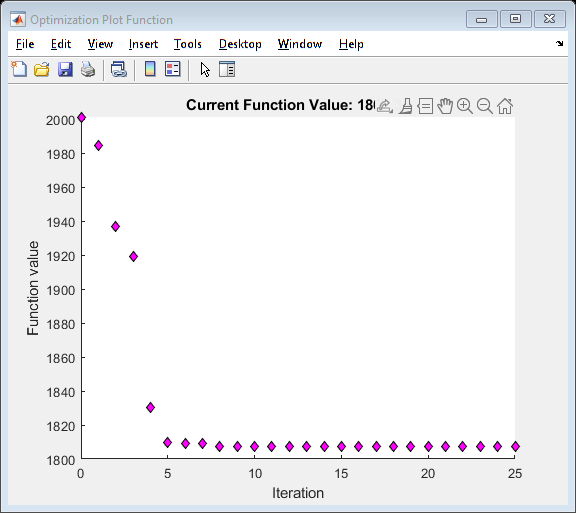
\includegraphics [width=4in]{images/optimization_01}
%
\section{Vergleich der simulierten Verläufe für den initialen und justierten, energieoptimalen Parametervektor}
\label{acc:optupjust}
%
in Abbildung \ref{fig:posoptfinal} wird ersichtlich, dass die Gelenkwinkel $q_{i,justiert}(t)$ innerhalb der Start- und Zielwinkel liegen.
%
\begin{equation}
	q_{i,justiert}(t) \in [q_{i,s};q_{i,e}] ~\forall~ i \in \{1,2,3,4,5,6\}
\end{equation}
%
Die erreichten Winkelgeschwindigkeiten liegen unterhalb der in \ref{add:datenblatt} notierten Winkelgeschwindigkeiten bei Nenn-Traglast.
%
\begin{figure}[tbph]
	\centering
	\includegraphics[width=1\linewidth]{images/Optimierungsergebnisse_up/posoptfinal}
	\caption{Gelenkwinkelverläufe der Initialbahn und justierten energieoptimierten Bewegungsbahn}
	\label{fig:posoptfinal}
\end{figure}
%
\begin{figure}[tbph]
	\centering
	\includegraphics[width=1\linewidth]{images/Optimierungsergebnisse_up/veloptfinal}
	\caption{Winkelgeschwindigkeitsverläufe der Initialbahn und justierten energieoptimierten Bewegungsbahn}
	\label{fig:veloptfinal}
\end{figure}
%
\begin{figure}[tbph]
	\centering
	\includegraphics[width=1\linewidth]{images/Optimierungsergebnisse_up/accoptfinal}
	\caption{Winkelbeschleunigungsverläufe der Initialbahn und justierten energieoptimierten Bewegungsbahn}
	\label{fig:accoptfinal}
\end{figure}
%
Der qualitative Verlauf der aufgenommenen Leistung für den justierten energieoptimalen Parametervektor entspricht dem des energieoptimalen Parametervektors. 
%
\begin{figure}[tbph]
	\centering
	\includegraphics[width=1\linewidth]{images/Optimierungsergebnisse_up/tauoptfinal}
	\caption{Drehmomentverläufe der Initialbahn und justierten energieoptimierten Bewegungsbahn}
	\label{fig:tauoptfinal}
\end{figure}
%
\begin{figure}[tbph]
	\centering
	\includegraphics[width=1\linewidth]{images/Optimierungsergebnisse_up/poptfinal}
	\caption{Verläufe der aufgenommen Leistung je Gelenkwinkel für die Initialbahn und justierte energieoptimierte Bewegungsbahn}
	\label{fig:poptfinal}
\end{figure}

%%\addchap{Anhang E}
%\setcounter{chapter}{5}
%\setcounter{section}{0}
%\setcounter{table}{0}
%\setcounter{figure}{0}
%
%\section{Wichtige \LaTeX -Befehle}
%
%\begin{tabbing}
%\hspace*{0cm} \= \hspace{0.28\linewidth} \= \+\kill
%\textbackslash \textit{label}\{\}	\> Definition eines Labels, auf welches referenziert werden kann\\ 
%	\> z.B.: \textbackslash \textit{label}\{fig:MyImage\}\\ 
%\textbackslash \textit{ref}\{\}	\> Setzen einer Referenz zu einem Label\\
%\textbackslash \textit{pageref}\{\}	\> Gibt die Seitenzahl zu einer Referenz zurück\\
%	\> z.B.: Tabelle\~{}\textbackslash \textit{ref}\{tab:messdaten\} fasst die Messergebnisse zusammen.\\ 
%\textbackslash \textit{cite}\{\}	\> Literaturreferenz einfügen\\
%\textbackslash \textit{cite}[S. x]\{\}	\> Literaturreferenz mit Angabe einer Seitenzahl \glqq x\grqq~einfügen\\
%
%\textbackslash \textit{footnote}\{\}	\> Fußnote einfügen\\ 
%\~{}	\> Einfügen eines geschützten Leerzeichens\\ 
%\textdollar \textit{Formel} \textdollar	\> Eingabe einer Formel im Text\\
%\textbackslash \textit{nomenclature}\{a.\}\{ab\}	\> Aufnahme der Abkürzung \glqq a.\grqq~für \glqq ab\grqq~in das Abkürzungsverzeichnis.\\
%\textbackslash \textit{index}\{Obst!Birne\} \> Aufnahme des Begriffs \glqq Birne\grqq~in den Index unter \glqq Obst\grqq. \index{Obst!Birne} \\
%\textbackslash \textit{clearpage}	\> Ausgabe aller Gleitobjekte und Umbruch auf neue Seite\\ 
%\end{tabbing}
%
%\clearpage
%
%\section{Vorlagen für \LaTeX Umgebungen}
%
%\subsection{Listen und Aufzählungen}
%
%Es gibt folgende Listentypen. Die wichtigsten:
%
%\begin{itemize}
%	\item Einfache Liste mit \textit{itemize}-Umgebung
%	\item ...
%\end{itemize}
%
%\begin{enumerate}
%	\item Nummerierte Liste mit \textit{enumerate}-Umgebung
%	\item ...
%\end{enumerate}
%
%\begin{enumerate}[label=\alph*.]
%	\item wobei man bei der \textit{enumerate}-Umgebung leicht die Art der Nummerierung ändern kann,
%	\item ...
%\end{enumerate}
%
%und durch verschachtelte Umgebungen verschiedene Aufzählungsebenen darstellen kann:
%
%\begin{enumerate}[label=\alph*)]
%	\item Erster Aufzählungspunkt der ersten Ebene
%	\item ...
%	\begin{itemize}
%		\item Erster Punkt der zweiten Ebene
%		\item Zweiter Punkt der zweiten Ebene
%	\end{itemize}
%	\item Das sollte an Beispielen zunächst einmal genügen.
%\end{enumerate}
%
%\clearpage
%
%\subsection{Bilder und Grafiken}
%
%Bilder können als PDF-, JPG-, und PNG-Bilder in \LaTeX eingebunden werden. Damit eine Grafik in hoher Qualität dargestellt wird, sollte das Dateiformat der Grafik vektorbasiert sein, d.h. als PDF-Datei vorliegen. Viele Zeichenprogramme unterstützen einen PDF-Export (z.B. GIMP, Adobe Illustrator, etc.). Für Grafiken aus PowerPoint sei folgende Vorgehensweise beim Export empfohlen:
%
%\begin{enumerate}
%	\item Die gewünschte Grafik in PowerPoint zeichnen.
%	\item Gewünschten Bildbereich markieren, rechte Maustaste klicken und \glqq Als Grafik speichern ...\grqq~wählen.
%	\item Grafik im Format EMF abspeichern. Das EMF-Format ist vektorbasiert.\footnote{Mit dem Mac kann in PowerPoint die Grafik direkt im PDF-Format exportiert werden. Die weiteren Schritte entfallen daher.}
%	\item Mit dem Programm XnView die Grafik im EMF-Format in PDF wandeln und abspeichern.
%	\item Die so erzeugte PDF-Datei enthält eine vektorbasierte Grafik und kann in \LaTeX~ eingebunden werden.
%\end{enumerate}
%
%Abbildung~\ref{fig:MyImage} zeigt ein Beispielbild einer Grafik, welche aus PowerPoint exportiert wurde.
%
%\begin{figure}[hbt]
%	\centering
%	\includegraphics[width=0.3\linewidth]{images/MyImage}
%	\caption[Beispiel für die Einbindung eines Bildes.]{Beispiel für die Einbindung eines Bildes (PDF-, JPG-, und PNG-Bilder können eingebunden werden).}
%	\label{fig:MyImage}
%\end{figure}
%
%Der Quellcode des Beispielbildes aus Abbildung~\ref{fig:MyImage} ist in Listing~\ref{lst:fig} zu sehen.
%
%\clearpage
%
%\begin{lstlisting}[caption=Quellcode der Abbildung~\ref{fig:MyImage}.,label=lst:fig]
%\begin{figure}[hbt]				% here, bottom, top
%\centering						% Zentrierung
%\includegraphics[width=0.6\linewidth]{images/MyImage}		
%\caption[Beispiel für die Einbindung eines Bildes.]{Beispiel für die Einbindung eines Bildes (PDF-, JPG-, und PNG-Bilder können eingebunden werden).}
%\label{fig:MyImage}
%\end{figure}
%\end{lstlisting}
%
%Grafiken können auch mithilfe des Packages Tikz gezeichnet, bzw. programmiert werden. Grafiken mit Tikz werden mit dem \textit{input}-Befehl in die \textit{figure}-Umgebung geladen, wie nachfolgendes Beispiel in Abbildung~\ref{fig:tikz_house} zeigt:
%
%\begin{figure}[hbt]
%	\centering
%	 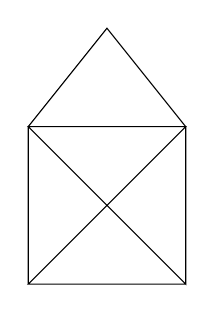
\begin{tikzpicture}
\draw (0,0) -- (0,2) -- (1,3.25) -- (2,2) -- (2,0) -- (0,2) -- (2,2) -- (0,0) -- (2,0);
\end{tikzpicture}
    
%	\caption[Mit Tikz programmierte Grafik.]{Mit Tikz programmierte Grafik.}
%	\label{fig:tikz_house}
%\end{figure}
%
%Ein etwas umfangreicheres Beispiel zur Digitaltechnik ist in Abbildung~\ref{fig:tikz_digital} dargestellt:
%
%\begin{figure}[hbt]
%	\centering
%	\usetikzlibrary{circuits.logic.US,circuits.logic.IEC}
      \begin{tikzpicture}[circuit logic US]
      \matrix[column sep=7mm]
      {
      \node (i0) {0}; & & \\
      & \node [and gate] (a1) {}; & \\
      \node (i1) {0}; & & \node [or gate] (o) {};\\
      & \node [nand gate] (a2) {}; & \\
      \node (i2) {1}; & & \\
      };
      \draw (i0.east) -- ++(right:3mm) |- (a1.input 1);
      \draw (i1.east) -- ++(right:3mm) |- (a1.input 2);
      \draw (i1.east) -- ++(right:3mm) |- (a2.input 1);
      \draw (i2.east) -- ++(right:3mm) |- (a2.input 2);
      \draw (a1.output) -- ++(right:3mm) |- (o.input 1);
      \draw (a2.output) -- ++(right:3mm) |- (o.input 2);
      \draw (o.output) -- ++(right:3mm) node [right] {$y$ \quad Hier könnte Ihre Formel $y=(0 \land 0) \lor \overline{( 0 \land 1)}$ stehen};
 \end{tikzpicture}

%	\caption[Mit Tikz programmierte Grafik, welche bereits vorgefertigte Bibliotheken für Symbole aus der Digitaltechnik nutzt.]{Mit Tikz programmierte Grafik, welche bereits vorgefertigte Bibliotheken für Symbole aus der Digitaltechnik nutzt.}
%	\label{fig:tikz_digital}
%\end{figure}
%
%\clearpage
%
%In der Tikz-Umgebung können auch Diagramme mit dem \textit{pgfplot}-Befehlssatz erzeugt werden. In Abbildung \ref{fig:pgfplot} sehen Sie ein Beispiel.
%
%\begin{figure}[hbt]
%	\centering
%	\begin{tikzpicture}
		\begin{axis}[scale=1.3,legend entries={Messwerte mit Fehlerbalken,
			$\pgfmathprintnumber{\pgfplotstableregressiona} \cdot x  
			\pgfmathprintnumber[print sign]{\pgfplotstableregressionb}$}, legend style={draw=none},legend style={at={(0.01,0.98)},anchor=north west},xlabel=Stromstärke $I \; \mathrm{ \lbrack mA \rbrack}$,ylabel=Spannung $U \; \mathrm{ \lbrack V \rbrack}$]
		\addlegendimage{mark=*,blue}
		\addlegendimage{no markers,red}
\addplot+[error bars/.cd, y dir=both,y explicit]
table[x=x,y=y,y error=errory] 
{pgfplot/messdaten_mitfehler.dat};
\addplot table[mark=none,y={create col/linear regression={y=y}}]
{pgfplot/messdaten_mitfehler.dat};
	\end{axis}
\end{tikzpicture}
%	\caption[Diagramm, erstellt mit dem \textit{pgfplot}-Befehlssatz.]{Ein Diagramm, erstellt in der \textit{tikzpicture}-Umgebung mit dem \textit{pgfplot}-Befehlssatz. Das Diagramm stellt Messdaten, deren Fehlerbalken und eine Regressionskurve dar. Die Messdaten werden von einer separaten Datei eingelesen und die Regressionskurve wurde mit \textit{pgfplot} berechnet und erstellt.}
%	\label{fig:pgfplot}
%\end{figure}
%
%\clearpage
%
%Auch hierzu der Quellcode in Listing~\ref{lst:pgfplot}.
%
%\begin{lstlisting}[caption=Quellcode der Abbildung~\ref{fig:pgfplot}.,label=lst:pgfplot]
%\begin{figure}[hbt]
%\centering
%\begin{tikzpicture}
		\begin{axis}[scale=1.3,legend entries={Messwerte mit Fehlerbalken,
			$\pgfmathprintnumber{\pgfplotstableregressiona} \cdot x  
			\pgfmathprintnumber[print sign]{\pgfplotstableregressionb}$}, legend style={draw=none},legend style={at={(0.01,0.98)},anchor=north west},xlabel=Stromstärke $I \; \mathrm{ \lbrack mA \rbrack}$,ylabel=Spannung $U \; \mathrm{ \lbrack V \rbrack}$]
		\addlegendimage{mark=*,blue}
		\addlegendimage{no markers,red}
\addplot+[error bars/.cd, y dir=both,y explicit]
table[x=x,y=y,y error=errory] 
{pgfplot/messdaten_mitfehler.dat};
\addplot table[mark=none,y={create col/linear regression={y=y}}]
{pgfplot/messdaten_mitfehler.dat};
	\end{axis}
\end{tikzpicture}
%\caption[Diagramm, erstellt mit dem \textit{pgfplot}-Befehlssatz.]{Ein Diagramm, erstellt in der \textit{tikzpicture}-Umgebung mit dem \textit{pgfplot}-Befehlssatz. Das Diagramm stellt Messdaten, deren Fehlerbalken und eine Regressionskurve dar. Die Messdaten werden von einer separaten Datei eingelesen und die Regressionskurve wurde mit \textit{pgfplot} berechnet und erstellt.}
%\label{fig:pgfplot}
%\end{figure}
%\end{lstlisting}
%
%In Listing~\ref{lst:tikz} ist der Quellcode der Datei \textit{mess\_fehlerbalken.tex} dargestellt.
%
%\begin{lstlisting}[caption=Quellcode der Datei \textit{mess\_fehlerbalken.tex}.,label=lst:tikz]
%\begin{tikzpicture}
%\begin{axis}[scale=1.3,legend entries={Messwerte mit Fehlerbalken,
%$\pgfmathprintnumber{\pgfplotstableregressiona} \cdot x  
%\pgfmathprintnumber[print sign]{\pgfplotstableregressionb}$}, legend style={draw=none},legend style={at={(0.01,0.98)},anchor=north west},xlabel=Stromstärke $I \; \mathrm{ \lbrack mA \rbrack}$,ylabel=Spannung $U \; \mathrm{ \lbrack V \rbrack}$]
%\addlegendimage{mark=*,blue}
%\addlegendimage{no markers,red}
%\addplot+[error bars/.cd, y dir=both,y explicit]
%table[x=x,y=y,y error=errory] 
%{pgfplot/messdaten_mitfehler.dat};
%\addplot table[mark=none,y={create col/linear regression={y=y}}]
%{pgfplot/messdaten_mitfehler.dat};
%\end{axis}
%\end{tikzpicture}
%\end{lstlisting}
%
%\clearpage
%
%In Abbildung~\ref{fig:pgfplot2y} wird ein weiters Beispiel für ein Diagramm gezeigt. Oftmals wird eine zweite y-Achse verwendet, um verschiedene Skalen darstellen zu können.
%
%\begin{figure}[hbt]
%	\centering
%	\begin{tikzpicture}
%
\begin{axis}[
scale=1.3,
ytick pos=left,
xlabel=Zeit $t \; \mathrm{ \lbrack ns \rbrack}$,
ylabel=Spannung $U \; \mathrm{ \lbrack V \rbrack}$
]
\addplot[mark=*,only marks] table[x=x,y=y1] {pgfplot/messdaten_zweiyachsen.dat};
\end{axis}
%
\begin{axis}[
scale = 1.3,
legend style={draw=none},
legend style={at={(0.75,0.6)},
anchor=north west},
axis y line*=right,
axis x line=none,
%ymin=0,
%ymax=100,
ylabel=Strom $I \; \mathrm{ \lbrack mA \rbrack}$
]
\addlegendimage{mark=*,only marks}
\addlegendentry{Spannung}
\addplot[mark=x,only marks,blue] table[x=x,y=y2] {pgfplot/messdaten_zweiyachsen.dat};
\addlegendentry{Strom}
\end{axis}
\end{tikzpicture}
%	\caption[Diagramm mit zwei unterschiedlichen y-Achsen.]{Diagramm mit zwei unterschiedlichen y-Achsen.}
%	\label{fig:pgfplot2y}
%\end{figure}
%
%\clearpage
%
%\subsection{Tabellen}
%
%\begin{table}[hbt]	
%	\centering
%	\renewcommand{\arraystretch}{1.5}	% Skaliert die Zeilenhöhe der Tabelle
%	\captionabove[Liste der verwendeten Messgeräte]{Liste der verwendeten Messgeräte. Die Genauigkeitsangaben beziehen sich auf die Standardabweichung $1\cdot \sigma$.}
%	\label{tab:bsp}
%	\begin{tabular}{ccccc}
%		\textbf{Messgerät} & \textbf{Hersteller} & \textbf{Typ} & \textbf{Verwendung} & \textbf{Genauigkeit}\\ 
%		\hline 
%		\hline 
%		\parbox[t]{0.2\linewidth}{\centering Spannungs-\\versorgung} & Voltmaker & HV2000 & \parbox[t]{0.2\linewidth}{\centering Spannungs-\\versorgung der\\Platine} & $\Delta U = \pm 5 $~mV \\ % Der parbox-Befehl ist erforderlich, damit ein Zeilenumbruch erzeugt werden kann. c-Spalten (zentriert) erlauben nicht automatisch einen Zeilenumpruch. Linksbündig gesetzte p-Spalten erlauben automatisch den Zeilenumbruch.
%		Strommessgerät & Currentcount & Hotamp 16 & \parbox[t]{0.2\linewidth}{ \centering Strommessung\\am Versorgungspin\\des µC} & $\Delta I = \pm 0.1$~A \\ 
%		\hline 
%	\end{tabular} 
%\end{table}
%
%Der Quellcode der Beispieltabelle~\ref{tab:bsp} ist in Listing~\ref{lst:tab} zu sehen.
%
%\begin{lstlisting}[caption=Quellcode der Tabelle~\ref{tab:bsp}.,label=lst:tab]
%\begin{table}[hbt]	
%\centering
%\renewcommand{\arraystretch}{1.5}	% Skaliert die Zeilenhöhe der Tabelle
%\captionabove[Liste der verwendeten Messgeräte]{Liste der verwendeten Messgeräte. Die Genauigkeitsangaben beziehen sich auf die Standardabweichung $1\cdot \sigma$.}
%\label{tab:bsp}
%\begin{tabular}{ccccc}
%\textbf{Messgerät} & \textbf{Hersteller} & \textbf{Typ} & \textbf{Verwendung} & \textbf{Genauigkeit}\\ 
%\hline 
%\hline 
%\parbox[t]{0.2\linewidth}{\centering Spannungs-\\versorgung} & Voltmaker & HV2000 & \parbox[t]{0.2\linewidth}{\centering Spannungs-\\versorgung der\\Platine} & $\Delta U = \pm 5 $~mV \\ % Der parbox-Befehl ist erforderlich, damit ein Zeilenumbruch erzeugt werden kann. c-Spalten (zentriert) erlauben nicht automatisch einen Zeilenumpruch. Linksbündig gesetzte p-Spalten erlauben automatisch den Zeilenumbruch.
%Strommessgerät & Currentcount & Hotamp 16 & \parbox[t]{0.2\linewidth}{ \centering Strommessung\\ am Versorgungspin\\ des \textmu C} & $\Delta I = \pm 0.1$~A \\ 
%\hline 
%\end{tabular} 
%\end{table}
%\end{lstlisting}
%
%\clearpage
%
%\subsection{Formeln}
%
%Formeln lassen sich in \LaTeX~ganz einfach schreiben. Es gibt unterschiedliche Umgebungen zum Schreiben von Formeln. Z.B. direkt im Text $v=s/t$ oder abgesetzt
%
%\[F=m \cdot a\]
%
%oder auch, wie in wissenschaftlichen Dokumenten üblich, nummeriert
%
%\begin{equation}
%P=\frac{U^2}{R} \quad .
%\label{eqn:leistung}
%\end{equation}
%
%Mit einem Label in Formel~\ref{eqn:leistung} lassen sich natürlich auch Formeln im Text referenzieren. \LaTeX~verwendet im Formelmodus einen eigenen Schriftsatz, welcher entsprechend der gängigen Konventionen kursive Zeichen verwendet. Sollen im Formelmodus Einheiten in normaler Schriftart eingefügt werden, dann kann dies über den Befehl \textbackslash \textit{mathrm}\{\} erwirkt werden, wie im Quellcode von Formel~\ref{eqn:leistungMitEinh} zu sehen ist.
%
%\begin{equation}
%P=\frac{U^2}{R} = \frac{\left( 100~\mathrm{V}\right)^2}{100~\Omega} = 100~\mathrm{W}\quad .
%\label{eqn:leistungMitEinh}
%\end{equation}
%
%Zum direkten Vergleich sind die Einheiten in Formel~\ref{eqn:leistungMitEinhfalsch} falsch dargestellt:
%
%\begin{equation}
%P=\frac{U^2}{R} = \frac{\left( 100~V\right)^2}{100\,\varOmega} = 100\,W
%\label{eqn:leistungMitEinhfalsch}
%\end{equation}
%
%Zur einfachen Eingabe von Einheiten kann auch das Package \textbackslash \textit{siunitx} verwendet werden:
%
%\begin{equation}
%	P=\SI{100}{\watt}=\SI{100}{\joule\per\second}
%\end{equation}
%
%Das sind nur ein paar wenige Beispiele und es gibt sehr viele Packages, um Besonderheiten in Formeln realisieren zu können, z.B. mehrzeilige Formeln mit vertikaler Ausrichtung. Nennen Sie Formeln nur, wenn diese zum besseren Verständnis auch wirklich nützlich sind.
%
%Folgende Befehle sind innerhalb von Formel-Umgebungen nützlich:
%\begin{tabbing}
%	\hspace*{0cm} \= \hspace{0.35\linewidth} \= \+\kill
%	\textbackslash \textit{text}\{\}	\> Damit kann in Formel-Umgebung Text geschrieben werden.\\ 
%	\textbackslash, \textbackslash: \textbackslash; oder \textbackslash quad und \textbackslash qquad \> Zusätzlichen Abstand zwischen Symbolen einfügen.\\
%	\textbackslash \textit{notag} \> Nummerierung einer bestimmten Formel ausschalten.
%\end{tabbing}
%
%Abschließend nochmals ein kleines Beispiel:
%
%\begin{eqnarray}
%\sum\limits_{n=1}^\infty f\left(x_n\right)\cdot \Delta x=  \lim\limits_{\Delta x \rightarrow 0} \frac{f\left(x_0+\Delta x\right)-f\left(x_0\right)}{\Delta x} = \frac{\diff f}{\diff x} = \dot{f}(x)
%\end{eqnarray}		% Zeile auskommentieren bei finalem Dokument!

\end{document}